\documentclass{book}
\usepackage{graphicx}
\usepackage{amsmath}
\usepackage{alltt}
\usepackage{rotating}
\usepackage{subfigure}

\newcommand{\sref}[1]{\S\ref{#1}}
\newcommand{\Sref}[1]{Sec.~\sref{#1}}

\newcommand{\vn}{\begingroup\catcode`\_=11 \catcode`\%=11 \dottcmd}
\newcommand\dottcmd[1]{{\usefont{T1}{lmss}{bx}{n} #1}\endgroup}

\newenvironment{example}
  {\vspace{-3.0ex} \begin{alltt}}
  {\end{alltt} \vspace{-2.5ex}}


\definecolor{light-gray}{gray}{0.95}
\lstset{backgroundcolor=\color{light-gray}}
\lstset{xleftmargin=0cm}
\lstset{framexleftmargin=0.3em}

\lstnewenvironment{Xcode}{}{}

\definecolor{lightcyan}{rgb}{0.88, 1.0, 1.0}
\newcounter{main}
\setcounter{main}{1}
\lstnewenvironment{code}[1][firstnumber=\themain,name=main]
  {\lstset{ %language=haskell,
           %columns=fullflexible,
           columns=fixed,
           basicstyle=\small\ttfamily,
           %numbers=left,
           numberstyle=\tiny\color{gray},
           backgroundcolor=\color{lightcyan},
           #1
          }
}
{\setcounter{main}{\value{lstnumber}}}



\setlength{\textwidth}{6.25in}
\setlength{\oddsidemargin}{0.25in}
\setlength{\evensidemargin}{0.00in}
\setlength{\textheight}{8.5in}
\setlength{\topmargin}{0in}

%----------------------------------------------------------------

\begin{document}

\thispagestyle{empty}

\begin{flushright}
\large
  Revision: 0.7.2 \\
  6 February, 2004 \\
\end{flushright}

\vfill

{
\begin{center}
\includegraphics[width=10cm]{bmad_ref_manual.psfig} \\
\end{center}
}

\vskip 1in
\begin{center}
{\Huge \bf *** DRAFT ***}
\end{center}
\vfill
\break

%----------------------------------------------------------------
\chapter{Overview}

\tao is an open source general purpose program for charged particle and X-ray simulations in
accelerators and storage rings. It is built on top of the \bmad toolkit (software library) which
provides the needed computational routines needed to do simulations. Essentially you can think of
\tao as a car and \bmad as the engine that powers the car. In fact \bmad powers a number of other
simulation programs but that is getting outside of the scope of this manual. 

Documention for \bmad and \tao, as well as information for downloading the code if needed is given
on the \bmad web page
\hfill\break
\hspace*{0.3in} \url{https://www.classe.cornell.edu/bmad}

\tao by itself 



\chapter{Introduction}
\label{c:introduction}

%----------------------------------------------------------------
\section{Obtaining Tao}
\index{tao!Obtaining}
\label{s:obtaining}

A \vn{Distribution} is a set of files, including \bmad and \tao source files, which are used to
build the \bmad, the \tao program, and various other simulation programs. A \vn{Release} is like a
\vn{Distribution} except that it is created on the Linux computer system at CLASSE (Cornell's
Laboratory for Accelerator-based Sciences and Education). More information can be obtained from the
\bmad web site. 

If there is no local \bmad Guru to guide you, download and setup instructions for downloading a
Distribution, environment variable setup, and building \tao is contained on the \bmad web
site and will not be covered here.

%----------------------------------------------------------------
\section{Starting and Initializing Tao}
\index{initializing!files}
\label{s:initializing}

The syntax for starting \tao is given in \Sref{s:command.line}.

Initialization occurs when \tao is started. Initialization information is stored in one or more
files as discussed in Chapter \sref{c:init}.

%%----------------------------------------------------------------
\section{Running Tao with OpenMP}
\index{openMP}
\label{s:openmp}

\vn{OpenMP} is a standard that enables programs to run calculations with multiple threads which will
reduce computation time. Certain calculations done by \tao, including beam tracking and dynamic
aperture calculations, can be run multithreaded via OpenMP if the \tao executable file has been
properly compiled.  Interested users should consult their local \bmad Guru for guidance. Note:
\vn{OpenMP} multithreading involves using multiple cores of a single machine (unlike \vn{Open MPI}
which involves multiple machines). Therefore, it is not necessary to have a cluster of machines to
use \vn{OpenMP}.

To set the number of threads when running a program compiled with \vn{OpenMP}, set the environment variable
\vn{OMP_NUM_THREADS}. Example:
\begin{example}
  export OMP_NUM_THREADS=8
\end{example}

This may also be set during Tao runtime as the global parameter \vn{n_threads}. For example:
\begin{example}
  set global n_threads = 1  ! Use only a single thread
  set global n_threads = 4  ! Use four threads
\end{example}

See \sref{s:set.global} for more information.

To the local \bmad Guru: Compiling and linking of \tao with \vn{OpenMP} is documented on the \bmad
web site. By default, \vn{OpenMP} is not enabled. Essentially, OpenMP is enabled by modifying
the \vn{dist_prefs} file before compiling and linking.

%----------------------------------------------------------------
\section{Command Line Mode and Single Mode}
\label{s:modes}

After \tao is initialized, \tao interacts with the user though the command line. \tao has two modes
for this. In \vn{command line} mode, which is the default mode, \tao waits until the the \vn{return}
key is depressed to execute a command. Command line mode is described in Chapter~\sref{c:command}. 

In \vn{single} mode, single keystrokes are interpreted as commands. \tao can be set up so that in
\vn{single mode} the pressing of certain keys increase or decrease variables. While the same effect
can be achieved in the standard \vn{line mode}, \vn{single mode} allows for quick adjustments of
variables. See Chapter~\sref{c:single} for more details.

%-----------------------------------------------------------------
\section{Lattice Calculations}
\index{lattice calculaitons}
\label{s:lat.calc.overview} 

By default \tao recalculates lattice parameters and does tracking of particles after each command.
The exception is for commands that do not change any parameter that would affect such calculations
such as the \vn{show} command. See \sref{s:lat.calc} for more details. If the recalculation takes a
significant amount of time, the recalculation may be suppressed using the \vn{set global
lattice_calc_on} command (\sref{s:set.global}) or the \vn{set universe} command
(\sref{s:set.universe}).

%-----------------------------------------------------------------
\section{Command Files and Aliases}
\index{command files}
\label{s:command.files} 

Typing repetitive commands in command line mode can become tedious. \tao has two constructs to
mitigate this: Aliases and Command Files. 

Aliases are just like aliases in Unix. See Section~\sref{s:alias} for more details.

Command files are like Unix shell scripts. A series of commands are
put in a file and then that file can be called using the \vn{call}
command (\sref{s:call}).

\tao will call a command file at startup. The default name of this startup file is \vn{tao.startup}
but this name can be changed (\sref{s:format}).

Do loops (\sref{s:do}) are allowed with the following syntax:
\begin{example}
  do <var> = <begin>, <end> \{, <step>\} 
    ...
    tao command [[<var>]]
    ...
  enddo
\end{example}
The \vn{<var>} can be used as a variable in the loop body but must be
bracketed ``[[<var>]]''.  The step size can be any integer positive or
negative but not zero.  Nested loops are allowed and command files can
be called within do loops.

\begin{example}
  do i = 1, 100
    call set_quad_misalignment [[i]] ! command file to misalign quadrupoles
    zero_quad 1e-5*2^([[i]]-1) ! Some user supplied command to zero quad number [[i]]
  enddo
\end{example}

To reduce unnecessary calculations, the logicals \vn{global%lattice_calc_on}
and \vn{global%plot_on} can be toggled from within the command file. Also 
setting \vn{global%quiet} can turn off verbose output to the terminal. Example
\begin{example}
  set global quiet = all          ! Turn off verbose output to the terminal.
  set global lattice_calc_on = F  ! Turn off lattice calculations
  set global plot_on = F          ! Turn off plot calculations
  ... do some stuff ...
  set global plot_on = T          ! Turn back on 
  set global lattice_calc_on = T  ! Turn back on
  set global quiet = off         
\end{example}
See \sref{s:globals} for more details.

A \vn{end_file} command (\sref{s:end.file}) can be used to signal the
end of the command file.

The \vn{pause} command (\sref{s:pause}) can be used to temporarily
pause the command file.


%----------------------------------------------------------------
\tableofcontents
\listoffigures
\listoftables

%----------------------------------------------------------------
\part{Physics and Conventions}
%----------------------------------------------------------------
\chapter{Coordinates}

%-----------------------------------------------------------------------------
\section{Reference Orbit}
\label{s:ref}

The ``reference orbit'' is the path of a ``reference particle'' and is
used to define a coordinate system for actual particles (whose orbits
are simulated in \bmad) as shown in Figure~\ref{f:local_coords}. At a
given time $t$ the reference particle is a distance $s = c \, t$ along
the reference orbit from the zero position of the reference orbit. The
origin of the local $(x, y, z)$ coordinate system at time $t$ is at the
reference particle with the $z$--axis tangent to the reference
orbit and pointing in the direction of the reference particle
motion. The $x$ and $y$--axes are perpendicular to the reference
orbit. If there are no vertical bends, the $y$--axis is in the
vertical direction and the $x$--axis is in the horizontal plane.

\begin{figure}[tb]
\centering
\includegraphics{local_coords.psfig}
\caption{The Local Reference System}
\label{f:local_coords}
\end{figure}

In \bmad, a lattice is comprised of a sequence of elements such as
quadrupoles, bends, rfcavities, etc. Each element has an entrance
point, an exit point, and a reference curve between them. For a bend,
the reference curve is a segment of a circular arc. For all other
elements, the reference curve is a straight line segment.  The
reference orbit is constructed by arranging the elements so that the
exit point of one element coincides with the entrance point of the
next with the reference curves forming an arc with no kinks.
The reference orbit is then the sum of the reference curves. If
not specified otherwise, the $s = 0$ position is the entrance
point of the first element.

Notice that, in a wiggler, the reference orbit, which is a straight
line, does {\em not} correspond to the orbit that any actual particle
could travel. Typically the physical entity of an element is centered
about the reference curve, However, by specifying offsets and pitches
(See Section~\ref{s:offset}), the center line of an element may be
arbitrarily oriented with respect to its reference curve. Since the
reference curve of an element is fixed to the reference curves of the
neighboring elements, setting a nonzero offset or pitch
for an element moves the physical magnet and does not affect the
reference curve. Shifting a physical magnet with respect to its
reference curve generally means that the reference curve does {\em
not} correspond to the orbit that any actual particle could travel.

%-----------------------------------------------------------------------------
\section{Global Reference System}
\label{s:global}

The global reference system describes the orientation of the reference
orbit with respect to the laboratory coordinate system.  \bmad,
following the \mad\ convention, uses a Cartesian coordinate system
$(X, Y, Z)$ for the global reference system, along with three angles
$\theta, \phi, \psi$ used to define the reference orbit's orientation
as shown in Figure~\ref{f:global_coords}. Conventionally, $Y$ is the
vertical coordinate and $(X, Z)$ are the ``floor'' coordinates.  The
three angles are defined as follows:
\begin{description}
\item[$\theta$ Azimuth angle:] Angle in the $(X, Z)$ plane 
between the $Z$--axis and the projection of the $z$--axis onto the
$(X, Z)$ plane. A positive angle of $\theta = \pi/2$ corresponds to the
projected $z$--axis pointing in the positive $X$ direction.
\item[$\phi$ Pitch (elevation) angle:] Angle between the $z$--axis 
and the $Y$--axis. A positive angle of $\phi = \pi/2$ corresponds to
the $z$--axis pointing in the positive $Y$ direction.
\item[$\psi$ Roll angle:] Angle of the $x$--axis with respect 
to the line formed by the
intersection of the $(X, Z)$ plane with the $(x, y)$ plane. A
positive $\psi$ forms a right--handed screw with the $z$--axis.
\end{description}

\begin{figure}
\centering
\includegraphics{global_coords.psfig}
\caption{The Global Reference System}
\label{f:global_coords}
\end{figure}

By default, the reference orbit's origin at $s = 0$
coincides with the
$(X, Y, Z)$ origin and at $s = 0$ the $x$, $y$, and $z$ axes
correspond to the $X$, $Y$, and $Z$ axes respectively. $\theta$
decreases as one follows the reference orbit when going through a
horizontal bend with a positive bending angle. This corresponds to $x$
pointing radially outward. Without any vertical bends, the $Y$ and $y$
axes will coincide, and $\phi$ and $\psi$ will both be zero.

\vfill

%-----------------------------------------------------------------------------
\section{Phase Space Coordinate System}
\label{s:phase_space_coords}

\bmad uses the canonical phase space coordinates 
$(x, p_x, y, p_y, z, p_z)$. $x$, $y$, and $z$ are the
coordinates with respect to the reference particle as explained in
Section~\ref{s:ref}. $p_x$ and $p_y$ are the normalized momenta
\begin{align}
  p_x = &\frac{P_x}{P_0} \\
  p_y = &\frac{P_y}{P_0}
\end{align}
where $P_x$ and $P_y$ are, respectively, the momentum components along the $x$ and
$y$ axes, and $P_0$ is the reference (sometimes called the
design) momentum. The longitudinal canonical momentum $p_z$ is given by
\begin{equation}
  p_z = \frac{\Delta E}{E_0}
\end{equation}
where $E_0$ is the reference energy (energy here always refers to the 
total energy) and $\Delta E = E - E_0$ is the
deviation of the particle's energy from the reference energy. \mad\ uses
a slightly different coordinate system where $(z, p_z)$ is
replaced by $(-c\Delta t, p_t)$. $\Delta t$ is the time
difference for a particle to pass a point relative to the reference
particle and $p_t \equiv \Delta E / P_0 c$. For highly relativistic
particles the two coordinate systems are identical. For
non-relativistic particles, \bmad\ is not to be trusted in any
case. \bmad\ generally uses the small angle (paraxial) approximation
where it is assumed that $p_x, p_y \ll 1$. With this approximation, the
relationship, in a magnetic field free region, 
between the canonical momenta and the slopes $x' \equiv dx/ds$
and $y' \equiv dy/ds$ is
\begin{align}
  x' &\approx \frac{p_x}{1 + p_z} (1 + g x) \\
  y' &\approx \frac{p_y}{1 + p_z} (1 + g x) 
\end{align}
where $g = 1/\rho$ is the curvature function with $\rho$ being the radius
of curvature of the reference orbit and it has been assumed that the 
bending is in the $x$--$z$ plane. $g = 0$ in a straight section.

For those programmers using the PTC software package directly (ignore
this if you don't know what I'm talking about) \'Etienne Forest uses a still
different coordinate system where $(z, p_z)$ is replaced by
$(\Delta E/P_0 c, c \Delta t)$
\chapter{Physics}

%-----------------------------------------------------------------
\section{Units}
\label{s:units}
\index{Units|textbf}

\index{MAD!units}
\index{Units!with MAD}
\bmad uses SI (Syst\'eme International) units as shown in
Table~\ref{t:units}.  Note that \mad uses different units. For example,
\mad's unit of Particle Energy is GeV not eV.
\begin{table}[ht]
\centering
\begin{tabular}{|l|l|} \hline
  {\em Quantity}     & {\em Units}       \\ \hline
  Angles             &    radians        \\ 
  Charge             &    Coulombs       \\
  Current            &    Amps           \\ 
  Frequency          &    Hz             \\ 
  Kick               &    radians        \\ 
  Length             &    meters         \\ 
  Magnetic Field     &    Tesla          \\ 
  Particle Energy    &    eV             \\ 
  Phase Angles (RF)  &    radians/2$\pi$ \\ 
  Voltage            &    Volts          \\ \hline
\end{tabular}
\caption{Physical units used by \bmad.}
\label{t:units}
\end{table}


%-----------------------------------------------------------------
\section{Constants}
\label{s:constants}
\index{Constants|textbf}

\index{MAD}
\bmad defines commonly used physical and mathematical constants
shown in Table~\ref{t:constants}.  All symbols use straight SI units
except for \vn{e_mass} and \vn{p_mass} which are provided for
compatibility with \mad.

\begin{table}
\centering
\begin{tabular}{|l|l|l|l|} \hline
  {\em Symbol}   & {\em Value}       & {\em Units} &  {\em Name}     \\ \hline
  pi             & 3.14159265359          &        &                   \\
  twopi          & 2 * pi                 &        &                   \\
  fourpi         & 4 * pi                 &        &                   \\
  sqrt\_2        & 1.4142135623731        &        &                   \\
  m\_electron    & $0.51099906 \pow{6}$   & eV     & Electron mass     \\
  m\_proton      & $0.938271998 \pow{9}$  & eV     & Proton mass       \\
  c\_light       & $2.99792458 \pow{8}$   & m/s    & Speed of light    \\
  r\_e           & $2.8179380 \pow{-15}$  & m      & Electron radius   \\
  r\_p           & $1.5346980 \pow{-18}$  & m      & Proton radius     \\
  e\_charge      & $1.6021892 \pow{-19}$  & C      & Electron charge   \\
  h\_planck      & $6.626196 \pow{-34}$   & J/Hz   & Planck's constant \\
  h\_bar\_planck & $1.054591 \pow{-34}$   & J s    & Planck / $2\pi$   \\
  e\_mass        & $0.51099906 \pow{-3}$  & GeV    & Electron mass     \\
  p\_mass        & $0.938271998$          & GeV    & Proton mass     \\ \hline
\end{tabular}
\caption{Physical and mathematical constants recognized by \bmad.}
\label{t:constants}
\end{table}


%-----------------------------------------------------------------
\section{Magnetic Fields}
\label{s:fields}
\index{Magnetic fields|textbf}

Start with the assumption that the local magnetic field has no
longitudinal component (obviously this assumption does not work with,
say, a solenoid).  Following \mad, the vertical magnetic field along
the $y = 0$ axis is expanded in a Taylor series
\Begineq
  B_y(x, 0) = \sum_n B_n \, \frac{x^n}{n!}
  \label{byx0b}
\Endeq
This is not the most
general form for the magnetic field. Essentially all of the skew
components have been ignored here. Assuming that the
reference orbit is locally straight (there are correction terms if the
Reference Orbit is locally curved), the field up to $3^{rd}$ order is
\begin{alignat}{5}
  B_x &=           &&B_1 y \plus         &&B_2 \, xy       && \plus && \frac{1}{6} B_3 (3x^2 y - y^3) \plus \ldots \\
  B_y &= B_0 \plus &&B_1 x + \frac{1}{2} &&B_2 (x^2 - y^2) && \plus && \frac{1}{6} B_3 (x^3 - 3x y^2) \plus \ldots
\end{alignat}
The normalized integrated multipole $K_nL$ is used when specifying magnetic
multipole components
\index{Multipole!KnL, Tn|textbf}
\Begineq
  K_nL \equiv \frac{q \, L \, B_n}{P_0}
\Endeq
$L \, B_n$ is the integrated multipole component over a length $L$,
and $P_0$ is the reference momentum. Note that $P_0/q$ is sometimes
written as $B\rho$. This is just an old notation where $\rho$ is the
bending radius of a particle with the reference energy in a field of
strength $B$. The kicks $\Delta p_x$ and $\Delta p_y$ that a
particle experiences going through a multipole field is
\begin{alignat}{5}
  \Delta p_x & = \frac{-q \, L \, B_y}{P_0} \label{pqlbp1} \\
             & = -K_0 L \;-\; 
             && K_1 L \, x \plus 
             \frac{1}{2} && K_2 L (y^2 - x^2) && \plus 
             && \frac{1}{6} K_3 L (3x y^2 - x^3) \plus \ldots 
             \nonumber \\
  \Delta p_y & = \frac{q \, L \, B_x}{P_0} \label{pqlbp2} \\
             & =     
             && K_1 L \, y \plus 
             && K_2 L \, xy && \plus 
             && \frac{1}{6} K_3L (3x^2 y - y^3) \plus \ldots \nonumber 
\end{alignat}
A positive $K_1L$ quadrupole component gives
horizontal focusing and vertical defocusing. The general form is
\begin{align}
  \Delta p_x &= \sum_{n = 0}^{\infty} \frac{K_n L}{n!} 
             \sum_{m = 0}^{\lfloor \frac{n}{2} \rfloor}
             \begin{pmatrix} n \cr 2m \end{pmatrix} \,
             (-1)^{m+1} \, x^{n-2m} \, y^{2m} \\
  \Delta p_y &= \sum_{n = 0}^{\infty} \frac{K_n L}{n!} 
             \sum_{m = 0}^{\lfloor \frac{n-1}{2} \rfloor}
             \begin{pmatrix} n \cr 2m+1 \end{pmatrix} \,
             (-1)^{m} \, x^{n-2m-1} \, y^{2m+1}
\end{align}

\index{Multipole!KnL, Tn|textbf}
So far only the normal components of the field have been
considered. If the fields associated with a particular $B_n$ multipole
component are rotated in the $(x, y)$ plane by an angle $\theta_n$, the
magnetic field at a point $(x,y)$ can be expressed in complex notation
as
\Begineq
  B_y(x,y) + i B_x(x,y) = 
    \frac{1}{n!} B_n e^{-i(n+1)\theta_n} \, e^{i n \theta} \, r^n 
  \label{bib1nb}
\Endeq
where $(r, \theta)$ are the polar coordinates of the point $(x, y)$.

\index{Multipole!an, bn|textbf}
Another representation of the magnetic field used by \bmad divides
the fields into normal $b_n$ and skew $a_n$ components. In terms of
these components the magnetic field for the $n$\Th\ order multipole is
\Begineq
  \frac{q \, L}{P_0} \, (B_y + i B_x) = (b_n + i a_n) \, (x + i y)^n
\Endeq
The conversion between $(a_n, b_n)$ and $(K_nL, \theta_n)$ is
\Begineq
  b_n + i a_n = \frac{1}{n!} \, K_nL \, e^{-i(n+1)\theta_n}
\Endeq
or
\begin{align}
  K_n L &= n! \, \sqrt{a_n^2 + b_n^2} \\
  \tan[(n+1) \theta_n] &= \frac{-a_n}{b_n}
\end{align}
To convert a normal magnet (a magnet with no skew component) into a skew
magnet (a magnet with no normal component) the magnet should be rotated
about its longitudinal axis with a rotation angle of
\Begineq
  (n+1) \theta_n = \frac{\pi}{2}
\Endeq
For example, a normal quadrupole rotated by $45^\circ$ becomes a
skew quadrupole.

\index{AB_Multipole}
\index{Radius}
When the $a_n$ and $b_n$ are associated with a physical element (as
opposed to the $a_n$ and $b_n$ associated with an \vn{AB_Multipole} element),
a measurement radius $r_0$ and a scale factor $F$ are used to scale
the $a_n$ and $b_n$ according to the formula
\Begineq
  \bigl[ a_n (\text{actual}), b_n (\text{actual}) \bigr] =
  \bigl[ a_n (\text{input}), b_n (\text{input}) \bigr] 
  \cdot F \cdot \frac{r_0^{n_\text{ref}}}{r_0^n} 
  \label{ababf}
\Endeq
$a_n(\text{input})$ and $b_n(\text{input})$ are the multipole values as given in the
lattice file. $a_n(\text{actual})$ and $b_n(\text{actual})$ are the multipole values
that are used in any simulation calculations. $r_0$ is set by the
\vn{radius} attribute of an element. $F$ and $n_\text{ref}$ are set
automatically depending upon the type of element as shown in
Table~\ref{t:ab}.

\index{AB_Multipole}
\index{Multipole}
Note that the $n = 0$ component of an \vn{AB_Multipole} or \vn{Multipole}
element rotates the reference orbit essentially acting as a zero length bend.
This is not true for multipoles that are associated with 
non-multipole elements.

\index{Kicker}
\index{Hkicker}
\index{Vkicker}
\index{Rbend}
\index{Sbend}
\index{Elseparator}
\index{Quadrupole}
\index{Solenoid}
\index{Sol_Quad}
\index{Sextupole}
\index{Octupole}
\begin{table}[ht]
\centering
\begin{tabular}{|l|l|l|} \hline
\tt
  {\em Element} & $F$                              & $n_\text{ref}$ \\ \hline
  \vn{Kicker}      & $\sqrt{{\tt Hkick}^2 + {\tt Vkick}^2}$ & 0 \\
  \vn{Hkicker}     & Kick                                   & 0 \\
  \vn{Vkicker}     & Kick                                   & 0 \\
  \vn{Rbend}       & G * L                                  & 0 \\
  \vn{Sbend}       & G * L                                  & 0 \\
  \vn{Elseparator} & $\sqrt{{\tt Hkick}^2 + {\tt Vkick}^2}$ & 0 \\
  \vn{Quadrupole}  & K1 * L                                 & 1 \\
  \vn{Solenoid}    & KS * L                                 & 1 \\
  \vn{Sol_Quad}    & K1 * L                                 & 1 \\
  \vn{Sextupole}   & K2 * L                                 & 2 \\
  \vn{Octupole}    & K3 * L                                 & 3 \\ \hline
\end{tabular}
\caption{$F$ and $n_\text{ref}$ for various elements.}
\label{t:ab}
\end{table}

%-----------------------------------------------------------------
\section{Taylor Maps}
\label{s:taylor_phys}
\index{Taylor map|textbf}

A transport map ${\cal M}: {\cal R}^6 \rightarrow {\cal R}^6$ through
an element or a section of a lattice is a function that maps the
starting phase space coordinates $\Bf r(\In)$ to the ending
coordinates $\Bf r(\Out)$
\begin{equation}
  \Bf r(\Out) = {\cal M} \, \Bf r(\In)
\end{equation}
${\cal M}$ is made up of six functions ${\cal M}_i: {\cal R}^6
 \rightarrow {\cal R}$. Each of these functions maps to one of the $r(\Out)$
coordinates. These functions can be expanded in a Taylor
series and truncated at some order. Each Taylor series is in the form
\Begineq
  r_i(\Out) = \sum_{j = 1}^N \, C_{ij} \, \prod_{k = 1}^6 \, r_k^{e_{ijk}}(\In)
  \label{rcr}
\Endeq
Where the $C_{ij}$ are coefficients and the $e_{ijk}$ are integer exponents.
The order of the map is
\Begineq
  \mbox{order} = \max_{i,j} \left( \sum_{k = 1}^6 e_{ijk} \right)
\Endeq

The standard \bmad routine for printing a Taylor map might produce something 
like this: 
\begin{example}
   Taylor Terms:
    Out     Coef              Exponents           Order        Reference
   ---------------------------------------------------
      1:     -0.600000000000  0  0  0  0  0  0        0       0.200000000
      1:      1.000000000000  1  0  0  0  0  0        1
      1:      0.145000000000  2  0  0  0  0  0        2
   ---------------------------------------------------
      2:     -0.185000000000  0  0  0  0  0  0        0       0.000000000
      2:      1.300000000000  0  1  0  0  0  0        1
      2:      3.800000000000  2  0  0  0  0  1        3
   ---------------------------------------------------
      3:      1.000000000000  0  0  1  0  0  0        1       0.100000000
      3:      1.600000000000  0  0  0  1  0  0        1
      3:    -11.138187077310  1  0  1  0  0  0        2
   ---------------------------------------------------
      4:      1.000000000000  0  0  0  1  0  0        1       0.000000000
   ---------------------------------------------------
      5:      0.000000000000  0  0  0  0  0  0        0       0.000000000
      5:      0.000001480008  0  1  0  0  0  0        1
      5:      1.000000000000  0  0  0  0  1  0        1
      5:      0.000000000003  0  0  0  0  0  1        1
      5:      0.000000000003  2  0  0  0  0  0        2
   ---------------------------------------------------
      6:      1.000000000000  0  0  0  0  0  1        1       0.000000000
\end{example}
Each line in the example represents a single taylor term. The Taylor
terms are grouped into 6 Taylor series, one each output phase space
coordinate.  The first column in the example, labeled ``out'',
(corresponding to the $i$ index in \Eq{rcr}) indicates the Taylor
series: $1 = x(out)$, $2 = p_x(out)$, etc. The 6 exponent columns give
the $e_{ijk}$ of \Eq{rcr}. In this example, the second Taylor series
(\vn{out} = 2), when expressed as a formula, would read:
\Begineq
  p_x(out) = -0.185 + 1.3 \, p_x(in) + 3.8 \, x^2(in) \, p_z(in)
\Endeq

\index{Taylor map!reference coordinates}
The reference column in the above example shows the input coordinates around
which the Taylor map is calculated. In this case, the reference
coordinates where 
\Begineq
  (x, p_x, y, p_y, z, p_z)_{ref} = (0.2, 0, 0.1, 0, 0, 0, 0)
\Endeq
The choice of the reference point will affect the values of the
coefficients of the Taylor map. For example, suppose that the exact
map through an element looks like
\Begineq
  x(out) = A \, \sin(k \, x(in))
\Endeq
Then a Taylor map to 1\St order is
\Begineq
  x(out) = c_0 + c_1 \, x(in)
\Endeq
where
\begin{align}
  c_1 &= A \, k \, \cos(k \, x_{\mbox{ref}}) \\
  c_0 &= A \, \sin(k \, x_{\mbox{ref}}) - c_1 \, x_{\mbox{ref}} \nonumber
\end{align}
Notice that once the coefficient values are determined the reference
point does not play any role when the Taylor map is evaluated to
determine the output coordinates as a function of the input
coordinates.

\index{Taylor map!feed-down}
Of importance in working with Taylor maps is the concept of
\vn{feed-down}.  This is best explained with an example. To keep the
example simple, the discussion is limited to one phase space
dimension so that the Taylor maps are a single Taylor series. Take the
map $M_1$ from point 0 to point 1 to be
\Begineq
  M_1: x_1 = x_0 + 2
  \label{xx2}
\Endeq
and the map $M_2$ from point 1 to point 2 to be
\Begineq
  M_2: x_2 = x_1^2 + 3 \, x_1
  \label{xx3x}
\Endeq
Then concatenating the maps to form the map $M_3$ from point 0 to point 2
gives
\Begineq
  M_3: x_2 = (x_0 + 2)^2 + 3 (x_0 + 2) = x_0^2 + 7 \, x_0 + 10
  \label{xx23x2}
\Endeq
However if we are evaluating our maps to only 1\St order the map $M_2$
becomes
\Begineq
  M_2: x_2 = 3 \, x_1
\Endeq
and concatenating the maps now gives
\Begineq
  M_3: x_2 = 3 (x_0 + 2) = 3 \, x_0 + 6
  \label{x3x23}
\Endeq
Comparing this to \Eq{xx23x2} shows that by neglecting the 2\Nd order
term in \Eq{xx3x} leads to 0\Th and 1\St order errors in
\Eq{x3x23}. These errors can be traced to the finite 0\Th order term in
\Eq{xx2}. This is the principal of feed--down: Given $M_3$ which is a map
produced from the concatenation of two other maps, $M_1$, and $M_2$
\Begineq
  M_3 = M_2(M_1)
\Endeq
Then if $M_1$ and $M_2$ are correct to n\Th order, $M_3$ will also be
correct to n\Th order as long as $M_1$ has no constant (0\Th order)
term. [Notice that a constant term in $M_2$ does not affect the
argument.]  What happens if we know there are constant terms in our
maps? One possibility is to go to a coordinate system where the
constant terms vanish. In the above example that would mean using the
coordinate $\widetilde x_0$ at point 0 given by
\Begineq
  \widetilde x_0 = x_0 + 2
\Endeq
\index{Symplectic integration}
The other possibility is to use symplectic integration. By its nature,
symplectic integration never has problems with feed--down.

The subject of symplectic integration is too large to be covered in
this guide. The reader is referred to the book ``Beam Dynamics: A New
Attitude and Framework'' by Etienne Forest\cite{b:forest}. A brief
synopsis: Symplectic integration uses as input 1) The Hamiltonian that
defines the equations of motion, and 2) a Taylor map $M_1$ from point 0 to
point 1. Symplectic integration from point 1 to point 2 produces a
Taylor map $M_3$ from point 0 to point 2. Symplectic integration can
produce maps to arbitrary order. In any practical application the
order $n$ of the final map is specified and in the integration
procedure all terms of order higher than $n$ are ignored. If one is
just interested in knowing the final coordinates of a particle at
point 2 given the initial coordinates at point 1 then $M_1$ is just
the constant map
\Begineq
  M_1: x_1 = c_i
\Endeq
where $c_i$ is the initial starting point. The order of the
integration is set to 0 so that all non--constant terms are
ignored. The final map is also just a constant map
\Begineq
  M_3: x_2 = c_f
\Endeq
If the map from point 1 to point 2 is desired then the map $M_1$ is
just set to the identity map
\Begineq
  M_1: x_1 = x_0
\Endeq
In general it is impossible to exactly integrate any non--linear
system. In practice, the symplectic integration is achieved by slicing
the interval between point 1 and point 2 into a number of (generally
equally spaced) slices. The integration is performed, slice step by
slice step. This is analogous to integrating a function by evaluating
the function at a number of points. Using more slices gives better
results but slows down the calculation. The speed and accuracy of the
calculation is determined by the number of slices and the \vn{order}
of the integrator. The concept of integrator order can best be
understood by analogy by considering the trapezoidal rule for
integrating a function of one variable:
\Begineq
  \int_{y_a}^{y_b} f(y) \, dy = 
  h \left[ \frac{1}{2} f(y_a) + \frac{1}{2} f(y_b) \right] +
  o(h^3 \, f^{(2)})
\Endeq
In the formula $h = y_b - y_a$ is the slice width. $0(h^3 \, f^{(2)})$
means that the error of the trapezoidal rule scales as the second
derivative of $f$. Since the error scales as $f^{(2)}$ this is an
example of a second order integrator. To integrate a function between
points $y_1$ and $y_N$ we slice the interval at points $y_2 \ldots y_{N-1}$
and apply the trapezoidal rule to each interval. Examples of higher
order integrators can be found, for example, in Numerical
Recipes\cite{b:nr}. The concept of integrator order in symplectic
integration is analogous. 

The optimum number of slices is determined by the smallest number that
gives an acceptable error. Integrators of higher order will generally
need a smaller number of slices to achieve a given accuracy. However,
since integrators of higher order take more time per slice step, and
since it is computation time and not number of slices which is
important, only a measurement of error and calculation time as a
function of slice number and integrator order will unambiguously give
the optimum integrator order and slice width.  In doing a timing test
it must be remembered that since the magnitude of any non-linearities
will depend upon position, the integration error will be dependent
upon the starting map $M_1$. For example, \bmad has integrators of
order 2, 4, and 6. To test them, timing tests were performed for some
wiggler elements (which have strong nonlinearities) and it was found
that in this case the 2\Nd order integrator gave the fastest computation 
time for a given accuracy.

%-----------------------------------------------------------------
\section{Symplectification}
\label{s:symp_method}
\index{Symplectic!symplectification}

If the evolution of a system can be described using a Hamiltonian then
it can be shown that the linear part of any transport map (the Jacobian)
must obey the symplectic condition. If a matrix $\Bf M$ is not symplectic,
Healy\cite{b:healy} has provided an elegant method for finding a symplectic 
matrix that is ``close'' to $\Bf M$. The procedure is as follows:
From $\Bf M$ a matrix $\Bf V$ is formed via
\begin{equation}
  \Bf V = \Bf S (\Bf I - \Bf M)(\Bf I + \Bf M)^{-1} 
  \label{e:vsimi}
\end{equation}
where $\Bf S$ is the matrix
\Begineq
  \Bf S = 
  \begin{pmatrix} 
      0 &  1 &  0 &  0 &  0 &  0 \cr
     -1 &  0 &  0 &  0 &  0 &  0 \cr
      0 &  0 &  0 &  1 &  0 &  0 \cr
      0 &  0 & -1 &  0 &  0 &  0 \cr
      0 &  0 &  0 &  0 &  0 & -1 \cr
      0 &  0 &  0 &  0 & -1 &  0 \cr
  \end{pmatrix}
  \label{s0100}
\Endeq
$\Bf V$ is symmetric if and only if $\Bf M$ is symplectic. In any case,
a symmetric matrix $\Bf W$ near $\Bf V$ can be
formed via
\begin{equation}
  \Bf W = \frac{\Bf V + \Bf V^t}{2}
\end{equation}
A symplectic matrix $\Bf F$ is now obtained by inverting \eq{e:vsimi}
\Begineq
  \Bf F = (\Bf I + \Bf S \Bf W) (\Bf I - \Bf S \Bf W)^{-1}
\Endeq

%-----------------------------------------------------------------
\section{Wigglers}
\label{s:wiggler_phys}

\index{Wiggler}
As discussed in \sref{s:wiggler}, \bmad \vn{Wiggler} elements are
split into two classes: map type and periodic type. The map type
\vn{Wigglers} are modeled using the method of Sagan, Crittenden, and
Rubin\cite{b:wiggler}. In this model the magnetic field is written as
a sum of terms $B_i$
\Begineq
  B(x,y,z) = \sum_i B_i(x, y, z; C, k_x, k_y, k_z, \phi_z)
\Endeq 
Each term $B_i$ is specified using five numbers: 
$(C, k_x, k_y, k_z, \phi_z)$. A term can take one of three forms: The first
form is
\begin{alignat}{4}
  B_x &= -&C &\dfrac{k_x}{k_y} & \sin(\kxx) \sinh(\kyy) \cos(\ksss) \CRNEG
  B_y &=  &C &                 & \cos(\kxx) \cosh(\kyy) \cos(\ksss) \CRNEG
  B_s &= -&C &\dfrac{k_s}{k_y} & \cos(\kxx) \sinh(\kyy) \sin(\ksss) \CRneg
  & \makebox[1pt][l]{with $k_y^2 = k_x^2 + k_s^2$ .} &&&  \label{f1}
\end{alignat}
The second form is
\begin{alignat}{4}
  B_x &=  &C &\dfrac{k_x}{k_y} & \sinh(\kxx) \sinh(\kyy) \cos(\ksss) \CRNEG
  B_y &=  &C &                 & \cosh(\kxx) \cosh(\kyy) \cos(\ksss) \CRNEG
  B_s &= -&C &\dfrac{k_s}{k_y} & \cosh(\kxx) \sinh(\kyy) \sin(\ksss) \CRneg
  & \makebox[1pt][l]{with $k_y^2 = k_s^2 - k_x^2$ ,} &&&  \label{f2}
\end{alignat}
The third form is
\begin{alignat}{4}
  B_x &=  &C &\dfrac{k_x}{k_y} & \sinh(\kxx) \sin(\kyy) \cos(\ksss) \CRNEG
  B_y &=  &C &                 & \cosh(\kxx) \cos(\kyy) \cos(\ksss) \CRNEG
  B_s &= -&C &\dfrac{k_s}{k_y} & \cosh(\kxx) \sin(\kyy) \sin(\ksss) \CRneg
  & \makebox[1pt][l]{with $k_y^2 = k_x^2 - k_s^2$ .} &&& \label{f3}
\end{alignat}
The relationship between $k_x$, $k_y$, and $k_z$ ensures that
Maxwell's equations are satisfied. Since the field is given by
analytic equations, Lie algebraic techniques can be use to construct
Taylor maps to arbitrary order.

``Periodic type'' wigglers use a simplified model where the magnetic
field components are
\begin{alignat}{1}
  B_y &= \hphantom{-} B_{\max} \, \cosh(k_z \, y) \, \cos(k_z \, z) \CRNO
  B_z &= -B_{\max} \, \sinh(k_z \, y) \, \sin(k_z \, z) 
\end{alignat}
where $B_{\max}$ is the maximum field on the centerline and $k$ is
given in terms of the pole length (\vn{l_pole}) by
\Begineq
  k_z = \frac{\pi}{l_{\mbox{pole}}}
\Endeq
This type of wiggler has infinitely wide poles. With
\vn{bmad_standard} tracking and transfer matrix calculations the
vertical focusing is assumed small so averaged over a period the
horizontal motion looks like a drift and the vertical motion is
modeled as a combination focusing quadrupole and focusing octupole
giving a kick\cite{b:corbett}
\Begineq
  \frac{dp_y}{ds} = k_1 \left( y + \frac{2}{3} \, k_z^2 \, y^3 \right)
\Endeq
where
\begin{alignat}{1}
  k_1 &= \frac{-1}{2} \, \left( \frac{c \, B_{\max}}{P_0 \, (1 + p_z)} \right)^2 
\end{alignat}
with $k_1$ being the linear focusing constant. For radiation
calculations the true horizontal trajectory with $y = 0$ is needed
\Begineq
  x = \frac{\sqrt{2 \, |k_1|}}{k_z^2} \, \cos (k_z \, z)
\Endeq

%-----------------------------------------------------------------
\section{Synchrotron Radiation Damping and Excitation}
\label{s:radiation}
\index{Synchrotron radiation!damping and excitation|textbf}

Emission of synchrotron radiation by a particle can be decomposed into
two parts. The deterministic average radiation emitted produces damping
while the stochastic fluctuating part produces excitation\cite{b:jowett}.

The treatment of radiation damping by \bmad essentially follows \mad.
The average change in energy $\Delta E$ of a particle going through a
section of magnet due to synchrotron radiation is
\Begineq
  \frac{\Delta E}{E_0} = -k_d \, (1 + p_z)
\Endeq
where
\Begineq
  k_d \equiv \frac{2 \, r_e}{3} \, \gamma_0^3 \, \ave{g_0^2} \, L_p \,  
  (1 + p_z)
  \label{k2r3g}
\Endeq
$r_e$ is the classical electron radius, $L_p$ is the actual path
length, $\gamma_0$ is the energy factor of an on-energy particle, $1/g_0$
is the bending radius of an on--energy particle, and $\ave{g_0^2}$ is an
average of $g_0^2$ over the actual path.

The energy lost is given by
\Begineq
  \frac{\Delta E}{E_0} = -k_f \, (1 + p_z)
\Endeq
where
\Begineq
  k_f \equiv \left( \frac{55 \, r_e \, \hbar \, c}{24 \, \sqrt{3} \, m_e} \, 
  L_p \, \gamma_0^5 \ave{g_0^3} \right)^{1/2} \, (1 + p_z) \, \xi
  \label{k55rh}
\Endeq
$\xi$ is a Gaussian distributed random number with unit sigma and zero mean.

Using \Eqs{k2r3g} and \eq{k55rh} The total change in $p_z$ can be written as
\Begineq
  \Delta p_z = \frac{\Delta E}{E_0} = -k_E \, (1 + p_z)
\Endeq
where
\Begineq
  k_E = k_d + k_f
\Endeq
Since the radiation is emitted in the forward direction the angles
$x'$ and $y'$ are invariant which leads to the following equations for
the changes in $p_x$ and $p_y$
\begin{align}
  \Delta p_x &= -k_E \, p_x \CRNO
  \Delta p_y &= -k_E \, p_y 
\end{align}

The above formalism does not take into account the fact that radiation is 
emitted with a $1/\gamma$ angular distribution. This means that the calculated
vertical emittance for a lattice with
bends only in the horizontal plane and without any coupling elements such as
skew quadrupoles will be zero. Typically, in practice, the vertical emittance
will be dominated by coupling so this approximation is generally a good one.

%-----------------------------------------------------------------
\section{Coupling and Normal Modes}
\label{s:coupling}
\index{Normal Mode!Coupling}

The coupling formalism used by \bmad is taken from the paper of Sagan
and Rubin\cite{b:coupling}. The main equations are reproduced here.  A
one--turn map $\bfT(s)$ for the transverse two--dimensional phase space
$\bfx = (x, x', y, y')$ starting and ending at some point $s$ can be
written as
  \Begineq
    \bfT = \bfV \, \bfU \, \bfV\inv 
    , \label{tvuv}
  \Endeq 
where $\bfV$ is symplectic, and $\bfU$ is of the form
  \Begineq
    \bfU = 
    \begin{pmatrix}
      \bfA & \Bf0 \cr 
      \Bf0 & \bfB \cr
    \end{pmatrix}
    . \label{ua00b}
  \Endeq
\index{Normal Mode!a--mode}
\index{Normal Mode!b--mode}
Since $\bfU$ is uncoupled the standard Twiss analysis can be
performed on the matrices $\bfA$ and $\bfB$. The normal modes
are labeled $a$ and $b$ and if the one--turn matrix $\bfT$ is
uncoupled then $a$ corresponds to the horizontal mode and $b$
corresponds to the vertical mode. 

$\bfV$ is written in the form
  \Begineq
    \bfV = 
    \begin{pmatrix}
        \gamma \bfI & \bfC \cr 
        -\bfC^+     & \gamma \bfI \cr
    \end{pmatrix}
    , \label{vgicc1}
  \Endeq
where the symplectic conjugate is 
\index{Symplectic!conjugate}
  \Begineq
    \bfC^+ = 
    \begin{pmatrix}
       C_{22} & -C_{12} \cr 
      -C_{21} & C_{11} \cr
    \end{pmatrix}
    . \label{ccccc}
  \Endeq
Since we demand that $\bfV$ be symplectic we have the condition
  \Begineq               
    \gamma^2 + \, ||\bfC|| = 1
    , \label{gc1}
  \Endeq
and $\bfV\inv$ is given by
  \Begineq
    \bfV\inv = 
    \begin{pmatrix}
      \gamma \bfI & -\bfC \cr 
      \bfC^+ & \gamma \bfI \cr
    \end{pmatrix}
    . \label{vgicc2}
  \Endeq 
$\bfC$ is a measure of the coupling. 
$\bfT$ is uncoupled if and only if $\bfC = \Bf 0$. 

It is useful to normalize out the $\beta(s)$ variation in the the above
analysis. Normalized quantities being denoted by a bar above them. The
normalized normal mode matrix $\BAR\bfU$ is defined by
  \Begineq
    \BAR\bfU = \bfG \, \bfU \, \bfG\inv
    , \label{ugug}
  \Endeq
Where $\bfG$ is given by 
  \Begineq
    \bfG \equiv 
    \begin{pmatrix}
      \bfG_a & \Bf0 \cr 
      \Bf0 & \bfG_b
    \end{pmatrix}
    , \label{gg00g}
  \Endeq  
with 
  \Begineq
    \Bf G_a = 
    \begin{pmatrix}
      \frac{\tstyle 1}{\tstyle \sqrt{\beta_a}} & 0 \cr
      \frac{\tstyle \alpha_a}{\tstyle \sqrt{\beta_a}} & \sqrt{\beta_a}
    \end{pmatrix}
    , \label{g1b0a} 
  \Endeq
with a similar equation for $\Bf G_b$. With this definition, the corresponding
$\BAR\bfA$ and $\BAR\bfB$ (cf.~\Eq{ua00b}) are just rotation matrices.
The relationship between $\bfT$ and $\BAR\bfU$ is 
  \Begineq
    \bfT = \bfG\inv \, \BAR\bfV \, \BAR\bfU \, \BAR\bfV\inv \, \bfG
    , \label{tgvuv}
  \Endeq
where
  \Begineq
    \BAR\bfV = \bfG \, \bfV \, \bfG\inv
    . \label{vgvg}
  \Endeq
Using \Eq{gg00g}, $\BAR\bfV$ can be written in the form
  \Begineq
    \BAR\bfV = 
    \begin{pmatrix}
      \gamma \bfI & \BAR\bfC \cr -\BAR\bfC^+ & \gamma \bfI
    \end{pmatrix}
    , \label{vgicc3}
  \Endeq
with the normalized matrix $\BAR\bfC$ given by
  \Begineq
    \BAR\bfC = \bfG_a \, \bfC \, \bfG_b\inv
    . \label{cgcg}
  \Endeq

The normal mode coordinates ${\bf a} = (a, a', b, b')$ are related to
the laboratory frame via
  \Begineq
    {\bf a} = \bfV\inv \, {\bf x}
    . \label{avx}
  \Endeq 
\index{Dispersion}
In particular the normal mode dispersion $\bfeta_a = (\eta_a,
\eta'_a, \eta_b, \eta'_b)$ is related to the laboratory frame
dispersion $\bfeta_x = (\eta_x, \eta'_x, \eta_y, \eta'_y)$ via
  \Begineq
    {\bfeta_a} = \bfV\inv \, {\bfeta_x}
    . \label{etaavx}
  \Endeq 
The dispersion itself is defined by
\begin{align}
  \eta_x &= \frac{dx}{dp_z} \CRNO
  \eta'_x &= \frac{d}{ds} \, \eta_x = \frac{dx'}{dp_z} \\
  \eta_y &= \frac{dy}{dp_z} \CRNO
  \eta'_y &= \frac{d}{ds} \, \eta_y = \frac{dy'}{dp_z} \nonumber
\end{align}
Notice that $\eta'_x$ and $eta'_y$ are essentially defined in terms of
derivatives of $x'$ and $y'$ and not the canonical coordinates $p_x$
and $p_y$. This fact makes complicates the calculation of the
dispersion when the closed orbit does not coincide with the reference
trajectory. Given the first order transport map between points 1 and
2:
\Begineq
  \Bf x_2 = \Bf M \, \Bf x_1 + \Bf k
\Endeq
where $\Bf x_1$ and $\Bf x_2$ are expressed in canonical coordinates,
The transformation of the dispersion between points 1 and 2 is given
by:
\begin{align}
  \eta_{x2} &= 
    M_{11} \, \eta_{x1} + M_{12} \, \eta'_{x1} + 
    M_{13} \, \eta_{y1} + M_{14} \, \eta'_{y1} +
    M_{16} + M_{12} \, p_{x1} + M_{14} \, p_{y1} \CRNO
  \eta'_{x2} &=     
    M_{21} \, \eta_{x1} + M_{22} \, \eta'_{x1} + 
    M_{23} \, \eta_{y1} + M_{24} \, \eta'_{y1} +
    M_{26} - M_{21} \, x_1 - M_{23} \, y_1 - k_2 \\
  \eta_{y2} &= 
    M_{31} \, \eta_{x1} + M_{32} \, \eta'_{x1} + 
    M_{33} \, \eta_{y1} + M_{34} \, \eta'_{y1} +
    M_{36} + M_{32} \, p_{x1} + M_{34} \, p_{y1} \CRNO
  \eta'_{y2} &=     
    M_{41} \, \eta_{x1} + M_{42} \, \eta'_{x1} + 
    M_{43} \, \eta_{y1} + M_{44} \, \eta'_{y1} +
    M_{46} - M_{41} \, x_1 - M_{43} \, y_1 - k_4 \CRNO
\end{align}
where $(x_1, p_{x1}, y_1, p_{y1}$ are the closed orbit coordinates at
point 1 and it has been assumed that the closed orbit $p_z$ is zero.

%-----------------------------------------------------------------
\section{Macroparticles}
\label{s:macro}
\index{Macroparticles|textbf}

A macroparticle\cite{b:transport_appendix} is a bundle of particles
whose distribution is assumed to be Gaussian in shape. A macroparticle
is represented by a centroid position $\bfrbar$ and a $6 \times 6$
$\bfsig$ matrix which defines the shape of the macroparticle in
phase space. $\sigma_i = \sqrt{\bfsig(i,i)}$ is the RMS sigma for the $i$\Th
phase space coordinate. For example $\sigma_z = \sqrt{\bfsig(5,5)}$.

$\bfsig$ is a real, non-negative symmetric matrix. The equation that
defines the ellipsoid at a distance of $n$--sigma from the centroid is
\Begineq
  (\bfr - \bfrbar)^t \bfsig\inv (\bfr - \bfrbar) = n
\Endeq
where the $t$ superscript denotes the transpose. Given the sigma matrix
at some point $s = s_1$, the sigma matrix at a different point $s_2$ is
\Begineq
  \bfsig_2 = \Bf M_{21} \, \bfsig_1 \, \Bf M_{21}^t
\Endeq
where $\Bf M_{21}$ is the Jacobian of the transport map between points
$s_1$ and $s_2$.

\index{dispersion}
The Twiss parameters can be calculated from the sigma matrix. The
dispersion is given by
\begin{align}
  \bfsig(1,6) &= \eta_x \, \bfsig(6,6) \CRNO
  \bfsig(2,6) &= \eta'_x \, \bfsig(6,6) \\
  \bfsig(3,6) &= \eta_y \, \bfsig(6,6) \CRNO
  \bfsig(4,6) &= \eta'_y \, \bfsig(6,6) \nonumber
\end{align}
Ignoring coupling for now the betatron part of the sigma matrix can be
obtained from the linear equations of motion. For example, using
\Begineq
  x = \sqrt{2 \, \beta_x \, \epsilon_x} \cos \phi_x + \eta_x \, p_z
\Endeq
Solving for the first term on the RHS, squaring and averaging over all
particles gives
\Begineq
  \beta_x \, \epsilon_x = \bfsig(1,1) - \frac{\bfsig^2(1,6)}{\bfsig(6,6)}
\Endeq
It is thus convenient to define the betatron part of the sigma matrix
\Begineq
  \bfsigb(i,j) \equiv \bfsig(i,j) - \frac{\bfsig(i,6) \, \bfsig(j,6)}{\bfsig(6,6)}
\Endeq
and in terms of the betatron part the emittance is
\Begineq
  \epsilon_x^2 = \bfsigb(1,1) \, \bfsigb(2,2) - \bfsigb^2(1,2)
\Endeq
and the Twiss parameters are
\Begineq
  \epsilon_x 
  \begin{pmatrix}
    \beta_x   & -\alpha_x \\
    -\alpha_x & \gamma_x
  \end{pmatrix} = 
  \begin{pmatrix}
    \bfsigb(1,1) & \bfsigb(1,2) \\
    \bfsigb(1,2) & \bfsigb(2,2) 
  \end{pmatrix}
\Endeq

If there is coupling the transformation between the $4\times 4$
transverse normal mode sigma matrix $\bfsig_a$ and the $4\times 4$
laboratory matrix $\bfsig_x$ is
\Begineq
  \bfsig_x = \bfV \, \bfsig_a \bfV^t
\Endeq

For tracking a relativistic charged particle bunch is modeled by dividing it
longitudinally into a series of slices. Each slice is made up of a
number of macroparticles. It is assumed that the range of the
longitudinal positions of the macroparticles of a given slice do not
overlap the ranges of the other slices.

\bmad has a routine to initialize macroparticles to mirror the initial
distribution as set--up by the LIAR program\cite{b:liar}. The
initialization is as follows: The center of a
slice will be at a longitudinal position $z_j$ given by
\Begineq
  z_j = z_b + \frac{(n_s - 2 \, j + 1) \, \sigma_z \, N_{\sigma z}}{n_s}
\Endeq
where $z_b$ the overall offset of the bunch, 
$n_s$ is the number of slices, $j = 1, \ldots,
n_s$ is the index of the slice, $\sigma_z$ is the RMS bunch length,
and $N_{\sigma z}$ is the number of $\sigma_z$ the slices go out
to. The width $dz_s$ of each slice is
\Begineq
    dz_s = \frac{2 \, \sigma_z \, N_{\sigma z}}{n_s}
\Endeq
The charge associated with each slice is, within a constant factor,
the charge contained within the region between $z_j - dz_s/2$ and $z_j
+ dz_s/2$ assuming a Gaussian distribution.  The charge of all the
slices are multiplied by a factor so that the total charge of the
slices is equal to the input bunch charge.

The initialization of the macroparticles within a slice gives all the
macroparticles the same centroid position except with differing
centroid energies. 
The sigma matrix is the same for all macroparticles and is
determined by the input Twiss parameters:
\begin{align}
  \bfsig(1,1) &= \epsilon_x \, \beta_x \CRNEG
  \bfsig(1,2) &= -\epsilon_x \alpha_x  \CRNEG
  \bfsig(2,2) &= \epsilon_x \, \gamma_x = 
      \epsilon_x \, (1 + \alpha_x^2) / \beta_x \CRNEG
  \bfsig(3,3) &= \epsilon_y \, \beta_y \\
  \bfsig(3,4) &= -\epsilon_y \alpha_b \CRNEG
  \bfsig(3,4) &= \epsilon_y \, \gamma_y = 
      \epsilon_y \, (1 + \alpha_b^2) / \beta_y \CRNEG
  \bfsig(i,j) &= 0 \quad \mbox{otherwise} \nonumber
\end{align}
The centroid energy of the $k$\Th macroparticle is
\Begineq
  E_k = E_b + \frac{(n_{mp} - 2 \, k + 1) \, \sigma_E \, N_{\sigma E}}{n_{mp}}
\Endeq
where $E_b$ is the central energy of the bunch, $n_{mp}$ is the number
of macroparticles per slice, $\sigma_E$ is the energy sigma, and
$N_{\sigma E}$ is the number of sigmas in energy that the range of
macroparticle energies cover. The charge of each macroparticle is,
within a constant factor, the charge contained within the energy
region $E_k - dE_{mp}/2$ to $E_k + dE_{mp}/2$ assuming a Gaussian
distribution where the energy width $dE_{mp}$ is
\Begineq
  dE_{mp} = \frac{2 \, \sigma_E \, N_{\sigma E}}{n_{mp}}
\Endeq
The charge of all the macroparticles is adjusted by a constant factor
so that the total charge of the macroparticles within a slice is equal
to the charge associated with the slice.

%-----------------------------------------------------------------
\section{Wakefields}
\label{s:wakefields}
\index{Wakefields}

%-----------------------------
\subsection{Short--Range Wakes}

Wakefield effects are divided into short--range (within a bunch) and
long--range (between bunches).

Only the transverse dipole and longitudinal monopole components of the
short--range wakefield are modeled. The longitudinal monopole energy
kick $dE$ for the $i$\Th macroparticle is computed from the equation
\Begineq
  \Delta p_z(i) = \frac{-e \, L}{v \, P_0} \, \left(
        \frac{1}{2}\WlS(0) \,  |q_i| +
        \sum_{j \ne i} \tWl(dz_{ij}) \, |q_j| \right)
  \label{delvp}
\Endeq
where $v$ is the particle velocity, $e$ is the charge on an electron,
$q$ is the macroparticle charge, $L$ is the cavity length, $dz_{ij}$
is the longitudinal distance between the $i$\Th and $j$\Th
macroparticles, $\WlS$ is the short--range longitudinal wakefield
function, and $\tWl$ is a modified wakefield function
\Begineq
  \tWl(dz) = 
  \begin{cases}
    \WlS(0) \cdot \frac{dz + \sigma_{zij}}{2\sigma_{zij}} & 
                                    -\sigma_{zij} < dz < \sigma_{zij} \\
    \WlS(dz)                                            & \text{otherwise}
  \end{cases}
\Endeq
$\tWl$ is used instead of $\WlS$ to avoid simulation artifacts 
is due to the discontinuity of $\WlS$ at $dz = 0$. 
$\sigma_{zij}$ is the combined macroparticle length
\Begineq
  \sigma_{zij} = \sigma_{zi} + \sigma_{zj} + \sigma_{z0}
\Endeq
where $\sigma_{zi}$ and $\sigma_{zj}$ are the longitudinal sizes for
the $i$\Th and $j$\Th particles respectively, and $\sigma_{z0}$ is a
small fudge factor needed when $\sigma_{zi} = \sigma_{zj} = 0$.

The transverse kick $\Delta p_x(i)$ for the $i$\Th macroparticle due to the 
dipole short--range transverse wakefield is modeled with the equation
\Begineq
  \Delta p_x(i) = \frac{-e \, L \, \sum_j |q_j| \, x_j \, \WtS(dz_{ij})}
                 {v \, P_0}
  \label{pelqxw}
\Endeq
There is a similar equation for $\Delta p_y(i)$. $\WtS$ is the
transverse short--range wake function. Note that the LIAR
program\cite{b:liar} uses an opposite sign here.

The wakefield functions $\WlS$ and $\WlS$ can be specified in a \bmad
lattice file using a table of wake vs $z$ or by using ``pseudo'' modes
where
\Begineq
  W(z) = \sum_i A_i \, e^{d_i z} \, \sin (k_i \, z + \phi_i)
  \label{wadzk}
\Endeq
The set of mode parameters $(A_i, d_i, k_i, \phi_i)$ are chosen to fit
the calculated wake potential. The advantage of the mode approach is that
the calculation time scales as the number of particles $N$ while the
calculation based upon a table scales as $N^2$. The disadvantage is that
initially there is an extra step in that a fit to the wake potential must
be performed to generate the mode parameter values. Furthermore, since the
transverse wake typically has a form that looks something like $\sqrt{-z}$ 
for small $z$ (small here means small in magnitude, $z$ is always negative)
a set of pseudo modes may not fit the wake function well at small $z$. 
\bmad implements a hybrid scheme where for small $z$ below some cutoff
$z_{\rm{cut}}$ the wake vs $z$ table is used and for larger $z$ the pseudo
modes are used.


%-----------------------------
\subsection{Long--Range Wakes}

Following Chao\cite{b:chao} Eq.~2.88, The long--range wakefields are
characterized by a set of cavity modes. The wake function $W$ for a
mode is given by
\Begineq
  W(z) = c \, \left( \frac{R}{Q} \right) \,\,
  e^{k z/ 2 Q} \, \sin (k \, z)
\Endeq
where the wake number $k$ is related to the mode frequency $\omega$ by
\Begineq
  k = \omega / c
\Endeq
Here $z$ is the distance behind the particle generating the wake. $z$
is negative for all particles affected by the wake so $W(z)$ is a
decaying exponential as expected.

Assuming that the macroparticle generating the wake is offset a
distance $r_w$ along the $x$--axis, A trailing macroparticle will see a kick
\begin{align}
  \Delta {\Bf p}_\perp &= 
    -C \, I_m \, W_m(z) \, m \, r^{m-1} \, \left( 
    {\bf\hat r} \cos m\theta - {\bf\hat\theta} \sin m\theta \right) \\
  &= -C \, I_m \, W_m(z) \, m \, r^{m-1} \, \left( 
    {\bf\hat x} \cos [(m-1) \theta] - 
    {\bf\hat y} \sin [(m-1)\theta] \right) \CRNO
  \Delta p_z &= -C \, I_m \, W'_m(z) \, r^m \, \cos m\theta
\end{align}
where $m$ is the order of the mode,
\Begineq
  C = \frac{e}{v \, P_0}
\Endeq
 and
\Begineq
  I_m = q_w \, r_w^m
\Endeq
with $q_w$ being the charge on the particle. Generalizing the above, a
macroparticle at $(r_w, \theta_w)$ will generate a wake
\begin{align}
  -\Delta p_x + i\Delta p_y &= C \, I_m \, 
    m \, r^{m-1} \, e^{-i m \theta_w} \, e^{i (m-1) \theta} 
    \label{ppcimr} \\
  \Delta p_z &= C \, I_m \, W'(z) \, r^m \, \cos [m(\theta - \theta_w)]
    \label{pciwr}
\end{align}
Comparing \Eq{ppcimr} to \eq{bib1nb} and using the relationship between
kick and field as given by \eq{pqlbp1} and \eq{pqlbp2} shows that
the form of the wakefield transverse kick is the same as for a
multipole of order $n = m - 1$. 

The wakefield felt by a particle is due to the wakefields generated by
all the particles ahead of it. If the wakefield kicks are computed by
summing over all leading particle, trailing particle pairs then the
computation will scale as $N^2$ where $N$ is the number of
particles. This quickly becomes computationally exorbitant. A better
solution is to keep track of the wakes in a cavity. When a particle
comes through, the wake it generates is simply added to the existing
wake. This computation scales as $N$ and makes simulations with large
number of particles practical. 

To add wakes together, the wakes must be decomposed into its
components.  Spatially there are normal and skew components and
temporally there are sin and cosine components. This gives 4
components which will be labeled $a_{\cos}$, $a_{\sin}$, $b_{\cos}$,
and $b_{\sin}$. For a mode of order $m$, a particle passing through at
a distance $z_w$ with respect to the reference particle will produce
wake components
\begin{alignat}{2}
  a_{\cos} &=  &c \, \left( \frac{R}{Q} \right) \,
    e^{-k z_w/ 2 Q} \, \cos (k \, z_w) \, I_m \, \sin(m \theta_w) \CRNO
  a_{\sin} &= -&c \, \left( \frac{R}{Q} \right) \,
    e^{-k z_w/ 2 Q} \, \sin (k \, z_w) \, I_m \, \sin(m \theta_w) 
    \label{ac2rq} \\
  b_{\cos} &= -&c \, \left( \frac{R}{Q} \right) \,
    e^{-k z_w/ 2 Q} \, \cos (k \, z_w) \, I_m \, \cos(m \theta_w) \CRNO
  b_{\sin} &=  &c \, \left( \frac{R}{Q} \right) \,
    e^{-k z_w/ 2 Q} \, \sin (k \, z_w) \, I_m \, \cos(m \theta_w) \nonumber
\end{alignat}
These are added to the existing wake components. To calculate the kick
due to wake the normal and skew components are added together
\begin{align}
  a &= e^{k z/ 2 Q} \, \left( 
    a_{\cos} \, \cos (k \, z) + a_{\sin} \, \sin (k \, z) \right) 
    \label{akz2q} \\
  b &= e^{k z/ 2 Q} \, \left(
    b_{\cos} \, \cos (k \, z) + b_{\sin} \, \sin (k \, z) \right) \nonumber 
\end{align}
Here $z$ is the distance of the particle with respect the
reference particle. In analogy to \Eq{ppcimr} and \eq{pciwr} the kick
is
\begin{align}
  -\Delta p_x + i\Delta p_y &= C \, 
    m \, (b + i a) \, r^{m-1} \, e^{i (m-1) \theta} 
    \label{ppcmbar} \\
  \Delta p_z &= C \, r^m \, \left( 
    (b' + i a') e^{i m\theta} + (b' - i a') e^{-i m\theta} \right)
\end{align}
where $a' \equiv da/dz$ and $b' \equiv db/dz$.

The above equations were developed assuming cylindrical symmetry. With
cylindrical symmetry the cavity modes are actually a pair of
degenerate modes. When symmetry is broken the modes no longer have the
same frequency. In this case one has to consider a mode's polarization
angle $\phi$. Equations \eq{akz2q} and \eq{ppcmbar} are unchanged and
in place of \Eq{ac2rq}, the contribution of a particle to a mode is
\begin{alignat}{2}
  a_{\cos} &=  &c \, \left( \frac{R}{Q} \right) \,
    e^{-k z_w/ 2 Q} \, \cos (k \, z_w) \, I_m \, \left[ 
    \sin(m \theta_w) \, \sin^2(m \phi) + 
    \cos(m \theta_w) \, \sin(m \phi) \, \cos(m\phi) \right]
    \CRNO
  a_{\sin} &= -&c \, \left( \frac{R}{Q} \right) \,
    e^{-k z_w/ 2 Q} \, \sin (k \, z_w) \, I_m \, \left[
    \sin(m \theta_w) \, \sin^2(m \phi) + 
    \cos(m \theta_w) \, \sin(m \phi) \, \cos(m\phi) \right]
    \\
  b_{\cos} &= -&c \, \left( \frac{R}{Q} \right) \,
    e^{-k z_w/ 2 Q} \, \cos (k \, z_w) \, I_m \, \left[
    \cos(m \theta_w) \, \cos^2(m \phi) + 
    \sin(m \theta_w) \, \sin(m \phi) \, \cos(m\phi) \right]
    \CRNO
  b_{\sin} &=  &c \, \left( \frac{R}{Q} \right) \,
    e^{-k z_w/ 2 Q} \, \sin (k \, z_w) \, I_m \, \left[
    \cos(m \theta_w) \, \cos^2(m \phi) + 
    \sin(m \theta_w) \, \sin(m \phi) \, \cos(m\phi) \right]
    \nonumber
\end{alignat}

Each mode is characterized by an $R/Q$, $Q$, $\omega$, and $m$. Notice
that $R/Q$ is defined so that it includes the cavity length. Thus the
long--range wake equations, as opposed to the short--range ones, do
not have any explicit dependence on $L$. 

To make life more interesting different people define $R/Q$
differently. A common practice is to define an $R/Q$ ``at the beam
pipe radius''. In this case the above equations must be modified to
include factors of the beam pipe radius.




%-----------------------------------------------------------------
\section{Synchrotron Integrals}
\label{s:synch_ints}
\index{Synchrotron radiation!integrals}

The standard formulas for the synchrotron integrals used to compute
emittances, the energy spread, etc., for a lattice assume no
coupling between the horizontal and vertical
planes\cite{b:helm,b:jowett}.  With coupling the equations need to be
generalized.

\index{dispersion}
In the general case the curvature function $\Bf G = (G_x, G_y)$, which
points away from the center of curvature of the particle's orbit (see
Figure~\ref{f:local_coords}), does not lie in the horizontal
plane. $\Bf G$ has a magnitude $G = 1/\rho$ and a positive $G_y$
indicates a downward bend in the negative $y$ direction.  Similarly
the dispersion, $\bfeta\two = (\eta_x, \eta_y)$ will not lie in the
horizontal plane. With this notation the synchrotron Integrals for the
$a$ and $b$ normal modes are:
  \Begineqs
    I_1 &=& \oint ds \, \Bf G \cdot \bfeta 
         \equiv \oint ds \, (G_x \, \eta_x + G_y \, \eta_y) \\
    I_2 &=& \oint ds \, G^2 \\
    I_3 &=& \oint ds \, G^3 \\
    I_{4a} &=& \oint ds \, \left[ G^2 \, \Bf G \cdot \bfeta\two_a + 
         \nabla G^2 \cdot \bfeta\two_a \right] \\
    I_{4b} &=& \oint ds \, \left[ G^2 \, \Bf G \cdot \bfeta\two_b + 
         \nabla G^2 \cdot \bfeta\two_b \right] \\
    I_{4z} &=& \oint ds \, \left[ G^2 \, \Bf G \cdot \bfeta\two + 
         \nabla G^2 \cdot \bfeta\two \right] \\
    I_{5a} &=& \oint ds \, G^3 \, \calh_a \\
    I_{5b} &=& \oint ds \, G^3 \, \calh_b
  \Endeqs
where $\calh_a$ is 
  \Begineq
    \calh_a = \gamma_a \, \eta_a^2 + 2 \, \alpha_a \, \eta_a \, \eta_a' + 
      \beta_a \eta_a'^2 
  \Endeq
\index{dispersion}
with a similar equation for $\calh_b$. Here $\bfeta\two_a =
(\eta_{ax}, \eta_{ay})$, and $\bfeta\two_b = (\eta_{bx}, \eta_{by})$
are the dispersion vectors for the $a$ and $b$ modes respectively in
$x$--$y$ space (these 2--vectors are not to be confused with the
dispersion 4--vectors used in the previous section). The position
dependence of the curvature function is:
  \Begineqs
    G_x(x,y) = G_{x} + x \, k_1 + y \, s_1 \CRNO
    G_y(x,y) = G_{y} + x \, s_1 - y \, k_1 
  \Endeqs
where $k_1$ is the quadrupole moment and $s_1$ is the skew--quadrupole moment.
Using this gives on--axis ($x = y = 0$)
  \Begineq
    \nabla G^2 = 2 \left( G_x k_1 + G_y s_1, \, G_x s_1 - G_y k_1 \right)
    \label{g2gkg}
  \Endeq

In a dipole a non--zero $e_1$ or $e_2$ gives a contribution to $I_4$
via the $\nabla G^2 \cdot \bfeta$ term. The edge field is modeled as a
thin quadrupole of length $\delta$ and strength $k = -\tan(e) /
\delta$. It is assumed that $\Bf G$ rises linearly within the edge field
from zero on the outside edge of the edge field to its full value on the inside 
edge of the edge field. 
Using this in \Eq{g2gkg} and integrating over the edge field gives the contribution
to $I_4$ from a non--zero $e_1$ as
  \Begineq
    I_{4z} = -\tan(e_1) \, G^2
    \left( \cos(\theta) \, \eta_x + \sin(\theta) \, \eta_y \right)
    \label{iegct}
  \Endeq
With an analogous equation for a finite $e_2$. The extension to
$I_{4a}$ and $I_{4b}$ involves using $\bfeta\two_a$ and $\bfeta\two_b$
in place of $\bfeta\two$.  In \Eq{iegct} $\theta$ is the \vn{tilt}
angle which is non--zero if the bend is not in the horizontal plane.

The above integrals are invariant under rotation of the $(x,y)$ coordinate
system and reduce to the standard equations when $G_y = 0$ as they should.

There are various parameters that can be expressed in terms of these
integrals.  The $I_1$ integral can be related to the momentum
compaction $\alpha_p$ via
  \Begineq
    I_1 = \alpha_p \, L
  \Endeq
where $L$ is the storage ring circumference. The energy loss per turn is
  \Begineq
    U_0 = \frac{2 \, r_e E_0^4}{3 \, mc^2} I_2
  \Endeq
where $E_0$ is the nominal energy and $r_e$ is the classical electron
radius (electrons are assumed here but the formulas are easily
generalized).

The damping partition numbers are
  \Begineq
    J_a = 1 - \frac{I_{4a}}{I_2} \comma \quad
    J_b = 1 - \frac{I_{4b}}{I_2} \comma \, \mbox{and} \quad \label{j1ii}
    J_z = 2 + \frac{I_{4z}}{I_2} \period
  \Endeq
Since 
  \Begineq          
    \bfeta\two_{a} + \bfeta\two_{b} = \bfeta\two
    \comma \label{eee}
  \Endeq
Robinson's theorem, $J_a + J_b + J_z = 4$, is satisfied.
Alternatively, the exponential damping coefficients per turn are
  \Begineq
    \alpha_a = \frac{U_0 \, J_a}{2 E_0} \comma \quad
    \alpha_b = \frac{U_0 \, J_b}{2 E_0} \comma \, \mbox{and} \quad
    \alpha_z = \frac{U_0 \, J_z}{2 E_0} \period
  \Endeq
The energy spread is given by
  \Begineq
    \sigma_{pz}^2 = \left( \frac{\sigma_E}{E_0} \right)^2 = 
    C_q \gamma_0^2 \frac{I_3}{2I_2 + I_{4z}}
  \Endeq
where $\gamma_0$ is the usual energy factor and 
  \Begineq
    C_q = \frac{55}{32 \, \sqrt{3}} \, \frac{\hbar}{mc} = 
    3.84 \times 10^{-13} \, \mbox{meter for electrons}
  \Endeq
If the synchrotron frequency is not too large the bunch length is given by
  \Begineq
    \sigma_z = \frac{I_1}{M(6,5)} \, \sigma_{pz}
  \Endeq
where $M(6,5)$ is the $(6,5)$ element for the 1--turn transfer matrix
of the storage ring. Finally the emittances are given by
  \Begineqs
    \epsilon_a \AND= C_q \, \gamma_0^2 \frac{I_{5a}}{I_2 - I_{4a}} \CRNO
    \epsilon_b \AND= C_q \, \gamma_0^2 \frac{I_{5b}}{I_2 - I_{4b}}
  \Endeqs

For a linac radiation integrals are still of interest if there are
bends but in this case the appropriate energy factors must be included
to take account the changing energy in the line. $I_1$ is not altered and
the $I_4$ integrals are not relevant. The other integrals become
  \Begineqs
    L_2 &=& \int ds \, G^2 \, \gamma_0^4 \\
    L_3 &=& \int ds \, G^3 \, \gamma_0^7 \\
    L_{5a} &=& \int ds \, G^3 \, \calh_a \, \gamma_0^6 \\
    L_{5b} &=& \int ds \, G^3 \, \calh_b \, \gamma_0^6
  \Endeqs
In terms of these integrals the energy loss through the linac is
  \Begineq
    U_0 = \frac{2 \, r_e \, mc^2}{3} L_2
  \Endeq
The energy spread assuming $\sigma_E$ is zero at the start and neglecting
any damping is
  \Begineq
    \sigma_E^2 = \frac{4}{3} \, C_q \, r_e \, \left( m c^2 \right)^2 \, L_3
  \Endeq
and, again neglecting any initial beam width, the transverse beam size
at the end of the linac is
  \Begineqs
    \epsilon_a \AND= \frac{2}{3} \, C_q \, r_e \, 
    \frac{L_{5a}}{\gamma_f} \CRNO
    \epsilon_b \AND= \frac{2}{3} \, C_q \, r_e \, 
    \frac{L_{5b}}{\gamma_f} 
  \Endeqs
Where $\gamma_f$ is the final gamma

%-----------------------------------------------------------------   
 \section{Spin Dynamics}   
 \label{s:spin_dyn}   
 \index{Spin tracking!Spin dynamics}   
    
 The matrix representation of the observable corresponding to the measurement of   
 spin along the unit vector $\Bf u$ in the ${ |+> = \left(\begin{matrix}1 \\ 0   
 \end{matrix} \right), |-> =  \left(\begin{matrix} 0 \\ 1 \end{matrix} \right) }$ 
basis is   
   \Begineqs   
     S_{\Bf u} &=& \mathbf{S \cdot u} \\   
               &=& \frac{\hbar}{2} \sigma_{x} \sin \theta \cos \phi +   
                   \frac{\hbar}{2} \sigma_{y} \sin \theta \sin \phi +   
                   \frac{\hbar}{2} \sigma_{z} \cos \theta \\   
               &=& \frac{\hbar}{2} \left(   
                    \begin{matrix}   
                      \cos \theta            & \sin \theta e^{- i \phi} \\   
                      \sin \theta e^{i \phi} & - \cos \theta   
                    \end{matrix} \right)   
   \Endeqs   
 where $\theta$ and $\phi$ are the polar angles characterizing the vector $\Bf u$   
 and $\sigma_{x,y,z}$ are the three pauli matrices.   
 The expectation value of this operator representing the spin of a particle   
 satisfies the equation of motion of a classical spin vector in the particle's   
 instantaneous rest frame. The classical spin vector $\Bf s$ is described for   
 time $t$ in the   
 laboratory frame by the Thomas-Bargmann-Michel-Telegdi (T-BMT) equation,   
   \Begineqs   
     \frac{\mathrm{d}}{\mathrm{d}t} \Bf s &=& \Bf \Omega_{BMT} (\mathbf{r,p,t})   
     \mathbf{ \times  s}, \\   
             \Omega_{BMT}(\mathbf{r,p,t}) &=& - \frac{q}{m \gamma} \left[\left(1   
             + G \gamma \right) \Bf B - \frac{G \Bf p \cdot \Bf B}{\left( \gamma   
             + 1\right) m^{2} c^{2}} \Bf p - \frac{1}{m c^{2}}\left(G +   
             \frac{1}{1 + \gamma}\right)\mathbf{ p \times  E}\right],   
   \Endeqs   
 where $\Bf E (\Bf r ,t)$ and $\Bf B (\Bf r ,t)$ are the electric and magnetic   
 fields in the laboratory frame, $\Bf p$ and $\gamma$ are the particle's momentum   
 and relativistic gamma factor in the laboratory frame, $q$ and $m$ are the   
 particle's charge and mass, and $G = \frac{\left(g-2\right)}{2}$ is the   
 particle's anaomalous gyro-magnetic g-factor which is $1.793$ for protons and   
 $0.00116$ for electrons and positrons.   
    
 For a distribution of spins the polarization $P$ along the unit vector $\Bf u$ is
 defined as the absolute   
 value of the average expectation value of the spin over all N particles times   
 $\frac{2}{\hbar}$,   
   \Begineqs   
     P &=& \frac{2}{\hbar} \| \frac{1}{N} \sum_{j=1}^{N}<+|S_{\Bf u}|+> \| \\   
       &=& \| \frac{1}{N} \sum_{j=1}^{N} \cos \theta \|.   
   \Endeqs   
    
 It is more efficient to use the SU(2) representation rather than SO(3) when   
 describing rotations of spin. In the SU(2) representation, a spin $\Bf s$ is   
 written as a spinor $\Psi = \left( \psi_{1}, \psi_{2} \right)^{T}$ where   
 $\psi_{1,2}$ are complex numbers and   
   \Begineqs   
                     \Bf s &=& \Psi^{\dagger} \Bf \sigma \Psi \\   
     \leftrightarrow \Psi  &=& \frac{1}{\sqrt{2 \left(s_{3}+1\right)}}   
              \left( \begin{matrix} 1+s_{3} \\ s_{1}+i s_{2} \end{matrix}   
              \right),   
   \Endeqs   
 or in polar coordinates,   
   \Begineqs   
     \Psi &=& \left( \begin{matrix} \psi_{1} \\ \psi_{2} \end{matrix} \right)   
          = e^{i \xi} \left( \begin{matrix} \cos \frac{\phi}{2}\\   
                      \sin \frac{\phi}{2} e^{i \phi}   
                      \end{matrix} \right) \\   
          \leftrightarrow   
     \Bf s &=& \left( \begin{matrix} \sin \theta \cos \phi \\   
                                     \sin \theta \sin \phi \\   
                                     \cos \theta \end{matrix} \right).   
   \Endeqs   
 The $\xi$ being an extra phase factor. Due to the unitarity of the spin vector,   
 $|\psi_{1}|^{2} + |\psi_{2}|^{2} = 1$.   
    
 In spinor notation the T-BMT equation can be written   
   \Begineq   
     \frac{\mathrm{d}}{\mathrm{d} t} \Psi = - \frac{i}{2} \left( \Bf \sigma \cdot   
     \Bf \Omega \right) \Psi.   
   \Endeq   
 The solution leads to a rotation of the spin vector by an angle   
 $\alpha$ around a unit vector $\Bf e$ represented as   
   \Begineqs   
     \Psi &=& e^{-i \frac{\alpha}{2} \Bf e \cdot \Bf \sigma} \Psi_{i} \\   
          &=& \left( a_{0} \Bf 1_{2} - i \boldsymbol{a} \cdot \Bf \sigma \right) \Psi_{i} \\   
          &=& \Bf A \Psi_{i}.   
   \Endeqs   
 The SU(2) matrix $\Bf A$ is called a \textit{quaternion} and has the   
 normalization condition $a_{0}^{2} + \boldsymbol{a}^{2} = 1$. The three components   
 $\left(a_{1}, a_{2}, a_{3}\right)$, along with the normalization condition,   
 describes the transport of spin between any two points in an accelerator. 
 
% LocalWords: rcr


%----------------------------------------------------------------
\part{Language Reference}
%----------------------------------------------------------------
\chapter{Syntax}
\label{c:syntax}

%------------------------------------------------------------------------
\section{Command Line Syntax}
\label{s:com.syntax}

In ``\vn{line mode}'' (\sref{c:command}), commands are case sensitive. Multiple commands may be
entered on one line using the semicolon ``;'' character as a separator.  [However, a semicolon used
as as part of an \vn{alias} (\sref{s:alias}) definition is part of that definition.]  An exclamation
mark ``\vn{!}''  denotes the beginning of a comment and the exclamation mark and everything after it
to the end of the line is ignored.  Example:
\begin{example}
  set default uni = 2; show global  ! Two commands and a comment
\end{example}

The length of a command on a single line is currently limited to 1000 characters. Multiple lines may
be used for a single command by putting a ``\&'' character at the end of a line to be
continued. Example:
\begin{example}
  set default &    ! Continue command to next line
  uni = 2
\end{example}

Note that, for historical reasons, Bmad itself is case insensitive. Thus things like lattice element 
names within \tao commands will similarly be case insensitive.

%------------------------------------------------------------------------
\section{Specifying a Single Lattice Element}
\label{s:ele.name}

A full description of how to specify a lattice element is given in section \extref{B-s:ele.match}
``\vn{Matching to Lattice Element Names}'' in the \bmad manual. Generally, elements are specified
using either their names or by their index number. Additionally, in \tao, the universe in which
the element exists may be specified by prepending the element name by the universe number followed by
the ``\vn{@}'' sign.
Examples:
\begin{example}
  Q3##2      ! 2nd instance of element named Q3 in branch 0 of the default universe.
  134        ! Element with index 134 in branch 0 of the default universe.
  1>>13      ! Element with index 13 in branch 1 of the default universe.
  2@1>>TZ    ! Element named TZ in branch 1 of universe 2.
  B37        ! Element named B37 of the default universe.
  0@B37      ! Same as the previous example.
\end{example}
Note: element names are {\em not} case sensitive.

%------------------------------------------------------------------------
\section{Lattice Element List Format}
\label{s:ele.list.format}

The syntax for specifying a set of lattice elements is called \vn{element list} format. 
A element list is a list of items separated by a comma.\footnote
  {
 A blank space may be acceptable in some circumstances but a comma is always safe.
  }
Each item of the list is one of:
\begin{center}
\begin{tabular}{ll}
  {\it Item Type} & {\it Example} \\ \hline     
  A single element (\sref{s:ele.name})                & "1>>Q10W"            \\
  A name with wild card characters                    & "5@q*"               \\
  A range of elements in the form <ele1>:<ele2>       & "b23w:67"            \\
  A class::name specification                         & "sbend::b*"          \\
\end{tabular}
\break
\end{center}

Example element list:
\begin{example}
  23, 45:74, quad::q*
\end{example}

The wild card characters ``*'' and/or ``\%'' can be used. The ``*'' wildcard matches any number of
characters, The ``\%'' wildcard matches a single character. For example, ``q\%1*'' matches any
element whose name begins with ``q'' and whose third character is ``1''.  If there are multiple
elements in the lattice that match a given name, all such elements are included. Thus ``d12'' will
match to all elements of that name. Examples
\begin{example}
  "134"        ! Element with index 134 in branch 0 of the default universe.
  "1>>13"      ! Element with index 13 in branch 1 of the default universe.
  "5@q*"       ! All elements whose name begins with "q" of universe 5.
  "2@3>>q1##4" ! The fourth element named "q1" in branch 3 of universe 2.
  "*@sex10w"   ! Element "sex10w" of all universes.
  "b37"        ! Element "b37" of the default universe.
  "0@b37"      ! Same as the previous example.
\end{example}
Note: element names are {\em not} case sensitive.

An element index item is simply the index of the number in the lattice list of elements. A prefix
followed by the string ">>" can be used to specify a branch. As with element names, a universe
prefix can be given. Example
\begin{example}
  2@3>>183   ! Element number 183 of branch \# 3 of universe 2.
\end{example}

A range of elements is specified using the format:
\begin{example}
  \{<class>::\}<ele1>:<ele2>
\end{example}
\vn{<ele1>} is the element at the beginning of the range and \vn{<ele2>} is the element at the end
of the range. Either an element name or index can be used to specify \vn{<ele1>} and
\vn{<ele2>}. Both \vn{<ele1>} and \vn{<ele2>} are part of the range. The optional \vn{<class>}
prefix can be used to select only those elements in the range that match the class.  Example:
\begin{example}
  quad::sex10w:sex20w
\end{example}
This will select all quadrupoles between elements \vn{sex10w} and \vn{sex20w}.

\index{class::name}
A \vn{class::name} item
selects elements based upon their class (Eg: \vn{quadrupole},
\vn{marker}, etc.), and their name. The syntax is:
\begin{example}
  <element class>::<element name>
\end{example}
where \vn{<element class>} is an element class and \vn{<element name>} is the element name that can
(and generally does) contain the wild card characters ``\%'' and ``*''. Essentially this is an
extension of the \vn{element name} format. As with element names, a universe prefix can be
given. Example:
\begin{example}
  "4@quad::q*"   ! All quadrupole whose name starts with "q" of universe 4.
\end{example}

%------------------------------------------------------------------------
\section{Arithmetic Expressions}
\index{arithmetic Expressions}
\label{s:arithmetic.exp}

\tao is able to handle arithmetic expressions within commands (\sref{c:command}) and in strings in a
\tao initialization file.  Arithmetic expressions can be used in a place where a real value or an
array of real values are required.  The standard binary operators are defined: \hfil\break \hspace*{0.15in}
\begin{tabular}{ll}
  $a + b$           & Addition        \\
  $a - b$           & Subtraction     \\
  $a \, \ast \, b$  & Multiplication  \\
  $a \; / \; b$     & Division        \\
  $a \, \land \, b$ & Exponentiation  \\
\end{tabular} \newline
The following intrinsic functions are also recognized (this is the same list as the \bmad parser):
\hfil\break
\index{intrinsic functions}
\hspace*{0.15in}
\begin{tabular}{ll}
  \vn{sqrt}(x)                & Square Root                      \\
  \vn{log}(x)                 & Logarithm                        \\
  \vn{exp}(x)                 & Exponential                      \\
  \vn{sin}(x), \vn{cos}(x)    & Sine and Cosine                  \\
  \vn{tan}(x), \vn{cot}(x)    & Tangent and Cotangent            \\
  \vn{asin}(x), \vn{acos}(x)  & Arc sine and Arc Cosine          \\
  \vn{atan}(y)                & Arc Tangent                      \\
  \vn{atan2}(y, x)            & Arc Tangent                      \\
  \vn{abs}(x)                 & Absolute Value                   \\
  \vn{factorial(x)}           & Factorial                        \\
  \vn{ran}()                  & Random number between 0 and 1    \\
  \vn{ran_gauss}()            & Gaussian distributed random number with unit RMS \\
  \vn{ran_gauss}(sig_cut)     & Gaussian distributed random number truncated at sig_cut. \\
  \vn{int(x)}                 & Nearest integer with magnitude less then x \\
  \vn{nint(x)}                & Nearest integer to x             \\
  \vn{floor(x)}               & Nearest integer less than x      \\
  \vn{ceiling(x)}             & Nearest integer greater than x   \\
  \vn{modulo(a, p)}           & a - floor(a/p) * p. Will be in range [0, p]. \\
  \vn{average(arr)}           & Average value of an array        \\
  \vn{rms(arr)}               & RMS value of an array            \\
  \vn{sum(arr)}               & Sum of array values.             \\
  \vn{min(arr)}               & Minimum of array values.         \\
  \vn{max(arr)}               & Maximum of array values.         \\
  \vn{mass_of}(A)               & Mass of particle A             \\
  \vn{charge_of}(A)             & Charge, in units of the elementary charge, of particle A \\
  \vn{anomalous_moment_of}(A)   & Anomalous magnetic moment of particle A        \\
  \vn{species}(A)               & Integer ID associated with species A
\end{tabular} \newline
Both \vn{ran} and \vn{ran_gauss} use a seeded random number generator.  Setting the seed is
described in Section~\sref{s:globals}.

Expressions may involve arrays of values. For example:
\begin{example}
  lat::orbit.x[5:8]     ! X-orbit at lattice elements 5 through 8.
  [1, 2, 3]             ! A vector of size three.
\end{example}
When using vectors with binary operators or intrinsic functions, the standard rules apply. For example:
\begin{example}
  s * [a, b, c]         = [s*a, s*b, s*c]
  [a, b, c] - [x, y, z] = [a-x, b-y, c-z]
  tan([a, b, c])        = [tan(a), tan(b), tan(c)]
  sum([a, b, c])        = a+b+c
  min(a, b, c)          ! Error: Correct is min([a, b, c])
\end{example}
Note that \tao does not make a distinction between a scalar and a vector of length one.

See the following sections for the syntax for using data, variable, and lattice parameters in an
expression. Use the \vn{show value} command (\sref{s:show.value}) to show the results of expressions.

%------------------------------------------------------------------------
\section{Specifying Data Parameters in Expressions}
\label{s:data.token}

A data (\sref{s:data.org}) parameter ``\vn{token}'' is a string that specifies a scalar or an array
of data parameters.  The general form for data tokens in expressions (\sref{s:arithmetic.exp}) is:
\begin{example}
  \{[<universe(s)>]@\}data::<d2.d1_name>[<index_list>]|<component>
\end{example}
where:
\begin{example}
  <universe(s)>       Optional universe specification (\sref{s:universe})
  <d2.d1_name>        D2.D1 data name
  <index_list>        List of indexes.
  <component>         Component. 
\end{example}
examples:
\begin{example}
  [2:4,7]@data::orbit.x      ! The \vn{orbit.x} data in universes 2, 3, 4 and 7.
  [2]@data::orbit.x          ! The \vn{orbit.x} data in universe 2. 
  2@data::orbit.x[4]         ! Fourth \vn{orbit.x} datum in universe 2.
  data::orbit.x[4,7:9]|meas  ! Default uni measured values of datums 4, 7, 8, and 9.
  *@data::orbit.x            ! orbit.x data in all the universes.
  *@data::*                  ! All the data in all the universes.
\end{example}

It is important to keep in mind that data must be defined at startup in the appropriate
initialization file as discussed in \Sref{s:init.data} before reference is made to data in an
expression. The \vn{<d2.d1_name>} data names that have been defined at initialization time may be
viewed using the \vn{show data} command. Note that these names are user defined and do not have to
correspond to the data types given in \Sref{s:data.types}. See \Sref{s:lat.token} for how to use
``lattice parameters'' that correspond to the data types given in \Sref{s:data.types} and that do
not need to be defined at initialization.

See \Sref{s:data.anatomy} for a list of datum \vn{<component>}s (when running \tao, view a
particular datum with the \vn{show data} command to see the list).

\vn{<index_list>} is a list of indexes. \vn{<index_list>} will determine how many elements are in
the array. For example, \vn{orbit.x[10:21,44]} represents an array of 13 elements.

Depending upon the context, some parts of a token may be omitted. For example, with the \vn{set
data} command the ``\vn{data::}'' part of the token may be omitted.  Example:
\begin{example}
  set data 2@orbit.x|meas = var::quad_k1[5]|model - orbit.y[3]|ref
\end{example}
Here \tao will default to evaluating a token as data. In general, what may be omitted
should be clear in context.

Data components that are computed by \tao may be used on the right hand side of an equal sign but
may not be set. For example, the \vn{model} value of a datum is computed by \tao but the \vn{ref}
value is not.

If multiple tokens are used in an expression, all tokens must evaluate to arrays of the same size.

%------------------------------------------------------------------------
\section{Specifying Variable Parameters in Expressions}
\label{s:var.token}

A variable (\sref{c:var}) parameter ``\vn{token}'' is a string that specifies a scalar or an array
of variable parameters. The general form for variable tokens in expressions
(\sref{s:arithmetic.exp}) is:
\begin{example}
  var::<v1_name>[<index_list>]<component>
\end{example}
where:
\begin{example}
  <universe(s)>       Optional universe specification (\sref{s:universe})
  <v1_name>           V1 variable name.
  <index_list>        List of indexes.
  <component>         component. 
\end{example}
Examples:
\begin{example}
  var::*                     ! All the variables
  var::quad_k1[*]|design     ! All design values of quad_k1.
  var::quad_k1[]|model       ! No values. That is, the empty set.
  var::quad_k1|model         ! Same as quad_k1[*]|model
\end{example}

It is important to keep in mind that variables must be defined at startup in the appropriate
initialization file as discussed in \Sref{s:init.var} before reference is made to them in an
expression.  The defined \vn{<v1_name>} variable names can be viewed using the \vn{show variable}
command. Since these names are user defined they will change if different initialization files are
used.

See \Sref{c:var} for a list of \vn{<components>} of a variable.

\vn{<index_list>} is a list of indexes. \vn{<index_list>} will determine how many elements are in
the array. For example, \vn{k_quad[10:21,44]} represents an array of 13 elements.

Depending upon the context, some parts of a token may be omitted. For example, with the \vn{set
variable} command the ``\vn{var::}'' part of the token may be omitted.  Example:
\begin{example}
  set var quad_k1[5]|meas = data::2@orbit.x|meas
\end{example}
Here \tao will default to evaluating a token as a variable component. In general, what may be
omitted should be clear in context.

Variable components that are computed by \tao may be used on the right hand side of an equal sign
but may not be set. For example, the \vn{design} value of a variable is computed by \tao but the
\vn{meas} value is not.

If multiple tokens are used in an expression, all tokens must evaluate to arrays of the same size.

%------------------------------------------------------------------------
\section{Specifying Lattice Parameters in Expressions}
\label{s:lat.token}

``Lattice parameters'' are like \vn{data} parameters (\sref{s:data.token}) except lattice parameters
are calculated from the lattice and do not have to be defined at initialization time.  A lattice
parameter ``\vn{token}'' is a string that specifies a scalar or an array of lattice parameters. The
general form for data tokens in expressions (\sref{s:arithmetic.exp}) is:
\begin{example}
  \{[<universe(s)>]@\}lat::<eval_param>[\{<ref_ele>&\}<element_list>\{-><s_offset>\}]\{|<component>\}
\end{example}
where:
\begin{example}
  <universe(s)>       Optional universe specification (\sref{s:universe})
  <eval_param>        Name of the parameter to evaluate. 
                        Possible data types listed in \Sref{s:data.types}. 
  <ref_ele>           Optional reference element.
  <element_list>      Evaluation point or points.
  <s_offset>          Longitudinal offset to evaluate at.
  <component>         Optional component. 
\end{example}
The \vn{<s_offset>} string can be an expression. Any parameter in this expression, if not qualified,
will be interpreted as a parameter of the element containing the evaluation point. For example
\begin{example}
  3@lat::orbit.x[q10w->-L/2]|model
\end{example}
Here ``\vn{L}'' in the \vn{<s_offset>} string ``\vn{-L/2}'' is interpreted as the length of the element
\vn{q10w}. Other examples:
\begin{example}
  3@lat::orbit.x[34:37]            ! Array of orbits at element 34 through 37 in universe 3.
  3@lat::orbit.x[q10w]|model       ! Orbit.x model value at exit end of element q10w
  3@lat::orbit.x[q10w->0.1]|model  ! Same as above except eval point is shifted 0.1 meters.
  lat::sigma.12[q10w]              ! Beam sigma matrix component at element q10w computed 
                                   !  from lattice parameters.
\end{example}

The list of possible lattice \vn{<eval_param>} names is given in \Sref{s:data.types}. The table
\ref{t:data.types} shows which data names are associated with the lattice. Lattice parameters are
independent of \vn{data} parameters. For example, \vn{lat::orbit.x} refers to the horizontal orbit
while \vn{data::orbit.x} refers to user defined data whose name corresponds to \vn{orbit.x} and in
fact there is nothing to prevent a user from assigning the name \vn{orbit.x} to data that is derived
from, say, the Twiss beta function.

Also notice the difference between, say, ``\vn{lat::orbit.x[10]}'' and ``\vn{data::orbit.x[10]}''.
With the ``\vn{lat::}'' source, the element index, in this case \vn{10}, refers to the 10th lattice
element. With the ``\vn{data::}'' source, ``\vn{10}'' refers to the 10\Th element in the
\vn{orbit.x} data array which may or may not correspond to the 10\Th lattice element.

The optional \vn{<ref_ele>} specifies a reference element for the evaluation. For example
\begin{example}
  lat::r.56[q0\&qa:qb]
\end{example}  
is an array of the $r(5,6)$ matrix element of the transport map between element \vn{q0} and each
element in the range from element \vn{qa} and \vn{qb}.

The optional \vn{s_offset>} specifies a longitudinal offset for the evaluation point. This may be
an expression.

%------------------------------------------------------------------------
\section{Specifying Beam Parameters in Expressions}
\label{s:beam.token}

Beam parameters are like lattice parameters (\sref{s:lat.token}) except beam parameters are derived
from tracking a beam of particles and may only be used in an expression if beam tracking is turned
on.  A beam parameter ``\vn{token}'' is a string that specifies a scalar or an array of beam
parameters. The general form for data tokens in expressions (\sref{s:arithmetic.exp}) is:
\begin{example}
  \{[<universe(s)>]@\}beam::<eval_param>[\{<ref_ele>&\}<element_list>]\{|<component>\}
\end{example}
where:
\begin{example}
  <universe(s)>       Optional universe specification (\sref{s:universe})
  <eval_param>        Name of the parameter
  <ref_ele>           Optional reference element.
  <element_list>      Evaluation point or points.
  <component>         Component. 
\end{example}
Examples:
\begin{example}
  2@beam::sigma.x[q10w]           Beam sigma at element q10w.
  beam::n_particle_loss[2&56]     Particle loss between elements 2 and 56.
\end{example}

The list of possible beam \vn{<eval_param>} names is given in \Sref{s:data.types}. The table
\ref{t:data.types} shows which data names are associated with beam tracking.

%------------------------------------------------------------------------
\section{Specifying Element Parameters in Expressions}
\label{s:ele.token}

``Element parameters'' are parameters associated with lattice elements like the quadrupole strength
associated with an element. Element parameters also include derived quantities like the computed
Twiss parameters and the beam orbit. An element parameter ``\vn{token}'' is a string that specifies
a scalar or an array of element parameters. The general form for element tokens in expressions is:
\begin{example}
  \{<universe(s)>@\}ele::<element_list>[<parameter>]\{|<component>\}
  \{<universe(s)>@\}ele_mid::<element_list>[<parameter>]\{|<component>\}
\end{example}
where:
\begin{example}
  <universe(s)>       Optional universe specification (\sref{s:universe})
  <element_list>      List of element names or indexes.
  <parameter>         Name of the element parameter
  <component>         Component. 
\end{example}
Examples:
\begin{example}
  3@ele_mid::34[orbit_x]     Orbit at middle of element with index 34 in universe 3.
  ele::sex01w[k2]            Sextupole component of element \vn{sex01w}
  ele::Q01W[is_on]|model     The on/off status of element \vn{Q01W}.
\end{example}

There is some overlap between element parameters and lattice parameters (\sref{s:lat.token}).  For
historical reasons, the \vn{element} parameter syntax roughly follows a convention developed for
\bmad lattice files which is somewhat different from the convention developed for \tao data. For
example, the $a$-mode beta is named \vn{beta.a} in \tao while \bmad uses the name \vn{beta_a}. See
the \bmad manual for more information on the \bmad lattice file syntax. The following table lists
the parameters that have both \tao datum and \bmad element parameter names
\begin{table}[ht] 
\centering 
{\tt
\begin{tabular}{lll} \toprule
  \vn{\tao Datum}                   & \vn{\bmad Element Parameter}        \\ \midrule
  alpha.a, alpha.b                  & alpha_a, alpha_b                    \\
  beta.a, beta.b                    & beta_a, beta_b                      \\
  cmat.11, etc.                     & cmat_11, etc.                       \\
  e_tot                             & e_tot                               \\
  eta.a, eta.b                      & eta_a, eta_b                        \\
  eta.x, eta.y                      & eta_x, eta_y                        \\
  etap.a, etap.b                    & etap_a, etap_b                      \\
  etap.x, etap.y                    & etap_x, etap_y                      \\
  floor.x, floor.y, floor.z         & x_position, y_position, z_position  \\
  floor.theta, floor.phi, floor.psi & theta_position, phi_position, psi_position \\
  gamma.a, gamma.b                  & gamma_a, gamma_b                    \\
  phase.a, phase.b                  & phi_a, phi_b                        \\
\bottomrule
\end{tabular}
} 
\caption{\tao datums that have equivalent \bmad element parameters.}  
\label{t:bmad.equiv1}
\end{table}

The following table lists the parameters that have both \tao datum and \bmad particle orbit names
\begin{table}[ht] 
\centering 
{\tt
\begin{tabular}{lll} \toprule
  \vn{\tao Datum}               & \vn{\bmad Orbit Parameter}         \\ \midrule
  orbit.x, orbit.y, orbit.z     & x, y, z                            \\
  orbit.px, orbit.py, orbit.pz  & px, py, pz                         \\
  spin.x, spin.y, spin.z        & spin_x, spin_y, spin_z             \\
  spin.amp spin.theta, spin.phi & spinor_polarization, spinor_theta, spinor_phi \\
\bottomrule
\end{tabular}
} 
\caption{\tao datums that have equivalent \bmad orbital parameters.}  
\label{t:bmad.equiv2}
\end{table}

For parameters that are varying throughout the element, like the Twiss parameters, \vn{ele::} will
evaluate the parameter at the exit end of the element and \vn{ele_mid::} will evaluate the parameter
at the middle of the element. For parameters that do not vary, like the quadrupole strength, use the
\vn{ele::} syntax.

Element list format (\sref{s:ele.list.format}) is used for the \vn{<element_list>} so an array of
elements can be defined.

For element parameter that evaluate to a logical, if they are used on the right hand side of an
expression where the result is a real number, a \vn{True} value will be converted to a value of
\vn{1} and a \vn{False} value is converted to a value of \vn{0}.

%------------------------------------------------------------------------
\section{Format Descriptors}
\label{s:edit.descrip}

Some \tao commands like \vn{show lattice} (\sref{s:show.lattice}) have optional arguments where the
format output of various quantities can be specified. \tao follows Fortran format descriptor
notation.  Since complete information is available on the Web (do a search for ``fortran edit
descriptor''), only a brief introduction will be given here.

Format descriptors are case insensitive. The commonly used descriptors with \tao are:
\begin{example}
  Form     Output
  ----     ----------------------------
  Aw       String
  Fw.d     Real numbers. Fixed point (no exponent).
  nPFw.d   Real numbers. Fixed point with the decimal point shifted \vn{n} places.
  ESw.d    Real numbers. Floating point (with exponent).
  Lw       Logicals.
  Iw       Integers.
  Iw.r     Integers padded with zeros to width \vn{r}.
  wX       White space.
  Tc       Tab to column \vn{c}.
\end{example}
In the above, ``\vn{w}'' is the width of the field (number of charactgers in the printed string) and 
``\vn{d}'' is the number of digits to the right of the decimal place, 

Examples:
\begin{example}
           Internal
  Format   Quantity   Output String   Comment
  ----     --------   -------------   -----------
  F7.2     76.1234    "  76.12"       Right justified.
  1PF7.2   76.1234    " 761.23"       Shifted decimal place 1 digit.
  F0.2     76.1234    "76.12"         0 Field width => Output width exactly fits.
  F3.2     76.1234    "***"           Number overflows field width.
  ES9.2    76.1234    " 7.61E+01"     Right justified.
  L3       True       "  T"           Right justified.
  I0       34         "34"            0 Field width => Actual width = number of digits.
  I4       34         "  34"          Right justified.
  I4.3     34         " 034"          Number padded with a zero to three digits.
  A3       "abcdef"   "abc"           String truncated.
  A3       "ab    "   "ab "           String truncated but looks left justified.
  A        "abcdef"   "abcdef"        Output width exactly fits string.
  A8       "abcdef"   "  abcdef"      Right justified.
  4x                  "   "           Four spaces.
  T45                                 Next output string starts at column 45
\end{example}

Note: When a format descriptor is being used to construct a table (EG \vn{show lattice} command),
using a ``\vn{0}'' for the field width is ill-advised since columns will not be properly aligned.

A comma delimited list is used for outputting multiple quantities. For example, the format ``\vn{I4,
A}'' is used to output an integer followed by a string.

If multiple quantities with the same format are to be outputted a \vn{multiplier} prefix number can
be used. For example, ``\vn{3A}'' is equivalent to ``\vn{A, A, A}''. If the format has a \vn{P}
prefix then parentheses can be used to separate the multiplier from the \vn{P} prefix. Example:
``\vn{2(3PF7.2)}'' is equivalent to ``\vn{3PF7.2, 3PF7.2}''.

Note to programmers: In a code file, a format string must always be enclosed in parentheses.

\chapter{Elements}

A lattice for a storage ring or linac is made up of a collection of
elements --- Quadrupoles, Bends, etc. This chapter discusses the
various types of elements available in \bmad.

\section{Bmad Elements}

Most element types available in \mad\ are provided in \bmad.
Additionally, \bmad\ provides a number of element types that are not
available in \mad.  A word of caution: In some cases where both \mad\
and \bmad\ provide the same element type, there will be an overlap of 
the attributes available but the two sets of attributes will not be the same.
The list of element types known to \bmad\ is shown in Table~\ref{tab:elements}.
In
\begin{table}[h]
{\centering
{\tt
\begin{tabular}{|l|l||l|l|} \hline
  {\it Element} & {\it Section}     & {\it Element} & {\it Section} \\ \hline
  ab\_multipole & \ref{s:ab_m}      &  octupole     & \ref{s:oct}   \\ \hline
  accel\_sol    & \ref{s:accel_sol} &  overlay      & \ref{s:over}  \\ \hline
  beambeam      & \ref{s:bbi}       &  patch        & \ref{s:patch} \\ \hline
  custom        & \ref{s:custom}    &  quadrupole   & \ref{s:quad}  \\ \hline
  drift         & \ref{s:drift}     &  rbend        & \ref{s:rbend} \\ \hline
  ecollimator   & \ref{s:col}       &  rcollimator  & \ref{s:col}   \\ \hline
  elseparator   & \ref{s:elsep}     &  rfcavity     & \ref{s:rfcav} \\ \hline
  group         & \ref{s:group}     &  sbend        & \ref{s:sbend} \\ \hline
  hkicker       & \ref{s:kicker}    &  sextupole    & \ref{s:sex}   \\ \hline
  instument     & \ref{s:mon}       &  solenoid     & \ref{s:sol}   \\ \hline
  kicker        & \ref{s:kicker}    &  sol\_quad    & \ref{s:sq}    \\ \hline
  lcavity       & \ref{s:lcav}      &  taylor       & \ref{s:tay}   \\ \hline
  marker        & \ref{s:mark}      &  vkicker      & \ref{s:kicker}\\ \hline
  monitor       & \ref{s:mon}       &  wiggler      & \ref{s:wig}   \\ \hline
  multipole     & \ref{s:m}         &               &               \\ \hline  
\end{tabular}
}}
\caption{\bmad\ elements.}
\label{tab:elements}\center
\end{table}

\vfil
\break

%-----------------------------------------------------------------
\section{AB\_Multipole}
\label{s:ab_m}

An \vn{AB_Multipole} is a thin multipole lens up to 20th order. The only
difference between this and a \vn{Multipole} is the input format. See the 
Magnetic fields section \ref{s:fields} for more details.

\begin{table}[h]
{\centering 
{\tt
\begin{tabular}{|l|l||l|l||l|l|} \hline
  {\sl Attribute} & {\sl Sec}  & {\sl Attribute} & {\sl Sec} & {\sl Attribute} & {\sl Sec} \\ \hline
  a$n$, b$n$ = Real  &  \ref{s:ab}     &  type = String                & \ref{s:string} & x\_limit = Real  & \ref{s:limit} \\ \hline
  tilt       = Real  &  \ref{s:offset} &  alias = String               & \ref{s:string} & y\_limit = Real  & \ref{s:limit} \\ \hline
  x\_offset  = Real  &  \ref{s:offset} &  descrip = String             & \ref{s:string} & aperture = Real  & \ref{s:limit} \\ \hline
  y\_offset  = Real  &  \ref{s:offset} &  mat6\_calc\_method = Switch  & \ref{s:track}  & is\_on = Logical & \ref{s:is_on} \\ \hline
  s\_offset  = Real  &  \ref{s:offset} &  tracking\_method = Switch    & \ref{s:track}  &                  &               \\ \hline
\end{tabular}
}}
\end{table}

\noindent
Possible \vn{mat6_calc_method} and \vn{tracking_method} values are:
\vskip 0.01in
\begin{example}
   bmad\_standard  (default) 
\end{example}

\vskip0.2in \noindent
Example:
\begin{example}
  abc: ab_multipole, a2 = 0.034e-2, b3 = 5.7e-4
\end{example}

\vskip0.1in \noindent
Dependent attributes:
\begin{example}
  beam\_energy  ! See section \ref{s:energy}
\end{example}

%-----------------------------------------------------------------
\section{Accel\_Sol}
\label{s:accel_sol}

An \vn{Accel_Sol} element is a combination LINAC RF accelerating
section with a solenoid on top of it. For historical reasons this
element is not currently available but could be revived if there is
any demand for it.

%-----------------------------------------------------------------
\section{BeamBeam}
\label{s:bbi}

A \vn{BeamBeam} element simulates an interaction with an opposing
(``strong'') beam traveling in the opposite direction (a
``weak--strong beam--beam Interaction''). The strong beam is assumed
to be Gaussian in shape.

\begin{table}[h]
{\centering {
\begin{tabular}{|l|l||l|l||l|l|} \hline
  {\sl Attribute} & {\sl Section}  & {\sl Attribute} & {\sl Section} & {\sl Attribute} & {\sl Section} \\ \hline
  sig\_x   = Real       &                 &  type = String                & \ref{s:string} & tilt = Real        &  \ref{s:offset}  \\ \hline
  sig\_y   = Real       &                 &  alias = String               & \ref{s:string} & x\_offset  = Real  &  \ref{s:offset}  \\ \hline
  sig\_z   = Real       &                 &  descrip = String             & \ref{s:string} & y\_offset  = Real  &  \ref{s:offset}  \\ \hline
  charge   = Real       &                 &  mat6\_calc\_method = Switch  & \ref{s:method} & s\_offset  = Real  &  \ref{s:offset}  \\ \hline
  n\_slice = Integer    &                 &  tracking\_method = Switch    & \ref{s:method} & x\_pitch = Real    &  \ref{s:offset}  \\ \hline
  symplectify = Logical & \ref{s:symp}    &  x\_limit = Real              & \ref{s:limit}  & y\_pitch = Real    &  \ref{s:offset}  \\ \hline
  is\_on = Logical      & \ref{s:is_on}   &  y\_limit = Real              & \ref{s:limit}  &                    &                  \\ \hline
                        &                 &  aperture = Real              & \ref{s:limit}  &                    &                  \\ \hline
\end{tabular}
}}
\end{table}

The magnitude of the strong beam's charge is set by the \vn{beam}
command (see \ref{s:beam}).  The sign of the strong beam's charge is
set by the \vn{charge} attribute.  Thus if \vn{charge} = -1 then the
strong beam has the opposite charge. This is the default.

\vn{sig_x}, \vn{sig_y}, \vn{sig_z} are the strong beam sigmas. 
In \bmad, \vn{x_offset} and \vn{y_offset} are used to offset the
\vn{BeamBeam} element instead of the \mad\ standard attributes
\vn{xma} and \vn{yma}.

\vn{x_pitch} and \vn{y_pitch} gives the beam--beam interaction a
crossing angle. This is the full crossing angle, not the half-angle.

The strong beam is divided up into \vn{n_slice} equal charge (not
equal thickness) slices. The default for \vn{n_slice} is 1.
Propagation through the strong beam involves a kick at the charge
center of each slice with drifts inbetween the kicks. The kicks are
calculated using the standard Bassetti--Erskine formula.  Even though
the strong beam can have a finite \vn{sig_z} the length of the element
is always considered to be zero. The longitudinal $s$--position of the
\vn{BeamBeam} element is at the spot where the reference particle's
position coinsides with the center of the strong bunch. For example,
with \vn{n_slice} = 2 the calculation would proceed as follows:
\begin{example}
  0) Start with the reference particle at the center of the strong bunch.
  1) Propagate (drift) backwards to the center of the first slice.
  2) Apply the beam--beam kick due to the first slice.
  3) Propagate (drift) forwards to the center of the second slice.
  4) Apply the beam--beam kick due to the second slice.
  5) Propagate (drift) backwards to end up with the reference particle
     at the center of the strong bunch.
\end{example}

\vskip0.2in \noindent
Possible \vn{mat6_calc_method} and \vn{tracking_method} values are:
\vskip 0.01in
\begin{example}
   bmad\_standard  (default) 
\end{example}

\vskip0.2in \noindent
Example:
\begin{example}
  bbi: beambeam, sig\_x = 3e-3, sig\_y = 3e-4, x\_offset = 0.05
\end{example}

\vskip0.2in \noindent
Dependent attributes:
\begin{example}
  beam\_energy  ! See section \ref{s:energy}
  bbi\_constant 
\end{example}
\vn{bbi_constant} = $N \, m_e \, r_e / (2 \, \pi \, \gamma \, (\sigma_x + \sigma_y))$ 
is a measure of the beam--beam interaction strungth. For example,
in the linear region near $x = y = 0$ the horizontal component of the
beam--beam kick is approximately 
$k_x = -4\, \pi \, x \, \mbox{bbi\_constant} / \sigma_x$ and the
horizontal beam--beam tune shift is 
$dQ_x = \mbox{bbi\_constant} \, \beta_x / \sigma_x$.

%-----------------------------------------------------------------
\section{Custom}
\label{s:custom}

A \vn{Custom} element is an element whose properites are defined
outside of the standard \bmad\ subroutine library. That is, to use a
custom element some programmer must write the appropriate custom
routines which are then linked with the \bmad\ subroutines into a
program. \bmad\ will call the custom routines at the appropriate time
to do tracking and transfer matrix calculations. See the programmer
who wrote the custom routines for more details!

\begin{table}[h]
{\centering {
\begin{tabular}{|l|l||l|l||l|l|} \hline
  {\sl Attribute} & {\sl Section}  & {\sl Attribute} & {\sl Section} & {\sl Attribute} & {\sl Section} \\ \hline
  l        = Real       & \ref{s:l}       &  type = String                & \ref{s:string} & tilt = Real        &  \ref{s:offset}  \\ \hline
  val$n$, $n$ = 1 - 12 = Real &           &  alias = String               & \ref{s:string} & y\_offset  = Real  &  \ref{s:offset}  \\ \hline
  rel\_tol = Real       & \ref{s:tol}     &  descrip = String             & \ref{s:string} & s\_offset  = Real  &  \ref{s:offset}  \\ \hline
  abs\_tol = Real       & \ref{s:tol}     &  mat6\_calc\_method = Switch  & \ref{s:method} & x\_offset  = Real  &  \ref{s:offset}  \\ \hline
  num\_steps = Integer  & \ref{s:tol}     &  tracking\_method = Switch    & \ref{s:method} & x\_pitch = Real    &  \ref{s:offset}  \\ \hline
  symplectify = Logical & \ref{s:symp}    &  x\_limit = Real              & \ref{s:limit}  & y\_pitch = Real    &  \ref{s:offset}  \\ \hline
  is\_on = Logical      & \ref{s:is_on}   &  y\_limit = Real              & \ref{s:limit}  & integration\_ord   &  \ref{s:ord}     \\ \hline
                        &                 &  aperture = Real              & \ref{s:limit}  &                    &                  \\ \hline
\end{tabular}
}}
\end{table}

\vskip0.2in \noindent
Possible \vn{mat6_calc_method} and \vn{tracking_method} values are:
\vskip 0.01in
\begin{example}
  custom  (default)
  runge\_kutta
  boris
\end{example}

\vskip0.2in \noindent
Example:
\begin{example}
  c1: custom, l = 3, v4 = 5.6, v12 = 0.9, num_steps = 12, tracking_method = boris
\end{example}

\vskip0.2in \noindent
Dependent attributes:
\begin{example}
  beam\_energy  ! See section \ref{s:energy}
\end{example}


%-----------------------------------------------------------------
\section{Drift}
\label{s:drift}

A \vn{Drift} element is just a space free and clear.

\begin{table}[h]
{\centering {
\begin{tabular}{|l|l||l|l||l|l|} \hline
  {\sl Attribute} & {\sl Section}  & {\sl Attribute} & {\sl Section} & {\sl Attribute} & {\sl Section} \\ \hline
  l        = Real       & \ref{s:l}       &  type = String                & \ref{s:string} & x\_limit = Real              & \ref{s:limit}  & 
                        &                 &  alias = String               & \ref{s:string} & y\_limit = Real              & \ref{s:limit}  & 
  rel\_tol = Real       & \ref{s:tol}     &  descrip = String             & \ref{s:string} & aperture = Real              & \ref{s:limit}  & 
  abs\_tol = Real       & \ref{s:tol}     &  mat6\_calc\_method = Switch  & \ref{s:method} & symplectify = Logical & \ref{s:symp}    &  
  num\_steps = Integer  & \ref{s:tol}     &  tracking\_method = Switch    & \ref{s:method} & integration\_ord = Integer & \ref{s:int}&  
                        &                 &  
\end{tabular}
}}
\end{table}

\vskip0.2in \noindent
Possible \vn{mat6_calc_method} and \vn{tracking_method} values are:
\vskip 0.01in
\begin{example}
  bmad\_standard
  symp\_lie\_ptc
  taylor
\end{example}

\vskip0.2in \noindent
Example:
\begin{example}
  d21: drift, l = 4.5
\end{example}

\vskip0.2in \noindent
Dependent attributes:
\begin{example}
  beam\_energy  ! See section \ref{s:energy}
\end{example}


%-----------------------------------------------------------------
\section{Ecollimator and Rcollimator}
\label{s:col}

An \vn{Ecollimator} is a drift with elliptic collimation.
An \vn{Rcollimator} is a drift with rectangular collimation.

\begin{table}[h]
{\centering {
\begin{tabular}{|l|l||l|l||l|l|} \hline
  {\sl Attribute} & {\sl Section}  & {\sl Attribute} & {\sl Section} & {\sl Attribute} & {\sl Section} \\ \hline
  l        = Real       & \ref{s:l}       &  type = String                & \ref{s:string} & tilt = Real        &  \ref{s:offset}  \\ \hline
                        &                 &  alias = String               & \ref{s:string} & y\_offset  = Real  &  \ref{s:offset}  \\ \hline
  rel\_tol = Real       & \ref{s:tol}     &  descrip = String             & \ref{s:string} & s\_offset  = Real  &  \ref{s:offset}  \\ \hline
  abs\_tol = Real       & \ref{s:tol}     &  mat6\_calc\_method = Switch  & \ref{s:method} & x\_offset  = Real  &  \ref{s:offset}  \\ \hline
  num\_steps = Integer  & \ref{s:tol}     &  tracking\_method = Switch    & \ref{s:method} & x\_pitch = Real    &  \ref{s:offset}  \\ \hline
  symplectify = Logical & \ref{s:symp}    &  x\_limit = Real              & \ref{s:limit}  & y\_pitch = Real    &  \ref{s:offset}  \\ \hline
  integration\_ord = Integer & \ref{s:int}&  y\_limit = Real              & \ref{s:limit}  &                    &                  \\ \hline
                        &                 &  aperture = Real              & \ref{s:limit}  &                    &                  \\ \hline
\end{tabular}
}}
\end{table}

\vskip0.2in \noindent
Possible \vn{mat6_calc_method} and \vn{tracking_method} values are:
\vskip 0.01in
\begin{example}
  bmad\_standard
  symp\_lie\_ptc
  taylor
\end{example}

\vskip0.2in \noindent
Example:
\begin{example}
  d21: ecollimator, l = 4.5, x_limit = 0.09/2, y_limit = 0.05/2
\end{example}

\vskip0.2in \noindent
Dependent attributes:
\begin{example}
  beam\_energy  ! See section \ref{s:energy}
\end{example}


%-----------------------------------------------------------------
\section{Elseperator}
\label{s:elsep}

A \vn{ElSeperator} is an electrostatic separator.

\begin{table}[h]
{\centering {
\begin{tabular}{|l|l||l|l||l|l|} \hline
  {\sl Attribute} & {\sl Section}  & {\sl Attribute} & {\sl Section} & {\sl Attribute} & {\sl Section} \\ \hline
  l        = Real       & \ref{s:l}       & type = String                & \ref{s:string} & tilt = Real        &  \ref{s:offset}  \\ \hline
  hkick    = Real       & \ref{s:kick}    & alias = String               & \ref{s:string} & y\_offset  = Real  &  \ref{s:offset}  \\ \hline
  vkick    = Real       & \ref{s:kick}    & descrip = String             & \ref{s:string} & s\_offset  = Real  &  \ref{s:offset}  \\ \hline
  gap      = Real       &                 & mat6\_calc\_method = Switch  & \ref{s:method} & x\_offset  = Real  &  \ref{s:offset}  \\ \hline
  tilt     = Real       & \ref{s:tilt}    & tracking\_method = Switch    & \ref{s:method} & x\_pitch = Real    &  \ref{s:offset}  \\ \hline
  rel\_tol = Real       & \ref{s:tol}     & x\_limit = Real              & \ref{s:limit}  & y\_pitch = Real    &  \ref{s:offset}  \\ \hline
  abs\_tol = Real       & \ref{s:tol}     & y\_limit = Real              & \ref{s:limit}  & a$n$, b$n$         &  \ref{s:ab}      \\ \hline
  num\_steps = Integer  & \ref{s:tol}     & aperture = Real              & \ref{s:limit}  & radius             &  \ref{s:ab}      \\ \hline
  integration\_ord = Integer & \ref{s:int}& symplectify = Logical        & \ref{s:symp}   &                    &                  \\ \hline
\end{tabular}
}}
\end{table}

For an \vn{Elseparator}, the kick is determined by \vn{hkick} and
\vn{vkick}. The \vn{gap} for an \vn{Elseparator} is used to compute
the electric field for a given kick. The voltage is a dependent
attribute determined by:
\begin{example}
  Voltage (V) = kick * E [ev] * gap [m] / L [m] 
\end{example}


\vskip0.2in \noindent
Possible \vn{mat6_calc_method} and \vn{tracking_method} values are:
\vskip 0.01in
\begin{example}
  bmad\_standard
  symp\_lie\_ptc
  taylor
\end{example}

\vskip0.2in \noindent
Example:
\begin{example}
  h_sep: elsep, l = 4.5, hkick = 0.003, gap = 0.11
\end{example}

\vskip0.2in \noindent
Dependent attributes:
\begin{example}
  beam\_energy  ! See section \ref{s:energy}
  ??? voltage ???
\end{example}

%-----------------------------------------------------------------
\section{Hkicker, Vkicker, and Kicker}
\label{s:kicker}

A \vn{Hkicker} is a horizontal bend. 

%-----------------------------------------------------------------
\section{Instrument}
\label{s:inst}

%-----------------------------------------------------------------
\section{Lcavity}
\label{s:lcav}

%-----------------------------------------------------------------
\section{Marker}
\label{s:mark}

%-----------------------------------------------------------------
\section{Monitor}
\label{s:mon}

%-----------------------------------------------------------------
\section{Multipole}
\label{s:m}

%-----------------------------------------------------------------
\section{Octupole}
\label{s:oct}

%-----------------------------------------------------------------
\section{Overlay}
\label{s:over}

%-----------------------------------------------------------------
\section{Patch}
\label{s:patch}

%-----------------------------------------------------------------
\section{Quadrupole}
\label{s:quad}

%-----------------------------------------------------------------
\section{Rbend}
\label{s:rbend}

%-----------------------------------------------------------------
\section{Rfcavity}
\label{s:rfcav}

%-----------------------------------------------------------------
\section{Sbend}
\label{s:sbend}

%-----------------------------------------------------------------
\section{Sextupole}
\label{s:sex}

%-----------------------------------------------------------------
\section{Solenoid}
\label{s:sol}

%-----------------------------------------------------------------
\section{Sol\_Quad}
\label{s:sq}

%-----------------------------------------------------------------
\section{Taylor}
\label{s:tay}

%-----------------------------------------------------------------
\section{Wiggler} 
\label{s:wig}

A \vn{Group} does not represent a physical element. Rather a
\vn{Group} element's purpose is to control the attributes of other elements.
This is akin to a knob in the control room.
\chapter {Groups and Overlays: Elements Controlling Other Elements}

It is possible to have elements controlling the attributes of other elements.
These ``lord'' elements are meant to mimic the effect of changing a knob in
the control room. For example, a lord element can be used to simulate the
effect of a power supply that controls the quadrupole strengths of a gang of
magnets. A lord element can also simulate a girder that ties together the positions
of a group of elements. There are two types of lord elements (besides what are
called superposition lords which are discussed in \ref{s:super}): Groups are
used to make variations in attributes. For example, to simulate the action
of a control room knob that changes the tune, a group can be used to vary the
strength of selected quads in a specified manner. Overlays, on the other hand,
set the value (not a change in) the attributes they control. 

%-----------------------------------------------------------------------------
\section{Overlay Elements}
\label{s:overlay}

An \vn{overlay} element is used to control the attributes of other elements. 
For example: 
\begin{example}
  over1: overlay = {a\_ele, b\_ele/2.0}, hkick = 0.003
  over2: overlay = {b\_ele}, hkick
  over2[hkick] = 0.9
  a\_ele: quad, hkick = 0.05, ...
  b\_ele: rbend, ...
  this\_line: line = ( ... a_ele, ... b_ele, ... )
  use, this\_line
\end{example}

In the example the overlay \vn{over1} controls the \vn{hkick} attribute of 
the "slave" elements \vn{a_ele} and \vn{b_ele}. \vn{over2} controls the hkick attribute of 
just \vn{b_ele}. \vn{over1} has a \vn{hkick} value of 0.003 and \vn{over2} has been assigned 
a value for \vn{hkick} of 0.9. 

There are coefficients associated with the control of a slave element. 
The default coefficient is 1.0. To specify a coefficient use a slash "/" 
after the element name followed by the coefficient. In the above example 
the coefficient for the control of \vn{b_ele} from \vn{over1} is 2.0 
and for the others the default 1.0 is used. thus 
\begin{example}
  a_ele[hkick] = over1[hkick]
               = 0.003
  b_ele[hkick] = over2[hkick] + 2 * over1[hkick] 
               = 0.906
\end{example}

An \vn{overlay} will control all elements of a given name. 
Thus, in the above example, if there are multiple elements in \vn{this_line} with 
the name \vn{b_ele} then the \vn{over1} and \vn{over2} overlays will control the hkick
attribute of all of them. 

Note: Overlays completely determine the value of the attributes that are controlled 
by the overlay. in the above example, the hkick of 0.05 assigned directly 
to \vn{a_ele} is overwritten by the overlay action of \vn{over1}. 

The default value for an overlay is 0 so for example
\begin{example}
  over3: overlay = {c\_ele}, k1
\end{example}
will make \vn{c_ele[k1]} = 0. Overlays can also control more than one type of attribute
as the following example shows
\begin{example}
  over4: overlay = {this\_quad[k1]/3.4, this\_sextupole[k2], ...}, hkick
\end{example}


%-----------------------------------------------------------------------------
\section{Group Elements}
\label{s:group}
 
\vn{group} is like \vn{overlay} in that a \vn{group} element controls the 
attribute values of other ``slave'' elements. Unlike an \vn{overlay}, however, 
a \vn{group} element is used to control changes, not the absolute value. 
In addition, a \vn{group} element can control an elements position and 
length using the special attributes
\begin{example}
  accordion\_edge
  symmetric\_edge  
  start_edge
  end\_edge
\end{example}
The attributes of a group are
\begin{example}
  command         
  old\_command     
  coef            
  type            ! See section \ref{s:string}
  alias           ! See section \ref{s:string}
  descrip         ! See section \ref{s:string}
\end{example}
For example
\begin{example}
  q10: quad, l = ...
  d1: drift, l = ...
  d2: drift, l = ...
  this\_line: line = (... d1, q10, d2, q11, ...)

  gr1: group = {q10}, s_offset
  gr1[old\_command] = 0.4
  gr1[command] = 0.6
  gr1[coef] = 100

  gr2: group = {q10}, start\_edge = 0.1
  gq: group = {q10, q11/-1}, k1
\end{example}

In this example the \vn{group} element \vn{gr1} can be used by a program to 
control the longitudinal position of \vn{q10}. similarly \vn{gr2} controls the 
placement of the starting edge of \vn{q10} (the edge with the minimum s distance). 
in this case the lengths of \vn{d1} and \vn{q10} are varied in such a way so that the 
total length of \vn{this_line} is kept constant. 

\vn{accordion_edge} varies the edges of an element so that the center of the 
element is fixed but the length varies. with \vn{accordion_edge} a change of, 
say, 0.1 in the \vn{group} moves both edges of the element by 0.1 meters 
so that the length of the element changes by 0.2 meters. \vn{symmetric_edge}, 
\vn{accordion_edge}, \vn{start_edge} and \vn{end_edge} keep the total length of the 
lattice invariant. 

Notes: 
\begin{Itemize}
\item	Like \vn{overlay}s, coefficients can be specified for the individual 
elements under \vn{group} control. in the above example, the \vn{gq} \vn{group} 
controls the 2 quads in an anti-symmetric manner. 
\item	Like overlays, \vn{group}s can control more than one type of attribute. 
see the example above in the overlay section. 
\item	Unlike overlays, values are assigned to \vn{group} elements using the 
command attribute. the old\_command attribute sets the starting position for 
the \vn{group}. in the above example, the effect of \vn{gr1} initially is to 
move the position of q10 0.2 meters (= 0.6 - 0.4). 
\item	The coef attribute for a \vn{group} has no meaning within bmad and is 
used for communication with calling programs (for example, to define the 
conversion to data base computer units). 
\item	When a lattice file is read in then command values for any groups are 
always applied last. this is independent of the order that they appear in the file. 
\end{Itemize}
Example:
\begin{example} 
  gr: group = {q1}, k1 
  gr[command] = 0.34 
  q1[k1] = 0.57
\end{example}

in this example the value of q1[k1] would be 0.91 = 0.34 + 0.57. 





\chapter {Element Attributes}
\label{c:attrib}
\index{Element attribute}

%-----------------------------------------------------------------
\section{Dependent and Independent Attributes} 
\label{s:depend} 
\index{Element attribute!dependent and independent}

\index{parameter statement}
\index{Dependent attribute}
For convenience, \bmad computes the values of some attributes based
upon the values of other attributes. These dependent variables are
listed in Table~\ref{t:dependent}. Also shown in
Table~\ref{t:dependent} are the independent variables they are
calculated from.  In the table \vn{n_part} and \vn{l_lattice} (lattice
length) are lattice attributes, not element attributes. The first two
are set by the \vn{parameter} statement (See
\sref{s:param}). \vn{l_lattice} is calculated when the
lattice is read in.

\index{bbi_constant}\index{charge}\index{sig_x}\index{sig_y}
\index{e_tot}\index{n_part}\index{e_field}\index{voltage}
\index{hkick}\index{vkick}\index{gap}\index{l}
\index{e_tot}\index{e_loss}\index{delta_e}\index{gradient}
\index{l}\index{rho}\index{angle}\index{l_chord}
\index{g}\index{l}\index{k1}\index{rho}\index{num_steps}\index{ds_step}
\index{b_max}\index{e_tot}\index{beambeam}\index{elseparator}
\index{lcavity}\index{rbend}\index{sbend}\index{wiggler}
\begin{table}[ht]
\centering {
\begin{tabular}{|l|l|l|} \hline
 {\em Element}                & {\em Dependent Variables}    & {\em Independent Variables}        \HH
 \vn{BeamBeam}                & \vn{bbi_constant}            & 
                                     \vn{charge}, \vn{sig_x}, \vn{sig_y}, \vn{e_tot}, \vn{n_part} \HH
 \vn{Elseparator}             & \vn{e_field}, \vn{voltage}   & 
                                          \vn{hkick}, \vn{vkick}, \vn{gap}, \vn{l}, \vn{e_tot}    \HH
 \vn{Lcavity}                 & \vn{e_loss}, \vn{delta_e}    & \vn{gradient}, \vn{l}              \HH
 \vn{Rbend}, \vn{Sbend}       & \vn{rho}, \vn{angle}, \vn{l_chord} 
                                                             & \vn{g}, \vn{l}                     \HH
 \vn{Wiggler} (periodic type) & \vn{k1}, \vn{rho}            & \vn{b_max}, \vn{e_tot}             \HH
 All elements                 & \vn{num_steps}               & \vn{ds_step}                       \HH
\end{tabular}
}
\caption[Table of dependent variables.]{Table of dependent variables and 
  the independent variables 
they are calculated from.}
\label{t:dependent}
\end{table}

\index{lattice!expansion}\index{harmon}\index{delta_e}\index{gradient}
\index{rho}\index{g}\index{angle}\index{rf_frequency}
No attempt should be made to set or vary within a program dependent
attributes. It should be remarked that this is not an iron clad rule.
If a program properly bypasses \bmad's attribute bookkeeping routine
then anything is possible. In a lattice file, before lattice expansion
(\sref{s:expand}), \bmad allows the setting of a select group of
dependent attributes if the appropriate independent attributes are
not set. The list of settable dependent variables is given in
Table~\ref{t:dep.except}.  After reading in the lattice \bmad will set
the appropriate independent variable based upon the value of the
dependent variable. \vn{harmon} is the exception in that it will never
be set by the bookkeeping routine.
\index{lcavity}\index{rbend}
\index{sbend}\index{rfcavity}
\begin{table}[ht]
\centering {
\begin{tabular}{|l|l|l|} \hline
{\em Element}                  & {\em Dependent Variable Set}  &  {\em Independent Variables Not Set} \HH
  \vn{Lcavity}                 & \vn{delta_e}       & \vn{gradient}      \HH
  \vn{Rbend}, \vn{Sbend}       & \vn{rho}           & \vn{g}             \HH
  \vn{Rbend}, \vn{Sbend}       & \vn{angle}         & \vn{g}, or \vn{l}  \HH
  \vn{RFcavity}                & \vn{rf_frequency}  & \vn{harmon}        \HH
  \vn{Wiggler} (periodic type) & \vn{n_pole}        & \vn{l_pole}        \HH
\end{tabular}
}
\caption {Dependent variables that can be set in a primary lattice file.}
\label{t:dep.except}
\end{table}

\index{g}\index{g_err}\index{b_field}\index{bs_field}\index{b_field_err}
\index{b1_gradient}\index{b2_gradient}\index{b3_gradient}\index{ks}
\index{k1}\index{k2}\index{k3}
\index{bl_kick}\index{bl_hkick}\index{bl_vkick}
\index{kick}\index{hkick}\index{vkick}
The normal attribute used to vary the strength of, say, a
\vn{quadrupole} is \vn{k1}.  It is sometimes convenient to be able to
vary the magnetic field strength directly instead. To do this \bmad
has a rule that if the appropriate field attribute appears in the
primary lattice file then it becomes an independent variable and the
normalized strength attribute (the strength attribute normalized by
the reference energy) becomes a dependent variable as tabulated in
Table~\ref{t:dep.field}.
\index{sbend}\index{rbend}\index{solenoid}\index{quadrupole}
\index{sol_quad}\index{sextupole}\index{octupole}
\begin{table}[ht]
\centering {
\begin{tabular}{|l|l|l|} \hline
  {\em Element} & {\em Normalized Strength} & {\em Field Attribute} \HH
  \vn{Sbend}, \vn{Rbend}     & \vn{g}      &  \vn{b_field}        \HH
  \vn{Sbend}, \vn{Rbend}     & \vn{g_err}  &  \vn{b_field_err}    \HH
  \vn{Solenoid, Sol_quad}    & \vn{ks}     &  \vn{bs_field}       \HH
  \vn{Quadrupole, Sol_quad, Sbend, Rbend}            
                             & \vn{k1}     &  \vn{b1_gradient}    \HH
  \vn{Sextupole, Sbend, Rbend}             
                             & \vn{k2}     &  \vn{b2_gradient}    \HH
  \vn{Octupole}              & \vn{k3}     &  \vn{b3_gradient}    \HH
  \vn{HKicker}, \vn{VKicker} & \vn{kick}   &  \vn{bl_kick}        \HH
  Most                       & \vn{hkick}  &  \vn{bl_hkick}       \HH
  Most                       & \vn{vkick}  &  \vn{bl_vkick}       \HH
\end{tabular}
}
\caption {Field and Strength Attributes.}
\label{t:dep.field}
\end{table}
Using both field strength and normalized strength as the independent
variable for a given element is not permitted. For example, for a quadrupole the 
normalized strengths \vn{k1}, \vn{hkick}, and \vn{vkick} can be used as the
independent variable or the field strengths \vn{b1_gradient}, \vn{bl_hkick} and
\vn{bl_vkick}. but the mixing of the two is not valid
\begin{example}
  Q1: quadrupole, k1 = 0.6, bl_hkick = 37.5  ! NO. Not VALID.
\end{example}
\index{field_master}
To define an element with the field strength as the independent
attribute without setting the strength just set the strength to zero
or, alternatively, the \vn{field_master} logical can be set. For
example
\begin{example}
  Q1: quadrupole, b1_gradient = 0   ! Field strengths now the independent variables
  Q1: quadrupole, field_master = T  ! Same as above
\end{example}
The same effect can be obtained by setting the field or \vn{field_master} attributes
after the element has been defined.
\begin{example}
  q1: quadrupole        ! Define q1.
  q1[b1_gradient] = 0   ! Field strengths now the independent variables.
  q1[field_master] = T  ! Same as above.
\end{example}

%-----------------------------------------------------------------
\section{Type, Alias and Descrip Attributes}
\label{s:string}
\index{type|hyperbf}
\index{alias|hyperbf}
\index{descrip|hyperbf}

There are three string labels associated with any element:
\begin{example}
  type    = <String>
  alias   = <String>
  descrip = <String>
\end{example}
\bmad routines do not use these labels except when printing element
information. \vn{type} and \vn{alias} can be up to 16 characters in
length and \vn{descrip} can be up to 200 characters. The attribute
strings can be enclosed in double quotation marks ("). The attribute
strings may contain blanks. If the attribute string does not contain a
blank then the quotation marks may be omitted. In this case the first
comma (,) or the end of the line marks the end of the string. Example:
\begin{example}
  Q00W: Quad, type = "My Type", alias = Who_knows, &
                                  descrip = "Only the shadow knows"
\end{example}

%-----------------------------------------------------------------
\section{Beam_Energy and P0C Attributes}
\label{s:energy}
\index{parameter statement}\index{e_tot}
\index{e_tot_start}\index{p0c_start}
\index{patch}\index{lcavity}\index{p0c}
\index{n_ref_pass}
The attributes that define the reference energy and momentum at an element are:
\begin{example}
  e_tot  = <Real>  ! Total energy in eV.
  p0c    = <Real>  ! Momentum in eV.
\end{example}
The energy and momentum are defined at the exit end of the element.
For ultra--relativistic particles these two values are the same
(\sref{s:phase.space.coords}). Except for multipass elements
(\sref{s:multipass}), \vn{e_tot} and \vn{p0c} are dependent attributes
and, except for multipass elements, any setting of \vn{e_tot} and
\vn{p0c} in the lattice input file will be ignored. The value of
\vn{e_tot} and \vn{p0c} for an element is calculated by \bmad to be
the same as the previous element except for \vn{Lcavity} and
\vn{patch} elements. To set the \vn{e_tot} or \vn{p0c} at the start of
the lattice use the \vn{beginning} or \vn{parameter} statements.
See~\sref{s:param}. Since the energy changes from the start to the end
of an \vn{Lcavity}, An \vn{Lcavity} has the dependent attributes
\begin{example}
  e_tot_start   and
  p0c_start
\end{example}
which are just the reference energy and momentum at the start of the element.

For \vn{multipass} elements, the reference energy is set by specifying
one of \vn{e_tot}, \vn{p0c}, or \vn{n_ref_pass} as described in
\sref{s:multipass}.

%-----------------------------------------------------------------
\section{Offset, Pitch, Tilt, and Roll Attributes}
\label{s:offset}
\index{x_offset|hyperbf}
\index{y_offset|hyperbf}
\index{s_offset|hyperbf}
\index{x_pitch|hyperbf}
\index{y_pitch|hyperbf}
\index{roll|hyperbf}
\index{tilt|hyperbf}

There are up to 7 attributes that can offset a physical element
from the reference orbit. They are
\begin{example}
  x_offset = <Real>
  y_offset = <Real>
  s_offset = <Real>
  x_pitch  = <Real>
  y_pitch  = <Real>
  tilt     = <Real>
  roll     = <Real>
\end{example}
\index{pitch}
The exception here is the \vn{Patch} element which uses these
attributes to modify the reference orbit itself.

\vn{x_offset} translates an element in the local $x$--direction
as shown in Figure~\ref{f:pitch}. Similarly, \vn{y_offset} and 
\vn{s_offset} translate an element along the local $y$ and 
$z$--directions respectively. For a bend it is assumed that
the bend angle is small and the rotation of the local reference
axes through the bend is ignored.

The \vn{x_pitch} attribute rotates an element about the $y$--axis so
that the exit face of the element is displaced in the $+x$--direction
as shown in figure~\ref{f:pitch}. Similarly the \vn{y_pitch} attribute
rotates an element about the $x$--axis so that the exit face of the
element is displaced in the $+y$--direction. The rotations are about
the center of the element which is in contrast to the \vn{dtheta} and
\vn{dphi} misalignments of \mad which rotate around the entrance
point. In terms of rotation angle
\index{MAD!element rotation origin}
\begin{example}
  x_pitch =  dtheta
  y_pitch = -dphi
\end{example}
\begin{figure}[ht]
  \centering
  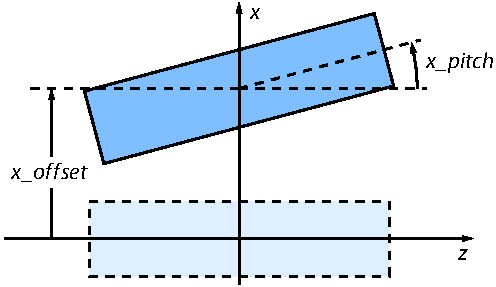
\includegraphics{pitch.eps}
  \caption{Geometry of Pitch and Offset attributes}
  \label{f:pitch}
\end{figure}

\begin{figure}[ht]
  \centering
  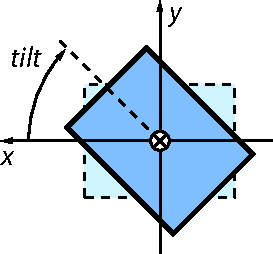
\includegraphics{tilt.eps}
  \caption{Geometry of a Tilt}
  \label{f:tilt}
\end{figure}

The tilt attribute rotates the element in the $(x, y)$ plane as shown
in figure~\ref{f:tilt}. The rotation axis is the $z$-axis at the
entrance face. The reference orbit is also rotated for any element
who's exit coordinates are not collinear with the entrance
coordinates. For example, a \vn{bend} or \vn{mirror} with a tilt of $\pi/2$ will bend a
beam vertically upward. The \vn{hkick} and \vn{vkick} attributes are
not affected by \vn{tilt} except for \vn{Kicker} and \vn{ElSeparator}
elements. Like MAD, \bmad allows the use of the \vn{tilt} attribute
without a value to designate a skew element. For example
\begin{example}
  q1: quad, l = 0.6, x_offset = 0.03, y_pitch = 0.001, tilt
\end{example}
Default tilts can be used for \vn{rbend}, \vn{sbend}, \vn{sol_quad},
\vn{quadrupole}, \vn{sextupole}, and \vn{octupole} elements.
The default tilt is $\pi/(2(n+1))$ where $n$ is the order of the 
element (n = 0 for bends, n = 1 for quadrupoles etc.) 

For all elements, offsets, pitches, and tilts are with
respect to the entrance coordinates (the local coordinates just before
the element.

The \vn{roll} attribute is only used for bends and rotates the bend,
along an axis that runs through the entrance point and exit point as
shown in figure~\ref{f:roll}. A \vn{roll} does not affect the
reference orbit. The major effect of a \vn{roll} is to give a vertical
kick to the beam. A positive \vn{roll} is similar to a positive
\vn{tilt}. That is, with a bend with positive bend angle, a positive
\vn{roll} will move the outside portion ($+x$ side) of the bend upward
and the inside portion (-$x$ side) downward. Much like car racetracks
which are typically slanted towards the inside of a turn.

\begin{figure}[ht]
  \centering
  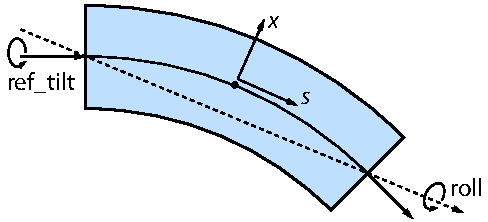
\includegraphics{roll.eps}
  \caption{Geometry of a Roll}
  \label{f:roll}
\end{figure}


%-----------------------------------------------------------------
\section{Hkick, Vkick, and Kick Attributes}
\label{s:kick}
\index{hkick|hyperbf}\index{bl_hkick|hyperbf}
\index{vkick|hyperbf}\index{bl_vkick|hyperbf}
\index{kick|hyperbf}\index{bl_kick|hyperbf}


\index{hkicker}
\index{vkicker}
\index{elseparator}
\index{kicker}
The kick attributes that an element may have are:
\begin{example}
  kick,  bl_kick  = <Real>  ! Used only with a Hkicker or Vkicker
  hkick, bl_hkick = <Real>
  vkick, bl_vkick = <Real>
\end{example}
\vn{kick}, \vn{hkick}, and \vn{vkick} attributes are the integrated
kick of an element in radians. \vn{kick} is only used for \vn{Hkicker}
and \vn{Vkicker} elements. All other elements that can kick use
\vn{hkick} and \vn{vkick}. The \vn{tilt} attribute will only rotate a
kick for \vn{Hkicker}, \vn{Vkicker}, \vn{Elseparator} and \vn{Kicker}
elements. This rule was implemented so that, for example, the
\vn{hkick} attribute for a skew quadrupole would represent a
horizontal steering. The \vn{bl_kick}, \vn{bl_hkick}, and
\vn{bl_vkick} attributes are the integrated field kick in
\vn{meters-Tesla}. Normally these are dependent attributes except if
they appear in the lattice file (\sref{s:depend}).

%-----------------------------------------------------------------
\section{Aperture and Limit Attributes}
\label{s:limit}
\index{aperture|hyperbf}
\index{limit|hyperbf}
\index{aperture_at|hyperbf}

\begin{figure}[ht]
  \centering
  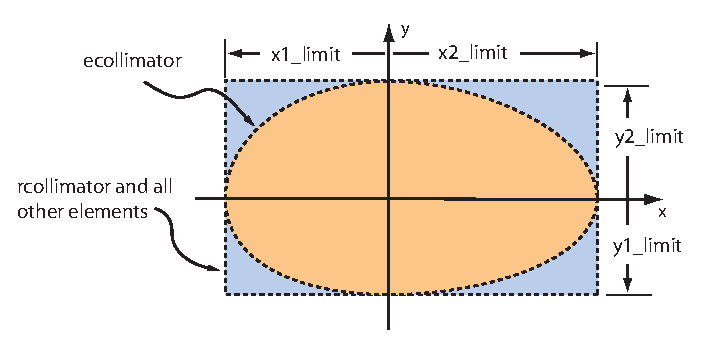
\includegraphics{apertures.eps}
  \caption{Apertures for ecollimator and rcollimator elements}
  \label{f:limit}
\end{figure}

\index{ecollimator}
\index{rcollimator}
\index{x_limit|hyperbf}
\index{y_limit|hyperbf}
\index{x1_limit|hyperbf}
\index{y1_limit|hyperbf}
\index{x2_limit|hyperbf}
\index{y2_limit|hyperbf}
\index{x_offset|hyperbf}
\index{offset_moves_aperture|hyperbf}
\index{aperture_at}
\index{aperture_type}
The aperture attributes are:
\begin{example}
  x1_limit      = <Real>      ! Horizontal, negative side, aperture limit
  x2_limit      = <Real>      ! Horizontal, positive side, aperture limit
  y1_limit      = <Real>      ! Vertical, negative side, aperture limit
  y2_limit      = <Real>      ! Vertical, positive side, aperture limit
  x_limit       = <Real>      ! Alternative to specifying x1_limit and x2_limit
  y_limit       = <Real>      ! Alternative to specifying y1_limit and y2_limit
  aperture      = <Real>      ! Alternative to specifying x_limit and y_limit
  aperture_at   = <Switch>    ! What end aperture is at.
  aperture_type = <Switch>    ! What type of aperture it is.
  offset_moves_aperture = <Logical> ! Element offsets affect aperture position
\end{example}
\vn{x1_limit}, \vn{x2_limit}, \vn{y1_limit}, and \vn{y2_limit} specify
the half--width of the aperture of an element as shown in
figure~\ref{f:limit}. A zero \vn{x1_limit}, \vn{x2_limit},
\vn{y1_limit}, or \vn{y2_limit} is interpreted as no aperture in the
appropriate plane.

By default, apertures are assumed to be
rectangular except that an \vn{Ecollimator} has a elliptical aperture.
This can be changed by setting the \vn{aperture_type} attribute. The possible 
values of this attribute are:
\begin{example}
  rectanular
  elliptical
\end{example}

To avoid numerical overflow and other errors in tracking, a particle
will be considered to have hit an aperture in an element, even if
there are no apertures set for that element, if its orbit exceeds 1000
meters. Additionally, there are other situations where a particle will
be considered lost. For example, if a particle's trajectory does
not intersect the output face in a bend.

For convenience, \vn{x_limit} can be used to set \vn{x1_limit} and
\vn{x2_limit} to a common value. Similarly, \vn{y_limit} can be used
to set \vn{y1_limit} and \vn{y2_limit}.  The \vn{aperture} attribute
can be use to set all four \vn{x1_limit}, \vn{x2_limit}, \vn{y1_limit}
and \vn{y2_limit} to a common value. Internally, the \bmad code does {\em not}
store \vn{x_limit}, \vn{y_limit}, or \vn{aperture}. This means that
using \vn{x_limit}, \vn{y_limit} or aperture in arithmetic expressions is
an error:
\begin{example}
  q2: quad, aperture = q1[aperture]   ! THIS IS AN ERROR!
  q2: quad, aperture = q1[x1_limit]   ! Correct
\end{example}

\index{tilt}
\index{x_offset}
\index{y_offset}
\index{x_pitch}
\index{y_pitch}
Normally, whether a particle hits an aperture or not is evaluated
independent of any element offsets (\sref{s:offset}). This is
equivalent to the situation where a beam pipe containing an aperture
is independent of the element the beam pipe passes through. This can
be changed by setting the \vn{offset_moves_aperture} attribute to
\vn{True}. In this case any offsets or pitches will be considered to
have shifted the aperture boundary. The exception here is that the
default for \vn{rcollimator} and \vn{ecollimator} elements is for
\vn{offset_moves_aperture} to be \vn{True}.

Even with \vn{offset_moves_aperture} set to \vn{True}, \vn{tilt}s will
not affect the aperture calculation. This is done, for example, so
that the tilt of a skew quadrupole does not affect the aperture. The
exception here is that tilting an \vn{rcollimator} or \vn{ecollimator}
element will tilt the aperture.

\index{entrance_end|hyperbf}
\index{exit_end|hyperbf}
\index{aperture_at}
By default the aperture is evaluated at the exit face only of the
element. This can be changed by setting the \vn{aperture_at} attribute.
Possible settings for \vn{aperture_at} are:
\begin{example}
  entrance_end
  exit_end  ! default
  both_ends
\end{example}
Note that the entrance and exit ends of an element are independent of
which direction particles are tracked through an element. Thus if a
particle is tracked backwards it enters an element at the ``exit end''
and exits at the ``entrance end''.

Examples:
\begin{example}
  q2: quad, aperture_type = elliptical  
  q1: quad, l = 0.6, x1_limit = 0.045, offset_moves_aperture = T
  q1[y1_limit] = 0.03
  q1[y2_limit] = 0.03
  q1[y_limit] = 0.03  ! equivalent to the proceeding 2 lines.  
  q1[aperture_at] = both_ends
\end{example}

%-----------------------------------------------------------------
\section{Length Attributes}
\label{s:l}

\index{l|hyperbf}
\index{l_chord|hyperbf}
\index{rbend}
\index{sbend}
The length attributes are
\begin{example}
  l       = <Real>  ! 
  l_chord           ! Chord length of a bend. Dependent attribute.
\end{example}
The length \vn{l} is the path length of the reference
particle. The one exception that that for an \vn{Rbend} the length
\vn{l} is the chord length (\sref{s:bend}). Internally, \bmad converts
all \vn{Rbend}s to \vn{Sbend}s and stores the chord length
under the \vn{l_chord} attribute.

\index{wiggler}
Note that for \vn{Wiggler}s
the length \vn{l} is not the same as the path length for a particle
with the reference energy starting on the reference orbit.

%-----------------------------------------------------------------
\section{Is_on Attribute}
\label{s:is.on}
\index{is_on|hyperbf}

The \vn{is_on} attribute
\begin{example}
  is_on = <Logical>
\end{example}
is used to turn an element off. Turning
an element off essentially converts it into a drift.
Example
\begin{example}
  q1: quad, l = 0.6, k1 = 0.95
  q1[is_on] = False
\end{example}

\vn{is_on} does not affect any apertures that are set. Additionally,
\vn{is_on} does not affect the reference orbit. Therefore, turning 
off an \vn{lcavity} will not affect the reference energy.

%-----------------------------------------------------------------
\section{Multipole Attributes: An, Bn, KnL, Tn}
\label{s:multip}

\index{multipole!an, bn|hyperbf} 
\index{multipole!knl, tn|hyperbf} 
\index{ab_multipole}
\index{multipole}
\index{radius}
A \vn{Multipole} element specifies its multipole components using an
Amplitude (\vn{KnL}) and a tilt (\vn{Tn})
\begin{example}
  KnL = <Real>
  Tn  = <Real>  ! Default is $pi$/(2n + 2)
\end{example}
\vn{AB_Multipole} and all other elements that
have multipole attributes specify the multipoles using normal
(\vn{Bn}) and skew (\vn{An}) components 
\begin{example}
  An = <Real>
  Bn = <Real>
\end{example}
Here \vn{n} ranges from 0
(dipole component) through 20. Example:
\begin{example}
  q1: quadrupole, b0 = 0.12, a20 = 1e7, radius = 0.045
\end{example}

Multipole formulas for are given in \sref{s:fields}.  Note that for
\vn{Multipole} and \vn{AB_multipole} (but not any other element) a
non-zero dipole component will affect the reference orbit (just like a
normal dipole will).

The \vn{Tn} tilt component without a value takes a default of $pi$/(2n + 2) which makes
the component \vn{skew}.
Example:
\begin{example}
  m: multipole, k1l = 0.45, t1  ! Skew quadrupole
\end{example}

For everything other than a \vn{Multipole} and \vn{AB_multipole}, the
multipole strength is scaled by a factor $F \, r_0^{n_\text{ref}} /
r_0^n$ (cf.~\Eq{ababf}) where $F$ is the strength of the element (for
example $F$ is $K1 \cdot L$ for a quadrupole), and $r_0$ is the
``measurement radius'' and is set by the \vn{radius} attribute. The
default value of $r_0$, if the \vn{radius} is not given, is 1.0.

%-----------------------------------------------------------------
\section{Instrumental Measurement Attributes}
\label{s:meas.attrib}

\index{instrument}\index{monitor}\index{marker}
\index{x_gain_err}\index{y_gain_err}\index{Crunch}\index{noise}
\index{x_gain_calib}\index{y_gain_calib}\index{crunch_calib}
\index{x_offset}\index{y_offset}\index{tilt}
\index{x_offset_calib}\index{y_offset_calib}\index{tilt_calib}
\index{de_eta_meas}\index{n_sample}\index{osc_amplitude}

\vn{Instrument}, \vn{Monitor}, and \vn{Marker} elements have special
attributes to describe orbit, betatron phase, dispersion and coupling
measurements. These attributes are:
\hfill\break
\hspace*{0.1in}
\begin{tabular}{llll}
  {\em Attribute}     &            &! {\em Symbol} (\sref{s:meas.calc}) & \\
  \vn{tilt}           &= <Real>    &! $\theta_t$            & See \sref{s:offset} \\ 
  \vn{x_offset}       &= <Real>    &! $x_{\mss{err}}$       & See \sref{s:offset} \\ 
  \vn{y_offset}       &= <Real>    &! $y_{\mss{err}}$       & See \sref{s:offset} \\ 
  \vn{x_gain_err}     &= <Real>    &! $dg_{x,\mss{err}}$    & Horizontal gain error \\ 
  \vn{y_gain_err}     &= <Real>    &! $dg_{y,\mss{err}}$    & Vertical gain error \\ 
  \vn{crunch}         &= <Real>    &! $\psi_{\mss{err}}$    & Crunch angle \\ 
  \vn{tilt_calib}     &= <Real>    &! $\theta_{\mss{err}}$  & tilt angle calibration \\ 
  \vn{x_offset_calib} &= <Real>    &! $x_{\mss{cal}}$       & Horizontal offset calibration \\ 
  \vn{y_offset_calib} &= <Real>    &! $y_{\mss{cal}}$       & Vertical offset calibration \\ 
  \vn{x_gain_calib}   &= <Real>    &! $dg_{x,\mss{cal}}$    & Horizontal gain calibration \\ 
  \vn{y_gain_calib}   &= <Real>    &! $dg_{y,\mss{cal}}$    & Vertical gain calibration \\ 
  \vn{crunch_calib}   &= <Real>    &! $\psi_{\mss{cal}}$    & Crunch angle calibration \\ 
  \vn{noise}          &= <Real>    &! $n_f$                 & Noise factor \\ 
  \vn{de_eta_meas}    &= <Real>    &! $dE/E$                & Percent change in energy \\ 
  \vn{n_sample}       &= <Real>    &! $N_s$                 & Number of sampling points \\ 
  \vn{osc_amplitude}  &= <Real>    &! $A_{\mss{osc}}$       & Oscillation amplitude \\ 
\end{tabular}
\hfill\break
A program can use these quantities to calculate ``measured'' values from the
``laboratory'' values. Here, ``laboratory'' means as calculated from some model lattice.
See \sref{s:meas.calc} for the conversion formulas.

\chapter{Tracking and Transfer Matrix Calculation Methods}

Typically, there are several ways to do tracking and transfer matrix
calculations for a given element type within \bmad. What method is
used is selected on an element--by--element basis using an element's
\vn{tracking_method} and \vn{mat6_calc_method} attributes (mat6 refers
to the size of the 6 by 6 transfer matrices). By supplying the
appropriate routines a programmer can extend \bmad\ to do customized
tracking. In general \bmad assumes that particles are
ultra--relativistic. The methods that do not make this assumption are:
\vn{Boris}, \vn{Adaptive_Boris}, \vn{Symp_Lie_Ptc}, \vn{Symp_map}, and \vn{Taylor}

If this is not the case 

%----------------------------------------------------------------------------
\section{tracking\_method Switches}
\label{s:tkm}
\index{Tracking method|textbf}

Below are listed the methods for the \vn{tracking_method}
attribute with an explanation of what the different methods do. A
table giving which methods are available with which element types is give
in Table~\ref{t:track_methods}. 

A note on terminology: Adaptive step size control used with the
\vn{Adaptive_Boris} and \vn{Runge_Kutta} integrators means that 
instead of taking fixed step sizes the integrator chooses the proper
step size so that the error in the tracking is below the maximum
allowable error set by \vn{rel_tol} and \vn{abs_tol} tolerances. The
advantage of step size control is that the integrator uses a smaller
step size when needed (the fields are rapidly varying), but makes
larger steps when it can. The disadvantage is that a step is more
computationally intensive since the error in a step is estimated by
repeating a step using two mini steps. If the fields are rather
uniform and you know what a good step size is you can save time by using
a fixed step size.

\begin{description}
\item[\vn{Adaptive\_Boris}]
Second order Boris integration\cite{b:boris} with adaptive step size control.
This should be nearly symplectic but slow.

\item[\vn{Boris}]
Second order Boris Integration\cite{b:boris}. Like \vn{Runge_Kutta},
\vn{Boris} does tracking by integrating the equation of
motion. \vn{Boris} handles both electric and magnetic fields and does
not assume that the particle is ultra--relativistic. \vn{Boris} preserves
conserved quantities more accurately than \vn{Runge_Kutta}.

\item[\vn{Bmad\_Standard}]
Uses formulas for tracking. The emphasis here is on speed and not
symplecticity. Appropriate when you are interested in single turn
stuff. May be appropriate for long term tracking depending upon how
many turns are tracked and what kind of elements are involved. 

\item[\vn{Custom}]
This method will call a routine \vn{track1_custom} which must be
supplied by the programmer implementing the custom tracking. The
default \vn{track1_custom} supplied with the \bmad\ release will print
an error message and stop the program if it is called which probably
indicates a program linking problem.

\item[\vn{Linear}]
Linear just uses the 0th order vector with the 1st order 6x6 transfer
matrix for an element. Very simple.  Depending upon how the transfer
matrix was generated this may or may not be symplectic.

\item[\vn{MAD}]
This uses the MAD 2nd order transfer map.

\item[\vn{Runge\_Kutta}]
This uses a 4\Th\ order Runge Kutta integration algorithm with adaptive
step size control.  This is essentially the \vn{ODEINT} subroutine
from Numerical Recipes\cite{b:nr}. This may be slow but it should be
accurate. This method is non-symplectic.

\item[\vn{Symp\_Lie\_Bmad}]
Symplectic tracking using a Hamiltonian with Lie operation techniques.
This is similar to \vn{Symp_Lie_PTC} (see below) except this uses a
\bmad\ routine. By bypassing some of the generality inherent in PTC's routines
\vn{Symp_Lie_Bmad} achieves about a factor of 10 improvement in speed over
\vn{Symp_Lie_PTC}. However, \vn{Symp_lie_Bmad} is
currently only implemented for Wigglers.

\item[\vn{Symp\_Lie\_PTC}]
Symplectic tracking using a Hamiltonian with Lie operator techniques.
This uses Etienne's PTC software for the calculation. This method is
symplectic but can be slow.

\item[\vn{Symp\_Map}]
This uses a partially inverted, implicit Taylor map. The calculation
uses Etienne's PTC software.  Since the map is implicit, a Newton
search method must be used. This will slow things down from the Taylor
method but this is guaranteed symplectic.

\item[\vn{Taylor}]
This uses a Taylor map generated from Etienne's PTC
package. Generating the map may take time but once you have it it
should be very fast. One possible problem with using a Taylor map is
that you have to worry about the accuracy if you do tracking at points
that are far from the expansion point about which the map was
made. This method is non-symplectic away from the expansion point. 

\item[\vn{Wiedemann}]
This is Wiedemann's hard edge model of a wiggler
\cite{wiedemann}. This model divides a wiggler pole into a constant 
bend rectangular section with drifts at either end. The total length
of the model pole matches the actual pole length of the element. The
strength of the bend and the lengths of the bend and drifts are
adjusted so that the vertical focusing and horizontal deflection are
the same in the modal as with a model assuming a sinusoidally varying
field. \bmad\ augments this model by assuming that the horizontal
deflection varies as the $\sinh$ with vertical offset.  Since
Wiedemann's model does not include longitudinal fields it is not clear
that it can be used for long term tracking.

\end{description}

\vfill \break
{\vfill}

\begin{table}[h]
\centering {
\begin{tabular}{|l|c|c|c|c|c|c|c|c|c|c|c|c|} \hline
\rule{0pt}{80pt} &
\begin{sideways}\vn{Adaptive_Boris}\end{sideways} &
\begin{sideways}\vn{Bmad_Standard}\end{sideways} &
\begin{sideways}\vn{Boris}\end{sideways} &
\begin{sideways}\vn{Custom}\end{sideways} &
\begin{sideways}\vn{Linear}\end{sideways} &
\begin{sideways}\vn{MAD}\end{sideways} &
\begin{sideways}\vn{Runge_Kutta}\end{sideways} &
\begin{sideways}\vn{Symp_Lie_Bmad}\end{sideways} &
\begin{sideways}\vn{Symp_Lie_PTC}\end{sideways} &
\begin{sideways}\vn{Symp_Map}\end{sideways} &
\begin{sideways}\vn{Taylor}\end{sideways} &
\begin{sideways}\vn{Wiedemann}\end{sideways}
\\ \hline
%                               AB  BS   B   C   L   M  RK  SLB SLP SM   T   W
  \vn{ab_multipole}            &   & D &   & X & X &   &   &   & X & X & X &   \\ \hline 
  \vn{beambeam}                &   & D &   & X & X &   &   &   &   &   &   &   \\ \hline 
  \vn{bend_sol_quad}           &   &   &   &   &   &   &   & D &   &   &   &   \\ \hline 
  \vn{custom}                  & X &   & X & D & X &   & X &   &   &   &   &   \\ \hline 
  \vn{drift}                   & X & D & X & X & X & X & X &   & X & X & X &   \\ \hline 
  \vn{ecollimator}             & X & D & X & X & X &   & X &   & X & X & X &   \\ \hline 
  \vn{elseparator}             & X & D & X & X & X & X & X &   & X & X & X &   \\ \hline 
  \vn{hkicker}                 & X & D & X & X & X &   & X &   & X & X & X &   \\ \hline 
  \vn{instrument}              & X & D & X & X & X &   & X &   & X & X & X &   \\ \hline 
  \vn{kicker}                  & X & D & X & X & X &   & X &   & X & X & X &   \\ \hline 
  \vn{lcavity}                 &   & D &   & X & X &   &   &   &   &   &   &   \\ \hline 
  \vn{marker}                  &   & D &   & X & X &   &   &   & X & X & X &   \\ \hline 
  \vn{monitor}                 & X & D & X & X & X &   & X &   & X & X & X &   \\ \hline 
  \vn{multipole}               &   & D &   & X & X &   &   &   & X & X & X &   \\ \hline 
  \vn{octupole}                & X & D & X & X & X &   & X &   & X & X & X &   \\ \hline
  \vn{patch}                   &   & D &   & X &   &   &   &   &   &   &   &   \\ \hline
  \vn{quadrupole}              & X & D & X & X & X & X & X &   & X & X & X &   \\ \hline
  \vn{rbend}                   &   & D &   & X & X & X &   &   & X & X & X &   \\ \hline
  \vn{rcollimator}             & X & D & X & X & X &   & X &   & X & X & X &   \\ \hline
  \vn{rfcavity}                &   & D &   & X & X & X &   &   & X & X & X &   \\ \hline
  \vn{sbend}                   &   & D &   & X & X & X &   &   & X & X & X &   \\ \hline
  \vn{sextupole}               & X & D & X & X & X & X & X &   & X & X & X &   \\ \hline
  \vn{solenoid}                & X & D & X & X & X & X & X &   & X & X & X &   \\ \hline
  \vn{sol_quad}                & X & D & X & X & X & X & X &   & X & X & X &   \\ \hline
  \vn{taylor}                  &   & D &   & X & X &   &   &   &   &   &   &   \\ \hline
  \vn{vkicker}                 & X & D & X & X & X &   & X &   & X & X & X &   \\ \hline
  \vn{wiggler} (periodic type) &   & D &   & X & X &   &   &   &   &   &   & X \\ \hline
  \vn{wiggler} (map type)      & X & D & X & X & X &   & X & X & X & X & X &   \\ \hline
\end{tabular}
}
\caption[Table of available {\bf tracking\_method}\ switches for a
given element type.]{Table of available {\bf tracking\_method}\
switches for a given element type. D denotes the default method. X
denotes an available method.}
\label{t:track_methods}
\end{table}

\vfill\break

%----------------------------------------------------------------------------
\section{mat6\_calc\_method Switches}
\label{s:xfer}
\index{Mat6_calc_method|textbf}

Below are listed the methods for the \vn{mat6_calc_method}
attribute with an explanation of what the different methods do. A
table giving which methods are available with which element types is give
in Table~\ref{t:mat6_methods}. 

For methods that do not necessarily produce a symplectic matrix the
\vn{symplectify} attribute of an element can be set to \vn{True} to
solve the problem. See section~\ref{s:symp_method}. 

Symplectic integration is like ordinary integration of a function f(x)
but what is integrated here is a Taylor map. Truncating the map to
0\Th\ order gives the particle trajectory and truncating to 1\St\
order gives the transfer matrix (Jacobian).  The order at which a
Taylor series is truncated at is set by \vn{taylor_order} (see
Section~\ref{s:param}. Like ordinary integration there are various
formulas that one can use to do symplectic integration. In \bmad\ (or
more precisely Etienne's PTC) you can use one of 3 methods. This is
set by \vn{integration_ord}.  \vn{integration_ord} = n where $n$ is
allowed by PTC to be 2, 4, or 6. With an integration order of $n$ the
error in an integration step scales as $dz^n$ where $dz$ is step
size. The step size $dz$ is set by the length of the element and the
value of \vn{num_steps}. Remember, as in ordinary integration, higher
integration order does not necessarily imply higher accuracy.

\begin{description}

\index{Mat6_calc_method!Bmad_Standard}
\item[\vn{Bmad\_Standard}]
Uses formulas for the calculation. The emphasis here is on speed and not
symplecticity. Appropriate when you are interested in single turn
stuff. May be appropriate for long term tracking depending upon how
many turns are tracked and what kind of elements are involved. 

\index{Mat6_calc_method!Custom}
\item[\vn{Custom}]
This method will call a routine \vn{make_mat6_custom} which must be
supplied by the programmer implementing the custom transfer matrix
calculation. The default \vn{make_mat6_custom} supplied with the
\bmad\ release will print an error message and stop the program if it
is called which probably indicates a program linking problem.

\index{Mat6_calc_method!MAD}
\item[\vn{MAD}]
This uses the MAD 2nd transfer map.

\index{Mat6_calc_method!Symp_lie_Bmad}
\item[\vn{Symp\_Lie\_Bmad}]
A Symplectic calculation using a Hamiltonian with Lie operator techniques.
This is similar to \vn{Symp_Lie_PTC} (see below) except this uses a
\bmad\ routine. By bypassing some of the generality inherent in PTC's routines
\vn{Symp_Lie_Bmad} achieves about a factor of 10 improvement in speed over
\vn{Symp_Lie_PTC}. However, \vn{Symp_lie_Bmad} is
currently only implemented for Wigglers.

\index{Mat6_calc_method!Symp_Lie_PTC}
\item[\vn{Symp\_Lie\_PTC}]
Symplectic integration using a Hamiltonian and Lie operators.
This uses Etienne's PTC software for the calculation.
This method is symplectic but can be slow.

\index{Mat6_calc_method!Taylor}
\item[\vn{Taylor}]
This uses a Taylor map generated from Etienne's PTC
package. Generating the map may take time but once you have it it
should be very fast. One possible problem with using a Taylor map is
that you have to worry about the accuracy if you do a calculation at points
that are far from the expansion point about which the map was
made. This method is non-symplectic away from the expansion point. 

\index{Mat6_calc_method!Tracking}
\item[\vn{Tracking}]
This uses the tracking method set by \vn{tracking_method} to track 6
particles around the central orbit. This method is susceptible to inaccuracies
caused by nonlinearities. Furthermore this method
is almost surely slow. While non--symplectic, the advantage of this method
is that it is directly related to any tracking results.

\end{description}

\vfill \break
\vfill

\begin{table}[th]
\centering {
\begin{tabular}{|l|c|c|c|c|c|c|c|} \hline
\rule{0pt}{80pt} &
\begin{sideways}\vn{Bmad_Standard}\end{sideways} &
\begin{sideways}\vn{Custom}\end{sideways} &
\begin{sideways}\vn{MAD}\end{sideways} &
\begin{sideways}\vn{Symp_Lie_Bmad}\end{sideways} &
\begin{sideways}\vn{Symp_Lie_PTC}\end{sideways} &
\begin{sideways}\vn{Taylor}\end{sideways} &
\begin{sideways}\vn{Tracking}\end{sideways}
\\ \hline
%                               BS   C   M  SLB SLP Tlr Trk 
  \vn{ab_multipole}            & D & X &   &   & X & X &   \\ \hline 
  \vn{beambeam}                & D & X &   &   &   &   & X \\ \hline 
  \vn{bend_sol_quad}           &   &   &   & D &   &   & X \\ \hline 
  \vn{custom}                  &   & D &   &   &   &   & X \\ \hline 
  \vn{drift}                   & D & X & X &   & X & X & X \\ \hline 
  \vn{ecollimator}             & D & X &   &   & X & X & X \\ \hline 
  \vn{elseparator}             & D & X & X &   & X & X & X \\ \hline 
  \vn{hkicker}                 & D & X &   &   & X & X & X \\ \hline 
  \vn{instrument}              & D & X &   &   & X & X & X \\ \hline 
  \vn{kicker}                  & D & X &   &   & X & X & X \\ \hline 
  \vn{lcavity}                 & D & X &   &   &   &   & X \\ \hline 
  \vn{marker}                  & D & X &   &   & X & X & X \\ \hline 
  \vn{monitor}                 & D & X &   &   & X & X & X \\ \hline 
  \vn{multipole}               & D & X &   &   & X & X &   \\ \hline 
  \vn{octupole}                & D & X &   &   & X & X & X \\ \hline
  \vn{patch}                   & D & X &   &   &   &   &   \\ \hline
  \vn{quadrupole}              & D & X & X &   & X & X & X \\ \hline
  \vn{rbend}                   & D & X & X &   & X & X & X \\ \hline
  \vn{rcollimator}             & D & X &   &   & X & X & X \\ \hline
  \vn{rfcavity}                & D & X & X &   & X & X & X \\ \hline
  \vn{sbend}                   & D & X & X &   & X & X & X \\ \hline
  \vn{sextupole}               & D & X & X &   & X & X & X \\ \hline
  \vn{solenoid}                & D & X & X &   & X & X & X \\ \hline
  \vn{sol_quad}                & D & X & X &   & X & X & X \\ \hline
  \vn{taylor}                  & D & X &   &   &   &   &   \\ \hline
  \vn{vkicker}                 & D & X &   &   & X & X & X \\ \hline
  \vn{wiggler} (periodic type) & D & X &   &   &   &   & X \\ \hline
  \vn{wiggler} (map type)      & D & X &   & X & X & X & X \\ \hline
\end{tabular}
}

\caption[Table of available \vn{mat6\_calc\_method}\ switches for a
given element type.]{Table of available \vn{mat6\_calc\_method}\
switches for a given element type. D denotes the default method.  X
denotes an available method.}

\label{t:mat6_methods}
\end{table}

\vfill \break

\chapter{Beam Lines and Lists}

An input lattice to \bmad\ is a sequence of physical elements which
will be called a beam line. Beam lines are defined by using two
constructs called lines and lists. This is very similar to \mad lines
and lists. There can be mulitiple beam lines and lists defined in a
lattice file and lines and lists can be nested inside other beam
lines. The particular beam line that defines the lattice to be used by
\bmad\ is selected by the \vn{use} statement. For example
\begin{example}
  use, my_line
\end{example}
would pick the line \vn{my_line}.

\section{Beam Lines}
A beam line without arguments (beam lines with arguments will be
discussed below) has the format
\begin{example}
  label: LINE = (member1, member2, ...)
\end{example}
where \vn{member1}, etc. are either elements, or other beam lines or lists.
Example:
\begin{example}
  this: line = (a, b, c, a)
  use, this
\end{example}
The \vn{use} command defines the lattice to be the sequence \vn{a, b, c, a}.

Lines can be nested within lines:
\begin{example}
  a: line = (a1, a2)
  b: line = (b1, a)
  c: line = (b, c1, a)
  use, c
\end{example}
This results in the lattice being
\begin{example}
  c = (b1, a1, a2, c1, a1, a2)
\end{example}

For lines

\chapter{Miscellaneous Commands}

This chapter deals with the commands not covered in the previous chapters.

%-----------------------------------------------------------------------------------
\section{Parameter Command}

The \vn{parameter} command is used to set the \vn{lattice} name and other variables. 
The variables that can be set by \vn{parameter} is
\begin{example}
  parameter[lattice]      = String 
  parameter[lattice_type] = Switch      ! default: circular_lattice
  parameter[taylor_order] = Integer     ! default: 3
  parameter[beam_energy]  = Real        ! default: 0
  parameter[symmetry]     = Switch      ! default: no_symmetry 
\end{example}

\noindent
Examples
\begin{example}
  parameter[lattice]      = "L9A19C501.FD93S_4S_15KG"
  parameter[lattice_type] = circular_lattice
  parameter[taylor_order] = 5
  parameter[beam_energy]  = 5.6e9    ! eV
  parameter[symmetry]     = no_symmetry
\end{example}

%-----------------------------------------------------------------------------------
\section{Beam Command}
\label{s:beam}

The \vn{lattice} name is stored by \bmad\ for use by a program but it does
not otherwise effect any \bmad\ routines. 
Historically it is possible to set the lattice name using the syntax
\begin{example}
  lattice = String   ! DO NOT USE THIS SYNTAX
\end{example}
This syntax is obsolete since a typographical error is not easily caught.

\noindent
Valid \vn{lattice_type} switches are
\begin{example}
  circular_lattice  ! default
  linear_lattice
  linac_lattice
\end{example}
a \vn{circular_lattice} is for a closed ring where one expects a periodic
solution for the Twiss parameters. A \vn{linear_lattice} is not closed
so that the initial Twiss parameters need to be given, not computed. A
\vn{linac_lattice} is a linear lattice with \vn{lcavity} elements.

The Taylor order (cf.~\ref{s:taylor_phys}) is the maximum order for a Taylor map.
Historically it is possible to set the taylor order using the syntax
\begin{example}
  taylor_order = Integer   ! DO NOT USE THIS SYNTAX
\end{example}
This syntax is obsolete since a typographical error is not easily caught.

The \vn{beam_energy} is the reference energy.  Each element in a lattice 
has an individual reference energy. For a circular or linear lattice all 
the reference energies are the same. For a linac lattice
the reference energy changes between \vn{lcavities}.

The \vn{symmetry} variable is used to set the symmetry of the lattice.
Historically it was used with the Cornell CESR ring but it has fallen 
out of favor (mainly since CESR has no symmetry nowadays) and its use
is currently discouraged. Valid \vn{symmetry} switches are
\begin{example}
  no\_symmetry         ! default
  mobius\_symmetry
  ew\_antisymmetry
  ew\_symmetry
\end{example}


%-----------------------------------------------------------------------------------
\section{Beam Command}

The \vn{Beam} command is provided for compatibility with \mad. The syntax is
\begin{example}
  beam, energy = GeV, particle = Switch, n_part = Real
\end{example}
For example
\begin{example}
  beam, energy = 5.6  ! Note: Gev to be compatible with \mad
  beam, particle = electron, n_part = 1.6e10
\end{example}
Setting the reference energy using the \vn{energy} attribute is the same
as using \vn{parameter [beam_energy]}. Valid \vn{particle}
switches are
\begin{example}
  positron  ! default
  electron
\end{example}

%-----------------------------------------------------------------------------------
\section{Title Command}
The \vn{title} command sets a title string which can be used by a program. 
For consistency there are two possible syntaxes
\begin{example}
  title, String
\end{example}
or
\begin{example}
  title
  String
\end{example}
For example
\begin{example}
  title
  "This is a title"
\end{example}

%-----------------------------------------------------------------------------------
\section{Call Command}

It is typically convenient to separate the lattice definition into several files.
Typically there might be a file (or files) that define the layout of the lattice
(something that doesn't change often) and a file (or files) that define magnet strengths
(something that changes more often).
The \vn{call} is used to read in separated lattice files. The syntax is
\begin{example}
  call, filename = String
\end{example}
Example
\begin{example}
  call, filename = "../layout/my_layout.bmad"
\end{example}
\bmad\ will read the called file until a \vn{return} or \vn{end_file} command is encountered
or the end of the file is reached.

%-----------------------------------------------------------------------------------
\section{Return and End\_File Commands}

\vn{Return} and \vn{end_file} have identical effect and tell \bmad\ to ignore anything
beyond the \vn{return} or \vn{end_file} command in the file.

%-----------------------------------------------------------------------------------
\section{Beginning Command}

For non--circular lattices the \vn{beginning} command can be used to set the Twiss parameters 
and beam energy at the beginning of the ring 
\begin{example}
  beginning[beta_x]  = Real  ! "a" mode beta
  beginning[alpha_x] = Real  ! "a" mode alpha
  beginning[phi_x]   = Real  ! "a" mode phase
  beginning[eta_x]   = Real  ! "a" mode dispersion
  beginning[etap_x]  = Real  ! "a" mode dispersion derivative.
  beginning[beta_y]  = Real  ! "b" mode beta
  beginning[alpha_y] = Real  ! "b" mode alpha
  beginning[phi_y]   = Real  ! "b" mode phase
  beginning[eta_y]   = Real  ! "b" mode dispersion
  beginning[etap_y]  = Real  ! "b" mode dispersion derivative.
  beginning[cij]     = Real  ! C coupling matrix. i, j = {``1'', or ``2''} 
  beginning[energy]  = Real  ! Total energy in eV.
\end{example}
The \vn{gamma_x}, \vn{gamma_y}, and \vn{gamma_c} (the coupling gamma factor) 
will be kept consistent with the values set. If not set the default values are all zero. 

For any lattice the \vn{beginning} command can be used to set the starting floor position 
(see~\ref{s:global}). The syntax is
\begin{example}
  beginning[x_position]     = Real  ! X position
  beginning[y_position]     = Real  ! Y position
  beginning[z_position]     = Real  ! Z position
  beginning[theta_position] = Real  ! Angle on floor
  beginning[phi_position]   = Real  ! Angle of attack
\end{example}

%-----------------------------------------------------------------------------------
\section{Parser\_Debug Command}

The \vn{parser_debug} command is used to diagnose problems with the \bmad\ parser 
routine. That is, it is generally only used by programmers. 
It is recommended that this
command be used with small test lattices since it can generate a lot of output.
The syntax is
\begin{example}
  parser\_debug Switches
\end{example}
Valid switches are
\begin{example}
  var     ! print variable information
  seq     ! print sequence information
  slave   ! print full information on all regular elements
  lord    ! print full information on all lord elements
  ring    ! print a list of regular element names, positions, and lengths
\end{example}
Example
\begin{example}
  parser\_debug var ring
\end{example}


%-----------------------------------------------------------------------------------
\section{No\_Digested Command}

The \vn{no_digested} command if present, will prevent \bmad\ from 
creating a digested file. This can be helpful for debugging purposes but
otherwise it is not generally used.




%----------------------------------------------------------------
\part{Programmer's Guide}
%----------------------------------------------------------------
\chapter{Introduction to BMAD programming}

\section{The BMAD Distribution}

The \bmad\ software uses other software packages. \bmad, along with the packages it uses, 
is bundled together to form what is called the \bmad\ distribution. The \bmad\ distribution
also includes example lattice files and example programs. The \bmad\ distribution includes a custimized version of the Fortran90 version of Numerical Recipes\cite{nr}. It is the obligation of anyone who uses \bmad\ to make sure that they have the appropriate licance for Numerical Recipes. 

Also included in the distribution is the PGPLOT plotting package developed by Tim Pearson of CalTech.
PGPLOT is freely available for non-commercial use. PGPLOT is not public--domain software and is copyrighted by the California Institute of Technology further documentation can be found at
\begin{example}
    http://www.astro.caltech.edu/~tjp/pgplot
\end{example}
The advantage of PGPLOT is that it provides a set of device--independent routines making it very flexible and portable. To simplify the interface a set of wrapper subroutines call Quick_Plot are
included in the \bmad\ distribution. This is discussed later.

The other package used by \bmad\ is FPP/PTC written by Etienne Forest. This software can do 
various differential and lie algebraic operations as well as truncated power series algebra. further
documentation can be found at
\begin{example}
    http://bc1.lbl.gov/CBP_pages/educational/TPSA_DA/Introduction.html
\end{example}

%-----------------------------------------------------------------------------
\section{Getf and Listf}

As can be seen there is a lot going on behind the scenes even for this
simple program.This shows that programming with \bmad\ can be both easy
and hard. Easy in the sense that a lot can be done with just a few
lines. The hard part comes about since there are many details that
have to be keept in mind in order to make sure that the subroutines
are calculating what you want them to calculate.

To help with the details all \bmad\ subroutines have in their source (.f90)
files a comment block that explains the arguments needed by the
subroutines and explains what the subroutine does. To help quickly
access these comments there are two perl scripts that are supplied
with the \bmad\ distribution that are invloked with the commands
\cmd{listf} and \cmd{getf}.

The \cmd{listf} command is used to locate routines and structures.
The form of the command is
\begin{verbatim}
    listf <name>
\end{verbatim}
This searches for any routine or structure with the name
<name>. <name> may contain the wild--cards ``*'' and ``\%'' where
``*'' matches to any number of characters and ``\%'' matches to any
single character. For example:
\begin{verbatim}
    listf ring_struct
    listf twiss_at_%
\end{verbatim}
The second example will match to \rn{twiss_at_s} but not
\rn{twiss_at_start}.

The \cmd{getf} command is like the \cmd{listf} command with the
addition that the header comments that are in the source code files
will be printed out for each routine match and the structure definition
will be printed for each structure matched. The \cmd{getf} command is
thus more verbose than the \cmd{listf} command.

%-----------------------------------------------------------------------------
\section{Porgramming Conventions}

\bmad\ subroutines follow the following conventions:

\begin{description}
\item[\$ Denotes Parameter] A ``\$'' at the end of a name denotes an 
integer parameter. For example, in the above example program, to check
whether an element is a quadrupole one would write:
\begin{verbatim}
  if (ring%ele_(i)%key == quadrupole$) ...
\end{verbatim}
Checking the source code one would find in the module \tn{bmad_struct}
\begin{verbatim}
  integer, parameter :: drift$ = 1, sbend$ = 2, quadrupole$ = 3, group$ = 4
\end{verbatim}
One should always use the parameter name instead of the integer it represents.
That is, one should never write
\begin{verbatim}
  if (ring%ele_(i)%key == 3) ...  ! DO NOT DO THIS!
\end{verbatim}
For one, using the name makes the code clearer but more importantly
the exact value of the parmeters may at times be shuffled which would
lead to disasterous results if the values themselves were coded into a
program.

\item[ Type names have a \_struct suffix]. For example: \tn{ring_struct}, 
\tn{ele_struct}, etc.

\end{description}

%-----------------------------------------------------------------------------
\section{A First Program}

Let us start with a simple test program:
\begin{verbatim}
program test
  use bmad                 ! Define the structures we need to know about.
  implicit none
  type (ring_struct) ring  ! This structure holds the lattice info
  integer i
  character(200) lat_file
!
  lat_file = "/home/cesrulib/cesr_libs/current/" // &
                "config/bmad/lat/bmad_L9A18A000-_MOVEREC.lat"
  call bmad_parser (lat_file, ring)    ! Read in a lattice.
  call twiss_at_start (ring)           ! Calculate starting Twiss params.
  call twiss_propagate_all (ring)      ! Propagate Twiss parameters
  print *, ' Ix  Name              Ele_type                   S      Beta_x'
  do i = 0, ring%n_ele_ring
    print '(i4, 2x, a, 2x, a, 2f12.4)', i, ring%ele_(i)%name, &
                    key_name(ring%ele_(i)%key)&
                    ring%ele_(i)%s, ring%ele_(i)%x%beta
  enddo
end program
\end{verbatim}

The \cs{use bmad} statement defines the \bmad\ structures (types)
and defines the interfaces (argument lists) for the \bmad\
subroutines. In particular, the \tn{ring_struct} structure holds all the
lattice information: The list of elements, their attributes,
etc. \rn{bmad_parser} is the routine to parse a particular lattice file and
transfer the information to a \tn{ring_struct}\. After it is called the
program uses \rn{twiss_at_start} to multiply the transfer matrices
of the individual elements together to form the 1--turn matrix from
the start back to the start. From this \rn{twiss_at_start}
calculates the Twiss parameters at the start of the lattice. The next
call to \rn{twiss_propagate_all} takes the starting Twiss parameters
and using the transfer matrices of the individual elements calculates
the Twiss parameters at all the elements. We are now ready for the
print out the calculation. \vn{ring} has within it an array
\vn{ring%ele_(0:)} that contains the infomation on each individual
element. \vn{ring%ele_(0)} is basically a marker element to denote
the beginning of the array. \vn{ring%ele_(i)%key} is an integer
denoting what type of element (quadrupole, wiggler, etc.) it is.
\vn{ring%ele_(i)%s} is the longitudinal position at the end of an 
element. \vn{ring%ele_(i)%x%beta} is the $a$--mode (nearly
horizontal mode) beta.


\chapter{Reading and Writing Lattices}

%----------------------------------------------------------------------------
\section{Reading in Lattices}
\index{Lattice files!reading}

The subroutine to read in an XSIF lattice file is \vn{xsif_parser}.
There are two subroutines in \bmad\ to read in a \bmad standard
lattice file: \vn{bmad_parser} and \vn{bmad_parser2}.

\vn{bmad_parser} is used to initialize a \vn{ring_struct}
structure from scratch using the information from a lattice
file. Unless told otherwise, after reading in the lattice
\vn{bmad_parser} will compute the 6x6 transfer matrices for each
element. Normally you want to do this but there are exceptions where
you don't need it and for particular lattices the computation can take
a long time (especially if there are Taylor maps to be
computed). Notice that \vn{bmad_parser} does {\em not} compute any
Twiss parameters.

\vn{bmad_parser2} is typically used after \vn{bmad_parser} if there is
additional information that needs to be added to the lattice. For
example, aperture limits for the elements are often stored in a
separate file. In this case there are two possibilities: The first is
to use \vn{bmad_parser2}
\begin{verbatim}
  call bmad_parser ('lattice_file', ring)       ! read in a lattice.
  call bmad_parser2 ('aperture_file', ring)     ! read in the aperture limits.
\end{verbatim}
The second alternative is to create a third file that calls the first two
\begin{verbatim}
 ! This is a file to be called by bmad_parser
 call, file = 'lattice_file'
 call, file = 'aperture_file'
\end{verbatim}
and then just use \vn{bmad_parser} to parse this third file.

%----------------------------------------------------------------------------
\section{Digested Files}
\index{Lattice files!digested files}

Since parsing can be slow, once \vn{bmad_parser} has transfered the
information from a lattice file into the \vn{ring_struct} it will make
what is called a digested file. A digested file is an image of the
\vn{ring_struct} in binary form. When \vn{bmad_parser} is called it
(actually it is a the subroutine \vn{read_digested_bmad_file} that
does all the work) first looks in the same directory as the lattice
file for a digested file whose name is of the form
\begin{verbatim}
  'digested_' // LAT_FILE   ! for single precision BMAD 
  'digested8_' // LAT_FILE  ! for double precision BMAD 
\end{verbatim}
where \vn{LAT_FILE} is the lattice file name. If it finds the digested
file it checks that the file is not out--of--date. It can do this
since the digested file stores the names and the dates of all the
lattice files that were used when the digested file was made. The
\bmad\ version number stored in the digested file is also checked. The
\bmad\ version number is a global parameter that is increased (not too
frequently) each time the structure of the \vn{ring_struct} or
\vn{ele_struct} is modified. If the \bmad\ version number in the
digested file does not agree with the current or the digested file is
out--of--date a warning will be printed and the digested file will not
be used.

\index{Transfer map!Taylor!with digested files}
Since computing Taylor Maps can be very time intensive,
\vn{bmad_parser} tries to reuse Taylor Maps it finds in the digested
file even if the lattice file has been changed in the meantime. To
make sure that everything is OK it will check that the attribute
values of an element needing a Taylor map are the same as the
attribute values of a corresponding element in the digested file
before it reuses the map. Element names are not a factor in this
decision.

This leads to the following trick: If you want to read in a lattice
where there is no corresponding digested file, and if there is another
digested file that has elements with the correct Taylor Maps, then to
save on the map computation time simply make a copy of the digested
file with the digested file name corresponding to the first lattice.

The digested file is in binary format and is not human readable but it
provides a convenient mechanism for transporting lattices between
programs. For example, say you have read in a lattice, changed
some parameters in the \vn{ring_struct}, and now you want to do some
analysis on this modified \vn{ring_struct} using a different program. The 
answer is to have the first program create a digested file
\begin{example}
  call write_digested_bmad_file ('digested_file_of_mine', ring)
\end{example}
and then read the digested file in with the second program
\begin{example}
  call read_digested_bmad_file ('digested_file_of_mine', ring)
\end{example}
An alternative to writing a digested file is to write a lattice file
using \vn{write_bmad_lattice_file}

%----------------------------------------------------------------------------
\section{Writing MAD files}
\index{Lattice files!MAD files}
\index{MAD}

\MAD--8 compatable lattice files can be created using the routine \vnr{bmad_to_mad}:
\begin{example}
  type (ring_struct) lat             ! lattice
  ...
  call bmad_to_mad ('lat.mad', lat)  ! create MAD file
\end{example}

Since \MAD has no concept of things such as \vn{overlay}s and \vn{group}s, such 
information is lost in translation.


\chapter{Tracking and Transfer Maps}
\label{c:tracking}
\index{tracking}

%----------------------------------------------------------------
\section{The coord_struct}
\label{s:coord.struct}
\index{coord_struct}

\index{spin}
\index{phase space coordinates}
The \vn{coord_struct} holds the coordinates of a particle The definition of the \vn{coord_struct} is
\begin{example}
  type coord_struct
    real(rp) vec(6)     ! (x, px, y, py, z, pz)
    real(rp) s          ! Longitudinal position.
    real(rp) t          ! Absolute time (not relative to reference).
    real(rp) spin(3)    ! (x, y, z) Spin vector
    real(rp) field(2)   ! Photon (x, y) field intensity.
    real(rp) phase(2)   ! Photon (x, y) phase.
    real(rp) charge     ! charge in a particle (Coul).
    real(rp) dt_dref    ! path length (used by coherent photons).
    real(rp) r          ! For general use. Not used by Bmad.
    real(rp) p0c        ! For non-photons: Reference momentum. Negative -> going backwards.
                        !     For photons: Photon momentum (not reference).
    real(rp) beta       ! Velocity / c_light. 
    integer ix_ele      ! Index of the lattice element the particle is in.
                        !   May be -1 or -2 if element is not associated with a lattice.
    integer ix_branch   ! Index of the lattice branch the particle is in.
    integer ix_user     ! Not used by \bmad
    integer state       ! alive\$, lost\$, lost_neg_x\$, etc.
    integer direction   ! +1 or -1. Sign of longitudinal direction of motion (ds/dt).
                        !  This is independent of the element orientation.
    integer time_dir    ! +1 or -1. Time direction. -1 => Traveling backwards in time.
    integer species     ! Positron\$, proton\$, etc.
    integer location    ! upstream_end\$, inside\$, or downstream_end\$
end type
\end{example}
Definitions:
\begin{description}
\item{Direction of Travel} \Newline
The ``\vn{direction of travel}'', also called the ``\vn{direction of motion}'' is the direction
that the particle is moving in when traveling forward in time.
%
\item{Propagation Direction} \Newline
The ``\vn{propagation direction}'' is the direction that a particle will be propagated in during
tracking. The propagation direction will be in the same direction as the direction of travel when
propagating a particle forward in time and will be opposite the direction of travel when
propagating a particle backwards in time.
%
\item{Reverse Tracking} \Newline
``\vn{Reverse tracking} refers to tracking a particle with \vn{%direction} set to -1. That is,
tracking in the reverse direction longitudinally. The opposite to reverse tracking is called
``\vn{forward direction}'' tracking.
%
\item{Backwards Tracking} \Newline
``\vn{Backwards Tracking} refers to tracking a particle backwards in time. That is, with
\vn{%time_dir} = -1. The opposite to backwards tracking is called ``\vn{forward time}'' tracking.
\end{description}
The components of the \vn{coord_struct}:
\begin{description}
\item{\%beta} \Newline
The normalized velocity $v/c$ is stored in \vn{%beta}. \vn{%beta} is always positive.
%
\item{\%direction} \Newline
Longitudinal forward time ``direction of travel''. A setting of +1 (the default) is in the forward
+s (downstream) direction and a setting of -1 is in the reverse -s (upstream) direction
(\sref{s:ref.construct}).  Notice that the setting of \vn{direction} is independent of the
orientation of the lattice element the particle is traveling through. That is, for an element with
reversed \vn{orientation} (\vn{ele%orientation} = -1), a particle with \vn{direction} = 1 will be
traveling towards the \vn{entrance} end of the element (-z direction in body coordinates) and with
\vn{direction} = -1 the particle will be traveling towards the \vn{exit} (+z direction in body
coordinates) end (\sref{s:ref.construct}). See \vn{%time_dir}.
%
\item{\%time_dir} \Newline
Time direction that a particle is propagated through. A value of +1 (the default) is forward time
and a value of -1 is backwards time.
%
\item{\%field_x, \%field_y} \Newline
The \vn{%field_x} and \vn{%field_y} components are for photon tracking and are in units of
field/sqrt(cross-section-area). That is, the square of these units is an intensity. It is up to
individual programs to define an overall scaling factor for the intensity if desired.
%
\item{\%ix_branch} \Newline
The \vn{%ix_branch} component gives the index of the lattice branch in the \vn{lat%branch(ib)} array
that the particle is in.
%
\item{\%ix_ele} \Newline
The \vn{%ix_ele} component gives the index of the element in the \vn{lat%branch(ib)%ele(:)} array
that the particle is in. If the element is not associated with a lattice, \vn{%ix_ele} is set to
-1. When initializing a \vn{coord_struct} (see below), \vn{%ix_ele} will be initialized to
\vn{not_set\$}.
%
\item{\%ix_user} \Newline
The \vn{%ix_user} component is for use by code outside of the \bmad library.  This component will
not be modified by \bmad.
%
\item{\%location} \Newline
The \vn{%location} component indicates where a particle is longitudinally with respect to the
element being tracked. \vn{%location} will be on of:
\begin{example}
  entrance_end\$
  inside\$
  exit_end\$
\end{example}
\vn{entrance_end\$} indicates that the particle is at the element's entrance ($-s$) end and
\vn{exit_end\$} indicates that the particle is at the element's exit ($+s$) end.  \vn{inside\$}
indicates that the particle is in between. If the element has edge fields (for example, the \vn{e1}
and \vn{e2} edge fields of a bend), a particle at the \vn{entrance_end\$} or \vn{exit_end\$} is
considered to be just outside the element.
%
\item{\%p0c} \Newline
For charged-particles, the reference momentum in eV is stored in the \vn{%p0c} component. For
photons, \vn{%p0c} is the actual (not reference) momentum. For charged-particles, \vn{%p0c} may be
negative if the particle is traveling backwards longitudinally. For photons, \vn{%vec(6)}
($\beta_z$) will be negative if the photon is going backward.
%
\item{\%r} \Newline
The \vn{%r} component is for use by code outside of the \bmad library. \bmad will not modify this
component.
%
\item{\%s} \Newline
The \vn{%s} component gives the absolute $s$-position of the particle. When tracking through an
element (say with Runge-Kutta tracking), and when the particle coordinates is expressed in element
body coordinates (\sref{s:lab.body.transform}), the $s$-position at any point within the element, by
definition, is independent of any misalignments the element has as long as the element is not
reversed. If the element is reversed, the $s$-position is reversed as well.
%
\item{\%spin(3)} \Newline
The \vn{%spin(3)} component gives a particle's $(x, y, z)$ spin vector (\sref{s:spin.dyn}).
%
\item{\%state} \Newline
The \vn{%state} component will be one of:
\begin{example}
  not_set\$
  pre_born\$
  alive\$
  lost\$
  lost_neg_x\$
  lost_pos_x\$
  lost_neg_y\$
  lost_pos_y\$
  lost_z\$
  lost_pz\$
\end{example}
The \vn{not_set\$} setting indicates that the \vn{coord_struct} has not yet been used in
tracking. The \vn{alive\$} setting indicates that the particle is alive. If a particle is ``dead'',
the \vn{%state} component will be set to one of the other settings. The \vn{lost_neg_x\$}
setting indicates that the particle was lost at an aperture on the $-x$ side of the element. The
\vn{lost_z\$} setting is used to indicate that the particle tried to ``turn around''. This
can happen, for example, with strong magnetic fields or when a particle has been decelerated too
much.  The reason why the particle is marked lost in this case is due to the fact that $s$-based
tracking algorithms cannot handle particles that reverse direction. The exception is that the
\vn{time_runge_kutta} (\sref{s:tkm}) tracking method can handle particle reversal so in this case,
particles will not be declared lost if they reverse direction.

The \vn{lost\$} setting is used when neither of the other \vn{lost_*\$} settings are not
appropriate. For example, \vn{lost\$} is used in Runge-Kutta tracking when the adaptive step size
becomes too small (this may happen if the fields do not obey Maxwell's equations).

To convert the integer value of \vn{%state} to a string that can be printed, use the function
\Hyperref{r:coord.state.name}{coord_state_name}
\begin{example}
  type (coord_struct) orbit
  print *, "State of the orbit: ", coord_state_name(orbit%state)
\end{example}
%
\item{\%t} \Newline
\vn{%t} gives the absolute time.
%
\item{\%vec(:)} \Newline
The \vn{%vec(:)} array defines the phase space coordinants (\sref{s:phase.space}). Note that for
photons, the definition of the phase space coordinates (\sref{s:photon.phase.space}) is different
from that used for charged particles. The signs of \vn{%vec(2)} and \vn{%vec(4)} are such that, for
the signs of the change in \vn{%vec(1)} and \vn{%vec(3)} during propagation will be equal to the
product \vn{%direction * %time_dir * sign_of(%vec(2)} and \vn{%direction * %time_dir *
sign_of(%vec(2)} respectively.
%
\end{description}

To initialize a \vn{coord_struct} so it can be used as the start of tracking, the
\Hyperref{r:init.coord}{init_coord} routine can be used:
\begin{example}
  type (coord_struct) start_orb
  real(rp) phase_space_start(6)
  ...
  phase_space_start = [...]
  call init_coord (start_orb, phase_space_start, lat%ele(i), lat%param%particle)
\end{example}
Here \vn{init_coord} will initialize \vn{start_orb} appropriately for 
tracking through element \vn{lat%ele(i)} with the particle species set to the 
species of the reference particle given by \vn{lat%param%particle}. 

%----------------------------------------------------------------
\section{Tracking Through a Single Element}
\label{s:track1}

\Hyperref{r:track1}{track1} is the routine used for tracking through a
single element
\begin{example}
  type (coord_struct), start_orb, end_orb
  type (ele_struct) ele
  real(rp) start_phase_space(6)
  logical err
  ...
  start_phase_space = [...]
  call init_coord (start_orb, start_phase_space, ele, photon\$) 
  call track1 (start_orb, ele, end_orb, err_flag = err)
  if (.not. particle_is_moving_forward(end_orb)) then
    print *, "Particle is lost and gone forever..."
  endif
\end{example}
To check if a particle is still traveling in the forward direction,
the \Hyperref{r:particle.is.moving.forward}{particle_is_moving_forward} 
routine can be used as shown in the above example.

The ``virtual'' entrance and exit ends of a lattice element are, by definition, where the physical
ends of the element would be if there were no offsets. In particular, if an element has a finite
\vn{z_offset} (\sref{s:ele.offset}), the physical ends will be displaced from the virtual ends. The
position \vn{ds} of a particle with respect to the physical entrance end of the element is
\begin{example}
  ds = coord%s - (ele%s + ele%value(z_offset_tot\$) - ele%value(l\$))
\end{example}
When tracking through an element, the starting and ending positions always correspond to the virtual
ends. If there is a finite \vn{z_offset}, the tracking of the element will involve tracking through
drifts just before and just after the tracking of the body of the element so that the particle ends
at the proper virtual exit end.

Note: The $z$ phase space component of the orbit (\vn{%vec(5)}) is independent of the value of
\vn{ele%ref_time} even though the reference time is used to define $z$ (See \Eq{zbctt}). This is
true since the starting reference time that is used for a particle is arbitrary. For example, when
tracking multiple bunches, the reference time is typically set so that a particle at the center of
a bunch has $z = 0$. Also, in a ring, \vn{ele%ref_time} is only the reference time for the first turn
through an element. Since \bmad does not keep track of turn number, there is no way for \bmad to know
what the true reference time is other than to calculate it from the value of $z$!

%----------------------------------------------------------------
\section{Tracking Through a Lattice Branch}

When tracking through a lattice branch, one often defines an array of \vn{coord_struct}s -- one for
each element of the lattice branch. In this case, the $i$\Th \vn{coord_struct} corresponds to the
particle coordinates at the end of the $i$\Th element. Since the number of elements in the lattice
is not known in advance, the array must be declared to be allocatable. The lower bound of the array
must be set to zero to match a \vn{lat%branch(i)%ele(:)} array.  The upper bound should be the upper
bound of the \vn{%branch(i)%ele(:)} array.  The routine
\Hyperref{r:reallocate.coord}{reallocate_coord} will allocate an array of \vn{coord_struct}s:
\begin{example}
  type (coord_struct), allocatable :: orbit(:)
  type (lat_struct) lat
  ...
  call reallocate_coord (orbit, lat, ix_branch)
\end{example}
Alternatively, the \vn{save} attribute can be used so that the array
stays around until the next time the routine is called
\begin{example}
  type (coord_struct), allocatable, save :: orb(:) 
\end{example}
Saving the \vn{coord_stuct} is faster but leaves memory tied up. Note
that in the main program, the \vn{save} attribute is not permitted If
a \vn{coord_struct} array is passed to a routine, the routine must
explicitly set the lower bound to zero if the array is not declared as
allocatable:
\begin{example}
  subroutine my_routine (orbit1, orbit2)
    use bmad
    implicit none
    type (coord_struct), allocatable :: orbit1(:)  ! OK
    type (coord_struct) orbit2(0:)                 ! Also OK
    ...
\end{example}
Declaring the array allocatable is mandatory if the array is to be resized
or the array is passed to a routine that declares it allocatable.

\index{coord_array_struct}
For an entire lattice, the \vn{coord_array_struct} can be used to define an array
of \vn{coord_array} arrays:
\begin{example}
  type coord_array_struct
    type (coord_struct), allocatable :: orb(:)
  end type
\end{example}
The routine \Hyperref{r:reallocate.coord.array}{reallocate_coord_array} will allocate an
\vn{coord_array_struct} instance
\begin{example}
  type (coord_array_struct), allocatable :: all_orbit(:)
  type (lat_struct) lat
  ...
  call reallocate_coord_array (all_orbit, lat)
  ...
\end{example}

\index{lat_param_struct!ix_track}
Once an array of \vn{coord_struct} elements is defined, the \Hyperref{r:track.all}{track_all} 
routine can be used to track through a given lattice branch
\begin{example}
  type (coord_struct), allocatable :: orbit(:)
  integer ib, track_state
  ...
  ib = 1                      ! Branch to track through
  call init_coord(orbit(0), init_phase_space, lat%branch(ib)%ele(0), proton$) 
  call track_all (lat, orbit, ib, track_state, err_flag)
  if (track_state /= moving_forward\$) then
    print *, "Particle lost at element:", track_state
    print *, "Aperture lost at: ", coord_state_name(orbit(track_state)%state) 
\end{example}
After tracking, \vn{orbit(i)} will correspond to the particles orbit
at the end of \vn{lat%branch(ib)%ele(i)}.  

For routines like \vn{track_all} where an array of \vn{coord_struct}s
is used, an integer \vn{track_state} argument is provided that is set
to \vn{moving_forward\$} if the particle survives to the end, or is
set to the index of the element at which the particle either hit an
aperture or the particle's longitudinal velocity is reversed. 

The reason why the reversal of the particle's longitudinal velocity
stops tracking is due to the fact that the standard tracking routines,
which are $s$-based (that is, use longitudinal position $s$ as the
independent coordinate), are not designed to handle particles that
reverse direction. To properly handle this situation, time-based
tracking needs to be used (\sref{s:time.tracking}). Notice that this is
different from tracking a particle in the reversed ($-s$) direction.

Alternatively to \vn{track_all}, the routine
\Hyperref{r:track.many}{track_many} can be used to track through a
selected number of elements or to track backwards (See
\sref{s:back.track}).

The \vn{track_all} routine serves as a good example of how tracking
works. A condensed version of the code is shown in
\fig{f:track.all}. The call to \vn{track1} (line~18) tracks
through one element from the exit end of the $n-1$\St\ element to the
exit end of the $n$\Th element.

\begin{figure}[h!]
\begin{centering}
\small
\begin{listing}{1}
  subroutine track_all (lat, orbit, ix_branch, track_state, err_flag)
    use bmad
    implicit none
    type (lat_struct), target :: lat
    type (branch_struct), pointer :: branch
    type (coord_struct), allocatable :: orbit(:)
    integer, optional :: ix_branch, track_state
    logical, optional :: err_flag
    logical err

    ! 

    branch => lat%param(integer_option(0, ix_branch))
    branch%param%ix_track = moving_forward
    if (present(track_state)) track_state = moving_forward\$

    do n = 1, branch%n_ele_track
      call track1 (orbit(n-1), branch%ele(n), branch%param, orbit(n), err_flag = err)
      if (.not. particle_is_moving_forward(orbit(n))) then
        if (present(track_state)) track_state = n
        orbit(n+1:)%status = not_set$
        return
      endif
    enddo
  end subroutine
\end{listing}
\caption{Condensed track_all code.}
\label{f:track.all}
\end{centering}
\end{figure}

%----------------------------------------------------------------
\section{Forking from Branch to Branch}

\index{fork}\index{photon_fork}
Tracking from a \vn{fork} or \vn{photon_fork} (\sref{s:fork}) element
to the downstream \vn{branch} is not ``automatic''. That is, since the
requirements of how to handle forking can vary greatly from one
situation to the next, \bmad does not try to track from one \vn{branch}
to the next in any one of its tracking routines. 

The discussion here is restricted to the case where the particle being
tracked is simply transferred from the forking element to the downstream
branch. [Thus the subject of photon generation is not covered here.]

There are two cases discussed here. The first case is when a given
branch (called \vn{to_branch}) has an associated forking element in
the \vn{from_branch} that forks to the beginning of the
\vn{to_branch}. Appropriate code is:
\begin{example}
  type (lat_struct), target :: lat   ! Lattice 
  type (branch_struct) :: to_branch  ! Given forked-to branch
  type (branch_struct), pointer  :: from_branch ! Base branch
  type (ele_struct), pointer :: fork_ele
  type (coord_struct), allocatable :: from_orbit(:), to_orbit(:)
  integer ib_from, ie_from

  ib_from  = to_branch%ix_from_branch

  if (ib_from < 0) then
    ! Not forked to ...

  else
    from_branch => lat%branch(ib_from)
    ie_from = to_branch%ix_from_ele
    fork_ele => from_branch%ele(ie_from)
    to_orbit(0) = from_orbit(ie_from)
    call transfer_twiss (fork_ele, to_branch%ele(0))
  endif
\end{example}
\vn{from_orbit(0:)} and \vn{to_orbit(0:)} are arrays holding the
orbits at the exit end of the elements for the \vn{from_branch} and
\vn{to_branch} respectively. The call to \Hyperref{r:transfer.twiss}{transfer_twiss}
transfers the Twiss values to the \vn{to_branch} which can then be
propagated through the \vn{to_branch} using \vn{twiss_propagate_all}.

The second case starts with the \vn{fork_ele} forking element.  This
is similar to the first case but is a bit more general since here the
element, called \vn{to_ele} in the \vn{to_branch} that is connected to
\vn{fork_ele} need not be the starting element of \vn{to_branch}.
\begin{example}
  type (lat_struct), target :: lat   ! Lattice 
  type (branch_struct), pointer :: to_branch  ! forked-to branch
  type (ele_struct), pointer :: to_ele
  type (coord_struct), allocatable :: from_orbit(:), to_orbit(:)
  integer ib_to, ie_to

  ib_to  = nint(fork_ele%value(ix_to_branch\$))
  ie_to  = nint(fork_ele%value(ix_to_element\$))

  to_branch => lat%branch(ib_to)
  to_ele => to_branch%ele(ie_to)
  to_orbit(to_ele%ix_ele) = from_orbit(fork_ele%ix_ele)
\end{example}  
Notice that, by convention, the transferred orbit is located at the
exit end of the \vn{to_ele}.

%----------------------------------------------------------------
\section{Multi-turn Tracking}

Multi-turn tracking over a branch is simply a matter of
setting the coordinates at the beginning zeroth element equal to the
last tracked element within a loop:
\begin{example}
  type (lat_struct) lat             ! lattice to track through
  type (coord_struct), allocatable :: orbit(:)
  ...
  call reallocate_coord (orbit, lat, ix_branch = 1)
  orbit(0)%vec = [0.01, 0.2, 0.3, 0.4, 0.0, 0.0] ! init
  do i = 1, n_turns
    call track_all (lat, orbit, 1)
    orbit(0) = orbit(lat%branch(1)%n_ele_track)
  end do
\end{example}
Often times it is only the root branch, \vn{branch(0)}, that is to be tracked.
In this case, the above reduces to
\begin{example}
  type (lat_struct) lat             ! lattice to track through
  type (coord_struct), allocatable :: orbit(:)
  ...
  call reallocate_coord (orbit, lat%n_ele_max)
  orbit(0)%vec = [0.01, 0.2, 0.3, 0.4, 0.0, 0.0] ! init
  do i = 1, n_turns
    call track_all (lat, orbit)
    orbit(0) = orbit(lat%n_ele_track)
  end do
\end{example}

%----------------------------------------------------------------
\section{Closed Orbit Calculation}

\index{closed orbit}
For a circular lattice the closed orbit may be calculated using
\vn{closed_orbit_calc}. By default this routine will track in the
forward direction which is acceptable unless the particle you are
trying to simulate is traveling in the reverse direction and there is
radiation damping on. In this case you must tell
\vn{closed_orbit_calc} to do backward tracking. This routine works by
iteratively converging on the closed orbit using the 1--turn matrix to
calculate the next guess. On rare occasions if the nonlinearities are
strong enough, this can fail to converge. An alternative routine is
\vn{closed_orbit_from_tracking} which tries to do things in a more
robust way but with a large speed penalty.

%----------------------------------------------------------------
\section{Partial Tracking through elements}
\label{s:tracking.partial}
\index{tracking!partial}

There are several routines for tracking partially through an element:
\begin{example}
  \Hyperref{r:twiss.and.track.at.s}{twiss_and_track_at_s}
  \Hyperref{r:twiss.and.track.intra.ele}{twiss_and_track_intra_ele}
  \Hyperref{r:track.from.s.to.s}{track_from_s_to_s}
  \Hyperref{r:twiss.and.track.from.s.to.s}{twiss_and_track_from_s_to_s}
  \Hyperref{r:mat6.from.s.to.s}{mat6_from_s_to_s}
\end{example}
These routines make use of element ``slices'' (\sref{s:ele.slice}) which
are elements that represent some sub-section of an element. There are two
routines for creating slices:
\begin{example}
  \Hyperref{r:create.element.slice}{create_element_slice}
  \Hyperref{r:create.uniform.element.slice}{create_uniform_element_slice}
\end{example}

It is important to note that to slice up a given element, the \vn{s_to_s} tracking
routines will not always work. For example, consider the case where a given element is
followed by a zero length multipole. If \vn{track_from_s_to_s} is called with a value for
\vn{s2} (the value at the end of the track) which corresponds to the exit end of this
element, the result will also include tracking through the zero length multipole. Thus, in
the case where a given element is to be sliced, one or the other of the two slice routines
given above must be first used to create an element slice then this slice can be used for
tracking.

%----------------------------------------------------------------
\section{Apertures}
\label{s:tracking.apertures}
\index{tracking!apertures}

\index{ele_struct!\%aperture_type}
The routine \Hyperref{r:check.aperture.limit}{check_aperture_limit}
checks the aperture at a given element. The \vn{ele%aperture_type}
component determines the type of aperture. Possible values for
\vn{ele%aperture_type} are
\begin{example}
  rectangular$
  elliptical$
  custom$
\end{example} %$
With \vn{custom\$}, a program needs to be linked with a custom version
of
\Hyperref{r:check.aperture.limit.custom}{check_aperture_limit_custom}.

\index{bmad_common_struct!aperture_limit_on}
\index{bmad_common_struct!max_aperture_limit}
The logical \vn{bmad_com%aperture_limit_on} determines if element
apertures (See \sref{s:limit}) are used to determine if a
particle has been lost in tracking.  The default
\vn{bmad_com%aperture_limit_on} is True.  Even if this is False
there is a ``hard'' aperture limit set by
\vn{bmad_com%max_aperture_limit}. This hard limit is used to prevent
floating point overflows. The default hard aperture limit is 1000
meters. Additionally, even if a particle is within the hard limit,
some routines will mark a particle as lost if the tracking calculation
will result in an overflow.

\index{lat_param_struct!end_lost_at}
\index{lat_param_struct!lost}
\index{lat_param_struct!ix_lost}
\index{entrance_end}
\index{exit_end}
\vn{lat%param%lost} is the logical to check to see if a particle has
been lost. \vn{lat%param%ix_lost} is set by \vn{track_all} and gives
the index of the element at which a particle is lost.
\vn{%param%end_lost_at} gives which end the particle was lost at. 
The possible values for \vn{lat%param%end_lost_at} are:
\begin{example}
  entrance_end$
  exit_end$
\end{example}
When tracking forward, if a particle is lost at the exit end of an
element then the place where the orbit was outside the aperture is at
\vn{orbit(ix)} where \vn{ix} is the index of the element where the
particle is lost (given by \vn{lat%param%ix_lost}). If the
particle is lost at the entrance end then the appropriate index is one
less (remember that \vn{orbit(i)} is the orbit at the exit end of an
element). 

To tell how a particle is lost, check the \vn{lat%param%plane_lost_at}
parameter. Possible values for this are:
\begin{example}
  x_plane$
  y_plane$
  z_plane$
\end{example}               % $
\vn{x_plane\$} and \vn{y_plane\$} indicate that the particle was lost either horizontally, or
vertically. \vn{z_plane\$} indicates that the particle was turned around in an \vn{lcavity}
element. That is, the cavity was decelerating the particle and the particle did not not have enough
energy going into the cavity to make it to the exit.

%----------------------------------------------------------------
\section {Custom Tracking}

Custom code can be used for tracking. This is discussed in detail in sections \sref{s:custom.ele}
and \sref{s:hook}.

%----------------------------------------------------------------
\section {Tracking Methods}

\index{ele_struct!\%tracking_method}
For each element the method of tracking may be set either via the
input lattice file (see \sref{s:tkm}) or directly in the
program by setting the \vn{%tracking_method} attribute of an element
\begin{example}
  type (ele_struct) ele
  ...
  ele%tracking_method = symp_lie_ptc$  ! for symp_lie_ptc, tracking
  print *, "Tracking_method: ", calc_method_name(ele%tracking_method)
\end{example}
To form the corresponding parameter to a given tracking method just
put ``\$'' after the name. For example, the \vn{bmad_standard}
tracking method is specified by the \vn{bmad_standard\$} parameter. To
convert the integer \vn{%tracking_method} value to a string suitable
for printing, use the \vn{tracking_method_name} array.

\index{ele_struct!\%mat6}\index{linear}
It should be noted that except for \vn{linear} tracking, none of the
\bmad tracking routines make use of the \vn{ele%mat6} transfer
matrix. The reverse, however, is not true.  The transfer matrix
routines (\vn{lat_make_mat6}, etc.)  will do tracking.

For determining what tracking methods are valid for a given element, use
\Hyperref{r:valid.tracking.method}{valid_tracking_method} and
\Hyperref{r:valid.mat6.calc.method}{valid_mat6_calc_method} functions
\begin{example}
  print *, "Method is valid: ", valid_tracking_method(ele, symp_lie_ptc\$)
\end{example}

\index{synchrotron radiation!calculating}
\bmad simulates radiation damping and excitation by applying a kick
just before and after each element. 

%----------------------------------------------------------------
\section{Using Time as the Independent Variable}
\label{s:time.tracking}

Time tracking uses time as the independent variable as opposed to the standard $s$ based
tracking. Time tracking is useful when a particle's trajectory can reverse itself
longitudinally. For example, low energy particles generated when a relativistic particle hits the
vacuum chamber wall are good candidates for time tracking.

Currently, the only \vn{ele%tracking_method} available for time tracking is
\vn{time_runge_kutta\$}. Time tracking needs extra bookkeeping due to the fact that the particle may
reverse directions.  See the \vn{dark_current_tracker} program as an example.

Note: Using time as the independent variable can be used with both absolute and relative time
tracking (\sref{s:rf.time}).

%----------------------------------------------------------------
\section{Absolute/Relative Time Tracking}
\label{s:abs.time}
\index{absolute time tracking}

\index{bmad_common_struct!absolute_time_tracking}
Absolute or relative time tracking (\sref{s:rf.time}) can be set after the lattice file is parsed,
by setting the \vn{%absolute_time_tracking} component of the \vn{lat_struct}. when
\vn{%absolute_time_tracking} is toggled, the
\Hyperref{r:autoscale.phase.and.amp}{autoscale_phase_and_amp} must be called to reset the
appropriate phase offsets and scale amplitudes.

%----------------------------------------------------------------
\section{Taylor Maps}
\label{s:taylor.track}
\index{taylor Map}

A list of routines for manipulating Taylor maps is given in~\sref{r:taylor}. The order of the Taylor
maps is set in the lattice file using the \vn{parameter} statement (\sref{s:param}). In a program
this can be overridden using the routine \Hyperref{r:set.ptc}{set_ptc}. The routine
\Hyperref{r:taylor.coef}{taylor_coef} can be used to get the coefficient of any given term in a
Taylor map.
\begin{example}
  type (taylor_struct) t_map(6)
  ...
  print *, "out(4)=coef * in(1)^2:", taylor_coef(t_map(4), 1, 1)
  print *, "out(4)=coef * in(1)^2:", taylor_coef(t_map(4), [2,0,0,0,0,0])
\end{example}

\index{symp_lie_Bmad}
\index{symp_lie_PTC}
\index{taylor}
\index{taylor!deallocating}
Transfer Taylor maps for an element are generated as needed when the
\vn{ele%tracking_method} or \vn{ele%mat6_calc_method} is set to
\vn{Symp_Lie_Bmad}, \vn{Symp_Lie_PTC}, or
\vn{Taylor}. Since generating a map can take an appreciable time,
\bmad follows the rule that once generated, these maps are never
regenerated unless an element attribute is changed.  To generate a
Taylor map within an element irregardless of the
\vn{ele%tracking_method} or \vn{ele%mat6_calc_method} settings use the
routine \Hyperref{r:ele.to.taylor}{ele_to_taylor}. This routine will kill any old Taylor map
before making any new one. To kill a Taylor map (which frees up the
memory it takes up) use the routine \Hyperref{r:kill.taylor}{kill_taylor}.

To test whether a \vn{taylor_struct} variable has an associated Taylor
map. That is, to test whether memory has been allocated for the map,
use the Fortran associated function:
\begin{example}
  type (bmad_taylor) taylor(6)
  ...
  if (associated(taylor(1)%term)) then  ! If has a map ...
    ...
\end{example}

To concatenate the Taylor maps in a set of elements the routine
\Hyperref{r:concat.taylor}{concat_taylor} can be used
\begin{example}
  type (lat_struct) lat          ! lattice
  type (taylor_struct) taylor(6)  ! taylor map
  ...
  call taylor_make_unit (taylor)  ! Make a unit map
  do i = i1+1, i2
    call concat_taylor (taylor, lat%ele(i)%taylor, taylor)
  enddo
\end{example}
The above example forms the transfer Taylor map starting at the end of
element \vn{i1} to the end of element \vn{i2}. Note: This example
assumes that all the elements have a Taylor map. The problem with
concatenating maps is that if there is a constant term in the map
``feed down'' can make the result inaccurate (\sref{s:taylor.phys}. To
get around this one can ``track'' a taylor map through an element
using symplectic integration.
\begin{example}
  type (lat_struct) lat          ! lattice
  type (taylor_struct) taylor(6)  ! taylor map
  ...
  call taylor_make_unit (taylor)  ! Make a unit map
  do i = i1+1, i2
    call call taylor_propagate1 (taylor, lat%ele(i), lat%param)
  enddo
\end{example}
\index{ds_step}
\index{integrator_order}
Symplectic integration is typically much slower than concatenation.  The width of an integration
step is given by \vn{%ele%value(ds_step\$}.  The attribute \vn{%ele%value(num_steps\$)}, which gives
the number of integration steps, is a dependent variable (\sref{s:depend}) and should not be set
directly.  The order of the integrator (\sref{s:taylor.phys}) is given by
\vn{%ele%integrator_order}.  PTC (\sref{c:ptc.use}) currently implements integrators of order 2, 4, or
6.

%----------------------------------------------------------------
\section{Tracking Backwards}
\label{s:back.track}
\index{tracking!backwards}

Tracking backwards happens when a particle goes in the direction of decreasing \vn{s}. This is
indicated in the \vn{coord_struct} by \vn{coord%direction = -1}. 

The \vn{time_runge_kutta} \vn{tracking_method} is able to handle the situation where a particle
would reverse direction due to string electric or magnetic fields. All other tracking methods are
not able to handle this since they are position ($s$) based, instead of time based. With non
\vn{time_runge_kutta} tracking methods, the equations of motion become singular when a particle
``tries'' to reverse direction. In such a situation, the particle will be marked as lost and the
\vn{coord_struct} will have \vn{%status} /= \vn{alive\$}.

The ``problem'' with tracking backwards is that the reference time $t_0(s)$ that is used to compute
the $z$ phase space coordinate (\Eq{zbctt}) is independent of the motion of any particle. That is, a
particle traveling backwards will have a large negative $z$. As an alternative to tracking
backwards, reversing the lattice and tracking forwards is possible (\sref{s:reverse.track}).

One restriction with backwards tracking is that, for simplicity's sake, \bmad does not
compute transfer matrices for propagation in the backwards direction. Tracking with reversed
elements does not have this restriction.

%----------------------------------------------------------------
\section{Reversed Elements and Tracking}
\label{s:reverse.track}
\index{reversed elements}

With a lattice element that is reversed (\vn{s:ele.reverse}), the transfer map and transfer matrix
that is stored in the element is, just like for a non-reversed element, appropriate for a particle
traveling in the $+s$ direction.

%----------------------------------------------------------------
\section{Beam (Particle Distribution) Tracking}
\label{s:part.track}
\index{tracking!particle distributions}

Tracking with multiple particles is done with a \vn{beam_struct} instance:
\begin{example}
  type beam_struct
    type (bunch_struct), allocatable :: bunch(:)
  end type
\end{example}
A \vn{beam_struct} is composed of an array of bunches of type
\vn{bunch_struct}:
\begin{example}
  type bunch_struct
    type (coord_struct), allocatable :: particle(:)
    integer, allocatable :: ix_z(:)  ! bunch%ix_z(1) is index of head particle, etc.
    real(rp) charge_tot  ! Total charge in bunch (Coul).
    real(rp) charge_live ! Total charge of live particles in bunch (Coul).
    real(rp) z_center    ! Longitudinal center of bunch (m). Note: Generally, z_center of 
                         !   bunch #1 is 0 and z_center of the other bunches is negative.
    real(rp) t_center    ! Center of bunch creation time relative to head bunch.
    integer species      ! electron\$, proton\$, etc.
    integer ix_ele       ! Element this bunch is at.
    integer ix_bunch     ! Bunch index. Head bunch = 1, etc.
  end type
\end{example}
The \vn{bunch_struct} has an array of particles of type
\vn{coord_struct} (\sref{s:coord.struct}).

Initializing a \vn{beam_struct} to conform to some initial set of
Twiss parameters and emittances is done using the routine
\Hyperref{r:init.beam.distribution}{init_beam_distribution}: 
\begin{example}
  type (lat_struct) lat
  type (beam_init_struct) beam_init
  type (beam_struct) beam
  ...
  call init_beam_distribution (lat%ele(0), lat%param, beam_init, beam)
\end{example}
The \vn{lat%ele(0)} argument, which is of type \vn{ele_struct}, gives the twiss parameters to
initialize the beam to. In this case, we are starting tracking from the beginning of the
lattice. The \vn{beam_init} argument which is of type \vn{beam_init} gives additional information,
like emittances, which is needed to initialize the beam. See chapter~\sref{c:beam.init} for more
details.

Tracking a beam is done using the \Hyperref{r:track.beam}{track_beam} routine
\begin{example}
  type (lat_struct) lat
  type (beam_struct) beam
  ...
  call track_beam (lat, beam)
\end{example}
or, for tracking element by element, \Hyperref{r:track1.bunch}{track1_bunch} can be used.

For analyzing a bunch of particles, that is, for computing such things as the sigma matrix from the
particle distribution, the \Hyperref{r:calc.bunch.params}{calc_bunch_params} routine can be used.

Notice that when a particle bunch is tracked to a given longitudinal position in the lattice, all
the particles of the bunch are at that longitudinal position (this is no different if particles are
tracked individually independent of the bunch). Given that the bunch has a non-zero bunch length,
the current time $t(s)$ associated with the particles will be different for different particles (See
\Eq{zbctt}). If it is desired to reconstruct the shape of the bunch at {\em constant time}, each
particle must be tracked either forward or backwards by an appropriate amount. Since this tracking
generally involves only very short distances, it is usually acceptable to ignore any fields and to
propagate the particles as if they were in a field free region.

%----------------------------------------------------------------
\section{Spin Tracking}
\label{s:spin.track}
\index{tracking!spin}

See Section~\sref{s:spin.methods} for a list of spin tracking methods available. To turn spin
tracking on, use the \vn{bmad_com%spin_tracking_on} flag. \vn{ele%spin_tracking_method} sets the
method used for spin tracking. After properly initializing the spin in the \vn{coord_struct}, calls
to \vn{track1} will track both the particle orbit and the spin.

The Sokolov-Ternov effect\cite{b:barber99} is the self-polarization of charged particle beams due to
asymmetric flipping of a particle's spin when the particle is bent in a magnetic field. Whether this
effect is included in a simulation is determined by the setting of
\vn{bmad_com%spin_sokolov_ternov_flipping_on}.  Also, spin flipping will {\em not} be done if spin
tracking is off or both radiation damping and excitation are off.


%-------------------------------------------------------------------------
\section{X-ray Targeting}
\label{s:targeting.code}

X-rays can have a wide spread of trajectories resulting in many
``doomed'' photons that hit apertures or miss the detector with only a
small fraction of ``successful'' photons actually contributing to the
simulation results. The tracking of doomed photons can therefore
result in an appreciable lengthening of the simulation time. To get
around this, \bmad can be setup to use what is called ``targeting'' to
minimize the number of doomed photons generated. 

This is explained in detail in \sref{s:targeting}. The coordinates of
the four or eight corner points and the center target point are 
stored in:
\begin{example}
  gen_ele%photon%target%corner(:)%r(1:3)
  gen_ele%photon%target%center%r(1:3)
\end{example}
where \vn{gen_ele} is the 
generating element (not the element with the aperture).

%-------------------------------------------------------------------------
%\section{Recording the Track Through an Element}
%\label{s:track.track}
%
%Occasionally it is useful to record the track through an element when tracking with Runge-Kutta,
%etc. This can be done by calling \Hyperref{r:track1}{track1} and supplying the \vn{track} argument. Example:
%\begin{example}
%  type (track_struct) track
%  ...
%  track%n_pt = -1
%  call track1 (start_orb, ele, param, end_orb, track)
%\end{example}
%
%A \vn{track_struct} structure has components:
%\begin{example}
%  type track_struct
%    type (coord_struct), allocatable :: orb(:)      ! An array of track points: %orb(0:)
%    type (em_field_struct), allocatable:: field(:)  ! An array of em fields: %field(0:)
%    type (track_map_struct), allocatable :: map(:)  ! An array of maps: %cylindrical_map(0:)
%    real(rp) :: ds_save = 1e-3                      ! Min distance between points. Not positive => Save at all points.
%    integer :: n_pt = -1                            ! Track upper bound for %orb(0:), etc. arrays.
%    integer :: n_bad = 0                            ! Number of bad steps when adaptive tracking is done.
%    integer :: n_ok = 0                             ! Number of good steps when adaptive tracking is done.
%  end type
%\end{example}
%The \vn{%orb} and other arrays 
%The \vn{%n_pt} component gives the upp


\chapter{The Bmad Distribution}
\label{c:distribution}

\section{Libraries in the CESR Distribution}
\label{s:libs}

When installing \bmad\ on a computer what one gets is not only the
\bmad\ subroutine library but additionally subsidiary libraries upon
which subroutines in the \bmad\ library depend. There are 5 other
libraries that are used: \bn{cesr\_utils}, \bn{forest},
\bn{numerical\_recipes}, \bn{pgplot}, and \bn{dcslib}.
\begin{description}
\item[cesr\_utils] This is a small low level library that primarily defines 
the precision that \bmad\ works at (see below) and defines the physical
and mathematical constants (\vn{pi}, \vn{c_light}, etc.) that \bmad\ knows
about.
\item[dcslib] This library defines a set of miscellaneous helper routines. 
Routines include spline fitting, Gaussian random number generation,
etc. The library name comes from its creator.
\item[forest] This is the FPP/PTC 
(Fully Polymorphic Package / Polymorphic Tracking Code) library of
Etienne Forest that handles Taylor maps to any arbitrary order (this
is also known as Truncated Power Series Algebra (TPSA)). The FPP part
handles the TPSA and the PTC part does the physics of tracking through
elements using Lie Algebra with a Hamiltonian.  \bmad\ uses this
software to crate Taylor Maps, track particles, etc.  FPP/PTC is a
very general package and \bmad\ only makes use of a small part of its
features. For more information see the FPP/PTC web site at
\begin{example} 
    <http://bc1.lbl.gov/CBP_pages/educational/TPSA_DA/Introduction.html>
\end{example}

An important point to keep in mind is that Etienne defines his phase
space coordinates as $(x, p_x, y, p_y, p_z, ct = -z)$. \bmad uses
$(x, p_x, y, p_y, z, p_z)$. There are
\bmad\ routines for converting back and forth between the two 
representations and if you never call PTC directly then you don't
have to worry about the difference.

\item[recipes] Numerical Recipes is a set of subroutines for doing 
scientific computing including Runge--Kutta integration, FFT's,
interpolation and extrapolation, etc., etc. The write up for this
library is the book ``Numerical Recipes, The Art of Scientific
Computing''\cite{b:nr}. For \bmad\ this library has been modified to handle
both single and double precision reals.
\item[pgplot] The PGPLOT Graphics Subroutine Library is a Fortran or 
C-callable, device-independent graphics package for making simple
scientific graphs.  One disadvantage of PGPLOT is that it is not the
most friendly software for the programmer. To remedy this, there is a
set of Fortran90 wrapper subroutines called \bn{quick\_plot}. The
\bn{quick\_plot} suite is part of the dcslib library. Documentation
including a user's manual
may be obtained from the PGPLOT web site at
\begin{verbatim}
    <http://www.astro.caltech.edu/~tjp/pgplot>.
\end{verbatim}

\end{description}

\section{Precision}

\bmad\ comes in two flavors: One where the real numbers are single
precision and a version with double precision reals. Which version you
are working with is controlled by the parameter \vn{rp}\ (Real Precision)
which is defined in \bn{cesr\_utils}. [Note: For compatibility with older
programs the parameter \vn{rdef} is defined to be equal to \vn{rp}.]  On most
machines single precision has \vn{rp}\ = 4 and double precision has \vn{rp}\ =
8. Normally the double precision version is used since round-off
errors can be significant in some calculations. Long--term tracking is
an example where the single precision version is not adequate. 

To define your variables with the correct precision use the syntax
{\tt real(rp)}. For example:
\begin{example}
    real(rp) var1, var2, var3
\end{example}
When you want to define a literal constant, for example to pass an
argument to a subroutine, add the suffix \vn{_rp} to the end of the
constant. For example: \vn{2.0_rp} is equivalent to \vn{2.0D0} if
\vn{rp} is defined to be double precision. Notice that this is not
equivalent to \vn{2_rp} which defines an integer (not a real) constant.



\chapter{The Ele\_struct}
\section{overview}

This chapter describes the \tn{ele_struct} which is the structure that
holds all the information about an individual element: quadrupoles,
separators, wigglers, etc. Discussion on how one \tn{ele_struct} controls
another is deferred to the chapter on the \tn{ring_struct}. Also deferred
is a discussion of how to compute global parameters such as the 
Twiss parameters, etc.

Part of the substructure of the \tn{ele_struct} is shown
in figure~\ref{f:ele_struct} (use \vn{getf} to see the entire structure 
definition). Some of the components of the \vn{ele_struct} like \vn{%name}, 
\vn{%tracking_method}, etc.\ have an obvious correspondance with 
attributes set in the lattice file and will not be discussed further.

\begin{figure}[tb]
\centering
\small
\begin{verbatim}
  type ele_struct
    character(16) name                ! name of element
    character(16) type                ! type name
    character(16) alias               ! Another name
    type (twiss_struct)  x,y,z        ! Twiss parameters at end of element
    type (floor_position_struct) position
    real(rp) value(n_attrib_maxx)     ! attribute values
    real(rp) vec0(6)                  ! 0th order transport vector
    real(rp) mat6(6,6)                ! 1st order transport matrix
    real(rp) c_mat(2,2)               ! 2x2 C coupling matrix
    real(rp) gamma_c                  ! gamma associated with C matrix
    real(rp) s                        ! longitudinal position at the end
    type (taylor_struct) :: taylor(6) ! Taylor terms
    type (wake_struct) wake           ! Wakefields
    integer key                       ! key value
    integer sub_key                   ! For wigglers: map_type$, periodic_type$
    integer control_type              ! SUPER_SLAVE$, OVERLAY_LORD$, etc.
    integer mat6_calc_method          ! bmad_standard$, taylor$, etc.
    integer tracking_method           ! bmad_standard$, taylor$, etc.
    integer field_calc                ! Used with integrators (Runge-Kutta et. al)
    integer num_steps                 ! number of slices for DA_maps
    integer integration_ord           ! For Etiennes' PTC: 2, 4, or 6.
    logical symplectify               ! Symplectify mat6 matrices.
    logical exact_rad_int_calc        ! Exact radiation integral calculation?
    logical field_master              ! Calculate strength from the field value?
    logical is_on                     ! For turning element on/off.
  end type
\end{verbatim}
\caption{The \tn{ele\_struct}. Only part of the substructure is shown.}
\label{f:ele_struct}
\end{figure}

%--------------------------------------------------------------------------
\section{Twiss Parameters, etc.}

There are a class of components of the \vn{ele_struct} whose values 
vary along the length of the element. In such a case the value of the 
component will be the value at the exit edge of the element. The 
components are:
\begin{example}
  %x, %y, %z      ! Twiss parameters
  %position       ! Floor position
  %c_mat(2,2)     ! Coupling c matrix
  %gamma_c        ! Coupling parameter
\end{example}
To get the Twiss parameters, etc.\ for the beginning of the element you
need to look at the preceding element in the \vn{ring%ele_(:)} array. To
get the parameters at a position within an element you can use the routines
\vn{

\vn{%x}, \vn{%y}, and \vn{%z} hold the Twiss parameters for the 
$a$, $b$ and $z$ modes respectively. [Yes it is known that the
labeling is misleading. Unfortunately it is a bit entrenched now.]
The $a$ mode is the ``nearly horizontal'' mode and the $b$ mode is the 
``nearly vertical'' mode. Remember: The Twiss parameters are associated
with the normal modes. With coupling there is no Twiss parameter associated
soley with the horizontal axis.

%--------------------------------------------------------------------------
\section{Transfer Maps}

The first order transfer map through a element is stored in \vn{vec0}
and \vn{mat6}. Thus with \vn{Linear} tracking the appropriate formula is
\begin{example}
  orbit_out = %vec0 + %mat6 * orbit_in
\end{example}
The \bmad\ routines that compute \vn{%mat6} (for example \vn{ring_make_mat6})
take a reference orbit as an argument and the resulting \vn{%mat6} matrix
is the Jacobian about the reference orbit.

%--------------------------------------------------------------------------
\section{Taylor Maps}

\vn{taylor_order} is the order of the Taylor Map. The map itself is stored 
in \vn{%taylor(1:6)}. Each \vn{%taylor(i)} is a Taylor series. 

%--------------------------------------------------------------------------
\section {multipoles}

%--------------------------------------------------------------------------
\section{General Use Components}

%--------------------------------------------------------------------------
\section{Floor Position}

%--------------------------------------------------------------------------
\section{Initializing}

Generally most \tn{ele_struct} components are stored within a
\tn{ring_struct} so you don't have to worry about
allocation/deallocation issues directly. In case you do have an local
\tn{ele_struct} variable within a subroutine then you either have do
deallocate the pointers within it with a call to
\rn{deallocate_ele_pointers} or you use the save attribute.
\begin{example}
  type (ele_struct), save :: ele     ! Either this or
  call deallocate_ele_pointers (ele) ! Do this at the end.
\end{example}


%--------------------------------------------------------------------------
\section{Dependent and Independent Variables}

Some attributes of an element are designated as "dependent variables"
which are dependent upon other independent variables. The dependent
and independent variables are: \hfil\break
\begin{table}[h]
\centering {
\begin{tabular}{|l|l|l|} \hline
           & {\em Dependent Variables}  & {\em Independent Variables}\\ \hline
  Rbend    & Rho, Angle, L\_Cord    & G, L                         \\ \hline
  Sbend    & Rho, Angle, L\_Cord    & G, L                         \\ \hline
  RFCavity & RF\_Wavelength         & Harmon                       \\ \hline
  BeamBeam & BBI\_Const             & Charge, Sig\_x, Sig\_y       \\ \hline
  Wiggler  & K1, Rho                & B\_max                       \\ \hline
\end{tabular}
}
\end{table}

When \rn{attribute_bookkeeper} routine is called (this is called by,
for example, \rn{make_mat6}) the values of the dependent variables
will be set based upon the values of the independent variables. Thus
trying to vary the strength of a bend by varying, say, the Rho
attribute is an exercise in futility. Also remember that routines are
allowed to assume that the dependent variables are consistent with the
independent variables. Thus you need to call either

\vn{b_field_master} ...

------------------------------------------------------------------------


  How to locate attributes

  Allocation/deallocation

%--------------------------------------------------------------------------
\section{Element Control}

    * Overlays
    * Superimpose
    * Groups


\endinput

\item[\%attribute\_name] This is used by overlays. See below.
\item[\%value(:)] this array holds the attribute values for the element. 
For example, the value of the k1 attribute for a quadrupole element is
stored in \vn{%value(k1)} where \vn{k1$} is an integer parameter. In
general to get the correct index for the \vn{%value(:)} for a given
attribute just use a "\$" as a suffix.
\item[\%gen0] Constant part of a \genfield.



\chapter{The ring\_struct}
\label{c:ring_struct}
\index{Ring_struct|textbf}

The \vn{ring_struct} is the structure that holds of all the information 
about a lattice.   Despite its name, \bmad\
makes no assumption about whether an \vn{ring_struct} is circular as
with a storage ring or open as with a LINAC.

%----------------------------------------------------------------------------
\section{Elements Within the ring\_struct}
\label {s:ring_ele}

\begin{figure}[htb]
\centering
\begin{verbatim}
type ring_struct
  type (mode_info_struct)  x, y, z  ! tunes, etc.
  character*16 name            ! Name in USE statement
  character*40 lattice         ! Lattice name
  character*80 input_file_name ! Lattice input file name
  character*80 title           ! From TITLE statement
  type (param_struct) param    ! parameters
  integer version              ! Version number for digested files
  integer n_ele_use            ! number of physical lattice elements
  integer n_ele_max            ! Index of last element used
  integer n_control_array      ! last index used in CONTROL_ array
  integer n_ic_array           ! last index used in IC_ array
  integer input_taylor_order   ! As set in the input file
  integer ic_(n_control_maxx)  ! index to %control_(:)
  type (ele_struct), pointer :: ele_(:)    ! Array of lattice elements
  type (ele_struct)  ele_init              ! For use by any program
  type (control_struct)  control_(n_control_maxx)  ! control list
  real(rp), pointer :: beam_energy ! = %ele_(0)%value(beam_energy$)
end type
\end{verbatim}
\caption{Definition of the \vn{ring\_struct}.}
\label{f:ring_struct}
\end{figure}

\index{Ring_struct!%ele_(:)}
\index{Ring_struct!%n_ele_use}
\index{Ring_struct!%n_ele_max}
\index{Ele_struct!in ring_struct} 
\index{I_Beam}
\index{Overlay}
\index{Group}
The definition of the \vn{ring_struct} is shown in
Figure~\ref{f:ring_struct}. The array \vn{%ele_(:)} holds the elements
of the lattice. This array is always allocated with zero as the lower
bound.  \vn{%ele_(0)} is a marker element with the name
\vn{BEGINNING}.  \vn{%ele_(0)%mat6} is always the unit
matrix. \vn{%ele_(0:)} is divided up into two parts: A ``physical''
part (also called the ``regular'' part) and a ``control'' part (also
called the ``lord'' part). The physical part of this array holds the
elements that are tracked through. The control part holds the
\vn{Overlay}, \vn{I_Beam} and \vn{Group} elements, and those elements that are
``mangled'' when elements are superimposed upon other elements.  The
bounds of these two parts is given in Table~\ref{tab:part_extent}.
\begin{table}[htb]
\begin{center}
\begin{tabular}{|l|l|l|}
\hline
              & \multicolumn{2}{c|} {\em index n}         \\ \hline
{\em section} & {\em min}          & {\em max}            \\ \hline
physical      & 0                  & \vn{%n_ele_use}     \\ \hline
control       & \vn{%n_ele_use}+1 & \vn{%n_ele_max}      \\ \hline
\end{tabular} 
\caption{Bounds of the regular and control parts 
of the array \vn{\%ele(:)}.}
\end{center}
\label{tab:part_extent}
\end{table}

\index{Ring_struct!%ele_init}
The \vn{%ele_init} component within the \vn{ring_struct} is not used
by \bmad\ and is available for general program use.

%----------------------------------------------------------------------------
\section{Param\_struct Structure}
\index{Param_struct}

The \vn{%param} variable within the \vn{ring_struct} is a
\vn{param_struct} structure whose definition is shown in
Figure~\ref{f:param_struct}
\begin{figure}[htb]
\centering
\begin{verbatim}
  type param_struct
    real(rp) n_part             ! Particles/bunch (for BeamBeam elements).
    real(rp) total_length       ! total_length of lattice
    real(rp) growth_rate        ! growth rate/turn if not stable
    real(rp) t1_with_RF(6,6)    ! Full 1-turn 6x6 matrix
    real(rp) t1_no_RF(6,6)      ! Transverse 1-turn 4x4 matrix (RF off).
    integer particle            ! +1 = positrons, -1 = electrons
    integer ix_lost             ! If lost at what element?
    integer end_lost_at         ! entrance_end$ or exit_end$
    integer lattice_type        ! linac_lattice$, circular_lattice$, etc...
    integer ixx                 ! Integer for general use
    logical stable              ! is closed lattice stable?
    logical aperture_limit_on   ! use apertures in tracking?
    logical lost                ! for use in tracking
  end type
\end{verbatim}
\caption{Definition of the \vn{param\_struct}.}
\label{f:param_struct}
\end{figure}

\index{Param_struct!%total_length}
\vn{%param%total_length} is the length of the lattice that a beam
tracks through
\begin{example}
  %param%total_length = %ele_(n_use)%s - %ele_(0)%s
\end{example}
Normally \vn{%ele_(0)%s} = 0 so \vn{%param%total_length} =
\vn{%ele_(n_use)%s} but this is not always the case.

\index{Param_struct!%n_part}
\index{BeamBeam}
\index{Lcavity}
\vn{%param%n_part} is the number of particles in a bunch and is used
by \vn{BeamBeam} element to determine the strength of the beambeam
interaction. \vn{%param%n_part} is also used by \vn{Lcavity} elements
for wakefield calculations.

\index{Param_struct!%lost}
\index{Param_struct!%end_lost_at}
\index{Param_struct!%aperture_limit_on}
When tracking particles through a lattice the variable
\vn{%param%aperture_limit_on} determines if apertures are checked.
\vn{%param%lost} is used to signal if a particle is lost and
\vn{%param%ix_lost} gives the index of the element at which a particle
is lost. Additionally, \vn{%param%end_lost_at} is used to indicate at
which end the particle was lost at. See Chapter~\ref{c:tracking} for
more details.

\index{Param_struct!%t1_with_RF}
\index{Param_struct!%t1_no_RF}
\index{Param_struct!%stable}
\vn{%param%t1_with_RF} and \vn{%param%t1_no_RF} are the 1--turn transfer
matrices from the start of the lattice to the end. \vn{%param%t1_with_RF}
is the full transfer matrix with RF on. \vn{%param%t1_no_RF} is the
transverse transfer matrix with RF off. \vn{%param%t1_no_RF} is used to
compute the Twiss parameters. When computing the Twiss parameters
\vn{%param%stable} is set according to whether the matrix is stable or
not. If the matrix is not stable the Twiss parameters cannot be
computed. If unstable, \vn{%param%growth_rate} will be set to the
growth rate per turn of the unstable mode.  \vn{%param%t1_with_RF} and
\vn{%param%t1_no_RF} are set by various routines. Other routines use
these matrices as input for calculations.


%----------------------------------------------------------------------------
\section{Finding Elements and Changing Their Value}
\label{s:ring_ele_change}

\bmad has two routines for searching for an element in a lattice:
\begin{example}
  \vnr{element_locator}(ele_name, ring, ix_ele) ! locate by name
  \vnr{elements_locator}(key, ring, indx)        ! locate by key
\end{example}
\vn{element_locator} searches the \vn{ring%ele_(:)} array for an
element of the correct name. Alternatively, \vn{elements_locator}
searches for all elements of a given key and returns an array of
indexes. To see how simple searching a lattice is consider the heart
of \vn{element_locator}:
\begin{example}
  do ix_ele = 0, ring%n_ele_max
    if (ring%ele_(ix_ele)%name == ele_name) return
  enddo
\end{example}

Once an element or elements are identified in the lattice,
changing an element attribute generally involves changing values in the 
\vn{ring%ele_(i)%value(:)} array. This is done using the 
\vnr{set_ele_attribute} routine. For example:
\begin{example}
  type (ring_struct) lat
  logical err_flag, make_xfer_mat
  ...
  call element_locator ('Q01W', lat, ix_ele)
  call set_ele_attribute (lat, ix_ele, 'K1', 0.1_rp, err_flag, make_xfer_mat)
\end{example}
\index{Overlay}
This example sets the \vn{K1} attribute of an element named \vn{Q01W}.
\vn{set_ele_attribute} checks whether this element is actually free to
be varied and sets the \vn{err_flag} logical accordingly. An element's
attribute may not be freely varied if, for example, the attribute is
controlled via an \vn{Overlay}.

\index{Bmad_com_struct!auto_bookkeeper}
There is a global variable \vn{bmad_com%auto_bookkeeper} that 
controls whether bookkeeping routines are called by routines that do tracking
and routines that calculate transfer matrices. 
This is done to make sure that the control 
and attribute information in a lattice is
up--to--date. Since this bookkeeping needs only be done when element attributes
are changed, this can lead to a significant waste of time. Setting 
\vn{bmad_com%auto_bookkeeper} to \vn{.false.} turns off this
automatic bookkeeping.
As a result, if an attribute value is changed directly the appropriate bookkeeping
routines need to be called:
\begin{example}
  type (ring_struct) lat
  bmad_com%auto_bookkeeper = .false.
  lat%ele_(ix_ele)%value(k1$) = 0.1
  call control_bookkeeper (lat, ix_ele)
\end{example}
Alternatively, if multiple elements are modified, then \vn{lattice_bookkeeper} can be
used to do bookkeeping for the entire lattice:
\begin{example}
  type (ring_struct) lat
  ... set some attributes ...
  call lattice_bookkeeper (lat)
\end{example}

%----------------------------------------------------------------------------
\section{Elements Controlling Other Elements}
\label{s:ring_control}

Generally anyone using \bmad routines will not need to bother with
the details of how elements control other elements (\sref{s:ring_ele_change}).
It is always safer to use the bookkeeping routines provided by \bmad rather 
than directly manipulating the control information. The following is thus
meant for those unusual situations where knowledge of how \bmad implements
control is needed.

The element control information is stored in the \vn{%control_(:)} array, 
Each element of this array is a \vn{control_struct} structure 
\begin{example}
  type control_struct
    real(rp) coef                ! control coefficient
    integer ix_lord                ! index to lord element
    integer ix_slave               ! index to slave element
    integer ix_attrib              ! index of attribute controlled
  end type
\end{example}
\index{I_Beam}
\index{Overlay}
\index{Group}
\vn{%ix_lord} and \vn{%ix_slave} give the indices in the \vn{%ele_(:)}
array of a lord element and an element it controls. A lord element
\vn{%ele_(i_lord)} has assigned to it a block \vn{%control_(:)}
elements.  The following example prints the names and controlled
attributes of the slaves of a particular lord element. If the lord is
an \vn{Overlay} or \vn{Group} then \vn{%control_(:)%ix_attrib} and 
\vn{%control_(:)%coef} give the attribute index of the controlled
attribute and the appropriate  coefficient 
\begin{example}
  type (ring_struct) lattice
  ...
  ix1 = lattice%ele_(i_lord)%ix1_slave  ! start of block
  ix2 = lattice%ele_(i_lord)%ix2_slave  ! end of block
  print *, 'Slaves for lord: ', lattice%ele_(i_lord)%name
  do i = ix1, ix2
    i_slave = lattice%control_(i)%ix_slave
    if (lattice%ele_(i_lord)%control_type == super_lord$) then
      print *, '  ', i, '  ', lattice%ele_(i_slave)%name
    else   ! must be overlay or slave
      ixa = lattice%control_(i)%ix_attrib
      attrib_name = attribute_name (lattice%ele_(i_slave), ixa)
      print *, '  ', i, '  ', lattice%ele_(i_slave)%name, attrib_name
    endif
  enddo
\end{example}

Going backward from a slave to its lords goes through one level of
indirection using the \vn{%ic_} array as shown in the next example
\begin{example}
  ix1 = lattice%ele_(i_slave)%ic1_lord
  ix2 = lattice%ele_(i_slave)%ic2_lord
  print *, 'Lords for slave: ', lattice%ele_(i_slave)%name
  do i = ix1, ix2
    ix = lattice%ic_(i)
    i_lord = lattice%control_(ix)%ix_lord
    print *, '  ', i, '  ', lattice%ele_(i_lord)%name
  enddo
\end{example}
\index{Group}
For historical reasons, since a \vn{Group} element only makes changes
in the values of the attributes it controls, \vn{Group} elements are
not included in the list of lords generated by the above example.

%----------------------------------------------------------------------------
\section{Pointers}
\label{s:ring:point}
\index{Ring_struct!pointers}

Since the \vn{ring_struct} has pointers within it there is an extra burden on
the programmer to make sure that allocation and deallocation is done
properly. To this end the equal sign has been overloaded by the
routine \vn{ring_equal_ring} so that when one writes
\begin{example}
    type (ring_struct) lattice1, lattice2
    ! ... some calculations ...
    lattice1 = lattice2
\end{example}
the pointers in the \vn{ring_structs} will be handled properly. The
result will be that lattice1 will hold the same information as
\vn{lattice2} but the pointers in \vn{lattice1} will point to
different locations in physical memory so that changes to one lattice
will not affect the other.

Initial allocation of the pointers in a \vn{ring_struct} variable is
generally handled by the \vnr{bmad_parser} and \vn{ring_equal_ring}
routines.  Once allocated, local \vn{ring_struct} variables must have
the save attribute or the pointers within must be appropriately
deallocated before leaving the routine.
\begin{example}
  type (ring_struct), save :: lattice     ! Either do this at the start or ...
  ...
  call deallocate_ring_pointers (lattice) ! ... Do this at the end.
\end{example}
Using the save attribute will generally be faster but will use more
memory. Typically using the save attribute will be the best choice.

\chapter{Plotting}
\index{plotting}
\label{c:plotting}

\begin{figure}[b]
  \centering
  \includegraphics[width=4.5in]{plot-typical.pdf}
  \caption[An example of a plot display.]
{An example of a plot display. In this example there are three graphs: A graph displaying the beta
function, a graph displaying the orbit, and a graph displaying the ``lattice layout'' which shows
the longitudinal positions of lattice elements.}
  \label{f:plot.typ}
\end{figure}

\tao has a graphical display window within which such things as lattice functions, machine layout,
beam positions, etc., can be plotted. An example is shown in \fig{f:plot.typ} where there are plots
of the beta function and orbit along with a ``lattice layout which shows the longitudinal positions
of lattice elements. 

\tao organizes the display window using a number of concepts which are explained in the 
sections below
\begin{example}
  plot_page     ! The display window containing the graphics (\sref{s:plot.page.def}).
  regions       ! A set of rectangles on the plot_page that plots can be put in (\sref{s:region.def}).
  plot          ! A collection of graphs (\sref{s:plot.def}).
  box           ! Rectangular area within a plot that a graph is placed in (\sref{s:box.def}).
  graph         ! A diagram of some sort (\sref{s:graph.def}).
  curve         ! Data displayed within a \vn{graph} (\sref{s:curve.def}).
\end{example}

Underlying all this is the \vn{quick_plot} software toolkit (\sref{s:quick.plot}) which was developed
for \bmad and \tao for graphics plotting.

%-----------------------

\begin{figure}[bt]
  \centering
  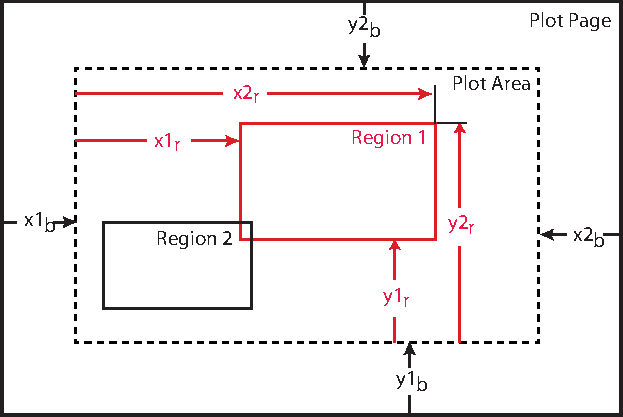
\includegraphics{plot-page.pdf}
  \caption[The plot window.]{The \vn{plot page} is the entire display window area. The \vn{plot area} 
is the region within the boarders of the \vn{plot page} within which ``\vn{regions}'' are
placed. The location of a \vn{region} is defined by four offsets with respect to the \vn{plot
area}. Regions may overlap.}
  \label{f:plot.page}
\end{figure}

%-----------------------------------------------------------------
\section{Plot Page}
\label{s:plot.page.def}

The \vn{plot page}, sometimes called the \vn{plot window}, refers to the window or the corresponding
printed graphics page where graphics are displayed. A \vn{plot page} is shown schematically in
\fig{f:plot.page}. Parameters associated with the \vn{plot page} are discussed in
\sref{s:plot.page}.  These parameters may be set in an initialization file or may be set on the \tao
command line using the \vn{set plot_page} (\sref{s:set.plot.page}) command. Examples:
\begin{example}
  set plot_page text_height = 11  ! 11 point font size
  set plot_page border%x1 = 0.2   ! Set left page border to 20% of width.
\end{example}

The size of the \vn{plot page} is set by the \vn{plot_page%size} parameter which is an array of two
numbers which set the width and height. The \vn{plot page} size can also be set when invoking \tao
using the \vn{-geometry} option (\sref{s:command.line})
\begin{example}
  > tao -lattice lat.bmad -geometry 300x500
\end{example}
This starts \tao with the \vn{plot page} size set to 300 points wide by 500 points high. It is also
sometimes convenient to start \tao without the plotting window. In this case, the \vn{-noplot} option
can be used on the startup command line. In a \tao initialization file, display of the plot window can be set
using the \vn{global%plot_on} parameter set in the \vn{tao_params} namelist (\sref{s:globals}).

In some cases, the screen resolution reported to \tao can be off. This has happened with some high
resolution displays where the reported resolution is 96 dpi when in fact the actual resolution is
much larger. In such a case, the size of the plot window created by \tao will be off. This can be
corrected by setting \vn{plot_page%size} appropriately but this in turn can create font size
problems. To avoid this problem, the environmental variable \vn{ACC_DPI_RESOLUTION} can be set to
the correct resolution before running \tao. The shell command line would be something like
\begin{example}
  > export ACC_DPI_RESOLUTION=168
\end{example}

The \vn{plot page} has a border within which \vn{regions} (\sref{s:region.def}) are defined. The area withing
the plot page border is called the \vn{plot area}

The \vn{show plot -page} (\sref{s:show.plot}) command may be used to view the page parameters.

%-----------------------------------------------------------------
\section{Region}
\label{s:region.def}

The \vn{plot area} is the area within the border of the \vn{plot page} as shown in
\fig{f:plot.page}.  In this \vn{plot area}, ``\vn{regions}'' can be defined which are invisible
rectangles where a \vn{plot} (\sref{s:plot.def}) can be placed. This is shown schematically in
\fig{f:plot.page}. Each region has a name and four numbers which specifies the location of the
region within the plot area. Regions may be defined by the user. In addition, for convenience, \tao
will define a number of regions. \tao defined regions will either begin with the letter ``\vn{r}''
or begin with the string ``\vn{layout}'' or the string ``\vn{scratch}''. Regions may overlap. How to
define regions is explained in \sref{s:plot.page}. The \vn{show plot} command will show the region
list. Example:
\begin{example}
  Tao> show plot

Plot Region         <-->  Plot                 x1    x2    y1    y2     Visible
-----------               -----------------------------------------------------
layout              <-->  lat_layout          0.00  1.00  0.00  0.15         T
r11                 <-->                      0.00  1.00  0.15  1.00
r12                 <-->                      0.00  1.00  0.58  1.00
r22                 <-->                      0.00  1.00  0.15  0.58
r13                 <-->  beta                0.00  1.00  0.72  1.00         T
r23                 <-->  dispersion          0.00  1.00  0.43  0.72         T
r33                 <-->  orbit               0.00  1.00  0.15  0.43         T
r14                 <-->                      0.00  1.00  0.79  1.00
\end{example}
The \vn{Plot} column shows what \vn{plot} (if any) is associated with the region
(\sref{s:plot.def}). The next four columns show the values of \vn{x1}, \vn{x2}, \vn{y1}, and \vn{y2}
set for the region. As shown in \Sref{s:plot.page}, \vn{x1} and \vn{x2} are the offsets from the
left \vn{plot area} edge to the left and right edges of the region. Similarly, \vn{y1} and \vn{y2}
are the offsets from the bottom edge of the \vn{plot area} to the bottom and top edges of the
region. \vn{x1} and \vn{x2} are normalized by the \vn{plot area} width and \vn{y1} and \vn{y2} are
normalized by the \vn{plot area} height so all four numbers should be in the range $[0, 1]$.  Using
the above example, the \vn{r23} region spans the full width of the \vn{plot area} (since \vn{x1} = 0
and \vn{x2} = 1), and occupies approximately the middle third vertically of the \vn{plot area}
(since \vn{y1} = 0.43 and \vn{y2} = 0.72).

The last column in the above shows if the \vn{plot} associated with the \vn{region} is
visible. Normally everything is visible. Invisibility is used in some special cases. For example,
when using a Graphical User Interface (GUI).

The \vn{set region} command can be used to set region parameters. Example:
\begin{example}
  set region r13 y1 = 0.8  ! Sets lower edge vertical position
\end{example}

%-----------------------------------------------------------------
\section{Plot}
\label{s:plot.def}

A \vn{plot} is essentially a collection of \vn{graphs}. This is shown schematically in
\fig{f:plot.plot} which shows a plot with two graph side by side.

Plots are divided into two groups. A \vn{template} plot defines how a \vn{displayed} plot is to be
constructed. That is, a \vn{template} plot defines what the associated \vn{graphs} are, defines
graph placement within the plot, etc. When a \vn{template} plot is \vn{placed} in a \vn{region},
either by using the \vn{place} command (\sref{s:place}) or by placement defined in an initialization
file (\sref{s:plot.page}), the information of the \vn{template} is copied in order to construct a
\vn{displayed} plot. A given \vn{template} plot may be placed in multiple \vn{regions} to give
multiple \vn{displayed} plots and then, using \vn{set} commands, the data displayed in each of these
plots may be manipulated separately. For example, one displayed orbit plot could show the orbit of
the \vn{model} lattice while another orbit plot could show the orbit difference between the
\vn{model} and \vn{design} lattices. When a \vn{plot} is displayed in a given \vn{region},
everything drawn is scaled to the region size.

Use the \vn{show plot} to see what displayed plots are associated with what regions. Use the
\vn{show plot -templates} command to see a list of \vn{template} plots. \tao defines a number of
default \vn{template} plots. Section~\sref{s:template} discusses how to define custom template
plots in an initialization file. Use the \vn{set plot} command (\sref{s:set.plot}) to modify either
\vn{template} or \vn{displayed} plots.

All plots have a name. A \vn{displayed} plot will inherit the same name of the \vn{template} plot it
came from. If a given \vn{template} plot is used to create multiple \vn{displayed} plots. All of
these plots will have the same name. A \vn{displayed} plot can also be referred to by using the
associated \vn{region} name. This can be used to remove ambiguity if there are multiple
\vn{displayed} plots of the same name. Additionally, a \vn{template} plot can unambiguously be
referred to by adding the prefix ``\vn{T::}'' to the plot name. Examples:
\begin{example}
  show plot           ! Show plots associated with regions
  show plot -template ! Show template plots
  place r13 orbit     ! Put orbit template into r13 region
\end{example}

Some commands, for example, the \vn{scale} command by default will ignore \vn{template} plots unless
the plot name has the \vn{T::} prefix. Other commands, for example the \vn{show plot} command, will
preferentially show displayed plot info but will show template plot info if there are no matching
displayed plots. Examples:
\begin{example}
  scale orbit -10 10    ! Scale all displayed orbit plots. Ignore template.
  scale r33 -10 10      ! Scale only plot in r33 region.
  scale T::orbit -10 10 ! Scale template orbit plot.
  show plot e_field     ! Will show displayed e_field plot info. If no
                        ! displayed plot exists, will show template info.
\end{example}

%-----------------------

\begin{figure}[bt]
  \centering
  \includegraphics[width=5.0in]{plot-plot.pdf}
  \caption[Plotting nomenclature.]
  {
A plot has a collection of graphs and a graph has a collection of curves. A graph is located within
a plot by defining the ``\vn{box}'' associated with the \vn{graph}. Illustrated here is a plot with
two graphs placed side by side.
  }
  \label{f:plot.plot}
\end{figure}

%-----------------------------------------------------------------
\section{Box}
\label{s:box.def}

To determine where a \vn{graph} is drawn with respect to the boundaries of its associated \vn{plot},
each \vn{graph} is associated with a given ``\vn{box}''. A \vn{box} is a rectangular sub-region of
the \vn{plot}. Boxes are defined by dividing the \vn{plot} into a rectangular grid and then choosing
one of the grid rectangles to be the \vn{box} associated with the \vn{graph}. The is illustrated in
\fig{f:plot.plot} where \vn{Graph 1} is associated with the \vn{box} labeled ``\vn{1,1,2,1}'' and
\vn{Graph 2} is associated with the \vn{box} labeled \vn{2,1,2,1}.  The last two digits of a
\vn{box} label (\vn{2,1} for both graphs) specify the number of rectangles the grid has horizontally
and vertically (2 horizontally, 1 vertically here). The first two digits (\vn{1,1} for \vn{graph 1}
and \vn{2,1} for \vn{graph 2}) specify the particular rectangle associated with the \vn{box} with
\vn{1,1} designating the lower left rectangle. Different \vn{graphs} do not have to use the same
grid division to select a box from.

Setting the \vn{box} for a given \vn{graph} in a \tao initialization file is covered in \sref{s:template}.
The \vn{set graph} and \vn{show graph} commands can be used to set and show the box parameters. 
Examples:
\begin{example}
  set graph myplot.g1 box = 2 1 2 2  ! Set box of graph myplot.g1
  set graph myplot.g2 box = 1 1 1 2  ! Different graphs can use different grids
                                     !  for box selection
\end{example}

%-----------------------------------------------------------------
\section{Graph}
\label{s:graph.def}

%-----------------------------------------------------------------
\subsection{Overview}
\label{s:graph.overview}

A \vn{graph} is a diagram of some sort. Most \vn{graph}s consists of horizontal and vertical axes
along with one or more \vn{curve}s. \vn{Floor_plan} (\sref{s:floor.plan}) and \vn{lat_layout}
(\sref{s:lat.layout}) \vn{graphs}, on the other hand, shows the placement in space of the lattice
elements and do not have any associated \vn{curves}.

Every \vn{plot} has at least one \vn{graph}. How many \vn{graphs} are associated with a \vn{plot}
is a matter of convenience and different \vn{graphs} of a \vn{plot} may display different types of
information. For example, it would be possible to have a single \vn{plot} contain three \vn{graphs}
and look like what is shown in \fig{f:plot.typ}. In actuality, the figure was constructed using
three \vn{plots} each one containing one \vn{graph}.

How to define \vn{graphs} when defining \vn{template} plots is given in \sref{s:template}. The
\vn{show graph} command can be used to show graph parameters. The \vn{set graph} command can
be used to modify \vn{graph} parameters.

%-----------------------------------------------------------------
\subsection{Graph Name}
\label{s:graph.name}

All graphs have a name. For example, the graph of the standard \vn{orbit} plot is simply ``\vn{g}''.
\vn{Graphs} may be referred to using the syntax:
\begin{example}
  <plot>.<graph>
\end{example}
where \vn{<plot>} is the plot name (or the \vn{region} name associated with the \vn{plot}) and
\vn{<graph>} is the graph name. If the \vn{.<graph>} ending is omitted, all graphs of the named
\vn{plot}(s) are selected. Examples:
\begin{example}
  show graph beta   ! Show info of all graphs in all the displayed beta plots.
  show graph r13.g1 ! Show info on ``g1'' graph of region r13.
\end{example}

%-----------------------------------------------------------------
\subsection{Curve Legend of a Graph}
\label{s:curve.legend}

The \vn{curve legend} is the legend identifying what curves are associated with what perimeters. In
\fig{f:plot.typ} the top two graphs have a curve legend in the upper left hand corner of the graph.
By default, the \vn{data_type} of each curve will be used as the text for that
curve's line in the legend.  This default can be changed by setting a curve's \vn{curve%legend_tex}.
Parameters that affect the curve legend are:
\begin{example}
  plot_page%legend_text_scale        ! Also affects lat_layout and floor_plan text size.      
  plot_page%curve_legend_line_len    ! tao_plot_page namelist (\sref{s:plot.page})
  plot_page%curve_legend_text_offset ! tao_plot_page namelist (\sref{s:plot.page})
  curve(N)%legend_text               ! 
  graph%curve_legend_origin          
  graph%draw_curve_legend            
\end{example}
The curve legend is distinct from the \vn{text legend} (\sref{s:text.legend}).

%-----------------------------------------------------------------
\subsection{Text Legend}
\label{s:text.legend}

The \vn{text legend} is a legend that can be setup by either the user or by \tao itself.
\tao uses the text legend in conjunction with phase space plotting or histogram displays.
The \vn{text legend} is distinct from the \vn{curve legend}. Parameters that affect the text
legend are:
\begin{example}
  graph%text_legend(:)      ! Array of strings to print
  graph%text_legend_origin  ! Position of legend.
\end{example}

%-----------------------------------------------------------------
\subsection{Graph Types}
\label{s:graph.types}

\tao defines several kinds of graphs. The \vn{graph%type} in the \vn{tao_template_graph}
(\sref{s:template}) sets the type.
\begin{description}
%
\item["data"] \Newline
``Data'' plotting is the plotting of a dependent variable on the $y$-axis vs an independent variable
on the $x$-axis. Typically the independent variable will be the longitudinal position $s$-position
as in the upper two graphs in \fig{f:plot.typ}. Also see \Sref{s:draw.ap} for an example where beam
apertures are added to the graph.

A ``\vn{data slice}'' graph is plotting one data array on the $y$-axis versus another data array on
the $x$-axis (\sref{s:graph.data.slice}). Also see \vn{parametric plotting} (\sref{s:param.plot}).

With a \vn{parametric} plot both the $x$ and $y$ values of the points on a curve are dependent
upon an independent parameter (\sref{s:param.plot}). This is similar to a \vn{data slice} plot
(\sref{s:graph.data.slice}).
%
\item["dynamic_aperture"] \Newline
A \vn{dynamic aperture} graph (\sref{s:da.plot}) draws the results from a dynamic aperture
calculation (\sref{s:da.calc}).
%
\item["floor_plan"] \Newline
A \vn{floor plan} graph shows the physical layout of the machine (\sref{s:floor.plan}). A table maps
lattice elements to a shape that is drawn (\sref{s:shapes}). The user may override the default
mapping. Besides the lattice elements. the outline of the building or tunnel that the machine is in
can be drawn (\sref{s:building.wall}).
%
\item["histogram"] \Newline
Currently \vn{histograms} (\sref{s:histogram}) are limited to displaying phase space data.
%
\item["key_table"] \Newline
The \vn{key table} displays information about variables bound to keyboard keys \sref{s:key.bind}.
Key bindings are used in \vn{single mode}.
%
\item["lat_layout"] \Newline
A \vn{lattice layout} graph displays the lattice elements as a series of shapes as a function of the
longitudinal position $s$ (\sref{s:lat.layout}). The lowest graph in \fig{f:plot.typ} is an example
of a \vn{lattice layout}.  A table maps lattice elements to a shape that is drawn (\sref{s:shapes}).
The user may override the default mapping.
%
\item["phase_space"] \Newline
A \vn{phase space graph} (\sref{s:phase.space}) displays particle positions in phase space after
a beam of particles has been tracked (\sref{s:beam.init}).
%
\item["wave.0", "wave.a", "wave.b"] \Newline
Wave analysis plotting (\sref{c:wave}).
%
\end{description}

\begin{figure}[b]
  \centering
  \includegraphics[width=5.0in]{plot-axes.pdf}
  \caption[Plot axes.]
{A data graph has three axes called \vn{x} (bottom edge), \vn{y} (left edge), and \vn{y2} (right edge).}
  \label{f:plot.axes}
\end{figure}

%-----------------------------------------------------------------
\subsection{Graph Axes}
\label{s:axes}

Data graphs (\sref{s:graph.types}) have three axes as shown in \fig{f:plot.axes}. The bottom axis is
called \vn{x}, and the left and right axes are called \vn{y} and \vn{y2} respectively. The
\vn{qp_axis_struct} structure (\sref{s:qp.axis}) is used to store axis parameters which can be
accessed via the \vn{graph%x}, \vn{graph%y}, and \vn{graph%y2} components in the
\vn{tao_template_graph} namelist (\sref{s:template}) or by using the \vn{set graph} command
(\sref{s:set.graph}.

The \vn{scale} command (\sref{s:scale}) can be used to set the vertical axes. The \vn{x_scale}
(\sref{s:x.scale}) command can be used to set the horizontal axis.

Normally there is only one vertical scale for a graph and this is associated with the \vn{y}
axis. However, if any curve of a given graph has \vn{curve%use_y2} set to \vn{True} then the \vn{y2}
axis will have an independent second scale. In this case, the \vn{y2} axis numbers will be
drawn. Notice that simply giving the \vn{y2} axis a label does {\em not} make the \vn{y2} axis scale
independent of the \vn{y} axis scale.

The following \vn{tao_plot_page} namelist (\sref{s:plot.page}) parameters affect the drawing of the axes:
\begin{example}
  text_height = 12              ! In points. Scales the height of all text
  axis_number_text_scale = 0.9  ! Relative to text_height
  axis_label_text_scale = 1.0   ! Relative to text_height
\end{example}

%-----------------------------------------------------------------
\section{Curve}
\label{s:curve.def}

%-----------------------------------------------------------------
\subsection{Overview}
\label{s:curve.overview}

A \vn{curve} is a data set to be displayed within a \vn{graph}. For example, a \vn{curve} may be the
beta function of the \vn{model} lattice. \vn{Curves} have an associated set of points at which a
symbol can be drawn. A curve also can have an associated curved line that can be drawn. For example,
in \fig{f:plot.typ} only the line is drawn with the two curves of the beta plot while both symbols
and line are drawn for the two curves of the orbit plot (here the data points where symbols are
drawn are the orbit at the edges of the lattice elements).

Some \vn{graphs} do not have any associated curves. For example, a \vn{lat_layout} graph does not
have associated curves.

How to define \vn{curves} when defining \vn{template} plots is given in \sref{s:template}. The
\vn{show curve} command can be used to show curve parameters. The \vn{set curve} command can
be used to modify \vn{curve} parameters.

%-----------------------------------------------------------------
\subsection{Curve Name}
\label{s:curve.name}

All curves have a name. \vn{Curves} may be referred to using the syntax:
\begin{example}
  <plot>.<graph>.<curve>
\end{example}
where \vn{<plot>} is the plot (or \vn{region}) name, \vn{<graph>} is the graph name and \vn{<curve>}
is the curve name. If the \vn{.<curve>} ending is omitted, all curves of the named \vn{graph}(s) are
selected. If the \vn{.<graph>.<curve>} ending is omitted, all curves of the named \vn{plot}(s) are
selected. Examples:
\begin{example}
  show curve beta   ! Show info of all curves in all the displayed beta plots.
  show curve r13.g1 ! Show info on curves in ``g1'' graph of region r13.
  set graph orbit.g curve_legend_origin = 0.1 -0.2 "%BOX/LT"  ! Set curve legend origin
\end{example}
The last example sets the \vn{curve legend} (\sref{s:template}) of the graph so that the curve
legend of the graph is drawn with respect to the left top corner of the box.

%-----------------------------------------------------------------
\subsection{Curve Line}
\label{s:curve.line}

Each curve may have an associated line that is drawn. The line may be a set of line segments
connecting curve symbol points (\sref{s:curve.sym}) or may be a ``smooth'' curve calculated by
evaluating the curve at a number of points. 

\vn{curve%draw_line} determines whether a curve is drawn through the data point symbols. The
thickness, style (solid, dashed, etc.), and color of the line can be controlled by setting
\vn{curve%line}. If \vn{plot%x_axis_type} is \vn{"s"}, and \vn{curve%component} does not contain
\vn{"meas"} or \vn{"ref"}, \tao will attempt to calculate intermediate values in order to draw a
smooth, accurate curve is drawn. Occasionally, this process is too slow or not desired for other
reasons so setting \vn{curve%smooth_line_calc} to False will prevent this calculation and the curve
will be drawn as a series of lines connecting the symbol points. The default of
\vn{curve%smooth_line_calc} is True. Use the \vn{set curve} command (\sref{s:set}) to toggle the
drawing of lines. Alternatively, the \vn{-disable_smooth_line_calc} switch can be used on the
command line (\sref{s:command.line}) or the global variable \vn{global%disable_smooth_line_calc} can
be set in the \tao initialization file (\sref{s:globals}).

The number of points to evaluate at when constructing a smoothed line is set by
\vn{plot_page%n_curve_pts} in the \vn{tao_plot_page} namelist (\sref{s:plot.page}) or by using the
\vn{set plot_page} command (\sref{s:set.plot.page}). To override this value for a particular plot
the \vn{plot%n_curve_pts} parameter can be set in the \vn{tao_template_plot} namelist or using the
\vn{set plot} command (\sref{s:set.plot}). More evaluation points may give a more accurate curve at
the expense of computation time.

%-----------------------------------------------------------------
\subsection{Curve Symbol}
\label{s:curve.sym}

\vn{curve%draw_symbols} determines whether a symbol is drawn at the data points. The size, shape and
color of the symbols is determined by \vn{curve%symbol}. A given symbol point that is drawn has
three numbers attached to it: The $(x, y)$ position on the graph and an index number to help
identify it. The index number of a particular symbol is the index of the datum or variable
corresponding the symbol in the \vn{d1_data} or \vn{v1_var} array. These three numbers can be
printed using the \vn{show curve -symbol} command (\sref{s:show}).  \vn{curve%draw_symbol_index}
determines whether the index number is printed besides the symbol. Use the \vn{set curve} command
(\sref{s:set}) to toggle the drawing of symbols. The default value for \vn{curve%draw_symbol} is
False if \vn{plot%x_axis_type} is \vn{"s"}, \vn{"curve"}, \vn{"lat"}, or \vn{"var"} and True
otherwise. The default \vn{curve%draw_symbol_index} is always False.

The \vn{graph%draw_only_good_user_data_or_vars} logical determines whether datums
(\sref{s:init.data}) or variables (\sref{s:init.var}) with a \vn{good_user} component set to
\vn{False} are drawn. The default is to not draw them which means that data or variables not used in
an optimization are not drawn.

%-----------------------------------------------------------------
\subsection{Curve Component}
\label{s:curve.comp}

A ``\vn{data}'' graph (\sref{s:graph.types}) is used to draw lattice parameters such as orbits, or
\tao data (\sref{c:data}), or variable values such as quadrupole strengths. The data values will
depend upon where the data comes from. This is determined, in part, by the setting of the
\vn{component} parameter in the \vn{tao_template_graph} namelist (\sref{s:template}).  The
\vn{component} may be one of:
\index{model}\index{design}\index{base}\index{meas}\index{ref}
\begin{example}
  "model"             ! model values. Default.
  "design"            ! design values.
  "base"              ! Base values
  "meas"              ! data values.
  "ref"               ! reference data values.
  "beam_chamber_wall" ! Beam chamber wall
\end{example}
Additionally, \vn{component} may be set to plot a linear combination of the above. For
example:
\begin{example}
  &tao_template_graph
    curve(2)%component = "model - design"
    ...
\end{example}
This will plot the difference between the \vn{model} and \vn{design} values. 
The default value of \vn{%component} is \vn{"model"}.

%-----------------------------------------------------------------
\subsection{Curve Data Source}
\label{s:curve.source}

\index{data}\index{var}\index{calculation}
\index{curve!data_source}
The \vn{data_source} parameter of a curve is the type of information for the source of the data points.
\vn{data_source} must be one of:
\begin{example}
  "data"              ! A d1_data array is the source of the curve points.
  "var"               ! A v1_var array is the source of the curve points.
  "lat" (Default)     ! The curve points are computed directly from the lattice.
  "beam"              ! The curve points are computed from tracking a beam of particles.
  "multi_turn_orbit"  ! Computation is from multi-turn tracking. 
\end{example}
The default for \vn{data_source} is \vn{"lat"}. With \vn{data_source} set to "\vn{data}",
the values of the curve points come from the \vn{d1_data} array structure named by
the curve's \vn{data_type} parameter (\sref{s:curve.type}).

If \vn{data_source} is set to \vn{var}, the values of the curve points come from a \vn{v1_var}
array structure. If it is set to \vn{lat} the curve data points are calculated from the lattice
without regard to any data structures. \vn{data_source} can be set to \vn{beam} when tracking
beams of particles. In this case, the curve points are calculated from the tracking. With \vn{beam},
the particular bunch that the data is extracted from can be specified via \vn{ix_bunch}. The
default is \vn{0} which combines all the bunches of the beam for the calculation.

Used in conjunction with \vn{data_type} and \vn{component} (\sref{s:curve.comp}). For
example (\sref{s:curve.source}), a curve of the orbit with \vn{data_source} set to \vn{"beam"}
would use the beam centroid computations. If the \vn{data_source} was set to \vn{"lat"} the
computed orbit using single particle tracking is used.

Example: With \vn{data_type} set to \vn{beta.x}, the setting of \vn{data_source} to
\vn{lat} gives the beta as calculated from the lattice and \vn{beam} gives the beta as calculated
from the shape of the beam.

%-----------------------------------------------------------------
\subsection{Curve Data Type}
\label{s:curve.type}

The \vn{data_type} of a curve specifies what is being plotted. What the valid settings for \vn{data_type}
are depends upon the type of graph (\sref{s:graph.types}). 
\begin{description}
%
\item[graph\%type = "data", or "histogram"] \Newline
Valid settings for \vn{data_type} are any \tao datum type (\sref{s:data.table}), \tao variable
(\sref{c:var}), and the following electric and magnetic field components:
\begin{example}
  b0_field.x,  b0_field.y,  b0_field.z,  b0_curl.x,  b0_curl.y,  b0_curl.z,  b0_div
  e0_field.x,  e0_field.y,  e0_field.z,  e0_curl.x,  e0_curl.y,  e0_curl.z,  e0_div
\end{example}
The field data types with names starting with ``b_'' and ``e_'' evaluate the field along the single
particle trajectory while the field data types with names starting with ``b0_'' and ``e0_'' are evaluated
along a constant transverse position specified by the curve's \vn{orbit} parameter.
%
\item[graph\%type = "dynamic_aperture"] \Newline
Valid settings for \vn{data_type} are:
\begin{example}
  "beam_ellipse"
  "dynamic_aperture"
\end{example}
%
\item[graph\%type = floor_plan", "lat_layout", or "key_table"] \Newline
There are not curves associated with these graph types.
%
\item[graph\%type = "phase_space"] \Newline
Valid settings for \vn{data_type} are:
\begin{example}
  "x",  "px",  "y",  "py",  "z",  "pz",
  "intensity",  "intensity_x",  "intensity_y"     ! Photon intensity
  "phase_x", "phase_y"                            ! Photon coherent phase
\end{example}
%
\end{description}

 For example, with \vn{graph%type} set to
\vn{dynamic_aperture} the 




Thus in the above example the curve point values are obtained from
\vn{orbit.x} data. To be valid the data structure named by \vn{data_type} must be set up in an
initialization file. If not given, the default \vn{data_type} is
\begin{example}
  <plot%name>.<graph%name>
\end{example}

%-----------------------------------------------------------------
\section{Quick_Plot Plotting}
\label{s:quick.plot}

\vn{Quick_plot} is a software library developed for \bmad and \tao for graphics plotting.

%-----------------------------------------------------------------
\subsection{Length and Position Units}
\label{s:qp.units}

Positions and lengths with \vn{quick_plot} generally have an associated ``\vn{units}'' string which determines how
$(x, y)$ positions or $(dx, dy)$ lengths are to be interpreted. 
The syntax of the \vn{units} parameter is:
\begin{example}
  "unit_type/ref_object/corner"
\end{example}
A \vn{units} string has a \vn{unit_type}, \vn{ref_object} and \vn{corner} components separated by slashes ``/''.

The \vn{unit_type} component is the type of units which can be one of:
\begin{example}
   "%"       - Percent.
   "DATA"    - Data units associated with a graph.
   "MM"      - millimeters.
   "INCH"    - Inches.
   "POINTS"  - Printers points (72 points = 1 inch, 1 pt ~ 1 pixel).
\end{example}
Note: If \vn{unit_type} is set to \vn{"DATA"}, \vn{ref_object}, if present, must be \vn{"GRAPH"} and
\vn{corner}, if present, must be \vn{"LB"}.

The \vn{ref_object} component is a reference object which can be one of:
\begin{example}
   "PAGE"  -- Relative to the plot display window.
   "BOX"   -- Relative to the box the graph is associated with.
   "GRAPH" -- Relative to the graph rectangle.
\end{example}
The \vn{ref_object} component is optional if a relative length is being specified and the
\vn{unit_type} is anything other than \vn, the slash between
the \vn{unit_type} and the \vn{ref_object} may be omitted.

Note: The \vn{"PAGE"} reference is the entire \vn{plot page} and not the \vn{plot area}. The
\vn{plot area} is only used for defining the placement of \vn{regions}.

The \vn{corner} component is the origin location of the reference object.
\vn{corner} can be one of:
\begin{example}
   "LB" -- Left Bottom of reference object. Default.
   "LT" -- Left Top.
   "RB" -- Right Bottom.
   "RT" -- Right Top.
\end{example}
The \vn{ref_object} component is optional if a relative length is being specified.

Examples:
\begin{example}
  "DATA"          -- Equivalent to "DATA/GRAPH/LB"
  "DATA/GRAPH/LB" -- Same as above.
  "DATA/BOX/RT"   -- ILLEGAL: DATA must always go with GRAPH/LB.
  "%/PAGE/LT"     -- Equivalent to "%PAGE/LT"
  "%PAGE/LT"      -- Percentage of page so (0.0, 1.0) = RT of page.
  "%BOX"          -- Percentage of box so (1.0, 1.0) = RT of box.
  "INCH/PAGE"     -- Inches from LB of page. Equivalent to "INCH/PAGE/LB"
\end{example}

Units can be set in an initialization file or with the \vn{set} command. Example:
\begin{example}
  set plot_page title%units = '%PAGE'
\end{example}

%-----------------------------------------------------------------
\subsection{Text Justification Units}
\label{s:qp.str.just}

Text justification units is a two character string that sets where a line of text is to be printed
with respect to the text $(x, y)$ position.
The first character of the justification string gives the horizontal alignment:
\begin{example}
   "L" -- Left justify
   "C" -- Center justify
   "R" -- Right justify
\end{example}
The second character of the justification string gives the vertical alignment:
\begin{example}
   "B" -- Bottom justify
   "C" -- Center justify
   "T" -- Top justify
\end{example}

Example:
\begin{example}
  plot_page%title%justify = 'CC'
\end{example}

%-----------------------------------------------------------------
\subsection{qp_point_struct}
\label{s:qp.point}

\vn{QuickPlot} defines a number of structures to parameterize such things like line and symbol
properties.

The \vn{qp_point_struct} defines where a point is:
\begin{example}
  type qp_point_struct:
    x     = <real>     ! Horizontal offset of point from fiducial point
    y     = <real>     ! Vertical offset of point from fiducial point
    units = "<units>"  ! Units of x \& y (\sref{s:qp.units}).
\end{example}
Example:
\begin{example}
  graph%curve_legend_origin = 5.0, -2.0, "POINTS/GRAPH/LT"
\end{example}
In this example the fiducial point the left-top point on the graph rectangle. The
\vn{curve_legend_origin} is positioned 5.0 points horizontally to the left and 2.0 points vertically
downward from this fiducial point.

%-----------------------------------------------------------------
\subsection{qp_line_struct}
\label{s:qp.line}

The parameters associated with data lines drawn in a graph are contained in the \vn{qp_line_struct}:
\begin{example}
  type qp_line_struct:
    width    = <integer>  ! Default = 1
    color    = <string>   ! Default = "black" (\sref{s:qp.color}).
    pattern  = <string>   ! Default = "solid" (\sref{s:qp.line.pat}).
\end{example}

%-----------------------------------------------------------------
\subsection{Symbols}
\label{s:qp.sym}

The parameters associated with symbols that are drawn are contained in the \vn{qp_symbol_struct}:
\begin{example}
  type qp_symbol_struct:
    type          = <string>  ! Default = "dot"
    height        = <real>    ! Size in points. Default = 10
    color         = <string>  ! Default = "black" (\sref{s:qp.color})
    fill_pattern  = <string>  ! Default = "solid_fill"
    line_width    = <integer> ! Default = 1.
\end{example}

\begin{table}
  \centering
  \includegraphics[width=5in]{plot-syms.pdf}
  \caption{Plotting Symbols.}
  \label{t:plot.syms}
\end{table}

The symbol types are:
\begin{example}
  square                 triangle                    square_concave              
  dot                    circle_plus                 diamond                     
  plus                   circle_dot                  star5                       
  times                  square_filled               triangle_filled           
  circle                 circle_filled               red_cross                 
  x                      star5_filled                star_of_david             
\end{example}
These symbols are illustrated in Table~\ref{t:plot.syms}. Symbol type names are case insensitive.

%-----------------------------------------------------------------
\subsection{qp_axis_struct}
\label{s:qp.axis}

The \vn{qp_axis_struct} structure defines the properties of a graph axis
\begin{example}
  type qp_axis_struct::
    label             = "<string>" ! Axis label string.
    min               = <real>     ! Min is the left or bottom axis number.
    max               = <real>     ! Max is the right or top axis number.
    number_offset     = <real>     ! Offset from axis line in inches.
    label_offset      = <real>     ! Offset from numbers in inches.
    major_tick_len    = <real>     ! Major tick length in inches.
    minor_tick_len    = <real>     ! Minor tick length in inches.
    label_color       = <string>   ! Color of the label string (\sref{s:qp.color})
    major_div         = <integer>  ! Number of major divisions
    major_div_nominal = <integer>  ! Major divisions nominal value.
    minor_div         = <integer>  ! Minor divisions. 0 = Tao will choose.
    minor_div_max     = <integer>  ! Max minor div number if Tao chooses.
    places            = <integer>  ! Number of digits to print
    type              = <string>   ! Axis type: "LINEAR" or "LOG".
    bounds            = <string>   ! Axis bounds: "GENERAL", "ZERO_AT_END", etc.
    tick_side         = <integer>  ! 1 = draw to the inside, 0 = both, -1 = outside.
    number_side       = <integer>  ! 1 = draw to the inside, -1 = outside.
    draw_label        = <logical>  ! Draw the label string
    draw_numbers      = <logical>  ! Draw the numbers.
\end{example}

The \vn{%bounds} parameter sets how the axes min and max values are calculated when plots are initially
instantiated and when \vn{scale}, \vn{x_scale}, and \vn{xy_scale} commands are used. Possible settings
are:
\begin{example}
  "ZERO_AT_END"      ! Min or max value is set to zero.
  "ZERO_SYMMETRIC"   ! Min and max chosen so that max = -min.
  "GENERAL"          ! No restrictions (default).
  "EXACT"            ! The User min/max is used.
\end{example}
If input min and max values are specified by the User, \tao will take the specified values as the starting
point to find ``nice'' min and max values to use. For example, with the command
\begin{example}
  scale all 0 19
\end{example}
and with \vn{bounds} set to \vn{"GENERAL"}, the min and max values will be set to 0 and 20. The exception is when
\vn{bounds} is set to \vn{"EXACT"}. In this case the User supplied min and max values will be used as is.

Examples:
\begin{example}
Tao> set graph r13 y%bounds = "zero_at_end"
Tao> scale r13 200 280   ! Graph bounds set to [0, 300]

Tao> set graph r13 y%bounds = "zero_symmetric"
Tao> scale r13 200 280   ! Graph bounds set to [-300, 300]

Tao> set graph r13 y%bounds = "general"
Tao> scale r13 20 190    ! Graph bounds set to [0, 200]

Tao> set graph r13 y2%bounds = "exact"
Tao> scale r13 -y2 20 190    ! Y2 graph bounds set to [20, 190]
\end{example}

Both \vn{major_div} and \vn{major_div_nominal} set the number of major divisions in the plot. The
difference between the two is that with \vn{major_div} set positive and \vn{major_div_nominal} set
zero or negative, the number of major divisions is fixed at the value of \vn{major_div}. With
\vn{major_div_nominal} positive, the value of \vn{major_div} is ignored, and the number of major
divisions will be chosen to be a ``nice'' value near the value of \vn{major_div_nominal}. If neither
\vn{major_div} nor \vn{major_div_nominal} is set positive, a value will be chosen for
\vn{major_div_nominal} by \tao. If you are unsure which to set, it is recommended that
\vn{major_div_nominal} be used.

The \vn{places} parameter set the number of places to display a number. \tao will automatically
calculate this number and it is not user settable.

The \vn{label} parameter may include Greek letters, subscripts, superscripts, and special characters.
Encoding for these are given in Table~\ref{t:plot.escape}. 

%-----------------------------------------------------------------
\subsection{qp_legend_struct}
\label{s:qp.legend.str}

The parameters associated with drawing a curve legend (\sref{s:plot.def}) are contained in the parameter
\vn{plot_page%curve_legend} (\sref{s:plot.page}). This parameter is an instance of a \vn{qp_legend_struct}
which has the structure:
\begin{example}
  type qp_legend_struct
    type (qp_point_struct) origin  ! Location of legend.
    row_spacing = <real>           ! Spacing between rows. Default = 1.0.
    line_length = <real>           ! Length of the line in points.
    text_offset = <real>           ! Horizontal offset in points between the line and the text.
    logical draw_line = <logic>    ! Draw lines?
    logical draw_symbol = <logic>  ! Draw symbols?
    logical draw_text = <logic>    ! Draw text?
  end type
\end{example}

%-----------------------------------------------------------------
\subsection{String Escape Sequences}
\label{s:qp.str}

\begin{table}[tb]
\begin{tabular}{ll} \toprule
{\B}u       & Start a superscript or end a subscript \\[0.3ex]
{\B}d       & Start a subscript or end a superscript.
              {\B}u and {\B}d must always be used in pairs \\[0.3ex]
{\B}b       & Backspace (i.e., do not advance text pointer  
               after plotting the previous character) \\[0.3ex]
{\B}fn      & Switch to Normal font (1)       \\[0.3ex]
{\B}fr      & Switch to Roman font (2)        \\[0.3ex]
{\B}fi      & Switch to Italic font (3)       \\[0.3ex]
{\B}fs      & Switch to Script font (4)       \\[0.3ex]
{\B}{\B}    & Backslash character (\B)        \\[0.3ex]
{\B}x       & Multiplication sign ($\times$)  \\[0.3ex]
{\B}.       & Centered dot ($\cdot$)          \\[0.3ex]
{\B}A       & Angstrom symbol (\AA)         \\[0.3ex]
{\B}gx      & Greek letter corresponding to roman letter x. See Table~\ref{t:greek}. \\[0.3ex]
{\B}mN {\B}mNN & Graph marker number \vn{N} or \vn{NN} (1-31) \\[1ex]
{\B}(NNNN)  & 
\parbox{5.2in} {Character number NNNN (1 to 4 decimal digits) from the Hershey character set which
includes a number of special characters including mathematical, musical, astronomical, and
cartographical symbols.} \\ \bottomrule
\end{tabular}
\caption{Escape Sequences for Labels.}
\label{t:plot.escape}
\end{table}

Table~\ref{t:greek} shows how the character string \vn{"{\B}g<r>"}, where \vn{"<r>"} 
is a Roman letter, map onto the Greek character set.
\begin{table}[tb]
  \centering
  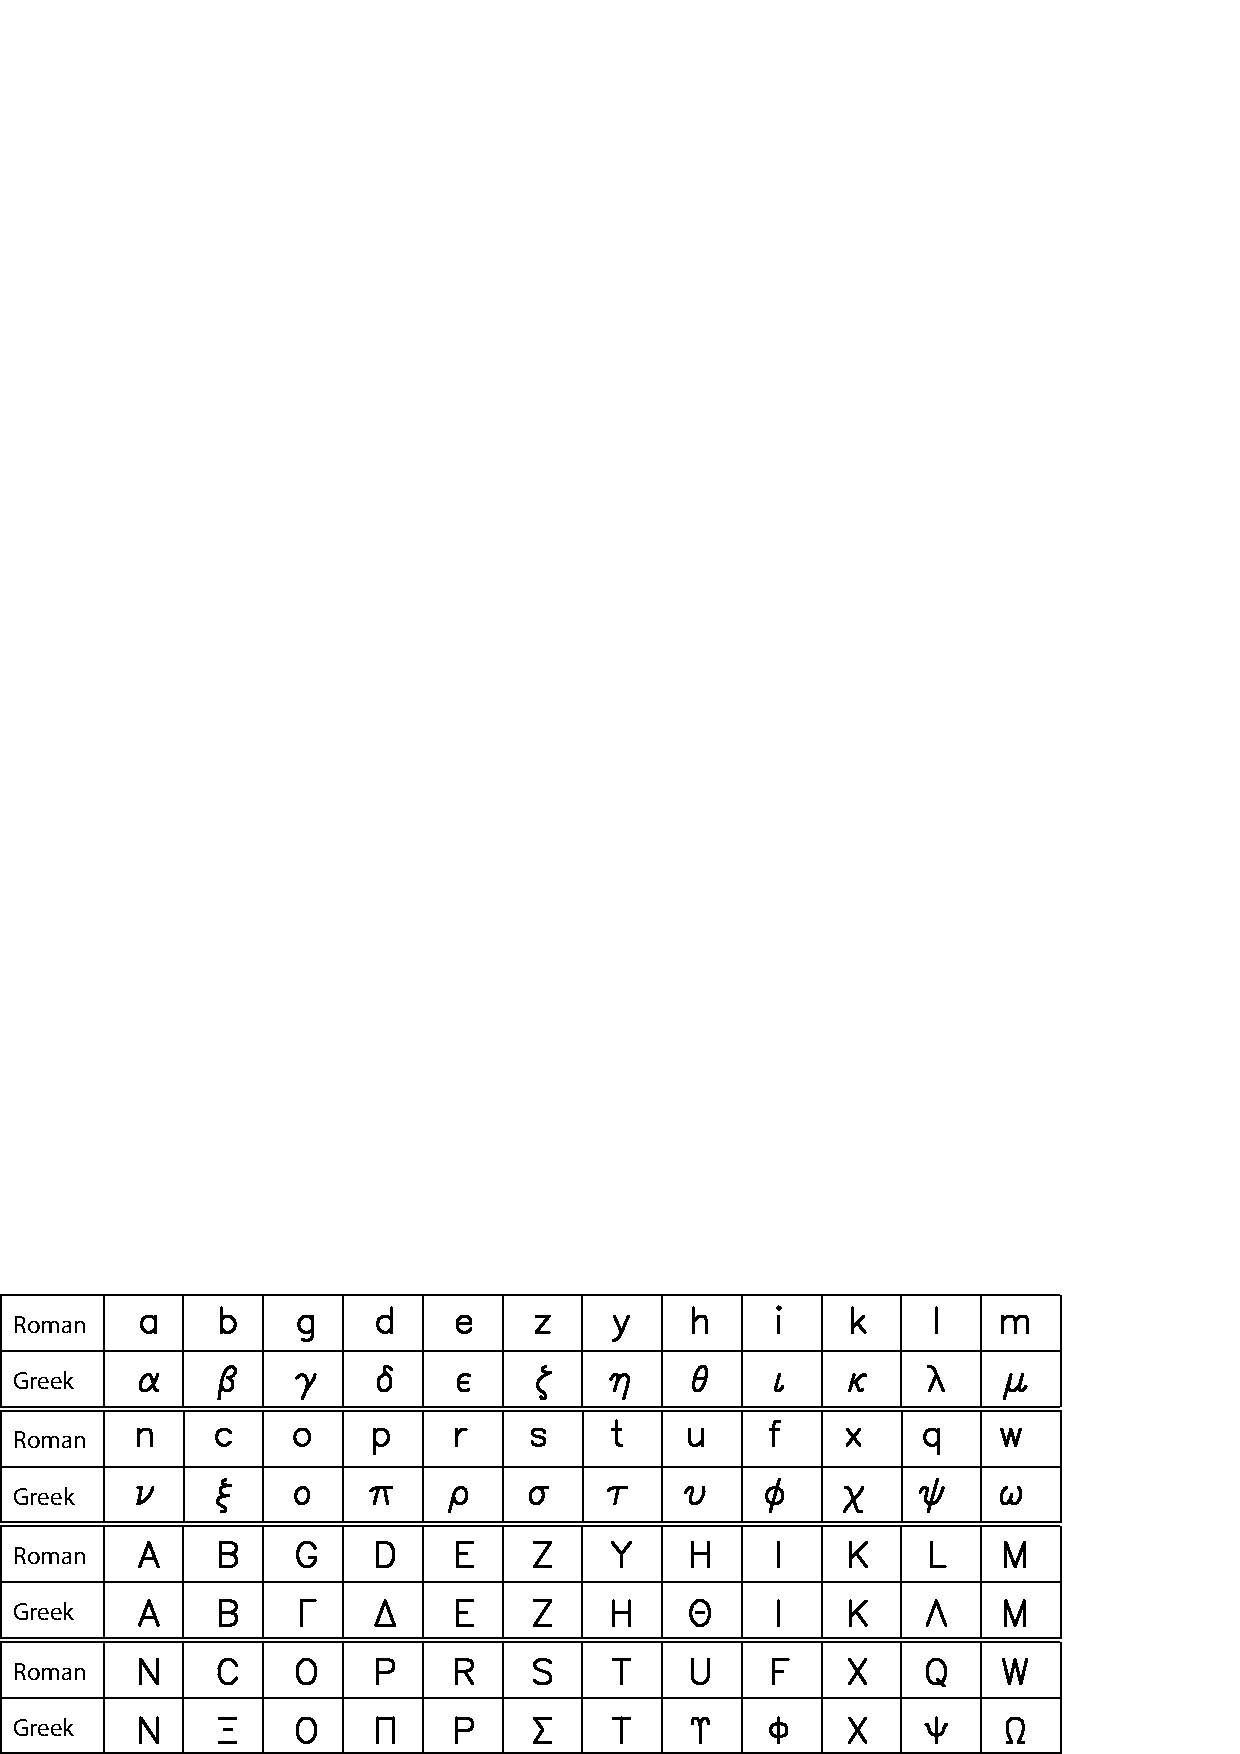
\includegraphics[width=5.0in]{greek.pdf}
  \caption[Roman to Greek Character Conversion]{Conversion for the string 
\vn{"{\B}g<r>"} where \vn{"<r>"} is a Roman character to the corresponding 
Greek character.}
\label{t:greek}
\end{table}

%-----------------------------------------------------------------
\subsection{Color Names}
\label{s:qp.color}

Possible settings for color parameters are:
\begin{example}
  White   (actually the background color)       Orange          
  Black   (actually the foreground color)       Yellow_Green    
  Red                                           Light_Green         
  Green                                         Navy_Blue       
  Blue                                          Purple          
  Cyan                                          Reddish_Purple  
  Magenta                                       Dark_Grey        
  Yellow                                        Light_Grey       
\end{example}
Color names are case insensitive.

%-----------------------------------------------------------------
\subsection{Line Pattern Names}
\label{s:qp.line.pat}

Possible settings for line patterns are:
\begin{example}
  solid      ! Solid line                 dotted     ! Dotted line             
  dashed     ! Dashed line                dash_dot3  ! Dash--dot--dot--dot line
  dash_dot   ! Dash--dot line
\end{example}
Pattern names are case insensitive.

%-----------------------------------------------------------------
\subsection{Fill Pattern Names}
\label{s:qp.fill.pat}

Possible fill pattern settings for symbols are:
\begin{example}
  solid_fill                    hatched           
  no_fill                       cross_hatched     
\end{example}
Fill pattern names are case insensitive.


\chapter{Bmad Library Subroutine List}

Below are a list of \bmad and sim_utils routines sorted by their
functionality.  Use the \vn{getf} and \vn{listf} (\sref{s:getf}) 
scripts for more information on individual routines.
This list includes low level routines that are not generally used in
writing code for a program but may be useful in certain unique
situations.  Excluded from the list are very low level routines that are
solely meant for \bmad internal use.

\toffset
\begin{center}
\begin{tabular}{|l|l|} \hline
{\em Routine Type} & {\em Section} \\ \hline
  Beam: Low Level Routines                    & \ref{r:low.beam}       \\ \hline
  Beam: Tracking and Manipulation             & \ref{r:beam}           \\ \hline
  Branch Handling                             & \ref{r:branch}         \\ \hline
  \cpp Interface                              & \ref{r:cpp}            \\ \hline
  Coherent Synchrotron Radiation (CSR)        & \ref{r:csr}            \\ \hline
  Collective Effects                          & \ref{r:collective}     \\ \hline
  Electro-Magnetic Fields                     & \ref{r:em.fields}      \\ \hline
  Inter-Beam Scattering (IBS)                 & \ref{r:ibs}            \\ \hline
  Lattice: Element Informational              & \ref{r:info}           \\ \hline
  Lattice: Element Manipulation               & \ref{r:elem}           \\ \hline
  Lattice: Geometry                           & \ref{r:geom}           \\ \hline
  Lattice: Low Level Stuff                    & \ref{r:low.help}       \\ \hline
  Lattice: Manipulation                       & \ref{r:trans}          \\ \hline
  Lattice: Miscellaneous                      & \ref{r:misc.help}      \\ \hline
  Lattice: Reading and Writing Files          & \ref{r:read}           \\ \hline
  Matrices                                    & \ref{r:mat}            \\ \hline
  Matrix: Low Level Routines                  & \ref{r:low.mat}        \\ \hline
  Measurement Simulation Routines             & \ref{r:meas}           \\ \hline
  Multipass                                   & \ref{r:multipass}      \\ \hline
  Multipoles                                  & \ref{r:multipoles}     \\ \hline
  sim_utils routines                          & \ref{r:sim.utils}       \\ \hline
  Optimizers (Nonlinear)                      & \ref{r:opti}           \\ \hline
  Overload Equal Sign                         & \ref{r:equal}          \\ \hline
  Particle Coordinate Stuff                   & \ref{r:coord}          \\ \hline
  PTC Interface                               & \ref{r:ptc}            \\ \hline
  Quick Plot                                  & \ref{r:qp}             \\ \hline
  Spin                                        & \ref{r:spin}           \\ \hline
  Transfer Maps: Routines Called by MAKE_MAT6 & \ref{r:mat6}           \\ \hline
  Transfer Maps: Taylor Maps                  & \ref{r:taylor}         \\ \hline
  Tracking and Closed Orbit                   & \ref{r:track}          \\ \hline
  Tracking: Low Level Routines                & \ref{r:low.track}      \\ \hline
  Tracking: Macroparticle                     & \ref{r:macro}          \\ \hline
  Tracking: Mad Routines                      & \ref{r:mad}            \\ \hline
  Tracking: Routines Called by TRACK1         & \ref{r:track1}         \\ \hline
  Twiss and Other Calculations                & \ref{r:twiss}          \\ \hline
  Twiss: 6-Dimensional                        & \ref{r:twiss6}         \\ \hline
  Wake Fields                                 & \ref{r:wake}           \\ \hline
  Deprecated                                  & \ref{r:deprecated}     \\ \hline
\end{tabular}
\end{center}
\toffset

%------------------------------------------------------------------------
\section{Beam: Low Level Routines}
\label{r:low.beam}

The following helper routines are generally not useful for general use.

\begin{description}

\index{Routine!add_sr_long_wake}
\item[add_sr_long_wake (ele, bunch, num_in_front, follower)] \Newline 
Adds the longitudinal wake for all particles in front of the follower.

\index{Routine!beam_equal_beam}
\item[beam_equal_beam (beam1, beam2)] \Newline 
Subroutine to set one particle beam equal to another taking care of
pointers so that they don't all point to the same place.

\index{Routine!calc_bunch_params_slice}
\item[calc_bunch_params_slice (bunch, ele, params, plane, slice_center, slice_spread)] \Newline 
Finds all bunch parameters for a slice through the beam distribution.

\index{Routine!find_bunch_sigma_matrix}
\item[find_bunch_sigma_matrix (particle, ave, sigma)] \Newline 
Routine to find the sigma matrix elements of a particle distribution.

\index{Routine!init_spin_distribution}
\item[init_spin_distribution (beam_init, bunch)] \Newline 
Initializes a spin distribution according to init_beam\%spin

\index{Routine!order_particles_in_z}
\item[order_particles_in_z (bunch)] \Newline 
Subroutine to order the particles longitudinally 
The ordering uses the centroid of the particles:

\index{Routine!rest_energy}
\item[rest_energy (particle) result (energy)] \Newline 
Routine to return the rest energy in eV of a particle.

\index{Routine!track1_beam}
\item[track1_beam (beam_start, lat, ix_ele, beam_end, err)] \Newline 
Subroutine to track a beam of particles through a single element.
Overloaded by \vn{track1_beam}.

\index{Routine!track1_bunch}
\item[track1_bunch (bunch_start, lat, ix_ele, bunch_end, err)] \Newline 
Subroutine to track a bunch of particles through an element.

\index{Routine!track1_sr_wake}
\item[track1_sr_wake (bunch, ele)] \Newline 
Subroutine to apply the short range wake fields to a bunch. 

\index{Routine!track1_lr_wake}
\item[track1_lr_wake (bunch, ele)] \Newline 
Subroutine to put in the long-range wakes for particle tracking.

\index{Routine!track1_particle}
\item[track1_particle (start, ele, param, end)] \Newline 
Subroutine to track a particle through an element.

\end{description}

%------------------------------------------------------------------------
\section{Beam: Tracking and Manipulation}
\label{r:beam}    
\index{beam tracking!list of routines}

See \sref{s:part.track} for a discussion of using a collection of particles to simulate
a bunch.

\begin{description}

\index{Routine!angle_to_canonical_coords}
\item[angle_to_canonical_coords (particle, energy0)] \Newline 
Subroutine to convert particle coords from 
    (x, x', y, y', z, E)

\index{Routine!calc_bunch_params}
\item[calc_bunch_params (bunch, ele, params)] \Newline 
Finds all bunch parameters defined in bunch_params_struct, both normal-mode
and projected

\index{Routine!calc_bunch_params_slice}
\item[calc_bunch_params (bunch, ele, params, plane, slice_center, slice_spread)] \Newline 
Finds all bunch parameters for a slice through the beam distribution.

\index{Routine!canonical_to_angle_coords}
\item[canonical_to_angle_coords (particle, energy0)] \Newline 
Subroutine to convert particle coords from 
    (x, px, y, py, z, pz)

\index{Routine!init_beam_distribution}
\item[init_beam_distribution (ele, beam_init, beam)] \Newline 
Subroutine to initialize a distribution of particles matched to
the Twiss parameters, centroid position, and Energy - z correlation

\index{Routine!ion_kick}
\item[ion_kick(x, y, x_kicker, y_kicker, s_kicker)] \Newline 
    subroutine to return the kick felt by an ion due to the
    passage of a bunch. Can also be used for beam-beam simulations.

\index{Routine!reallocate_beam}
\item[reallocate_beam (beam, n_bunch, n_particle)] \Newline 
Subroutine to reallocate memory within a beam_struct.

\index{Routine!track1_bunch_custom}
\item[track1_bunch_custom (bunch_start, lat, ix_ele, bunch_end)] \Newline 
Dummy routine for custom bunch tracking. 

\index{Routine!track_beam}
\item[track_beam (lat, beam, ix1, ix2)] \Newline 
     Subroutine to track a beam of macroparticles from the end of
     lat\%ele(ix1) Through to the end of lat\%ele(ix2).

\end{description}

%------------------------------------------------------------------------
\section{Branch Handling Routines}
\label{r:branch}

\begin{description}

\index{Routine!allocate_branch_array}
\item[allocate_branch_array (branch, upper_bound, lat)] \Newline 
Subroutine to allocate or re-allocate an branch array.
The old information is saved.

\index{Routine!deallocate_branch}
\item[deallocate_branch (branch)] \Newline 
Subroutine to deallocate a branch array and everything in it.

\index{Routine!transfer_branch}
\item[transfer_branch (branch1, branch2)] \Newline 
Subroutine to set branch2 = branch1. 
This is a plain transfer of information not using the overloaded equal.

\index{Routine!transfer_branches}
\item[transfer_branches (branch1, branch2)] \Newline 
Subroutine to set branch2 = branch1. 
This is a plain transfer of information not using the overloaded equal.

\end{description}

%------------------------------------------------------------------------
\section{C++ Interface}
\label{r:cpp}      
\index{C++ interface!list of routines}

\begin{description}

\index{Routine!amode_to_c}
\item[amode_to_c (f_amode, c_amode)] \Newline 
Subroutine to convert a Bmad amode_struct to a C++ C_amode.

\index{Routine!arr2mat}
\item[arr2mat (arr, n1, n2) result (mat)] \Newline 
Function to take a an array and turn it into a matrix.

\index{Routine!bmad_com_to_c}
\item[bmad_com_to_c (c_bmad_com)] \Newline 
Subroutine to convert the Bmad bmad_com_struct common block to 
a C++ C_bmad_com.

\index{Routine!c_logic}
\item[c_logic (logic) result (c_log)] \Newline 
Function to convert from a Fortran logical to a C logical.

\index{Routine!c_str}
\item[c_str (str) result (c_string)] \Newline 
Function to append a null (0) character at the end of a string (trimmed
of trailing blanks) so it will look like a C character array. 

\index{Routine!control_to_c}
\item[control_to_c (f_control, c_control)] \Newline 
Subroutine to convert a Bmad control_struct to a C++ C_control.

\index{Routine!coord_to_c}
\item[coord_to_c (f_coord, c_coord)] \Newline 
Subroutine to convert a Bmad coord_struct to a C++ C_coord.

\index{Routine!ele_to_c}
\item[ele_to_c (f_ele, c_ele)] \Newline 
Subroutine to convert a Bmad ele_struct to a C++ C_ele.

\index{Routine!em_field_to_c}
\item[em_field_to_c (f_em_field, c_em_field)] \Newline 
Subroutine to convert a Bmad em_field_struct to a C++ C_em_field.

\index{Routine!f_logic}
\item[f_logic (logic) result (f_log)] \Newline 
Function to convert from a Fortran logical to a C logical.

\index{Routine!floor_position_to_c}
\item[floor_position_to_c (f_floor_position, c_floor_position)] \Newline 
Subroutine to convert a Bmad floor_position_struct to a C++ C_floor_position.

\index{Routine!linac_mode_to_c}
\item[linac_mode_to_c (f_linac_mode, c_linac_mode)] \Newline 
Subroutine to convert a Bmad linac_mode_struct to a C++ C_linac_mode.

\index{Routine!lr_wake_to_c}
\item[lr_wake_to_c (f_lr_wake, c_lr_wake)] \Newline 
Subroutine to convert a Bmad lr_wake_struct to a C++ C_lr_wake.

\index{Routine!mat2arr}
\item[mat2arr (mat) result (arr)] \Newline 
Function to take a matrix and turn it into an array.

\index{Routine!modes_to_c}
\item[modes_to_c (f_modes, c_modes)] \Newline 
Subroutine to convert a Bmad modes_struct to a C++ C_modes.

\index{Routine!mode_info_to_c}
\item[mode_info_to_c (f_mode_info, c_mode_info)] \Newline 
Subroutine to convert a Bmad mode_info_struct to a C++ C_mode_info.

\index{Routine!param_to_c}
\item[param_to_c (f_param, c_param)] \Newline 
Subroutine to convert a Bmad param_struct to a C++ C_param.

\index{Routine!lat_to_c}
\item[lat_to_c (f_lat, c_lat)] \Newline 
Subroutine to convert a Bmad lat_struct to a C++ C_lat.

\index{Routine!sr_table_wake_to_c}
\item[sr_table_wake_to_c (f_sr_table_wake, c_sr_wake)] \Newline 
Subroutine to convert a Bmad sr_table_wake_struct to a C++ C_sr_table_wake.

\index{Routine!sr_mode_wake_to_c}
\item[sr_mode_wake_to_c (f_sr_mode_wake, c_sr_wake)] \Newline 
Subroutine to convert a Bmad sr_mode_wake_struct to a C++ C_sr_mode_wake.

\index{Routine!twiss_to_c}
\item[twiss_to_c (f_twiss, c_twiss)] \Newline 
Subroutine to convert a Bmad twiss_struct to a C++ C_twiss.

\index{Routine!taylor_term_to_c}
\item[taylor_term_to_c (f_taylor_term, c_taylor_term)] \Newline 
Subroutine to convert a Bmad taylor_term_struct to a C++ C_taylor_term.

\index{Routine!taylor_to_c}
\item[taylor_to_c (f_taylor, c_taylor)] \Newline 
Subroutine to convert a Bmad taylor_struct to a C++ C_taylor.

\index{Routine!wake_to_c}
\item[wake_to_c (f_wake, c_wake)] \Newline 
Subroutine to convert a Bmad wake_struct to a C++ C_wake.

\index{Routine!wig_term_to_c}
\item[wig_term_to_c (f_wig_term, c_wig_term)] \Newline 
Subroutine to convert a Bmad wig_term_struct to a C++ C_wig_term.

\index{Routine!xy_disp_to_c}
\item[xy_disp_to_c (f_xy_disp, c_xy_disp)] \Newline
Subroutine to convert a Bmad xy_disp_struct to a C++ C_xy_disp.

\end{description}

%------------------------------------------------------------------------
\section{Coherent Synchrotron Radiation (CSR)}
\label{r:csr}

\begin{description}

\index{Routine!csr_bin_particles}
\item[csr_bin_particles (particle, bin)] \Newline 
Routine to bin the particles longitudinally in s. 

\index{Routine!csr_bin_kicks}
\item[csr_bin_kicks (lat, ix_ele, s_travel, bin)] \Newline 
Routine to cache intermediate values needed for the csr calculations.

\index{Routine!i_csr}
\item[i_csr (z, d, val, bin) result (i_this)] \Newline 
Routine to calculate the CSR kick integral.

\index{Routine!z_calc_csr}
\item[z_calc_csr (d, val, bin, dz_dd) result (z_this)] \Newline 
Routine to calculate the distance between the source particle and the
kicked particle.

\index{Routine!d_calc_csr}
\item[d_calc_csr (dz_particles, val, bin) result (d_this)] \Newline 
Routine to calculate the distance between source and kick points.

\end{description}

%------------------------------------------------------------------------
\section{Collective Effects}
\label{r:collective}

\begin{description}

\index{Routine!setup_trans_space_charge_calc}
\item[setup_trans_space_charge_calc (calc_on, lattice, mode, closed_orb)] \Newline 
Subroutine to initialize constants needed by the transverse space charge 
tracking routine track1_space_charge. This routine must be called if 

\index{Routine!touschek_lifetime}
\item[touschek_lifetime (mode, lifetime, lat, orb)] \Newline
Subroutine to calculate the Touschek lifetime for a lat.

\index{Routine!ibs_rates}
\item[ibs_rates (lat, mode, rates, formula)] \Newline
Subroutine to calculate the IBS rates for a lat.

\index{Routine!ibs_equilibrium}
\item[ibs_equilibrium(lat, inmode, ibsmode, formula, coupling)] \Newline
Subroutine to calculate the equilibrium mode of a lat due to IBS effects
by iterating over derivatives of the equilibrium equations.

\index{Routine!ibsequilibrium2}
\item[ibsequilibrium2(lat, inmode, ibsmode, formula, ratio, initial_blow_up)] \Newline
Subroutine to calculate the equilibrium mode of a lat due to IBS effects
by iterating over the equilibrium equations.

\end{description}

%------------------------------------------------------------------------
\section{Electro-Magnetic Fields}
\label{r:em.fields}     

\begin{description}

\index{Routine!em_field_calc}
\item[em_field_calc (ele, param, s_pos, here, local_ref_frame, field, calc_dfield)] \Newline 
Subroutine to calculate the E and B fields for an element.

\index{Routine!em_field_custom}
\item[em_field_custom] \Newline
Custom routine for calculating fields.

\index{Routine!em_field_kick}
\item[em_field_kick (ele, param, s, r, local_ref_frame, dr_ds, dkick)] \Newline 
Subroutine to essentially calculate the kick felt by a particle in a
element. 

\end{description}

%------------------------------------------------------------------------
\section{Inter-Beam Scattering (IBS)}
\label{r:ibs}

\begin{description}

\index{Routine!ibs_lifetime}
\item[ibs_lifetime(lat, mode, lifetime, formula)] \Newline 
 This module computes the beam lifetime due to
 the diffusion process according to equation 12

\index{Routine!bjmt}
\item[bjmt(lat, mode, rates)] \Newline 
 This is a private subroutine.  To access this subroutine, call
 ibs_rates.

\index{Routine!bane}
\item[bane(lat, mode, rates)] \Newline 
 This is a private subroutine. To access this subroutine, call
 ibs_rates.

\index{Routine!cimp}
\item[cimp(lat, mode, rates)] \Newline 
 This is a private subroutine. To access this subroutine, call
 ibs_rates.

\index{Routine!g}
\item[g(u)] \Newline 
 This is an 13-degree piecewise polynomial interpolation of the
 integral for the CIMP ibs formulation.

\index{Routine!mtto}
\item[mtto(lat, mode, rates)] \Newline 
 NOTE:  The Mtingwa-Tollerstrup formula gives different from the other
 formulations in this module.

\end{description}

%------------------------------------------------------------------------
\section{Lattice: Informational}
\label{r:info}     

\begin{description}

\index{Routine!attribute_index}
\item[attribute_index (key, name)] \Newline
Function to return the index of an attribute for a given element 
type and the name of the attribute 

\index{Routine!attribute_name}
\item[attribute_name (key, index)] \Newline
Function to return the name of an attribute for a particular type of element. 

\index{Routine!check_lat_controls}
\item[check_lat_controls (lat, exit_on_error)] \Newline
Subroutine to check if the control links in a lat structure are valid. 

\index{Routine!attribute_free}
\item[attribute_free (ele, ix_attrib, lat, err_print_flag) result (free)] \Newline
Function to check if an attribute is free to vary.

\index{Routine!ele_at_s}
\item[ele_at_s (lat, s, ix_ele)] \Newline 
Subroutine to return the index of the element at position s.

\index{Routine!equivalent_taylor_attributes}
\item[equivalent_taylor_attributes (ele1, ele2) result (equiv)] \Newline 
Subroutine to see if two elements are equivalent in terms of their attributes so
that their Taylor Maps, if they existed, would be the same.

\index{Routine!find_element_ends}
\item[find_element_ends (lat, ix_ele, ix_start, ix_end)] \Newline
Subroutine to find the end points of an element. 

\index{Routine!get_element_slave_list}
\item[get_element_slave_list (lat, ix_lord, slave_list, n_slave)] \Newline 
Subroutine to get the list of slaves for an element.

\index{Routine!key_name_to_key_index}
\item[key_name_to_key_index (key_str, abbrev_allowed) result (key_index)] \Newline 
Function to convert a character string  (eg: "drift") to an index (eg: drift\$).

\index{Routine!pointer_to_indexed_attribute}
\item[pointer_to_indexed_attribute (ele, ix_attrib, do_allocation,] \Newline 
                                     ptr_attrib, err_flag, err_print_flag)
Returns a pointer to an attribute of an element ele with attribute index ix_attrib.

\index{Routine!type_ele}
\item[\protect\parbox{6in}{type_ele (ele, type_zero_attrib, type_mat6, \\ 
\hspace*{1in} type_twiss, type_control, type_wake, type_floor_coords)}] \Newline
Subroutine to print the contents of an element at the terminal. 

\index{Routine!type2_ele}
\item[\protect\parbox{6in}{type2_ele (ele, lines, n_lines, type_zero_attrib, type_mat6, \\
\hspace*{1in} type_twiss, type_control, type_wake, type_floor_coords)}] \Newline
Like \vn{type_ele} but the output is stored in a string array. 

\index{Routine!type_twiss}
\item[type_twiss (ele, frequency_units)] \Newline
Subroutine to type out the Twiss parameters from an element. 

\index{Routine!type2_twiss}
\item[type2_twiss (ele, frequency_units, lines, n_lines)] \Newline
Like \vn{type_twiss} but the output is stored in a string array. 

\end{description}

%------------------------------------------------------------------------
\section{Lattice: Element Manipulation}
\label{r:elem}     

These routine are for adding elements, moving elements, etc.

\begin{description}

\index{Routine!add_lattice_control_structs}
\item[add_lattice_control_structs (lat, ix_ele)] \Newline 
Subroutine to adjust the control structure of a lat so that extra control
elements can be added.

\index{Routine!add_superimpose}
\item[add_superimpose (lat, super_ele, ix_super)] \Newline
Subroutine to make a superimposed element. 

\index{Routine!attribute_bookkeeper}
\item[attribute_bookkeeper (ele, param)] \Newline
Subroutine to make sure the attributes of an element are self-consistent. 

\index{Routine!changed_attribute_bookkeeper}
\item[changed_attribute_bookkeeper (lat, a_ptr)] \Newline 
Subroutine to do bookkeeping when a particular attribute has been altered.

\index{Routine!create_group}
\item[create_group (lat, ix_ele, contrl)] \Newline
Subroutine to create a group control element. 

\index{Routine!create_girder}
\item[create_girder (lat, ix_girder, ix_slave)] \Newline 
     Subroutine to add the controller information to slave elements of
     an girder_lord.

\index{Routine!create_overlay}
\item[create_overlay (lat, ix_overlay, attrib_name, , contl)] \Newline
Subroutine to add the controller information to slave elements of an 
overlay_lord. 

\index{Routine!create_wiggler_model}
\item[create_wiggler_model (wiggler, lat)] \Newline 
Routine to create series of bend and drift elements to serve as a model for a wiggler.
This routine uses the mrqmin nonlinear optimizer to vary the parameters in the wiggler 

\index{Routine!insert_element}
\item[insert_element (lat, insert_ele, insert_index)] \Newline
Subroutine to Insert a new element into the tracking part of the 
lat structure. 

\index{Routine!make_hybrid_lat}
\item[make_hybrid_lat (lat_in, use_ele, remove_markers, lat_out, ix_out)] \Newline
Subroutine to concatenate together elements to make a hybrid lat 

\index{Routine!new_control}
\item[new_control (lat, ix_ele)] \Newline
Subroutine to create a new control element. 

\index{Routine!pointer_to_attribute}
\item[\protect\parbox{6in}{pointer_to_attribute (ele, attrib_name, do_allocation, 
\\ \hspace*{2in} ptr_attrib, ix_attrib, err_flag, err_print_flag)}] \Newline
Returns a pointer to an attribute of an element with name attrib_name. 

\index{Routine!pointers_to_attribute}
\item[pointers_to_attribute (lat, ele_name, attrib_name, do_allocation,] \Newline 
                    ptr_array, err_flag, err_print_flag, ix_eles, ix_attrib)
Returns an array of pointers to an attribute with name attrib_name within 
elements with name ele_name.

\index{Routine!pointer_to_ele}
\item[pointer_to_ele (lat, ix_line, ix_ele, ele)] \Newline 
Subroutine to point to a given element.

\index{Routine!remove_eles_from_lat}
\item[remove_eles_from_lat (lat)] \Newline 
Subroutine to remove an elements from the lattice.

\index{Routine!split_lat}
\item[split_lat (lat, s_split, ix_split, split_done)] \Newline
Subroutine to split a lat at a point.

\index{Routine!update_hybrid_list}
\item[update_hybrid_list (lat, n_in, use_ele)] \Newline
Subroutine used to specify a list of element that should not be
hybridized by \vn{make_hybrid_lat}.

\end{description}

%------------------------------------------------------------------------
\section{Lattice: Geometry}
\label{r:geom}     
\index{Coordinates!global!list of routines}

\begin{description}

\index{Routine!ele_geometry}
\item[ele_geometry (ele0, ele, param)] \Newline 
Subroutine to calculate the physical (floor) placement of an element given the
placement of the preceding element. This is the same as the MAD convention.

\index{Routine!init_floor}
\item[init_floor (floor)] \Newline 
Routine to initialize a floor_position_struct to zero.

\index{Routine!lat_geometry}
\item[lat_geometry (lat)] \Newline
Subroutine to calculate the physical placement of all the elements in a lattice. 
That is, the physical machine layout on the floor. 

\index{Routine!s_calc}
\item[s_calc (lat)] \Newline
Subroutine to calculate the longitudinal distance S for the elements in a lat. 

\end{description}

%------------------------------------------------------------------------
\section{Lattice: Low Level Stuff}
\label{r:low.help} 

\begin{description}

\index{Routine!adjust_super_lord_s_position}
\item[adjust_super_lord_s_position (lat, ix_lord)] \Newline
Subroutine to adjust the positions of the slaves of a 
super_lord due to changes in the lord's s_offset. 

\index{Routine!bracket_index}
\item[bracket_index (s_, s, ix)] \Newline
Subroutine to find the index ix so that s(ix) $\le$ s $<$ s(ix+1). 
If s $<$ s(1) then ix = 0 

\index{Routine!deallocate_ele_pointers}
\item[deallocate_ele_pointers (ele)] \Newline
Subroutine to deallocate the pointers in an element. 

\index{Routine!dispersion_to_orbit}
\item[dispersion_to_orbit (ele, disp_orb)] \Newline
Subroutine to make an orbit vector proportional to the dispersion. 

\index{Routine!makeup_super_slave}
\item[makeup_super_slave (lat, ix_slave)] \Newline
Subroutine to calculate the attributes of overlay slave elements. 

\index{Routine!orbit_to_dispersion}
\item[orbit_to_dispersion (orb_diff, ele)] \Newline
Subroutine to take an orbit vector difference and calculate the dispersion. 

\index{Routine!twiss1_propagate}
\item[twiss1_propagate (twiss1, mat2, length, twiss2)] \Newline 
Subroutine to propagate the twiss parameters of a single mode.

\end{description}

%------------------------------------------------------------------------
\section{Lattice: Manipulation}
\label{r:trans}    

\begin{description}

\index{Routine!control_bookkeeper}
\item[control_bookkeeper (lat, ix_ele)] \Newline
Subroutine to calculate the combined strength of the attributes for
controlled elements.

\index{Routine!deallocate_lat_pointers}
\item[deallocate_lat_pointers (lat)] \Newline 
Subroutine to deallocate the pointers in a lat.

\index{Routine!init_ele}
\item[init_ele (ele)] \Newline
Subroutine to initialize an element. 

\index{Routine!init_lat}
\item[init_lat (lat, n)] \Newline 
Subroutine to initialize a Bmad lat.

\index{Routine!lattice_bookkeeper}
\item[lattice_bookkeeper (lat)] \Newline 
Subroutine to do bookkeeping for the entire lattice.

\index{Routine!reallocate_coord}
\item[reallocate_coord (coord_, n_coord)] \Newline 
Subroutine to reallocate an allocatable  coord_struct array to at least:
coord(0:n_coord).

\index{Routine!reverse_ele}
\item[reverse_ele (ele)] \Newline
Subroutine to "reverse" an element for backward tracking. 

\index{Routine!lat_reverse}
\item[lat_reverse (lat_in, lat_rev)] \Newline
Subroutine to construct a lat structure with the elements in reversed 
order. This may be used for backward tracking through the lat. 

\index{Routine!set_design_linear}
\item[set_design_linear (lat)] \Newline
Subroutine to set only those elements on that constitute the "design" 
lattice. That is, only quadrupoles, bends and wigglers will be set on. 

\index{Routine!set_on_off}
\item[set_on_off (key, lat, switch, orb)] \Newline
Subroutine to turn on or off a set of elements (quadrupoles,
RF cavities, etc.) in a lat.

\index{Routine!transfer_ele}
\item[transfer_ele (ele1, ele2)] \Newline 
     Subroutine to set ele2 = ele1. 
     This is a plain transfer of information not using the overloaded equal.

\index{Routine!transfer_eles}
\item[transfer_eles (ele1, ele2)] \Newline 
     Subroutine to set ele2(:) = ele1(:). 
     This is a plain transfer of information not using the overloaded equal.

\index{Routine!transfer_ele_taylor}
\item[transfer_ele_taylor (ele_in, ele_out, taylor_order)] \Newline 
     Subroutine to transfer a Taylor map from one element to another.

\index{Routine!transfer_lat}
\item[transfer_lat (lat1, lat2)] \Newline 
     Subroutine to set lat2 = lat1. 
     This is a plain transfer of information not using the overloaded equal.

\index{Routine!transfer_lat_parameters}
\item[transfer_lat_parameters (lat_in, lat_out)] \Newline
Subroutine to transfer the lat parameters (such as lat\%name, 
lat\%param, etc.) from one lat to another. 

\index{Routine!transfer_lat_taylors}
\item[transfer_lat_taylors (lat_in, lat_out, 
                        type_out, transfered_all) ] \Newline 
Subroutine to transfer the taylor maps from the elements of one lat to
the elements of another. 

\index{Routine!zero_ele_offsets}
\item[zero_ele_offsets (ele)] \Newline 
Subroutine to zero the offsets, pitches and tilt of an element.

\end{description}

%------------------------------------------------------------------------
\section{Lattice: Miscellaneous}
\label{r:misc.help}

\begin{description}

\index{Routine!cross_product}
\item[cross_product (vec1, vec2)] \Newline 
Returns the cross product of vec1 x vec2

\index{Routine!c_multi}
\item[c_multi (n, m)] \Newline
Subroutine to compute multipole factors: 
c_multi(n, m) = +/- ("n choose m")/n! 

\index{Routine!compute_reference_energy}
\item[compute_reference_energy (lat)] \Newline
Subroutine to compute the reference energy for each element in a lattice. 

\index{Routine!custom_radiation_integrals}
\item[custom_radiation_integrals (lat, ir, orb)] \Newline
Dummy routine for the radiation_integrals calculation for CUSTOM elements. 

\index{Routine!convert_total_energy_to}
\item[convert_total_energy_to (E_tot, particle, gamma, kinetic, beta, pc, brho)] \Newline
Subroutine to calculate the momentum, etc. from a particle's total energy. 

\index{Routine!convert_pc_to}
\item[convert_pc_to (pc, particle, E_tot, gamma, kinetic, beta, brho)] \Newline
Subroutine to calculate the energy, etc. from a particle's momentum. 

\index{Routine!field_interpolate_3d}
\item[field_interpolate_3d (position, field_mesh, deltas)] \Newline
Function to interpolate a 3d field. 

\index{Routine!name_to_list}
\item[name_to_list (lat, ele_names, use_ele)] \Newline
Subroutine to make a list of the elements in a lat 
whose name matches the names in the ele_names list. 

\index{Routine!order_super_lord_slaves}
\item[order_super_lord_slaves (lat, ix_lord)] \Newline
Subroutine to make the slave elements of a super_lord in order. 

\index{Routine!release_rad_int_cache}
\item[release_rad_int_cache (ix_cache)] \Newline 
     Subroutine to release the memory associated with caching wiggler values.

\index{Routine!wiggler_vec_potential}
\item[wiggler_vec_potential (ele, energy, here, vec_pot)] \Newline
Subroutine to calculate the normalized vector potential at a point for a wiggler.

\end{description}

%------------------------------------------------------------------------
\section{Reading and Writing Lattice Files} 
\label{r:read}
\index{lattice files!reading and writing routines}

\begin{description}

\index{Routine!aml_parser}
\item[aml_parser (lat_file, lat, make_mats6, digested_read_ok, use_line)] \Newline 
Subroutine to parse an AML input file and put the information in a lat_struct.

\index{Routine!bmad_parser}
\item[bmad_parser (in_file, lat, make_mats6, digested_read_ok, use_line)] \Newline
Subroutine to parse (read in) a Bmad input file. 

\index{Routine!bmad_parser2}
\item[bmad_parser2 (in_file, lat, orbit, make_mats6)] \Newline
Subroutine to parse (read in) a Bmad input file to modify an existing lattice. 

\index{Routine!bmad_to_mad}
\item[bmad_to_mad (mad_file, lat, ix_start, ix_end)] \Newline 
Subroutine to write a mad lattice file using the information in
a lat_struct. 

\index{Routine!bmad_to_xsif}
\item[bmad_to_xsif (xsif_file, lat, ix_start, ix_end)] \Newline 
Subroutine to write a xsif lattice file using the information in
a lat_struct. Optionally only part of the lattice can be generated.

\index{Routine!combine_consecutive_elements}
\item[combine_consecutive_elements (lat)] \Newline 
Routine to combine consecutive elements in the lattice that have the same name.
This allows simplification, for example, of lattices where elements have been split 
to compute the beta function at the center.

\index{Routine!create_unique_ele_names}
\item[create_unique_ele_names (lat, key, suffix)] \Newline 
Routine to give elements in a lattice unique names.

\index{Routine!read_digested_bmad_file}
\item[read_digested_bmad_file (in_file_name, lat, version)] \Newline
Subroutine to read in a digested file. 

\index{Routine!write_bmad_lattice_file}
\item[write_bmad_lattice_file (lattice_name, lat)] \Newline 
Subroutine to write a Bmad lattice file using the information in
a lat_struct.

\index{Routine!write_digested_bmad_file}
\item[write_digested_bmad_file (digested_name, lat, n_files, file_names)] \Newline
Subroutine to write a digested file. 

\index{Routine!xsif_parser}
\item[xsif_parser (xsif_file, lat, make_mats6, use_line)] \Newline 
     Subroutine to parse an XSIF (extended standard input format) lattice file.

\end{description}

%------------------------------------------------------------------------
\section{Matrices}
\label{r:mat}
\index{matrix!list of routines}

\begin{description}

\index{Routine!c_to_cbar}
\item[c_to_cbar (ele, cbar_mat)] \Newline
Subroutine to compute Cbar from the C matrix and the Twiss parameters. 

\index{Routine!cbar_to_c}
\item[cbar_to_c (cbar_mat, ele)] \Newline
Subroutine to compute C coupling matrix from the Cbar matrix and the Twiss parameters. 

\index{Routine!clear_lat_1turn_mats}
\item[clear_lat_1turn_mats (lat)] \Newline
Clear the 1-turn matrices in the lat structure. 

\index{Routine!determinant}
\item[determinant (mat) result (det)] \Newline 
Routine to take the determinant of a square matrix
This routine is adapted from Numerical Recipes.

\index{Routine!do_mode_flip}
\item[do_mode_flip (ele, ele_flip)] \Newline
Subroutine to mode flip the Twiss parameters of an element 

\index{Routine!make_g2_mats}
\item[make_g2_mats (twiss, g_mat, g_inv_mat)] \Newline
Subroutine to make the matrices needed to go from normal mode coords to 
coordinates with the beta function removed. 

\index{Routine!make_g_mats}
\item[make_g_mats (ele, g_mat, g_inv_mat)] \Newline
Subroutine to make the matrices needed to go from normal mode coords to 
coordinates with the beta function removed. 

\index{Routine!make_mat6}
\item[make_mat6 (ele, param, c0, c1)] \Newline
Subroutine to make the 6x6 transfer matrix for an element. 

\index{Routine!make_v_mats}
\item[make_v_mats (ele, v_mat, v_inv_mat)] \Newline
Subroutine to make the matrices needed to go from normal mode coords to X-Y 
coords and vice versa. 

\index{Routine!mat6_to_taylor}
\item[mat6_to_taylor (mat6, vec0, bmad_taylor)] \Newline
Subroutine to form a first order Taylor map from the 6x6 transfer matrix 
and the 0th order transfer vector. 

\index{Routine!mat_eigen}
\item[mat_eigen (mat, eval_r, eval_i, evec_r, evec_i, error)] \Newline 
Routine for determining the eigen vectors and eigen values of a matrix.

\index{Routine!mat_inverse}
\item[mat_inverse (mat, mat_inv)] \Newline
Subroutine to take the inverse of a square matrix. 

\index{Routine!mat_make_unit}
\item[mat_make_unit (mat)] \Newline 
     routine to create a unit matrix.

\index{Routine!mat_rotation}
\item[mat_rotation (mat, angle, bet_1, bet_2, alph_1, alph_2)] \Newline 
     Subroutine to construct a 2x2 rotation matrix for translation from
     point 1 to point 2.

\index{Routine!mat_symplectify}
\item[mat_symplectify (mat_in, mat_symp)] \Newline
Subroutine to form a symplectic matrix that is approximately equal to the input matrix. 

\index{Routine!mat_symp_error}
\item[mat_symp_error (mat) result (error)] \Newline
Routine to check the symplecticity of a square matrix 

\index{Routine!mat_symp_conj}
\item[mat_symp_conj (mat1, mat2)] \Newline 
Subroutine to take the symplectic conjugate of a square matrix.

\index{Routine!mat_symp_decouple}
\item[mat_symp_decouple (t0, tol, stat, u, v, ubar, vbar, g, twiss1, twiss2, type_out)] \Newline
Subroutine to find the symplectic eigen--modes of the one turn 4x4 coupled 
transfer matrix T0. 

\index{Routine!mat_type}
\item[mat_type (mat, nunit, header)] \Newline 
     Subroutine to output matrices to the terminal or to a file

\index{Routine!match_ele_to_mat6}
\item[match_ele_to_mat6 (ele, mat6, vec0)] \Newline 
Subroutine to make the 6 x 6 transfer matrix from the twiss parameters.

\index{Routine!multi_turn_tracking_to_mat}
\item[multi_turn_tracking_to_mat (track, i_dim, mat1, track0, chi)] \Newline
Subroutine to analyze 1-turn tracking data to find the 1-turn transfer matrix 
and the closed orbit offset.

\index{Routine!transfer_matrix_calc}
\item[transfer_matrix_calc (lat, rf_on, mat6, ix1, ix2)] \Newline
Subroutine to calculate the transfer matrix between two elements. If
ix1 and ix2 are not present the full 1--turn matrix is calculated.

\index{Routine!one_turn_mat_at_ele}
\item[one_turn_mat_at_ele (ele, phi_a, phi_b, mat4)] \Newline
Subroutine to form the 4x4 1-turn coupled matrix with the reference point 
at the end of an element. 

\index{Routine!lat_make_mat6}
\item[lat_make_mat6 (lat, ix_ele, coord)] \Newline
Subroutine to make the 6x6 linear transfer matrix for an element 

\index{Routine!taylor_to_mat6}
\item[taylor_to_mat6 (a_taylor, c0, mat6, c1)] \Newline
Subroutine to calculate the linear (Jacobian) matrix about some trajectory from a Taylor map. 

\index{Routine!transfer_mat2_from_twiss}
\item[transfer_mat2_from_twiss (twiss1, twiss2, mat)] \Newline
Subroutine to make a 2 x 2 transfer matrix from the Twiss parameters at the end points. 

\index{Routine!transfer_mat_from_twiss}
\item[transfer_mat_from_twiss (ele1, ele2, m)] \Newline 
Subroutine to make a 6 x 6 transfer matrix from the twiss parameters
at the beginning and end of the element.

\index{Routine!twiss_from_mat2}
\item[twiss_from_mat2 (mat, det, twiss, stat, tol, type_out)] \Newline
Subroutine to extract the Twiss parameters from the one-turn 2x2 matrix 

\index{Routine!twiss_from_mat6}
\item[twiss_from_mat6 (mat6, ele, stable, growth_rate)] \Newline
Subroutine to extract the Twiss parameters from the one-turn 6x6 matrix 

\index{Routine!twiss_to_1_turn_mat}
\item[twiss_to_1_turn_mat (twiss, phi, mat2)] \Newline
Subroutine to form the 2x2 1-turn transfer matrix from the Twiss parameters. 

\end{description}

%------------------------------------------------------------------------
\section{Matrix: Low Level Routines}
\label{r:low.mat}  

Listed below are helper routines that are not meant for general use.

\begin{description}

\index{Routine!drift_mat6_calc}
\item[drift_mat6_calc (mat6, length, start, end)] \Newline
Subroutine to calculate a drift transfer matrix with a possible kick. 

\index{Routine!mat6_dispersion}
\item[mat6_dispersion (mat6, e_vec)] \Newline
Subroutine to put the dispersion into ele\%mat6 given the dispersion vector E_VEC 

\index{Routine!sol_quad_mat6_calc}
\item[sol_quad_mat6_calc (ks, k1, length, mat6, orb)] \Newline
Subroutine to calculate the transfer matrix for a combination solenoid/quadrupole element. 

\index{Routine!tilt_mat6}
\item[tilt_mat6 (mat6, tilt)] \Newline
Subroutine to transform a 6x6 transfer matrix to a new reference frame that is 
tilted in (x, Px, y, Py) with respect to the old reference frame. 

\end{description}

%------------------------------------------------------------------------
\section{Measurement Simulation Routines}
\label{r:meas}  
\index{measurement simulations!list of routines}

Routines to simulate errors in orbit, dispersion, betatron phase, and
coupling measurements

\begin{description}

\index{Routine!check_if_ele_is_monitor}
\item[check_if_ele_is_monitor (ele, err)] \Newline
Routine to check that the element is either an instrument, monitor, or marker.
This routine is private and not meant for general use.

\index{Routine!compute_bpm_transformation_numbers}
\item[compute_bpm_transformation_numbers (ele)] \Newline
Routine to compute the numbers associated with the transformation between
the actual orbit, phase, eta, and coupling, and what the measured values.

\index{Routine!to_eta_reading}
\item[to_eta_reading (eta, ele, axis, reading, err)] \Newline
Compute the measured dispersion reading given the true dispersion and the
monitor offsets, noise, etc.

\index{Routine!to_orbit_reading}
\item[to_orbit_reading (orb, ele, axis, reading, err)] \Newline
Calculate the measured reading on a bpm given the actual orbit and the
BPM's offsets, noise, etc.

\index{Routine!to_phase_and_coupling_reading}
\item[to_phase_and_coupling_reading (ele, mon, err)] \Newline
Find the measured coupling values given the actual ones


\end{description}

%------------------------------------------------------------------------
\section{Multipass}
\label{r:multipass}
\index{multipass!list of routines}

\begin{description}

\index{Routine!multipass_all_info}
\item[multipass_all_info (lat, info)] \Newline 
Subroutine to put multipass to a multipass_all_info_struct structure.

\index{Routine!multipass_lord_index}
\item[multipass_lord_index (ix_ele, lat, ix_pass, ix_super_lord) result (ix_multi_lord)] \Newline 
Routine to find the index of the multipass lord of a lattice element.
ix_multi_lord will be positive for elements:

\end{description}

%------------------------------------------------------------------------
\section{Multipoles}
\label{r:multipoles}
\index{multipole!list of routines}

\begin{description}

\index{Routine!ab_multipole_kick}
\item[ab_multipole_kick (a, b, n, coord, kx, ky)] \Newline 
Subroutine to put in the kick due to an ab_multipole.

\index{Routine!multipole_kicks}
\item[multipole_kicks (knl, tilt, coord, ref_orb_offset)] \Newline 
Subroutine to put in the kick due to a multipole.

\index{Routine!mexp}
\item[mexp (x, m) result (this_exp)] \Newline 
Returns x**m with 0**0 = 0.

\index{Routine!multipole_ab_to_kt}
\item[multipole_ab_to_kt (an, bn, knl, tn)] \Newline
Subroutine to convert ab type multipoles to kt (MAD standard) multipoles. 

\index{Routine!multipole_ele_to_ab}
\item[multipole_ele_to_ab (ele, particle, a, b, use_ele_tilt)] \Newline
Subroutine to put the scaled element multipole components (normal and skew) into 2 vectors. 

\index{Routine!multipole_ele_to_kt}
\item[multipole_ele_to_kt (ele, particle, knl, tilt, use_ele_tilt)] \Newline
Subroutine to put the scaled element multipole components (strength and tilt) 
into 2 vectors. 

\index{Routine!multipole_init}
\item[multipole_init] \Newline
Subroutine to initialize the multipole arrays within an element.

\index{Routine!multipole_kick}
\item[multipole_kick (knl, tilt, n, coord)] \Newline
Subroutine to put in the kick due to a multipole. 

\index{Routine!multipole_kt_to_ab}
\item[multipole_kt_to_ab (knl, tn, an, bn)] \Newline
Subroutine to convert kt (MAD standard) multipoles to ab type multipoles. 

\end{description}

%------------------------------------------------------------------------
\section{Miscellaneous sim_utils Routines}
\label{r:sim.utils}      

\begin{description}

\index{Routine!abs_sort}
\item[abs_sort (array, index, n)] \Newline 
  Subroutine to sort by absolute value.

\index{Routine!bbi_kick}
\item[bbi_kick (x, y, r, kx, ky)] \Newline 
Subroutine to compute the normalized kick due to the beam-beam
interaction using the normalized position for input.

\index{Routine!cesr_iargc}
\item[cesr_iargc ()] \Newline 
Platform independent function to return the number of command
line arguments. Use this with cesr_getarg.

\index{Routine!cesr_getarg}
\item[cesr_getarg (i_arg, arg)] \Newline 
Platform independent function to return the i'th command
line argument. Use this with cesr_iargc.

\index{Routine!complex_error_function}
\item[complex_error_function (wr, wi, zr, zi)] \Newline 
This routine evaluates the function w(z) in the first quadrant of
the complex plane. 

\index{Routine!date_and_time_stamp}
\item[date_and_time_stamp (string, numeric_month)] \Newline 
Subroutine to return the current date and time in a character string.

\index{Routine!downcase_string}
\item[downcase_string (string)] \Newline 
Routine to convert a string to lowercase:

\index{Routine!err_exit}
\item[err_exit] \Newline 
Subroutine to first show the stack call list before exiting.
This routine is typically used when a program detects an error condition.

\index{Routine!get_tty_char}
\item[get_tty_char (this_char, wait, flush)] \Newline 
Subroutine for getting a single character from the terminal.
Also see: get_a_char

\index{Routine!get_a_char}
\item[get_a_char (this_char, wait, ignore_this)] \Newline 
Subroutine for getting a single character from the terminal.
Also see: get_tty_char

\index{Routine!indexx_char}
\item[indexx_char (arr, index)] \Newline 
Subroutine to sort a character array.
This subroutine is used to overload the generic name indexx.

\index{Routine!index_nocase}
\item[index_nocase (string, match_str) result (indx)] \Newline 
Function to look for a sub-string of string that matches match_str.
This routine is similar to the fortran INDEX function

\index{Routine!integer_option}
\item[integer_option (integer_default, opt_integer)] \Newline 
Function to retrun True or False dependending upon the state of an 
optional integer.

\index{Routine!is_integer}
\item[is_integer (string)] \Newline 
Function to tell if the first word in a string is a valid integer.

\index{Routine!is_logical}
\item[is_logical (string, ignore) result (good)] \Newline 
Function to test if a string represents a logical.
Accepted possibilities are (individual characters can be either case):

\index{Routine!is_real}
\item[is_real (string, ignore) result (good)] \Newline 
Function to test if a string represents a real number.

\index{Routine!linear_fit}
\item[linear_fit (x, y, n_data, a, b, sig_a, sig_b)] \Newline 
Subroutine to fit to y = A + B x

\index{Routine!logic_option}
\item[logic_option (logic_default, opt_logic)] \Newline 
Function to retrun True or False dependending upon the state of an 
optional logical.

\index{Routine!lunget}
\item[lunget()] \Newline 
Function to return a free file unit number to be used with an open statement.

\index{Routine!match_reg}
\item[match_reg (str, pat)] \Newline 
Function for matching with regular expressions.
Note: strings are trimmed before comparison.

\index{Routine!match_wild}
\item[match_wild (string, template) result (this_match)] \Newline 
Function to do wild card matches. Note: trailing blanks will be discarded
before any matching is done.

\index{Routine!modulo2}
\item[modulo2 (x, amp)] \Newline 
Function to return y = x + 2 * n * amp, n is an integer, such that y is 
in the interval [-amp, amp].

\index{Routine!out_io}
\item[out_io (...)] \Newline 
Subroutine to print to the terminal for command line type programs.
The idea is that for programs with a gui this routine can be easily
replaced with another routine.

\index{Routine!ran_engine}
\item[ran_engine (set, get)] \Newline 
Subroutine to set what random number generator algorithm is used.
If this routine is never called then pseudo_random\$ is used.

\index{Routine!ran_gauss}
\item[ran_gauss (harvest)] \Newline 
Subroutine to return a Gaussian distributed random number with unit sigma.

\index{Routine!ran_gauss_converter}
\item[ran_gauss_converter (set, get, sigma_cut)] \Newline 
Subroutine to set what conversion routine is used for converting
uniformly distributed random numbers to Gaussian distributed random numbers.

\index{Routine!ran_seed_put}
\item[ran_seed_put (seed)] \Newline 
Subroutine to seed the random number generator. 

\index{Routine!ran_seed_get}
\item[ran_seed_get (seed)] \Newline 
Subroutine to return the seed used for the random number generator.

\index{Routine!ran_uniform}
\item[ran_uniform (harvest)] \Newline 
Subroutine to return a random number uniformly distributed in the 
interval [0, 1]. This routine uses the same algorithm as ran from

\index{Routine!re_allocate}
\item[re_allocate (ptr_to_array, n)] \Newline 
Function to reallocate a pointer to an array of strings, integers, reals, or logicals.

\index{Routine!re_associate}
\item[re_associate (array, n)] \Newline 
Function to reassociate an allocatable array of strings, integers, reals, or logicals.

\index{Routine!real_option}
\item[real_option (real_default, opt_real)] \Newline 
Function to retrun True or False dependending upon the state of an 
optional real.

\index{Routine!skip_header}
\item[skip_header (unit_, error_flag)] \Newline 
Subroutine to find the first line of data in a file. 

\index{Routine!splitfilename}
\item[splitfilename(filename, path, basename, is_relative) result (ix_char)] \Newline 
Routine to take filename and splits it into its constituent parts, 
the directory path and the base file name.  

\index{Routine!str_match_wild}
\item[str_match_wild(str, pat) result (a_match)] \Newline 
Function to match a character string against a regular expression pattern.
This is a replacement for the VMS function str\$match_wild.

\index{Routine!string_to_int}
\item[string_to_int (line, default, value, err_flag)] \Newline 
Subroutine to convert a string to an integer.

\index{Routine!string_trim}
\item[string_trim(in_string, out_string, word_len)] \Newline 
Subroutine to trim a string of leading blanks and/or tabs and also to return the
length of the first word.

\index{Routine!string_trim2}
\item[string_trim2 (in_str, delimitors, out_str,] \Newline 
                                     ix_word, delim, ix_next)
Subroutine to trim a string of leading delimitors and also to return the
length of the first word.

\index{Routine!spline_akima}
\item[spline_akima (spline, stat)] \Newline 
Given a set of (x,y) points we want to interpolate between the points.
This subroutine computes the semi-hermite cubic spline developed by akima

\index{Routine!spline_evaluate}
\item[spline_evaluate (spline, x, ok, y, dy)] \Newline 
Subroutine to evaluate a spline at a set of points.

\index{Routine!type_this_file}
\item[type_this_file (filename)] \Newline 
Subroutine to type out a file to the screen.

\index{Routine!upcase_string}
\item[upcase_string (string)] \Newline 
Routine to convert a string to uppercase:

\end{description}

%------------------------------------------------------------------------
\section{Nonlinear Optimizers}
\label{r:opti}      

\begin{description}

\index{Routine!opti_lmdif}
\item[opti_lmdif (vec, n, merit, eps) result(this_opti)] \Newline 
Function which tries to get the merit function(s) as close to zero as possible
by changing the values in vec. Multiple merit functions can be used.

\index{Routine!initial_lmdif}  
\item[initial_lmdif] \Newline 
Subroutine that clears out previous saved values of the optimizer.

\index{Routine!suggest_lmdif}
\item[suggest_lmdif (xv,fv,eps,itermx,iend,reset_flag)] \Newline 
Reverse communication subroutine. 

\index{Routine!super_mrqmin}
\item[\protect\parbox{6in}{super_mrqmin (y, weight, a, covar, alpha, chisq, funcs, \\
  \hspace*{2in} alamda, status, maska)}] \Newline 
Routine to do non-linear optimizations. 
This routine is essentially mrqmin from Numerical Recipes with some added features.

\index{Routine!opti_de}
\item[opti_de (v_best, generations, population, merit_func, v0, v_del)] \Newline 
Differential Evolution for Optimal Control Problems.
This optimizer is based upon the work of Storn and Price. 

\end{description}

%------------------------------------------------------------------------
\section{Overloading the equal sign}
\label{r:equal}    

These routines are overloaded by the equal sign so should not be called explicitly.

\begin{description}

\index{Routine!beam_equal_beam}
\item[mp_beam_equal_mp_beam (beam1, beam2)] \Newline
Subroutine that is used to set one macroparticle beam to another. This routine
takes care of the pointers in beam1.

\index{Routine!branch_equal_branch}
\item[branch_equal_branch (branch1, branch2)] \Newline 
Subroutine that is used to set one branch equal to another. 

\index{Routine!bunch_equal_bunch}
\item[bunch_equal_bunch (bunch1, bunch2)] \Newline
Subroutine that is used to set one macroparticle bunch to another. This routine
takes care of the pointers in bunch1.

\index{Routine!coord_equal_coord}
\item[coord_equal_coord (coord1, coord2)] \Newline
Subroutine that is used to set one coord_struct equal to another. 

\index{Routine!ele_equal_ele}
\item[ele_equal_ele (ele1, ele2)] \Newline
Subroutine that is used to set one element equal to another. 
This routine takes care of the pointers in ele1. 

\index{Routine!ele_vec_equal_ele_vec}
\item[ele_vec_equal_ele_vec (ele1, ele2)] \Newline
Subroutine that is used to set one element vector equal to another. 
This routine takes care of the pointers in ele1. 

\index{Routine!real_8_equal_taylor}
\item[real_8_equal_taylor (y8, bmad_taylor)] \Newline
Subroutine to overload "=" in expressions real_8 (PTC) = bmad_taylor.

\index{Routine!lat_equal_lat}
\item[lat_equal_lat (lat1, lat2)] \Newline
Subroutine that is used to set one lat equal to another. 
This routine takes care of the pointers in lat1. 

\index{Routine!lat_vec_equal_lat_vec}
\item[lat_vec_equal_lat_vec (lat1, lat2)] \Newline
Subroutine that is used to set one lat array equal to another. 
This routine takes care of the pointers in lat1(:). 

\index{Routine!taylor_equal_real_8}
\item[taylor_equal_real_8 (bmad_taylor, y8)] \Newline
Subroutine to overload "=" in expressions bmad_taylor = real_8 (PTC) 

\index{Routine!universal_equal_universal}
\item[universal_equal_universal (universal1, universal2)] \Newline
Subroutine that is used to set one PTC universal_taylor 
structure equal to another. 

\end{description}

%------------------------------------------------------------------------
\section{Particle Coordinate Stuff}
\label{r:coord}    
\index{Coordinates!list of routines}

\begin{description}

\index{Routine!convert_coords}
\item[convert_coords (in_type_str, coord_in, ele, out_type_str, coord_out)] \Newline
Subroutine to convert between lab frame, normal mode, normalized normal mode, 
and action-angle coordinates. 

\index{Routine!init_coord}
\item[init_coord (orb, vec)] \Newline 
Subroutine to initialize a coord_struct.

\index{Routine!type_coord}
\item[type_coord (coord)] \Newline
Subroutine to type out a coordinate. 

\end{description}

%------------------------------------------------------------------------
\section{Interface to PTC}
\label{r:ptc}      
\index{PTC/FPP!list of routines}

\begin{description}

\index{Routine!concat_real_8}
\item[concat_real_8 (y1, y2, y3)] \Newline
Subroutine to concatenate two real_8 taylor series. 

\index{Routine!ele_to_fibre}
\item[ele_to_fibre (ele, fiber, param, integ_order, steps)] \Newline
Subroutine to convert a Bmad element to a PTC fibre element. 

\index{Routine!map_coef}
\item[map_coef (y, i, j, k, l, style)] \Newline
Function to return the coefficient of the map y(:) up to 3rd order. 

\index{Routine!kill_gen_field}
\item[kill_gen_field (gen_field)] \Newline
Subroutine to kill a gen_field. 

\index{Routine!kind_name}
\item[kind_name (this_kind)] \Newline
Function to return the name of a PTC kind. 

\index{Routine!real_8_equal_taylor}
\item[real_8_equal_taylor (y8, bmad_taylor)] \Newline
Subroutine to overload "=" in expressions real_8 = bmad_taylor 

\index{Routine!real_8_to_taylor}
\item[real_8_to_taylor (y8, bmad_taylor, switch_z)] \Newline
Subroutine to convert from a real_8 taylor map in Etienne's PTC to a taylor map in Bmad. 

\index{Routine!real_8_init}
\item[real_8_init (y, set_taylor)] \Newline
Subroutine to allocate a PTC real_8 variable. 

\index{Routine!remove_constant_taylor}
\item[remove_constant_taylor (taylor_in, taylor_out, c0, remove_higher_order_terms)] \Newline
Subroutine to remove the constant part of a taylor series. 

\index{Routine!lat_to_layout}
\item[lat_to_layout (lat, ptc_layout)] \Newline
Subroutine to create a PTC layout from a Bmad lat. 

\index{Routine!set_ptc}
\item[set_ptc (param, taylor_order, integ_order, n_step, no_cavity, exact_calc)] \Newline
Subroutine to initialize PTC. 

\index{Routine!set_taylor_order}
\item[set_taylor_order (order, override_flag)] \Newline
Subroutine to set the taylor order. 

\index{Routine!sort_universal_terms}
\item[sort_universal_terms (ut_in, ut_sorted)] \Newline
Subroutine to sort the taylor terms from "lowest" to "highest". 

\index{Routine!taylor_equal_real_8}
\item[taylor_equal_real_8 (bmad_taylor, y8)] \Newline
Subroutine to overload "=" in expressions bmad_taylor = y8 

\index{Routine!taylor_to_real_8}
\item[taylor_to_real_8 (bmad_taylor, y8, switch_z)] \Newline
Subroutine to convert from a taylor map in Bmad to a real_8 taylor map in Etienne's PTC. 

\index{Routine!type_layout}
\item[type_layout (lay)] \Newline
Subroutine to print the global information in a PTC layout.

\index{Routine!type_map1}
\item[type_map1 (y, type0, n_dim, style)] \Newline
Subroutine to type the transfer map up to first order. 

\index{Routine!type_fibre}
\item[type_fibre (fib)] \Newline
Subroutine to print the global information in a fibre.

\index{Routine!type_map}
\item[type_map (y)] \Newline
Subroutine to type the transfer maps of a real_8 array. 

\index{Routine!type_real_8_taylors}
\item[type_real_8_taylors (y, switch_z)] \Newline
Subroutine to type out the taylor series from a real_8 array. 

\index{Routine!taylor_to_genfield}
\item[taylor_to_genfield (bmad_taylor, gen_field, c0)] \Newline
Subroutine to construct a genfield (partially inverted map) from a taylor map. 

\index{Routine!universal_to_bmad_taylor}
\item[universal_to_bmad_taylor (u_taylor, bmad_taylor, switch_z)] \Newline
Subroutine to convert from a universal_taylor map in Etienne's PTC to a taylor map in Bmad. 

\index{Routine!vec_bmad_to_ptc}
\item[vec_bmad_to_ptc (vec_bmad, vec_ptc)] \Newline
Subroutine to convert from Bmad to PTC coordinates. 

\index{Routine!vec_ptc_to_bmad}
\item[vec_ptc_to_bmad (vec_ptc, vec_bmad)] \Newline
Subroutine to convert from PTC to Bmad coordinates. 

\end{description}

%------------------------------------------------------------------------
\section{Quick Plot Routines}
\label{r:qp}      
\index{quick plot!list of routines}

%--------------------------------------
\subsection{Page Routines}

\begin{description}

\index{Routine!qp_open_page}
\item[qp_open_page (page_type, i_chan, x_len, y_len, units)] \Newline 
     Subroutine to Initialize a page (window) for plotting.

\index{Routine!qp_select_page}
\item[qp_select_page (iw)] \Newline 
     Subroutine to switch to a particular page for drawing graphics.

\index{Routine!qp_close_page}
\item[qp_close_page] \Newline 
     Subroutine to finish plotting on a page.

\end{description}

%--------------------------------------
\subsection{Calculational Routines}

\begin{description}

\index{Routine!qp_axis_niceness}
\item[qp_axis_niceness (imin, imax, divisions) result (score)] \Newline 
Routine to calculate how ``nicely'' an axis will look.
The higher the score the nicer.

\index{Routine!qp_calc_and_set_axis}
\item[qp_calc_and_set_axis (axis, data_min, data_max, ... ] \Newline
     Subroutine to calculate a "nice" plot scale given the minimum and maximum
     of the data. 

\index{Routine!qp_calc_axis_params}
\item[\protect\parbox{6in}{qp_calc_axis_params (data_min, data_max, div_min, 
\\ \hspace*{2in} div_max, how, places, axis_min, axis_max, divisions)}] \Newline 
     Subroutine to calculate a "nice" plot scale given the minimum and maximum
     of the data. This is similar to calc_axis_scale.

\index{Routine!qp_calc_axis_divisions}
\item[qp_calc_axis_divisions (axis_min, axis_max, div_min, div_max, divisions)] \Newline 
Routine to calculate the best (gives the nicest looking drawing) number 
of major divisions for fixed axis minimum and maximum.

\index{Routine!qp_calc_axis_places}
\item[qp_calc_axis_places (axis_min, axis_max, divisions, places)] \Newline 
     Subroutine to calculate the number of decimal places needed to display the
     axis numbers.

\index{Routine!qp_calc_axis_scale}
\item[\protect\parbox{6in}{qp_calc_axis_scale (data_min, data_max, divisions, how,
\\ \hspace*{2in} places, axis_min, axis_max, niceness_score)}] \Newline 
     Subroutine to calculate a "nice" plot scale given the minimum and maximum
     of the data. 

\index{Routine!qp_calc_minor_div}
\item[qp_calc_minor_div (delta, div_max, divisions)] \Newline 
     Subroutine to calculate the number of minor divisions an axis should have.

\index{Routine!qp_convert_rectangle_rel}
\item[qp_convert_rectangle_rel (rect1, rect2)] \Newline 
     Subroutine to convert a "rectangle" (structure of 4 points) from
     one set of relative units to another

\end{description}

%--------------------------------------
\subsection{Drawing Routines}

\begin{description}

\index{Routine!qp_clear_page}
\item[qp_clear_page] \Newline 
     Subroutine to clear all drawing from the page.

\index{Routine!qp_draw_circle}
\item[\protect\parbox{6in}{
      qp_draw_circle (x0, y0, r, angle0, del_angle, \\
      \hspace*{2in} units, width, color, style, clip)}] \Newline 
Subroutine to plot a section of an ellipse.

\index{Routine!qp_draw_ellipse}
\item[\protect\parbox{6in}{
    qp_draw_ellipse (x0, y0, r_x, r_y, theta_xy, \\
    \hspace*{2in} angle1, angle2, units, width, color, style, clip) }] \Newline 
     Subroutine to plot a section of an ellipse.

\index{Routine!qp_draw_axes}
\item[qp_draw_axes] \Newline 
     Subroutine to plot the axes, title, etc. of a plot.

\index{Routine!qp_draw_data}
\item[qp_draw_data (x, y, draw_line, symbol_every, clip)] \Newline
     Subroutine to plot data, axes with labels, a grid, and a title.

\index{Routine!qp_draw_graph}
\item[\protect\parbox{6in}{qp_draw_graph (x, y, x_lab, y_lab, title, \\
  \hspace*{2in} draw_line, draw_symbol, clip, symbol_every) }] \Newline 
     Subroutine to plot data, axes with labels, a grid, and a title.

\index{Routine!qp_draw_graph_title}
\item[qp_draw_graph_title (title)] \Newline 
     Subroutine to draw the title for a graph.

\index{Routine!qp_draw_grid}
\item[qp_draw_grid] \Newline 
     Subroutine to draw a grid on the current graph.

\index{Routine!qp_draw_histogram}
\item[qp_draw_histogram (x_dat, y_dat, x_lab, y_lab, title, draw_axes)] \Newline 
     Subroutine to plot data, axes with labels, a grid, and a title.

\index{Routine!qp_draw_curve_legend}
\item[\protect\parbox{6in}{qp_draw_curve_legend (origin, text_offset, line_length, \\ 
\hspace*{2in}  line, symbol, text, draw_line, draw_symbol, draw_text) }] \Newline
Subroutine to draw a legend with each line in the legend having
  a line, a symbol, some text.

\index{Routine!qp_draw_text_legend}
\item[qp_draw_text_legend (lines, x, y, units)] \Newline 
Subroutine to draw a legend of lines of text.

\index{Routine!qp_draw_main_title}
\item[qp_draw_main_title (lines, justify)] \Newline 
     Subroutine to plot the main title at the top of the page.

\index{Routine!qp_draw_polyline}
\item[qp_draw_polyline (x, y, units, width, color, style, clip)] \Newline 
     Subroutine to draw a polyline.

\index{Routine!qp_draw_polyline_no_set}
\item[qp_draw_polyline_no_set (x, y, units)] \Newline 
Subroutine to draw a polyline.
This is similar to qp_draw_polyline except qp_set_line_attrib is not called.

\index{Routine!qp_draw_polyline_basic}
\item[qp_draw_polyline_basic (x, y, units) ] \Newline 
     Subroutine to draw a polyline. See also qp_draw_polyline

\index{Routine!qp_draw_line}
\item[qp_draw_line (x1, x2, y1, y2, units, width, color, style, clip)] \Newline 
     Subroutine to draw a line.

\index{Routine!qp_draw_rectangle}
\item[qp_draw_rectangle (x1, x2, y1, y2, units, color, width, style, clip) ] \Newline 
     Subroutine to draw a rectangular box.

\index{Routine!qp_draw_symbol}
\item[qp_draw_symbol (x, y, units, type, height, color, fill, line_width, clip)] \Newline 
     Draws a symbol at (x, y) 

\index{Routine!qp_draw_symbols}
\item[\protect\parbox{6in}{qp_draw_symbols (x, y, units, type, height, color, \\
  \hspace*{2in} fill, line_width, clip, symbol_every)} ] \Newline 
     Draws a symbol at the (x, y) points. 

\index{Routine!qp_draw_text}
\item[qp_draw_text (text, x, y, units, justify, height, color, angle, ...) ] \Newline 
     Subroutine to draw text.

\index{Routine!qp_draw_text_no_set}
\item[qp_draw_text_no_set (text, x, y, units, justify, angle)] \Newline 
Subroutine to display on a plot a character string.
See also: qp_draw_text.

\index{Routine!qp_draw_text_basic}
\item[qp_draw_text_basic (text, x, y, units, justify, angle)] \Newline 
     Subroutine to display on a plot a character string.
     See also: qp_draw_text.

\index{Routine!qp_draw_x_axis}
\item[qp_draw_x_axis (who, y_pos)] \Newline 
     Subroutine to draw a horizontal axis.

\index{Routine!qp_draw_y_axis}
\item[qp_draw_y_axis (who, x_pos)] \Newline 
     Subroutine to draw a horizontal axis.

\index{Routine!qp_paint_rectangle}
\item[qp_paint_rectangle (x1, x2, y1, y2, units, color)] \Newline 
Subroutine to paint a rectangular region a specified color.
The default color is the background color (white\$).

\index{Routine!qp_to_axis_number_text}
\item[qp_to_axis_number_text (axis, ix_n, text)] \Newline 
     Subroutine to form the text string for an axis number.

\end{description}

%--------------------------------------
\subsection{Set Routines}

\begin{description}

\index{Routine!qp_calc_and_set_axis}
\item[qp_calc_and_set_axis (axis, data_min, data_max, ... ] \Newline
     Subroutine to calculate a "nice" plot scale given the minimum and maximum
     of the data. 

\index{Routine!qp_eliminate_xy_distortion}
\item[qp_eliminate_xy_distortion] \Newline 
This subroutine will increase the x or y margins so that the conversion
between data units and page units is the same for the x and y axes.

\index{Routine!qp_set_axis}
\item[qp_set_axis (axis, a_min, a_max, ...)] \Newline
    Subroutine to set (but not plot) the min, max and divisions for the axes of the graph.

\index{Routine!qp_set_box}
\item[qp_set_box (ix, iy, ix_tot, iy_tot) ] \Newline 
     Subroutine to set the box on the physical page.
     This routine divides the page into a grid of boxes. 

\index{Routine!qp_set_graph}
\item[qp_set_graph (title)] \Newline 
     Subroutine to set certain graph attributes.

\index{Routine!qp_set_graph_limits}
\item[qp_set_graph_limits] \Newline 
     Subroutine to calculate the offsets for the graph.
     This subroutine also sets the PGPLOT window size equal to the graph size.

\index{Routine!qp_set_graph_placement}
\item[qp_set_graph_placement (x1_marg, x_graph_len, y1_marg, ] \Newline 
                                                       y_graph_len, units)
Subroutine to set the placement of the current graph inside the box. 
This routine can be used in place of QP_SET_MARGIN.

\index{Routine!qp_set_layout}
\item[qp_set_layout (x_axis, y_axis, x2_axis, y2_axis, ...] \Newline 
     Subroutine to set various attributes. This routine can be used
     in place of other qp_set_* routines.

\index{Routine!qp_set_line}
\item[qp_set_line (who, line)] \Newline 
     Subroutine to set the default line attributes.

\index{Routine!qp_set_margin}
\item[qp_set_margin (x1_marg, x2_marg, y1_marg, y2_marg, units)] \Newline 
Subroutine to set up the margins from the sides of the box (see QP_SET_BOX)
to the edges of the actual graph.

\index{Routine!qp_set_page_border}
\item[qp_set_page_border (x1_b, x2_b, y1_b, y2_b, units)] \Newline 
     Subroutine to set the border around the physical page.

\index{Routine!qp_set_page_border_to_box}
\item[qp_set_page_border_to_box ()] \Newline 
Subroutine to set the page border to correspond to the region of the
current box. This allows qp_set_box to subdivide the current box.

\index{Routine!qp_set_clip}
\item[qp_set_clip (clip)] \Newline 
     Subroutine to set the default clipping state.

\index{Routine!qp_set_parameters}
\item[qp_set_parameters (text_scale)] \Newline 
Subroutine to set various quick_plot parameters.

\index{Routine!qp_subset_box}
\item[qp_subset_box (ix, iy, ix_tot, iy_tot, x_marg, y_marg)] \Newline 
     Subroutine to set the box for a graph. This is the same as
     qp_set_box but the boundaries of the page are taken to be the box boundaries.

\index{Routine!qp_set_symbol}
\item[qp_set_symbol (symbol)] \Newline 
     Subroutine to set the type and size of the symbols used in plotting data.
     See the pgplot documentation for more details.

\index{Routine!qp_set_symbol_attrib}
\item[qp_set_symbol_attrib (type, height, color, fill, line_width, clip)] \Newline 
     Subroutine to set the type and size of the symbols used in plotting data.

\index{Routine!qp_set_line_attrib}
\item[qp_set_line_attrib (who, width, color, style, clip)] \Newline 
     Subroutine to set the default line attributes.

\index{Routine!qp_set_graph_attrib}
\item[qp_set_graph_attrib (draw_grid, draw_title)] \Newline 
     Subroutine to set attributes of the current graph.

\index{Routine!qp_set_text_attrib}
\item[\protect\parbox{6in}{qp_set_text_attrib (who, height, color, \\
  \hspace*{2in} background, uniform_spacing, spacing_factor)} ] \Newline 
     Subroutine to set the default text attributes.

\index{Routine!qp_use_axis}
\item[qp_use_axis (x, y)] \Newline 
Subroutine to set what axis to use: X or X2, Y or Y2.

\end{description}

%--------------------------------------
\subsection{Informational Routines}

\begin{description}

\index{Routine!qp_get_axis}
\item[qp_get_axis (axis, a_min, a_max, div, ... ) ] \Newline
     Subroutine to get the min, max, divisions etc. for the X and Y axes.

\index{Routine!qp_get_layout_attrib}
\item[qp_get_layout_attrib (who, x1, x2, y1, y2, units)] \Newline 
     Subroutine to get the attributes of the layout.

\index{Routine!qp_get_line}
\item[qp_get_line (who, line)] \Newline 
Subroutine to get the default line attributes.

\index{Routine!qp_get_parameters}
\item[qp_get_parameters (text_scale)] \Newline 
Subroutine to get various quick_plot parameters.

\index{Routine!qp_get_symbol}
\item[qp_get_symbol (symbol)] \Newline 
Subroutine to get the symbol parameters used in plotting data.
Use qp_set_symbol or qp_set_symbol_attrib to set symbol attributes.

\index{Routine!qp_text_len}
\item[qp_text_len (text)] \Newline 
     Function to find the length of a text string.

\end{description}

%--------------------------------------
\subsection{Conversion Routines}

\begin{description}

\index{Routine!qp_from_inch_rel}
\item[qp_from_inch_rel (x_inch, y_inch, x, y, units)] \Newline 
     Subroutine to convert from a relative position (an offset) in inches
     to other units.

\index{Routine!qp_from_inch_abs}
\item[qp_from_inch_abs (x_inch, y_inch, x, y, units)] \Newline 
     Subroutine to convert to absolute position (x, y) from inches referenced
     to the Left Bottom corner of the page

\index{Routine!qp_text_height_to_inches}
\item[qp_text_height_to_inches(height_pt) result (height_inch)] \Newline 
Function to convert from a text height in points to a text height in
inches taking into account the text_scale.

\index{Routine!qp_to_inch_rel}
\item[qp_to_inch_rel (x, y, x_inch, y_inch, units)] \Newline 
Subroutine to convert a relative (x, y) into inches.

\index{Routine!qp_to_inch_abs}
\item[qp_to_inch_abs (x, y, x_inch, y_inch, units)] \Newline 
Subroutine to convert an absolute position (x, y) into inches referenced
to the Left Bottom corner of the page.

\index{Routine!qp_to_inches_rel}
\item[qp_to_inches_rel (x, y, x_inch, y_inch, units)] \Newline 
     Subroutine to convert a relative (x, y) into inches.

\index{Routine!qp_to_inches_abs}
\item[qp_to_inches_abs (x, y, x_inch, y_inch, units)] \Newline 
     Subroutine to convert an absolute position (x, y) into inches referenced
     to the left bottom corner of the page.

\end{description}

%--------------------------------------
\subsection{Miscellaneous Routines}

\begin{description}

\index{Routine!qp_read_data}
\item[qp_read_data (iu, err_flag, x, ix_col, y, iy_col, z, iz_col, 
                                                               t, it_col) ] \Newline 
     Subroutine to read columns of data.

\end{description}

%--------------------------------------
\subsection{Low Level Routines}

\begin{description}

\index{Routine!qp_clear_box_basic}
\item[qp_clear_box_basic (x1, x2, y1, y2, page_type)] \Newline 
Subroutine to clear all drawing from a box.
That is, white out the box region.

\index{Routine!qp_clear_page_basic}
\item[qp_clear_page_basic] \Newline 
Subroutine to clear all drawing from the page.

\index{Routine!qp_close_page_basic}
\item[qp_close_page_basic] \Newline 
Subroutine to finish plotting on a page.
For X this closes the window.

\index{Routine!qp_convert_point_rel}
\item[qp_convert_point_rel (x_in, y_in, units_in, x_out, y_out, units_out)] \Newline 
Subroutine to convert a (x, y) point from from
one set of relative units to another.

\index{Routine!qp_convert_point_abs}
\item[qp_convert_point_abs (x_in, y_in, units_in, x_out, y_out, units_out)] \Newline 
Subroutine to convert a (x, y) point from from
one set of absolute units to another.

\index{Routine!qp_draw_symbol_basic}
\item[qp_draw_symbol_basic (x, y, symbol)] \Newline 
Subroutine to draw a symbol.

\index{Routine!qp_init_com_struct}
\item[qp_init_com_struct ] \Newline 
Subroutine to initialize the common block qp_state_struct.
This subroutine is not for general use.

\index{Routine!qp_join_units_string}
\item[qp_join_units_string (u_type, region, corner, units)] \Newline 
Subroutine to form a units from its components.

\index{Routine!qp_justify}
\item[qp_justify (justify)] \Newline 
     Function to convert a justify character string to a real value
     representing the horizontal justification. 

\index{Routine!qp_open_page_basic}
\item[qp_open_page_basic (page_type, x_len, y_len, plot_file] \Newline 
      x_page, y_page, i_chan)
Subroutine to Initialize a page (window) for plotting.

\index{Routine!qp_paint_rectangle_basic}
\item[qp_paint_rectangle_basic (x1, x2, y1, y2, color, page_type)] \Newline 
Subroutine to fill a rectangle with a given color. 
A color of white essentially eraces the rectangle.

\index{Routine!qp_pointer_to_axis}
\item[qp_pointer_to_axis (axis, axis_ptr)] \Newline 
Subroutine to return a pointer to an common block axis.

\index{Routine!qp_restore_state}
\item[qp_restore_state] \Newline 
     Subroutine to restore saved attributes. 
     Use qp_save_state to restore the saved state.

\index{Routine!qp_restore_state_basic}
\item[qp_restore_state_basic ()] \Newline 
Subroutine to restore the print state.

\index{Routine!qp_save_state}
\item[qp_save_state (buffer)] \Newline 
     Subroutine to save the current attributes. 
     Use qp_restore_state to restore the saved state.

\index{Routine!qp_save_state_basic}
\item[qp_save_state_basic ] \Newline 
Subroutine to save the print state.

\index{Routine!qp_select_page_basic}
\item[qp_select_page_basic (iw)] \Newline 
Subroutine to switch to a particular page for drawing graphics.

\index{Routine!qp_set_char_size_basic}
\item[qp_set_char_size_basic (height)] \Newline 
Subroutine to set the character size.

\index{Routine!qp_set_clip_basic}
\item[qp_set_clip_basic (clip)] \Newline 
Subroutine to set the clipping state.
Note: This affects both lines and symbols.

\index{Routine!qp_set_color_basic}
\item[qp_set_color_basic (ix_color, page_type)  ] \Newline 
Subroutine to set the color taking into accout that GIF
inverts the black for white.

\index{Routine!qp_set_graph_position_basic}
\item[qp_set_graph_position_basic (x1, x2, y1, y2)] \Newline 
Subroutine to set the position of a graph.
Units are inches from lower left of page.

\index{Routine!qp_set_line_width_basic}
\item[qp_set_line_width_basic (line_width)] \Newline 
Subroutine to set the line width.

\index{Routine!qp_set_line_style_basic}
\item[qp_set_line_style_basic (style)] \Newline 
Subroutine to set the line style.

\index{Routine!qp_set_symbol_fill_basic}
\item[qp_set_symbol_fill_basic (fill)] \Newline 
Subroutine to set the symbol fill style.

\index{Routine!qp_set_symbol_size_basic}
\item[qp_set_symbol_size_basic (height, symbol_type, page_type, uniform_size)] \Newline 
Subroutine to set the symbol_size

\index{Routine!qp_set_text_background_color_basic}
\item[qp_set_text_background_color_basic (color)] \Newline 
Subroutine to set the character text background color.

\index{Routine!qp_split_units_string}
\item[qp_split_units_string (u_type, region, corner, units)] \Newline 
     Subroutine to split a units string into its components.

\index{Routine!qp_text_len_basic}
\item[qp_text_len_basic (text, len_text)] \Newline 
Function to find the length of a text string.

\index{Routine!qp_translate_to_color_index}
\item[qp_translate_to_color_index (name, index)] \Newline 
     Subroutine to translate from a string to a color index.

\end{description}

%------------------------------------------------------------------------
\section{Spin Tracking}
\label{r:spin}    
\index{spin tracking!list of routines}

\begin{description}

\index{Routine!spinor_to_polar}
\item[spinor_to_polar (coord, polar)] \Newline 
Subroutine to convert a spinor into polar coordinates.

\index{Routine!polar_to_vec}
\item[polar_to_vec (polar, vec)] \Newline
Subroutine to convert a spin vector from polar coordinates to cartesian coordinates.

\index{Routine!polar_to_spinor}
\item[polar_to_spinor (polar, coord)] \Newline
Subroutine to convert a spin vector in polar coordinates to a spinor.

\index{Routine!vec_to_polar}
\item[vec_to_polar (vec, polar, phase)] \Newline
Subroutine to convert a spin vector from cartesian coordinates to polar coordinates 
preserving the complex phase.

\index{Routine!spinor_to_vec}
\item[spinor_to_vec (coord, vec)] \Newline
Subroutine to convert a spinor to a spin vector in cartesian coordinates.

\index{Routine!vec_to_spinor}
\item[vec_to_spinor (vec, coord, phase)] \Newline
Subroutine to convert a spin vector in cartesian coordinates to a spinor using
the specified complex phase.

\index{Routine!angle_between_polars}
\item[angle_between_polars (polar1, polar2)] \Newline
Function to return the angle between two spin vectors in polar coordinates.

\index{Routine!quaternion_track}
\item[quaternion_track (a, start, end)] \Newline
Subrotuine to track the spin with the Euler four-vector quaternion a.

\index{Routine!track1_spin}
\item[track1_spin (start, ele, param, end)] \Newline
Subroutine to track the particle spin through one element.

\end{description}

%------------------------------------------------------------------------
\section{Transfer Maps: Routines Called by make_mat6}
\label{r:mat6}
 
\vn{Make_mat6} is the routine for calculating the transfer matrix (Jacobin)
through an element. The routines listed below are used by \vn{make_mat6}.
In general a program should call \vn{make_mat6} rather than using these
routines directly.

\begin{description}

\index{Routine!make_mat6_bmad}
\item[make_mat6_bmad (ele, param, c0, c1)] \Newline
Subroutine to make the 6x6 transfer matrix for an element
using closed formulas.

\index{Routine!make_mat6_custom}
\item[make_mat6_custom (ele, param, c0, c1)] \Newline
Dummy routine for making the 6x6 transfer matrices.

\index{Routine!make_mat6_symp_lie_ptc}
\item[make_mat6_symp_lie_ptc (ele, param, c0, c1)] \Newline
Subroutine to make the 6x6 transfer matrix for an element using
the PTC symplectic integrator.

\index{Routine!make_mat6_taylor}
\item[make_mat6_taylor (ele, param, c0, c1)] \Newline
Subroutine to make the 6x6 transfer matrix for an element
from a Taylor map.

\index{Routine!make_mat6_tracking}
\item[make_mat6_tracking (ele, param, c0, c1)] \Newline
Subroutine to make the 6x6 transfer matrix for an element by 
tracking 7 particle with different starting conditions.

\end{description}

%------------------------------------------------------------------------
\section{Transfer Maps: Taylor Maps}
\label{r:taylor}   
\index{taylor Map!list of routines}

\begin{description}

\index{Routine!add_taylor_term}
\item[\protect\parbox{6.5in}{
  add_taylor_term (bmad_taylor, coef, expn, replace) \\
  add_taylor_term2 (bmad_taylor, coef,  \\
  \hspace*{2in} i1, i2, i3, i4, i5, i6, i7, i8, i9, replace)}] \Newline 
Routine to add a Taylor term to a Taylor series.


\index{Routine!concat_ele_taylor}
\item[concat_ele_taylor (taylor1, ele, taylor3)] \Newline 
Routine to concatinate two taylor maps.

\index{Routine!concat_taylor}
\item[concat_taylor (taylor1, taylor2, taylor3)] \Newline
Subroutine to concatenate two taylor series: taylor3(x) = taylor2(taylor1(x)) 

\index{Routine!ele_to_taylor}
\item[ele_to_taylor (ele, param, orb0)] \Newline
Subroutine to make a Taylor map for an element. The order of the map is set by set_ptc.

\index{Routine!equivalent_taylor_attributes}
\item[equivalent_taylor_attributes (ele1, ele2) result (equiv)] \Newline 
Subroutine to see if to elements are equivalent in terms of attributes so
that their Taylor Maps would be the same. 

\index{Routine!init_taylor_series}
\item[init_taylor_series (bmad_taylor, n_term)] \Newline
Subroutine to initialize a Bmad Taylor series. 

\index{Routine!kill_taylor}
\item[kill_taylor (bmad_taylor)] \Newline
Subroutine to deallocate a Bmad Taylor map. 

\index{Routine!mat6_to_taylor}
\item[mat6_to_taylor (mat6, vec0, bmad_taylor)] \Newline
Subroutine to form a first order Taylor map from the 6x6 transfer matrix 
and the 0th order transfer vector. 

\index{Routine!set_taylor_order}
\item[set_taylor_order (order, override_flag)] \Newline
Subroutine to set the taylor order. 

\index{Routine!sort_taylor_terms}
\item[sort_taylor_terms (taylor_in, taylor_sorted)] \Newline
Subroutine to sort the taylor terms from "lowest" to "highest" of a
Taylor series.

\index{Routine!taylor_coef}
\item[taylor_coef (bmad_taylor, exp)] \Newline 
Function to return the coefficient for a particular taylor term from a
Taylor Series.

\index{Routine!taylor_equal_taylor}
\item[taylor_equal_taylor (taylor1, taylor2)] \Newline
Subroutine to transfer the values from one taylor map to another:
Taylor1 $\le$ Taylor2

\index{Routine!taylors_equal_taylors}
\item[taylors_equal_taylors (taylor1, taylor2)] \Newline 
Subroutine to transfer the values from one taylor map to another.

\index{Routine!taylor_make_unit}
\item[taylor_make_unit (bmad_taylor)] \Newline
Subroutine to make the unit Taylor map

\index{Routine!taylor_to_mat6}
\item[taylor_to_mat6 (a_taylor, c0, mat6, c1)] \Newline
Subroutine to calculate the linear (Jacobian) matrix about some
trajectory from a Taylor map.

\index{Routine!taylor_inverse}
\item[taylor_inverse (taylor_in, taylor_inv)] \Newline
Subroutine to invert a taylor map. 

\index{Routine!taylor_propagate1}
\item[taylor_propagate1 (tlr, ele, param)] \Newline
Subroutine to track a real_8 taylor map through an element. 
The alternative routine, if ele has a taylor series, is concat_taylor. 

\index{Routine!track_taylor}
\item[track_taylor (start, bmad_taylor, end)] \Newline
Subroutine to track using a Taylor map. 

\index{Routine!transfer_ele_taylor}
\item[transfer_ele_taylor (ele_in, ele_out, taylor_order)] \Newline 
Subroutine to transfer a Taylor map from one element to another.

\index{Routine!transfer_lat_taylors}
\item[transfer_lat_taylors (lat_in, lat_out, 
                                             type_out, transfered_all) ] \Newline 
Subroutine to transfer the taylor maps from the elements of one lat to
the elements of another. 

\index{Routine!truncate_taylor_to_order}
\item[truncate_taylor_to_order (taylor_in, order, taylor_out)] \Newline 
Subroutine to throw out all terms in a taylor map that are above a certain order.

\index{Routine!type_taylors}
\item[type_taylors (bmad_taylor)] \Newline
Subroutine to print in a nice format a Bmad taylor map at the terminal. 

\index{Routine!type2_taylors}
\item[type2_taylors (bmad_taylor, lines, n_lines)] \Newline
Subroutine to write a Bmad taylor map in a nice format to a character array. 

\end{description}

%------------------------------------------------------------------------
\section{Tracking and Closed Orbit}
\label{r:track}    
\index{tracking!list of routines}

The following routines perform tracking and closed orbit calculations.

\begin{description}

\index{Routine!check_aperture_limit}
\item[check_aperture_limit (orb, ele, param)] \Newline
Subroutine to check if an orbit is outside the aperture. 

\index{Routine!closed_orbit_calc}
\item[closed_orbit_calc (lat, closed_orb, i_dim, direction)] \Newline 
Subroutine to calculate the closed orbit at the beginning of the lat.

\index{Routine!closed_orbit_from_tracking}
\item[closed_orbit_from_tracking (lat, closed_orb_, i_dim, 
eps_rel, eps_abs, init_guess)] \Newline
Subroutine to find the closed orbit via tracking. 

\index{Routine!compute_even_steps}
\item[compute_even_steps (ds_in, length, ds_default, ds_out, n_step)] \Newline 
Subroutine to compute a step size ds_out, close to ds_in, so that an 
integer number of steps spans the length.

\index{Routine!dynamic_aperture}
\item[dynamic_aperture (lat, track_input, aperture)] \Newline
Subroutine to determine the dynamic aperture of a lattice via tracking. 

\index{Routine!multi_turn_tracking_analysis}
\item[multi_turn_tracking_analysis (track, i_dim, track0, ele, 
stable, growth_rate, chi)] \Newline
Subroutine to analyze multi-turn tracking data to get the Twiss
parameters etc.

\index{Routine!multi_turn_tracking_to_mat}
\item[multi_turn_tracking_to_mat (track, i_dim, 
mat1, track0, chi)] \Newline
Subroutine to analyze 1-turn tracking data to find the 1-turn transfer
matrix and the closed orbit offset.

\index{Routine!offset_particle}
\item[\protect\parbox{6in}{offset_particle (ele, param, coord, set, set_canonical, \\
\hspace*{2in} set_tilt, set_multipoles, set_hvkicks, s_pos)}] \Newline
Subroutine to effectively offset an element by instead offsetting 
the particle position to correspond to the local element coordinates. 

\index{Routine!orbit_amplitude_calc}
\item[orbit_amplitude_calc (ele, orb, amp_a, amp_b, amp_na, amp_nb, particle)] \Newline
Routine to calculate the "invariant" amplitude of a particle at a 
particular point in its orbit. 

\index{Routine!setup_radiation_tracking}
\item[setup_radiation_tracking (lat, closed_orb, fluctuations_on, damping_on)] \Newline
Subroutine to compute synchrotron radiation parameters prior to tracking. 

\index{Routine!tilt_coords}
\item[tilt_coords (tilt_val coord, set)] \Newline
Subroutine to effectively tilt (rotate in the x-y plane) an element by 
instead rotating the particle position with negative the angle. 

\index{Routine!track1}
\item[track1 (start, ele, param, end)] \Newline
Subroutine to track through a single element. 

\index{Routine!track1_bunch_csr}
\item[track1_bunch_csr (bunch_start, lat, ix_ele, bunch_end)] \Newline 
Routine to track a bunch of particles through the element lat\%ele(ix_ele)
with csr radiation effects.

\index{Routine!track_all}
\item[track_all (lat, orbit)] \Newline
Subroutine to track through the lat. 

\index{Routine!track_many}
\item[track_many (lat, orbit_, ix_start, ix_end, direction)] \Newline
Subroutine to track from one element in the lat to another. 

\index{Routine!twiss_and_track}
\item[twiss_and_track (lat, orb)] \Newline
See the Twiss section for more details. 

\index{Routine!twiss_and_track_at_s}
\item[twiss_and_track_at_s (lat, s, ele, orb_, here)] \Newline
Subroutine to calculate the Twiss parameters and orbit at a particular longitudinal position. 

\index{Routine!twiss_and_track_partial}
\item[twiss_and_track_partial (ele1, ele2, param, del_s, ele3, start, end)] \Newline
Subroutine to calculate the Twiss parameters and orbit at a particular position inside an element. 

\index{Routine!twiss_from_tracking}
\item[twiss_from_tracking (lat, closed_orb_, d_orb, error)] \Newline
Subroutine to compute from tracking the Twiss parameters and the transfer matrices 
for every element in the lat. 

\end{description}

%------------------------------------------------------------------------
\section{Tracking: Low Level Routines}
\label{r:low.track}

\begin{description}

\index{Routine!odeint_bmad}
\item[odeint_bmad (start, ele, param, end, s1, s2, rel_tol, abs_tol, h1, hmin)] \Newline
Subroutine to do Runge Kutta tracking. 

\index{Routine!slice_ele_calc}
\item[slice_ele_calc (ele, param, i_slice, n_slice_tot, sliced_ele)] \Newline 
Routine to create an element that represents a slice of another element.
This routine can be used for detailed tracking through an element.

\index{Routine!track1_boris_partial}
\item[track1_boris_partial (start, ele, param, s, ds, end)] \Newline
Subroutine to track 1 step using boris tracking. 
This subroutine is used by track1_boris and track1_adaptive_boris. 

\index{Routine!track_a_drift}
\item[track_a_drift (orb, length)] \Newline
Subroutine to track through a drift. 

\index{Routine!track_a_bend}
\item[track_a_bend (start, ele, param, end)] \Newline
Particle tracking through a bend element. 

\end{description}

%------------------------------------------------------------------------
\section{Tracking: Macroparticle}
\label{r:macro}    
\index{macroparticle!list of routines}

See sections \sref{s:macro} and \sref{s:macro.track} for a discussion of macroparticles
and macroparticle tracking.

\begin{description}

\index{Routine!calc_macro_bunch_params}
\item[calc_macro_bunch_params (bunch, ele, params)] \Newline
Subroutine to calculate various beam characteristics from a bunch.

\index{Routine!init_macro_distribution}
\item[init_macro_distribution (beam, init, canonical_out)] \Newline 
Subroutine to initialize a macroparticle distribution.
This routine uses the LIAR algorithm. See the Bmad manual for more details.

\index{Routine!mat_to_mp_sigma}
\item[mat_to_mp_sigma (mat, sigma)] \Newline 
Subroutine to convert a sigma matrix. to a linear array of 
macroparticle sigmas.

\index{Routine!mp_sigma_to_mat}
\item[mp_sigma_to_mat (sigma, mat)] \Newline 
Subroutine to convert a linear array of macroparticle sigmas to a 
sigma matrix. 

\index{Routine!mp_to_angle_coords}
\item[mp_to_angle_coords (mp, energy0)] \Newline 
Subroutine to convert macroparticle coords from 
(x, px, y, py, z, pz) to (x, x', y, y', z, E).

\index{Routine!mp_to_canonical_coords}
\item[mp_to_canonical_coords (mp, energy0)] \Newline 
Subroutine to convert macroparticle coords from 
(x, x', y, y', z, E) to (x, px, y, py, z, pz).

\index{Routine!reallocate_macro_beam}
\item[reallocate_macro_beam (beam, n_bunch, n_slice, n_macro)] \Newline 
Subroutine to reallocate memory within a beam_struct.

\index{Routine!track1_macro_beam}
\item[track1_macro_beam (start, ele, param, end] \Newline
Subroutine to track a beam of macroparticles through an element.

\index{Routine!track_macro_beam}
\item[track_macro_beam (lat, beam, ix1, ix2)] \Newline 
Subroutine to track a beam of macroparticles from the end of
lat\%ele(ix1) Through to the end of lat\%ele(ix2).

\index{Routine!track1_macroparticle}
\item[track1_macroparticle (start, ele, param, end)] \Newline 
Subroutine to track a macroparticle through an element.

\end{description}

%------------------------------------------------------------------------
\section{Tracking: Mad Routines}
\label{r:mad}      

\begin{description}

\index{Routine!make_mat6_mad}
\item[make_mat6_mad (ele, param, map, c0, c1)] \Newline 
     Subroutine to make the 6x6 transfer matrix for an element from the 
     2nd order MAD transport map. The map is stored in ele\%taylor.

\index{Routine!make_mad_map}
\item[make_mad_map (ele, particle, map)] \Newline 
     Subroutine to make a 2nd order transport map a la MAD.

\index{Routine!mad_add_offsets_and_multipoles}
\item[mad_add_offsets_and_multipoles (ele, energy, map)] \Newline 
     Subroutine to add in the effect of element offsets and/or multipoles
     on the 2nd order transport map for the element.

\index{Routine!mad_drift}
\item[mad_drift (ele, energy, map)] \Newline 
     Subroutine to make a transport map for a drift space.
     The equivalent MAD-8 routine is: TMDRF

\index{Routine!mad_elsep}
\item[mad_elsep (ele, energy, map)] \Newline 
     Subroutine to make a transport map for an electric separator. 
     The equivalent MAD-8 routine is: TMSEP

\index{Routine!mad_sextupole}
\item[mad_sextupole (ele, energy, map)] \Newline 
     Subroutine to make a transport map for an sextupole.
     The equivalent MAD-8 routine is: TMSEXT

\index{Routine!mad_sbend}
\item[mad_sbend (ele, energy, map)] \Newline 
     Subroutine to make a transport map for a sector bend element.
     The equivalent MAD-8 routine is: TMBEND

\index{Routine!mad_sbend_fringe}
\item[mad_sbend_fringe (ele, energy, into, map)] \Newline 
     Subroutine to make a transport map for the fringe field of a dipole.
     The equivalent MAD-8 routine is: TMFRNG

\index{Routine!mad_sbend_body}
\item[mad_sbend_body (ele, energy, map)] \Newline 
     Subroutine to make a transport map for the body of a sector dipole.
     The equivalent MAD-8 routine is: TMSECT

\index{Routine!mad_tmfoc}
\item[mad_tmfoc (el, sk1, c, s, d, f)] \Newline 
     Subroutine to compute the linear focussing functions.  
     The equivalent MAD-8 routine is: TMFOC

\index{Routine!mad_quadrupole}
\item[mad_quadrupole (ele, energy, map)] \Newline 
     Subroutine to make a transport map for an quadrupole element.
     The equivalent MAD-8 routine is: TMSEXT

\index{Routine!mad_rfcavity}
\item[mad_rfcavity (ele, energy, map)] \Newline 
     Subroutine to make a transport map for an rfcavity element.
     The equivalent MAD-8 routine is: TMRF

\index{Routine!mad_solenoid}
\item[mad_solenoid (ele, energy, map)] \Newline 
     Subroutine to make a transport map for an solenoid.
     The equivalent MAD-8 routine is: TMSEXT

\index{Routine!mad_sol_quad}
\item[mad_sol_quad (ele, energy, map)] \Newline 
     Subroutine to make a transport map for a combination solenoid/quadrupole.
     Note: There is no equivalent MAD-8 routine.

\index{Routine!mad_tmsymm}
\item[mad_tmsymm (te)] \Newline 
     subroutine to symmetrize the 2nd order map t.
     The equivalent MAD-8 routine is: tmsymm

\index{Routine!mad_tmtilt}
\item[mad_tmtilt (map, tilt)] \Newline 
     Subroutine to apply a tilt to a transport map.
     The equivalent MAD-8 routine is: TMTILT

\index{Routine!mad_concat_map2}
\item[mad_concat_map2 (map1, map2, map3)] \Newline 
     Subroutine to concatenate two 2nd order transport maps.
         map3 = map2(map1)

\index{Routine!mad_track1}
\item[mad_track1 (c0, map, c1)] \Newline 
     Subroutine to track through a 2nd order transfer map.
     The equivalent MAD-8 routine is: TMTRAK

\index{Routine!track1_mad}
\item[track1_mad (start, ele, param, end)] \Newline 
     Subroutine to track through an element using a 2nd order transfer map.
     Note: If map does not exist then one will be created. 

\index{Routine!mad_map_to_taylor}
\item[mad_map_to_taylor (map, taylor)] \Newline 
     Subroutine to convert a mad order 2 map to a taylor map.

\index{Routine!taylor_to_mad_map}
\item[taylor_to_mad_map (taylor, map)] \Newline 
     Subroutine to convert a Taylor map to a mad order 2 map.
     If any of the Taylor terms have order greater than 2 they are ignored.

\index{Routine!make_unit_mad_map}
\item[make_unit_mad_map (map)] \Newline 
     Subroutine to initialize a 2nd order transport map to unity.


\end{description}

%------------------------------------------------------------------------
\section{Tracking: Routines called by TRACK1}
\label{r:track1}   

Note: Generally you don't call these routines directly.

\begin{description}

\index{Routine!symp_lie_bmad}
\item[symp_lie_bmad (ele, param, start, end, calc_mat6)] \Newline
Symplectic integration through an element to 0th or 1st order.

\index{Routine!track1_adaptive_boris}
\item[track1_adaptive_boris (start, ele, param, end, s_start, s_end)] \Newline
Subroutine to do Boris tracking with adaptive step size control. 

\index{Routine!track1_boris}
\item[track1_boris (start, ele, param, end, s_start, s_end)] \Newline
Subroutine to do Boris tracking.  

\index{Routine!track1_bmad}
\item[track1_bmad (start, ele, param, end)] \Newline
Particle tracking through a single element BMAD_standard style. 

\index{Routine!track1_custom}
\item[track1_custom (start, ele, param, end)] \Newline
Dummy routine for custom_tracking.

\index{Routine!track1_linear}
\item[track1_linear (start, ele, param, end)] \Newline
Particle tracking through a single element using the transfer matrix.. 

\index{Routine!track1_radiation}
\item[track1_radiation (start, ele, param, end, edge)] \Newline
Subroutine to put in radiation damping and/or fluctuations. 

\index{Routine!track1_runge_kutta}
\item[track1_runge_kutta (start, ele, param, end)] \Newline
Subroutine to do tracking using Runge-Kutta integration. 

\index{Routine!track1_symp_lie_ptc}
\item[track1_symp_lie_ptc (start, ele, param, end)] \Newline
Particle tracking through a single element using a Hamiltonian and a 
symplectic integrator. 

\index{Routine!track1_symp_map}
\item[track1_symp_map (start, ele, param, end)] \Newline
Particle tracking through a single element using a partially inverted 
taylor map (In PTC/FPP this is called a genfield). 

\index{Routine!track1_taylor}
\item[track1_taylor (start, ele, param, end)] \Newline
Subroutine to track through an element using the elements taylor series. 

\end{description}

%------------------------------------------------------------------------
\section{Twiss and Other Calculations}
\label{r:twiss}
\index{twiss!list of routines}

\begin{description}

\index{Routine!calc_z_tune}
\item[calc_z_tune (lat)] \Newline
Subroutine to calculate the synchrotron tune from the full 6X6 1 turn matrix. 

\index{Routine!chrom_calc}
\item[chrom_calc (lat, delta_e, chrom_x, chrom_y)] \Newline
Subroutine to calculate the chromaticities by computing the tune 
change when then energy is changed. 

\index{Routine!chrom_tune}
\item[chrom_tune (lat, delta_e, target_x, target_y, err_flag)] \Newline
Subroutine to set the sextupole strengths so that the lat 
has the desired chromaticities. 

\index{Routine!quad_beta_ave}
\item[quad_beta_ave (lat, ix_ele, beta_x_ave, beta_y_ave)] \Newline
Subroutine to compute the average betas in a quad.

\index{Routine!radiation_integrals}
\item[radiation_integrals (lat, orb_, mode)] \Newline
Subroutine to calculate the synchrotron radiation integrals, the emittance, and energy spread. 

\index{Routine!relative_mode_flip}
\item[relative_mode_flip (ele1, ele2)] \Newline
Function to see if the modes of ELE1 are flipped relative to ELE2. 

\index{Routine!set_tune}
\item[set_tune (phi_x_set, phi_y_set, dk1, lat, orb_, ok)] \Newline
Subroutine to Q_tune a lat. This routine will set the tunes to within 0.001 radian (0.06 deg). 

\index{Routine!set_z_tune}
\item[set_z_tune (lat)] \Newline
Subroutine to set the longitudinal tune by setting the RF voltages in the RF cavities. 

\index{Routine!twiss_and_track}
\item[twiss_and_track (lat, orb)] \Newline
Subroutine to calculate the Twiss and orbit parameters. 
This is not necessarily the fastest routine. 

\index{Routine!twiss_and_track_partial}
\item[twiss_and_track_partial (ele1, ele2, param, del_s, ele3, start, end)] \Newline
Subroutine to propagate partially through ELE2 the Twiss parameters and the orbit. 

\index{Routine!twiss_at_element}
\item[twiss_at_element (lat, ix_ele, start, end, average)] \Newline
Subroutine to return the Twiss parameters at the beginning, end, or the average of an element. 

\index{Routine!twiss_and_track_at_s}
\item[twiss_and_track_at_s (lat, s, ele, orb_, here)] \Newline
Subroutine to calculate the Twiss parameters and orbit at a particular longitudinal position. 

\index{Routine!twiss_at_start}
\item[twiss_at_start (lat)] \Newline
Subroutine to calculate the Twiss parameters at the start of the lat. 

\index{Routine!twiss_from_tracking}
\item[twiss_from_tracking (lat, closed_orb_, d_orb, error)] \Newline
Subroutine to compute from tracking, for every element in the lat, 
the Twiss parameters and the transfer matrices. 

\index{Routine!twiss_propagate1}
\item[twiss_propagate1 (ele1, ele2)] \Newline
Subroutine to propagate the Twiss parameters from the end of ELE1 to the end of ELE2. 

\index{Routine!twiss_propagate_all}
\item[twiss_propagate_all (lat, set_match)] \Newline
Subroutine to propagate the Twiss parameters from the start to the end. 

\index{Routine!twiss_propagate_many}
\item[twiss_propagate_many (lat, ix_start, ix_end, direction)] \Newline
Subroutine to propagate the Twiss parameters from one element in the lat to another. 

\index{Routine!twiss_to_1_turn_mat}
\item[twiss_to_1_turn_mat (twiss, phi, mat2)] \Newline
Subroutine to form the 2x2 1-turn transfer matrix from the Twiss parameters. 

\end{description}

%------------------------------------------------------------------------
\section{Twiss: 6 Dimensional}
\label{r:twiss6}    
\index{twiss!list of routines}

\begin{description}

\index{Routine!normal_mode3_calc}
\item[normal_mode3_calc (mat, tune, g, v, synchrotron_motion)] \Newline 
Decompose a 2n x 2n sympectic matrix into normal modes.
For more details see:

\index{Routine!twiss3_propagate_all}
\item[twiss3_propagate_all (lat)] \Newline 
Subroutine to propagate the twiss parameters using all three normal modes.

\index{Routine!twiss3_propagate1}
\item[twiss3_propagate1 (ele1, ele2)] \Newline 
Subroutine to propagate the twiss parameters using all three normal modes.

\index{Routine!twiss3_at_start}
\item[twiss3_at_start (lat)] \Newline 
Subroutine to propagate the twiss parameters using all three normal modes.


\end{description}

%------------------------------------------------------------------------
\section{Wake Fields}
\label{r:wake}    
\index{wake fields!list of routines}

\begin{description}

\index{Routine!init_wake}
\item[init_wake (wake, n_sr_table, n_sr_mode_long, n_sr_mode_trans, n_lr)] \Newline 
Subroutine to initialize a wake struct.

\index{Routine!lr_wake_apply_kick}
\item[lr_wake_apply_kick (ele, s_ref, orbit)] \Newline 
Subroutine to apply the long-range wake kick to a particle.

\index{Routine!sr_table_apply_trans_kick}
\item[sr_table_apply_trans_kick (ele, leader, charge, follower)] \Newline 
Subroutine to put in the kick for the short-range wakes.

\index{Routine!sr_mode_long_wake_add_to}
\item[sr_mode_long_wake_add_to (ele, orbit, charge)] \Newline 
Subroutine to add to the existing short-range wake the contribution from
a passing (macro)particle.

\index{Routine!sr_mode_long_wake_apply_kick}
\item[sr_mode_long_wake_apply_kick (ele, orbit)] \Newline 
Subroutine to put in the kick for the short-range wakes.

\index{Routine!sr_mode_long_self_wake_apply_kick}
\item[sr_mode_long_self_wake_apply_kick (ele, charge, orbit)] \Newline 
Subroutine to put in the kick for the short-range wakes

\index{Routine!sr_mode_trans_wake_add_to}
\item[sr_mode_trans_wake_add_to (ele, orbit, charge)] \Newline 
Subroutine to add to the existing short-range wake the contribution from
a passing (macro)particle.

\index{Routine!sr_mode_trans_wake_apply_kick}
\item[sr_mode_trans_wake_apply_kick (ele, orbit)] \Newline 
Subroutine to put in the kick for the short-range wakes

\index{Routine!track1_sr_wake}
\item[track1_sr_wake (bunch, ele)] \Newline 
Subroutine to apply the short range wake fields to a bunch. 

\index{Routine!track1_lr_wake}
\item[track1_lr_wake (bunch, ele)] \Newline 
Subroutine to put in the long-range wakes for particle tracking.

\index{Routine!zero_lr_wakes_in_lat}
\item[zero_lr_wakes_in_lat (lat)] \Newline 
Routine to zero the long range wake amplitudes for the elements that have
long range wakes in a lattice.

\end{description}

%------------------------------------------------------------------------
\section{Deprecated}
\label{r:deprecated}
\index{deprecated routines}

\begin{description}

\index{Routine!elements_locator}
\item[elements_locator (ele_name, lat, indx, err)] \Newline 
Replaced by lat_ele_locator.

\index{Routine!elements_locator_by_key}
\item[elements_locator_by_key (key, lat, indx)] \Newline
Replaced by lat_ele_locator.

\index{Routine!element_locator}
\item[element_locator (ele_name, lat, ix_ele)] \Newline
Replaced by lat_ele_locator.

\end{description}



%----------------------------------------------------------------

\begin{thebibliography}{99}

\bibitem{b:coupling}
D. Sagan and D. Rubin ``Linear Analysis of Coupled Lattices,''
Phys.\ Rev.\ ST Accel.\ Beams {\bf 2}, 074001 (1999).

\bibitem{b:maduser}
H. Grote, F. C. Iselin, {\it The MAD Program User's Reference Manual},
Version 8.19, CERN/SL/90-13 (AP) (REV. 5) (1996). Can be obtained at:
$<$http://mad.home.cern.ch/mad$>$ (under MAD version 8).

\bibitem{b:madphysics}
F. C. Iselin, {\it The MAD program Physical Methods Manual}, 
unpublished, (1994).  Can be obtained at: $<$http://mad.home.cern.ch/mad$>$
(under MAD version 8).

\bibitem{b:scr}
D. Sagan, J. Crittenden, and D. Rubin.
``A Symplectic Model for Wigglers," Part.\ Acc.\ Conf. (2003).

\bibitem{b:healy}
L. M. Healy, {\it Lie Algebraic Methods for Treating Lattice Parameter
Errors in Particle Accelerators}. Doctoral thesis, University of
Maryland, unpublished, (1986).

\bibitem{b:rosenzweig}
J. Rosenzweig and L. Serafini, ``Transverse Particle Motion in
Radio--Frequency Linear Accelerators,'' Phys Rev E, Vol. 49, p. 1599,
(1994).

\bibitem{b:nr}
W. Press, B. Flannery, S. Teukolsky, and W. Wetterling, {\em Numerical
Recipes in Fortran, the Art of Scientific Computing}, Second Edition,
Cambridge University Press, New York, (1992).

\bibitem{b:nr.f90}
W. Press, B. Flannery, S. Teukolsky, and W. Wetterling, {\em Numerical
Recipes in Fortran90, the Art of Parallel Scientific Computing}, 
Cambridge University Press, New York, (1996).


\bibitem{b:boris}
P. H. Stoltz and J. R. Cary, ``Efficiency of a Boris--like Integration
Scheme with Spatial Stepping,'' Phys.\ Rev.\ Special Topics ---
Accel. \& Beams {\bf 5}, 094001 (2002).

\bibitem{wiedemann}
H. Wiedemann, {\em Particle Accelerator Physics}, Springer, New York, (1999). 

\bibitem{b:forest}
E. Forest, {\em Beam Dynamics: A New Attitude and Framework},
Harwood Academic Publishers, Amsterdam (1998).

\end{thebibliography}

%\include{index}

\end{document}